% ******************************* PhD Thesis Template **************************
% Please have a look at the README.md file for info on how to use the template

\documentclass[a4paper,12pt,times,numbered,print,index]{Classes/PhDThesisPSnPDF}

% ******************************************************************************
% ******************************* Class Options ********************************
% *********************** See README for more details **************************
% ******************************************************************************

% `a4paper'(The University of Cambridge PhD thesis guidelines recommends a page
% size a4 - default option) or `a5paper': A5 Paper size is also allowed as per
% the Cambridge University Engineering Deparment guidelines for PhD thesis
%
% `11pt' or `12pt'(default): Font Size 10pt is NOT recommended by the University
% guidelines
%
% `oneside' or `twoside'(default): Printing double side (twoside) or single
% side.
%
% `print': Use `print' for print version with appropriate margins and page
% layout. Leaving the options field blank will activate Online version.
%
% `index': For index at the end of the thesis
%
% `draftclassic': For draft mode without loading any images (same as draft in book)
%
% `draft': Special draft mode with line numbers, images, and water mark with
% timestamp and custom text. Position of the text can also be modified.
%
% `abstract': To generate only the title page and abstract page with
% dissertation title and name, to submit to the Student Registry
%
% `chapter`: This option enables only the specified chapter and it's references
%  Useful for review and corrections.
%
% ************************* Custom Page Margins ********************************
%
% `custommargin`: Use `custommargin' in options to activate custom page margins,
% which can be defined in the preamble.tex. Custom margin will override
% print/online margin setup.
%
% *********************** Choosing the Fonts in Class Options ******************
%
% `times' : Times font with math support. (The Cambridge University guidelines
% recommend using times)
%
% `fourier': Utopia Font with Fourier Math font (Font has to be installed)
%            It's a free font.
%
% `customfont': Use `customfont' option in the document class and load the
% package in the preamble.tex
%
% default or leave empty: `Latin Modern' font will be loaded.
%
% ********************** Choosing the Bibliography style ***********************
%
% `authoryear': For author-year citation eg., Krishna (2013)
%
% `numbered': (Default Option) For numbered and sorted citation e.g., [1,5,2]
%
% `custombib': Define your own bibliography style in the `preamble.tex' file.
%              `\RequirePackage[square, sort, numbers, authoryear]{natbib}'.
%              This can be also used to load biblatex instead of natbib
%              (See Preamble)
%
% **************************** Choosing the Page Style *************************
%
% `default (leave empty)': For Page Numbers in Header (Left Even, Right Odd) and
% Chapter Name in Header (Right Even) and Section Name (Left Odd). Blank Footer.
%
% `PageStyleI': Chapter Name next & Page Number on Even Side (Left Even).
% Section Name & Page Number in Header on Odd Side (Right Odd). Footer is empty.
%
% `PageStyleII': Chapter Name on Even Side (Left Even) in Header. Section Number
% and Section Name in Header on Odd Side (Right Odd). Page numbering in footer


% ********************************** Preamble **********************************
% Preamble: Contains packages and user-defined commands and settings
% ******************************************************************************
% ****************************** Custom Margin *********************************

% Add `custommargin' in the document class options to use this section
% Set {innerside margin / outerside margin / topmargin / bottom margin}  and
% other page dimensions
\ifsetCustomMargin
  \RequirePackage[left=37mm,right=30mm,top=35mm,bottom=30mm]{geometry}
  \setFancyHdr % To apply fancy header after geometry package is loaded
\fi

% Add spaces between paragraphs
%\setlength{\parskip}{0.5em}
% Ragged bottom avoids extra whitespaces between paragraphs
\raggedbottom
% To remove the excess top spacing for enumeration, list and description
%\usepackage{enumitem}
%\setlist[enumerate,itemize,description]{topsep=0em}

% *****************************************************************************
% ******************* Fonts (like different typewriter fonts etc.)*************

% Add `customfont' in the document class option to use this section

\ifsetCustomFont
  % Set your custom font here and use `customfont' in options. Leave empty to
  % load computer modern font (default LaTeX font).
  %\RequirePackage{helvet}

  % For use with XeLaTeX
  %  \setmainfont[
  %    Path              = ./libertine/opentype/,
  %    Extension         = .otf,
  %    UprightFont = LinLibertine_R,
  %    BoldFont = LinLibertine_RZ, % Linux Libertine O Regular Semibold
  %    ItalicFont = LinLibertine_RI,
  %    BoldItalicFont = LinLibertine_RZI, % Linux Libertine O Regular Semibold Italic
  %  ]
  %  {libertine}
  %  % load font from system font
  %  \newfontfamily\libertinesystemfont{Linux Libertine O}
\fi

% *****************************************************************************
% **************************** Custom Packages ********************************

% ************************* Algorithms and Pseudocode **************************

%\usepackage{algpseudocode}


% ********************Captions and Hyperreferencing / URL **********************

% Captions: This makes captions of figures use a boldfaced small font.
%\RequirePackage[small,bf]{caption}

\RequirePackage[labelsep=space,tableposition=top]{caption}
\renewcommand{\figurename}{Fig.} %to support older versions of captions.sty


% *************************** Graphics and figures *****************************

%\usepackage{rotating}
%\usepackage{wrapfig}

% Uncomment the following two lines to force Latex to place the figure.
% Use [H] when including graphics. Note 'H' instead of 'h'
%\usepackage{float}
%\restylefloat{figure}

% Subcaption package is also available in the sty folder you can use that by
% uncommenting the following line
% This is for people stuck with older versions of texlive
%\usepackage{sty/caption/subcaption}
\usepackage{subcaption}

% ********************************** Tables ************************************
\usepackage{booktabs} % For professional looking tables
\usepackage{multirow}

%\usepackage{multicol}
%\usepackage{longtable}
%\usepackage{tabularx}


% *********************************** SI Units *********************************
\usepackage{siunitx} % use this package module for SI units


% ******************************* Line Spacing *********************************

% Choose linespacing as appropriate. Default is one-half line spacing as per the
% University guidelines

% \doublespacing
% \onehalfspacing
% \singlespacing


% ************************ Formatting / Footnote *******************************

% Don't break enumeration (etc.) across pages in an ugly manner (default 10000)
%\clubpenalty=500
%\widowpenalty=500

%\usepackage[perpage]{footmisc} %Range of footnote options


% *****************************************************************************
% *************************** Bibliography  and References ********************

%\usepackage{cleveref} %Referencing without need to explicitly state fig /table

% Add `custombib' in the document class option to use this section
\ifuseCustomBib
   \RequirePackage[square, sort, numbers, authoryear]{natbib} % CustomBib

% If you would like to use biblatex for your reference management, as opposed to the default `natbibpackage` pass the option `custombib` in the document class. Comment out the previous line to make sure you don't load the natbib package. Uncomment the following lines and specify the location of references.bib file

%\RequirePackage[backend=biber, style=numeric-comp, citestyle=numeric, sorting=nty, natbib=true]{biblatex}
%\bibliography{References/references} %Location of references.bib only for biblatex

\fi

% changes the default name `Bibliography` -> `References'
\renewcommand{\bibname}{References}


% ******************************** Roman Pages *********************************
% The romanpages environment set the page numbering to lowercase roman one
% for the contents and figures lists. It also resets
% page-numbering for the remainder of the dissertation (arabic, starting at 1).

\newenvironment{romanpages}{
  \setcounter{page}{1}
  \renewcommand{\thepage}{\roman{page}}}
{\newpage\renewcommand{\thepage}{\arabic{page}}}


% ******************************************************************************
% ************************* User Defined Commands ******************************
% ******************************************************************************

% *********** To change the name of Table of Contents / LOF and LOT ************

%\renewcommand{\contentsname}{My Table of Contents}
%\renewcommand{\listfigurename}{My List of Figures}
%\renewcommand{\listtablename}{My List of Tables}


% ********************** TOC depth and numbering depth *************************

\setcounter{secnumdepth}{2}
\setcounter{tocdepth}{2}


% ******************************* Nomenclature *********************************

% To change the name of the Nomenclature section, uncomment the following line

%\renewcommand{\nomname}{Symbols}


% ********************************* Appendix ***********************************

% The default value of both \appendixtocname and \appendixpagename is `Appendices'. These names can all be changed via:

%\renewcommand{\appendixtocname}{List of appendices}
%\renewcommand{\appendixname}{Appndx}

% *********************** Configure Draft Mode **********************************

% Uncomment to disable figures in `draftmode'
%\setkeys{Gin}{draft=true}  % set draft to false to enable figures in `draft'

% These options are active only during the draft mode
% Default text is "Draft"
%\SetDraftText{DRAFT}

% Default Watermark location is top. Location (top/bottom)
%\SetDraftWMPosition{bottom}

% Draft Version - default is v1.0
%\SetDraftVersion{v1.1}

% Draft Text grayscale value (should be between 0-black and 1-white)
% Default value is 0.75
%\SetDraftGrayScale{0.8}


% ******************************** Todo Notes **********************************
%% Uncomment the following lines to have todonotes.

%\ifsetDraft
%	\usepackage[colorinlistoftodos]{todonotes}
%	\newcommand{\mynote}[1]{\todo[author=kks32,size=\small,inline,color=green!40]{#1}}
%\else
%	\newcommand{\mynote}[1]{}
%	\newcommand{\listoftodos}{}
%\fi

% Example todo: \mynote{Hey! I have a note}

%% Useful packages
%%drawing boxes
\usepackage{tikz}
\usetikzlibrary{calc}
\usetikzlibrary{shapes}
\usepackage{epstopdf,epsfig}
\usepackage{graphicx}
\usepackage{amsmath}
\usepackage{amsthm}
\usepackage{amssymb}
\usepackage{mathtools}
\usepackage{framed}
\usepackage[colorinlistoftodos]{todonotes}
% \usepackage[colorlinks=true,allcolors=blue]{hyperref}
\usepackage{algorithm}
% \usepackage{algorithmic}
\usepackage[noend]{algpseudocode}
\usepackage{stmaryrd}
\usepackage{adjustbox}
\usepackage{blindtext}
\usepackage{fixltx2e}
\usepackage{graphicx}
\usepackage{longtable}
\usepackage{float}
\usepackage{wrapfig}
\usepackage{rotating}
\usepackage[normalem]{ulem}
\usepackage{amsmath}
\usepackage{textcomp}
\usepackage{marvosym}
\usepackage{wasysym}
\usepackage{amssymb}
\usepackage{hyperref}
\usepackage[
 n,
 advantage,
 operators,
 sets,
 adversary,
 landau,
 probability,
 notions,
 logic,
 ff,
 mm,
 primitives,
 events,
 complexity ,
 asymptotics ,
 keys
]{cryptocode}


\newtheorem{definition}{Definition}
\newtheorem{theorem}{Theorem}
\newtheorem{lemma}{Lemma}
\newtheorem{remark}{Remark}




\newcommand{\algparbox}[3][c]{\parbox[#1]{#2}{\strut#3\strut}}
\newcommand{\varn}[1]{\ensuremath{\mathit{#1}}}
\newcommand{\aln}[1]{\ensuremath{\mathsf{#1}}}
\newcommand{\etal}{\textit{et.~al.}\@\xspace}
\newcommand{\note}[1]{\color{red}(#1!)\color{black}}
\newcommand{\missref}{\note{[REF]}} \newcommand{\user}{\mathcal{U}}
\newcommand{\server}{\mathcal{S}} \newcommand{\challenger}{\mathcal{C}}
\newcommand{\attacker}{\mathcal{A}}
\newcommand{\randomsample}{\stackrel{r}{\hookleftarrow}}
\newcommand{\advUser}{\textbf{Adv}^{\user}_\attacker(\lambda)}
\newcommand{\advServer}{\textbf{Adv}^{\server}_\attacker(\lambda)}
\newcommand{\vecc}[1]{\overrightarrow{#1}} \newcommand{\zzq}{\mathbb{Z}_Q}
\newcommand{\rrq}{R_Q}
%\newcommand{\template}[1]{\textbf{#1}}
\makeatletter
\def\Rightarrowfill{$\m@th\mathord= \mkern-6mu
    \cleaders\hbox{$\mkern-2mu\mathord= \mkern-2mu$}\hfill
    \mkern-6mu \mathord\Rightarrow$}
\def\Overrightarrow#1{\vbox{\m@th\ialign{##\crcr
    \Rightarrowfill\crcr\noalign{\kern.4pt\nointerlineskip}
    $\hfil\displaystyle{#1}\hfil$\crcr}}}
\makeatother
\renewcommand{\enc}[1]{\left\llbracket#1\right\rrbracket}

\newcommand{\mult}{\cdot}
\newcommand{\Amult}{\otimes}
\newcommand{\Zf}{\mathbb{Z}[x]/\langle f \rangle}
\newcommand{\Lb}{\mathcal{L}(\textbf{B})}
\newcommand{\wn}{\omega( \sqrt{\log n})}
\newcommand{\wnd}{\omega( \sqrt{\log N})}
\newcommand{\On}{\Omega(\sqrt{n})}
% \newcommand{\norm}[1]{\Vert #1 \Vert}
\newcommand{\norminf}[1]{\Vert #1 \Vert_{\infty}}
\newcommand{\normb}[1]{\Vert #1 \Vert_{2,\infty}}
\newcommand{\inner}[1]{\langle #1  \rangle}
\newcommand{\ve}[1]{\textbf{#1}}
\newcommand{\rot}[1]{\text{rot}(#1)}
\newcommand{\Rot}[1]{\text{Rot}(#1)}
\newcommand{\ps}[2]{\langle #1 , #2 \rangle}
% \newcommand{\dist}{\text{dist}}
\newcommand{\mZ}{\mathbb{Z}}
\newcommand{\mT}{\mathbb{T}}
\newcommand{\mQ}{\mathbb{Q}}
\newcommand{\mC}{\mathbb{C}}
\newcommand{\mR}{\mathbb{R}}
\newcommand{\mF}{\mathbb{F}}
\newcommand{\nR}{n_{\textsc{r}}}
%\newcommand{\poly}{\mathrm{poly}}
\newcommand{\eps}{\varepsilon}
\newcommand{\softOmega}{\widetilde{\Omega}}
\newcommand{\softO}{\widetilde{O}}

\newcommand{\ReRand}{\text{ReRand}}
%\newcommand{\Enc}{\text{Enc}}
\newcommand{\Ext}{\text{Ext}}
\newcommand{\MSB}{\text{MSB}}
\newcommand{\SIS}{\mathrm{SIS}}
\newcommand{\LWE}{\mathrm{LWE}}
\newcommand{\LWR}{\mathrm{LWR}}
\newcommand{\sLWE}{\mathrm{sLWE}}
\newcommand{\sbinLWE}{\mathrm{sbinLWE}}
\newcommand{\binLWE}{\mathrm{binLWE}}
\newcommand{\sLWR}{\mathrm{sLWR}}
\newcommand{\I}{\mathcal{I}}
\newcommand{\NTRU}{\textsc{ntru}}
\newcommand{\GDDH}{\textsc{gddh}}

\newcommand{\Exp}{\text{Exp}}
\newcommand{\Expb}{\overline{\text{Exp}}}
\newcommand{\samp}{\hookleftarrow}
\newcommand{\e}{\mathrm{e}}
\newcommand{\Supp}{\mathrm{Supp}}


%% Algorithm/Experiment/Scheme references
% Algorithm: arg #1= Alg. name, arg #2= Algorithm arguments
% alg = with arguments
\newcommand{\alg}[2]{\ensuremath{\mathsf{#1}(#2)}}
% algs = with arguments and subscripts
\newcommand{\algs}[3]{\ensuremath{\mathsf{#1}_{#2}(#3)}}
% algsn = no arguments and subscripts
\newcommand{\algsn}[2]{\ensuremath{\mathsf{#1}_{#2}}}
% Experiment: arg#1= Experiment name, arg #2= exp arguments
% ex = with arg
\newcommand{\ex}[2]{\ensuremath{\mathbf{#1}(#2)}}
% exn = no arg
\newcommand{\exn}[1]{\ensuremath{\mathbf{#1}}}
% Scheme: arg#1= name, arg #2= arguments
% scm = with arg
\newcommand{\scm}[2]{\ensuremath{\mathsf{#1}{#2}}}
% scn = no arg
\newcommand{\scn}[1]{\ensuremath{\mathsf{#1}}}
% Table : arg#1= Table name, arg#2= table indexes (in sq. brackets)
% tabl = with arg
\newcommand{\tabl}[2]{\ensuremath{\mathsf{#1}[#2]}}
% tabn = no args
\newcommand{\tabn}[1]{\ensuremath{\mathsf{#1}}}
% Attacker Success function
% suc: arg#1 = Attacker's name, arg#2 = Scheme name, arg#3 = Notion name, arg#4 = Scheme parameters list
\newcommand{\suc}[4]{\ensuremath{\mathbf{Succ}^{\mathrm{#3}}_{#1,#2}(#4)}}
% Attacker Success function (no arguments)
% sucn: arg#1 = Attacker's name, arg#2 = Scheme name, arg#3 = Notion name
\newcommand{\sucn}[3]{\ensuremath{\mathbf{Succ}^{\mathrm{#3}}_{#1,#2}}}
% Scheme Insecurity function
% insec: arg#1 = Scheme's name, arg#2 = Notion name, arg#3 = Scheme Parameters & Attacker resource parameter list
\newcommand{\insec}[3]{\ensuremath{\mathbf{InSec}^{\mathrm{#2}}_{#1}(#3)}}
% Security Notion
%\newcommand{\snot}[1]{\ensuremath{\mathrm{#1}}}
\newcommand{\snot}[1]{#1}
%%Some of the above objects with hats (for new def.)
% algh = with arguments (and hat)
\newcommand{\algh}[2]{\ensuremath{\widehat{\mathsf{#1}}(#2)}}
% alnh = no arguments (and hat)
\newcommand{\alnh}[1]{\ensuremath{\widehat{\mathsf{#1}}}}
% ma = Modified attacker #1 with no arguments
\newcommand{\ma}[1]{\ensuremath{\widehat{\aln{#1}}}}
% uh = Applies a hat to the argument (without changing font)
\newcommand{\uh}[1]{\ensuremath{\widehat{#1}}}


%%Mathematical notation
% fdc = Function with specified name, domain and co-domain
\newcommand{\fdc}[3]{\ensuremath{#1 : #2 \rightarrow #3}}
% mag = |#1|
\newcommand{\magn}[1]{\ensuremath{|#1|}}
% order = Order of argument #1 in group #2
\newcommand{\order}[2]{\ensuremath{\mathrm{Ord}_{#2}(#1)}}
% mgr = Modular group of units Z_{#1}^{*}
\newcommand{\mgr}[1]{\ensuremath{\bbbz_{#1}^{*}}}
% mrn = Modular ring Z_{#1}
\newcommand{\mrn}[1]{\ensuremath{\bbbz_{#1}}}
% defeq = Equal by Definition symbol
\newcommand{\defeq}{\ensuremath{\stackrel{\mathrm{def}}{=}}}
% inn = Inner product brackets or 'group generated by' bracket
\newcommand{\inn}[1]{\ensuremath{\langle #1 \rangle}}
% mud = Multiplication dot symbol
\newcommand{\mud}{\ensuremath{\cdot}}
% abt = Abort at step #1 event
\newcommand{\abt}[1]{\ensuremath{Ab(#1)}}
% nabt = No abort at step #1 event
\newcommand{\nabt}[1]{\ensuremath{\neg Ab(#1)}}
% supp = Support of a distribution/function
% \newcommand{\supp}[1]{\ensuremath{\mathrm{Supp}(#1)}}
% sdist = Statistical distance between a pair of distributions
\newcommand{\sdist}[2]{\ensuremath{\Delta\left(#1,#2\right)}}
% flor = Floor function (largest integer not exceeding argument)
\newcommand{\flor}[1]{\ensuremath{\lfloor #1 \rfloor}}
% ceil = Ceiling function (smallest integer not less than argument)
% \newcommand{\ceil}[1]{\ensuremath{\left\lceil #1 \right\rceil}}
% vc = Vector (bold math)
\newcommand{\vc}[1]{\ensuremath{\mathbf{#1}}}
% veca = Alternative vector (when bold is already used)
\newcommand{\veca}[1]{\ensuremath{\overrightarrow{#1}}}
% vecai = Alternative vector element (when bold is already used)
\newcommand{\vecai}[2]{\ensuremath{\overrightarrow{#1}[#2]}}
%% norm = Norm brackets
%\newcommand{\norm}[1]{\ensuremath{\| #1 \|}}
% lar = left arrow
\newcommand{\lar}{\ensuremath{\samp}}
% larr = leftarrow with an 'R' on top (for uniformly random selections)
\newcommand{\larr}{\ensuremath{\stackrel{\mathrm{R}}{\samp}}}
% maxo = maximum over arg. #1
\newcommand{\maxo}[1]{\ensuremath{\stackrel{\max}{#1}}}
% two case r.h.s
\newcommand{\tcrhs}[4]{\left\{ \begin{array}{ll}
                                 #1 & #2 \\
                                 #3 & #4
                                \end{array}
                         \right.}
% nat = Set of natural numbers
\newcommand{\nat}{\ensuremath{\bbbn}}
% odd = Odd part of an integer
\newcommand{\odd}[1]{\ensuremath{\mathrm{odd}(#1)}}
% lcm = Lowest Common Multiple of two integers
\newcommand{\lcm}{\ensuremath{\mathrm{lcm}}}
% xor = XOR symbol
% \newcommand{\xor}{\ensuremath{\oplus}}
% rnd = Round function (Closest integer to argument)
\newcommand{\rnd}[1]{\ensuremath{\left\lceil #1 \right\rfloor}}

\newcommand{\Mod}[1]{\ (\text{mod}\ #1)}

%%Probability stuff
% prsp = Probability Space
\newcommand{\prsp}{\ensuremath{\Sigma}}
% rv = Random variable (as a function with outcome argument)
\newcommand{\rv}[2]{\ensuremath{\mathbf{#1}(#2)}}
% rvn = Random variable (no arguments)
\newcommand{\rvn}[1]{\ensuremath{\mathbf{#1}}}
%%Some of the above objects with hats (for new def.)
% rvnh = Random variable (no arguments) with hat
\newcommand{\rvnh}[1]{\ensuremath{\widehat{\mathbf{#1}}}}
% ao = Associated outcome to the argument outcome
\newcommand{\ao}[1]{\ensuremath{\widetilde{#1}}}



%%Misc
% bol = Bold
\newcommand{\bol}[1]{\textbf{#1}}
% rom = Roman
\newcommand{\rom}[1]{\ensuremath{\mathrm{#1}}}
% tty = Typewriter
\newcommand{\tty}[1]{\ensuremath{\mathtt{#1}}}
% comm = Comment font
\newcommand{\comm}[1]{\texttt{#1}}


%%draw boxes
\makeatletter
\newdimen\@myBoxHeight%
\newdimen\@myBoxDepth%
\newdimen\@myBoxWidth%
\newdimen\@myBoxSize%
\newcommand{\SquareBox}[2][]{%
	\settoheight{\@myBoxHeight}{#2}% Record height of box
	\settodepth{\@myBoxDepth}{#2}% Record depth of box
	\settowidth{\@myBoxWidth}{#2}% Record width of box
	\pgfmathsetlength{\@myBoxSize}{max(\@myBoxWidth,(\@myBoxHeight+\@myBoxDepth))}%
	\tikz \node [shape=rectangle, shape aspect=1,draw=red,inner sep=2\pgflinewidth, minimum size=\@myBoxSize,#1] {#2};%
}%
\makeatother
% ************************ Thesis Information & Meta-data **********************
% Thesis title and author information, refernce file for biblatex
% ************************ Thesis Information & Meta-data **********************
%% The title of the thesis
\title{Privacy preserving authentication}
%\texorpdfstring is used for PDF metadata. Usage:
%\texorpdfstring{LaTeX_Version}{PDF Version (non-latex)} eg.,
%\texorpdfstring{$sigma$}{sigma}

%% Subtitle (Optional)
\subtitle{Using advanced cryptographic protocols}

%% The full name of the author
\author{Trung Dinh}

%% Department (eg. Department of Engineering, Maths, Physics)
\dept{Faculty of Information Technology}

%% University and Crest
\university{Monash University}
% Crest minimum should be 30mm.
\crest{
\includegraphics[width=0.2\textwidth]{University_Crest.eps}}
%% Use this crest, if you are using the college crest
%% Crest long miminum should be 65mm
%\crest{\includegraphics[width=0.45\textwidth]{University_Crest_Long}}

%% College shield [optional] 
% Crest minimum should be 30mm.
%\collegeshield{\includegraphics[width=0.2\textwidth]{CollegeShields/Kings}}


%% Supervisor (optional)
\supervisor{Dr. Ron Steinfeld}
\supervisorrole{Supervisor: }
\advisor{Dr. Nandita Bhattacharjee}
\advisorrole{Supervisor: }


%% Advisor (optional)
%\advisor{Prof. Malcolm Bolton}
%% Advisor Role (optional) - Advisor (default) or leave empty
%\advisorrole{Advisor: }


%% You can redefine the submission text:
% Default as per the University guidelines:
% ``This dissertation is submitted for the degree of''
%\renewcommand{\submissiontext}{change the default text here if needed}

%% Full title of the Degree
\degreetitle{Doctor of Philosophy}

%% College affiliation (optional)
%\college{King's College}

%% Submission date
% Default is set as {\monthname[\the\month]\space\the\year}
%\degreedate{September 2014} 

%% Meta information
%\subject{LaTeX} \keywords{{LaTeX} {PhD Thesis} {Engineering} {University of
%Cambridge}}

% ***************************** Abstract Separate ******************************
% To printout only the titlepage and the abstract with the PhD title and the
% author name for submission to the Student Registry, use the `abstract' option in
% the document class.

\ifdefineAbstract
 \pagestyle{empty}
 \includeonly{Declaration/declaration, Abstract/abstract}
\fi

% ***************************** Chapter Mode ***********************************
% The chapter mode allows user to only print particular chapters with references
% Title, Contents, Frontmatter are disabled by default
% Useful option to review a particular chapter or to send it to supervisior.
% To use choose `chapter' option in the document class

\ifdefineChapter
 \includeonly{Chapter3/chapter3}
\fi

% ******************************** Front Matter ********************************
\begin{document}

\frontmatter

\begin{titlepage}
  \maketitle
\end{titlepage}


% ******************************* Thesis Dedidcation ********************************

\begin{dedication} 

I dedicate this thesis to my daughter, Laetitia. You provided the inspiration necessary for me to complete this work. I love you.

\end{dedication}
% ******************************* Thesis Declaration ***************************

\begin{declaration}

I hereby declare that except where specific reference is made to the work of 
others, the contents of this dissertation are original and have not been 
submitted in whole or in part for consideration for any other degree or 
qualification in this, or any other university. This dissertation is my own 
work and contains nothing which is the outcome of work done in collaboration 
with others, except as specified in the text and Acknowledgements. 
% Author and date will be inserted automatically from thesis.tex \author \degreedate

\end{declaration}
% ************************** Thesis Acknowledgements **************************

\begin{acknowledgements}      

I would like to express my profound gratitude to my main supervisor, Dr Ron Steinfeld, for his inspired guidance and advice, his infinite patience, encouragement and support during my PhD years. I am deeply indebted to him for his kindness and understanding, in both academic, professional and personal aspects.

I am beholden to my co-supervisor Dr Nandita Bhattacharjee for her priceless confidence and enlightening guidance.

I offer all my thanks to the Monash MGS and MIPRS Scholarship for their financial aid.

Last but not least, my appreciative thoughts go to my father, my mother, my wife, my daughter and my brother for their great love, support and encouragement. A very special thanks to my close friend Tang who helped me a lot during the writing of this thesis.

\end{acknowledgements}

% ************************** Thesis Abstract *****************************
%Use `abstract' as an option in the document class to print only the titlepage and the abstract.
\begin{abstract}
  In recent years, lattice-based cryptography has become one of the most active
  research topics in cryptography. Existing security mechanisms are currently
  evolving so as to provide extra usability and security features. This research
  focuses on user authentication issues, especially privacy-preserving
  biometrics authentication. Several known techniques use the homomorphic
  operations of some lattice-based cryptosystems to provide privacy-preserving
  features to the authentication protocol. However, most of them still need to
  rely on a trusted third party to decrypt the authentication result. Many
  protocols assume the so-called "Honest-But-Curious" security model for the
  communicating parties, while the client should rather be assumed to be
  "malicious" in authentication scenarios. It is therefore desirable to engineer
  a solution providing all necessary security features while still keeping the
  protocol working under practical performance conditions.
  
  In this thesis, we propose a series of protocols with strong security
  guarantees and reasonable computation time and communication size, suitable
  for any Hamming Distance-based biometric authentication system. Our
  constructions rely on different state of the art cryptographic techniques
  designed to work with lattice-based cryptosystems.
  
\end{abstract}


% *********************** Adding TOC and List of Figures ***********************

\tableofcontents

\listoffigures

\listoftables

% \printnomenclature[space] space can be set as 2em between symbol and description
%\printnomenclature[3em]

\printnomenclature

% ******************************** Main Matter *********************************
\mainmatter

%*******************************************************************************
%*********************************** First Chapter *****************************
%*******************************************************************************

\chapter{Introduction}  %Title of the First Chapter

\ifpdf
    \graphicspath{{Chapter1/Figs/Raster/}{Chapter1/Figs/PDF/}{Chapter1/Figs/}}
\else
    \graphicspath{{Chapter1/Figs/Vector/}{Chapter1/Figs/}}
\fi

\section{User Authentication and Biometrics}
\label{sec:biometricIntro}
User authentication is the process of verifying the claimed identity of a user,
and is therefore a crucial component within the big picture of information and
network security. Generally speaking, there are three types of identifying modes
("factors"): Something You Know (SYK), such as password; Something You Have
(SYH), such as smartcard, and Something You Are (SYA), such as an iris or a
fingerprint idiosyncracies. The last factor, also known as biometrics, can be
considered to be the most convenient one, as it exempts system-users from
carrying or remembering something for authentication purposes.  Stimulated by
the reduced cost of the hardware it consumes and by its unsurpassed usability
level, biometric authentication has lately been deployed profusely on numerous
platform types.

Various body features have been proposed and used for recognition and
verification of a person's identity, the three most popular ones being fingerprints, face and
iris modalities. Some commercial applications enforce other recognition techniques, based on palm-prints, hand geometry and voice. There are many other idiosyncracies proposed by
researchers (such as gait, ear, keystroke dynamics, etc.), yet to attain a
sufficient level of technological maturity for deployment. Regardless of the
traits used, in biometrics verification systems, there are generally two stages:
enrollment and authentication. In the enrollment stage, a user registers his
biometric template on a server. In the authentication stage, he produces
a template afresh and submits it to the server to prove his identity. Unlike password
authentication, where a user always enters the same string he chose when
registering, in biometric systems, the query template of a genuine user is not exactly equal, but only very similar to the registered one, because, in the case of fingerprints, for instance, when
authenticating, the user might not touch the sensor on exactly the same corner he pressed while registering . The server has thus to compute some kind of distance between the
registered and the query templates, and compare the result to some threshold
values, in order to decide on the authentication results. Unlike SYK and SYH, the SYA
factor has two parameters, namely, False Acceptance Rate (FAR) and False
Rejection Rate (FRR): FAR is the rate at which the system wrongly accepts an
impersonating user as genuine, FRR is the rate at which the system rejects a genuine
user. Different biometrics authentication systems use different extraction
methods and distance measures to reduce FAR and FRR (this is also an active
research area). In this thesis, we do not focus on template extraction techniques
or on improving FAR and FRR; instead, we are interested in means providing extra
privacy and security features to any methods based on Hamming Distance
of biometrics represented by bitstrings.

\section{Privacy-preserving Biometric Authentication}
\label{sec:privacyLiteratures}
Many biometrics authentication systems lack protection for the data
stored on a server. A server breach incident can thus result in catastrophic
consequences: in 2015, nearly 6 millions plaintext fingerprint data tokens of US
government employees were leaked due to a security attack
\cite{OPMsays563:online}. When biometric data is revealed or stolen, the victims become vulnerable to impersonation attacks for the rest of their lives, unlike password or smartcards, one’s fingerprints or iris are nearly impossible to change. Biometric privacy poorly protected against server exposure can therefore be considered as the main drawback of SYA authentication. SYA proving nonetheless the most convenient authentication method from the usability point of view, a strong
motivation arose to enhance it with an adequate privacy protection of
biometric data. There are four main approaches to privacy-preserving biometrics
authentication at present (details avalable in surveys of \cite{jain201650} and
\cite{jain2008biometric}) \begin{itemize} \item Transforming biometric data
  using a key-less many-to-one transformation, also known as `Non-Invertible'
  transforms (e.g.~\cite{ratha2007generating}): Since the function is key-less,
  biometric impersonation security under server exposure is vulnerable to
  off-line brute-force attacks, also known as FAR
  attacks~\cite{uludag2004attacks,roberts2007biometric}, which are the biometric
  analogue of off-line dictionary attacks on weak password hashing. Moreover,
  the many-to-one mapping trades off the accuracy (FRR) performance of
  the biometric scheme. A solution to overcome such an issue is to introduce a
  cryptographic secret-key authentication factor, i.e., to transform the
  registered biometric template stored on the server by encrypting it with a
  secret key stored at the client's side. With this second authentication
  factor, verification will require the secret key, which prevents brute-force
  attacks on the biometrics data. Generally speaking, two-factor security can still protect the system when either the secret key is exposed (e.g., the client's device is
  stolen), or the encrypted biometric data stored on the server is leaked (e.g.,
  server breach). All other approaches we consider below are based on this
  two-factor method.


\item Transforming biometric data using a keyed `distance-preserving' encryption scheme:  Here, the distance between the biometric query template and the biometric registered one is measured by the server using encrypted versions of them.  Typical techniques in this category include
            cancelable biometrics and biohashing (\cite{teoh2008cancellable}, \cite{jin2004biohashing}, 2P-MCC (\cite{cappelli2010minutia}). %The security of this approach is unclear that was not based on standard cryptographic assumptions.
However, the security of such encryption schemes is unclear, as they are based on heuristic and non-standard cryptographic assumptions, several of them being reputedly insecure (~\cite{lee2009inverse,lacharme2013preimage}).

%\item
%            depends on the security of the key, this is the main
%            limitations of the approach:
%        the user's privacy is not assured
%    as the server decrypts and read the biometrics data when doing
%authentication, or a malicious server can even brute-force the key and/or the biometrics itself (Hill-climbing attack).
\item Biometric cryptosystems / Fuzzy hashing: This approach is based on techniques using error-correcting codes (\cite{uludag2004biometric, nagar2010hybrid}) to extract a noiseless cryptographic key from noisy biometric data. However, depending on parameter settings, these techniques may leak significant information, and the trade-off between biometric accuracy (False Acceptance Rate and False Rejection Rate) and security remains controversial or not well understood. In practice, the implemented techniques require strong restrictions on accuracy: in particular, the underlying error-correcting codes are only capable of handling a specific range of the threshold, depending on the defined usability parameters.

\item Secure Computation / Homomorphic encryption techniques
    (\cite{yasuda2014practical}, \cite{shahandashti2012private},
    \cite{higo2015privacy}): In this approach, the biometric data is encrypted
    on the server using a homomorphic encryption scheme. The operations on
    encrypted data are meant to measure the similarity between the query and the
    stored templates. This approach has the potential to overcome the heuristic
    security issues of the above approaches (by using an encryption scheme based
    on standard cryptographic assumptions), as well as the biometric accuracy
    issues (by implementing homomorphically the same verification check as the
    underlying biometric scheme). However, existing protocols following this
    approach suffer from other significant drawbacks. In particular, earlier
    approaches~\cite{shahandashti2012private} were based on the Paillier
    \emph{additive} homomorphic scheme and are granted with limited efficiency due to
    both the inefficiency of homomorphic operations of the Pailler scheme, and
    the extra protocol overhead required to handle the `addition-only'
    homomorphism limitation of the this scheme. Besides, the Paillier system
    does not provide \emph{long term} security (it is not quantum resistent).
    Its efficiency has been
    significantly improved by a recent protocol due to Yasuda et
    al.~\cite{yasuda2014practical}, grunded on lattice-based SomeWhat Homomorphic
    encryption (SWHE), which supports both homomorphic additions and multiplications.
    The cryptosystem used is believed to be quantum-resistant as
    well.
    However, this protocol requires the use of a trusted-third party server to
    verify the final authentication result: The main server stores encrypted
    biometric data and computes HD homomorphically, while another other server stores the
    decryption key and decrypts/verifies the HD.
    The method is thus not secure against
    server exposure attacks, as keys hold by the trusted server are able to decrypt data stored on the
    main one.
  \end{itemize}

  We focus our work on the fourth approach, adding various improvements to it, the goal
  being to design an authentication protocol able to satisfy more complex security and
  usability requirements according to the current trends. These requirements include:
\begin{description}
\item [Privacy against server exposure.] The biometric data should be securely
  encrypted prior to uploading it to the server, using a key known only by the
  biometric data owner. Ideally, the server storing the encrypted biometric information should
  not be able to comprehend the data. In other words, it should not possess the
  encryption key.

\item [Quantum resistant privacy. ] Considering that quantum computing is developing
  fast and that biometric data will persist over the lifetime of a user,
  encrypted biometric data should be granted long term security against quantum
  computing attacks.
\item [No reliance on trusted third parties. ] With the wide exposure of cloud
  computing to potential attacks, the protocol should not rely on any
  cloud-based trusted third parties to carry out the authentication process.
\item [Security against malicious clients.] An attacker attempting to impersonate
  the real client before the server should not be able to authenticate without
  genuine biometric features, even being malicious and not following the
  authentication protocol. Consequently, an impersonation attacker should never be assumed to
  be `honest but curious'(HBC).
\item [Two factor security.] If the client is responsible for decrypting
  biometric-related data, the protocol should be multi-factor secure: an
  attacker with a compromised key should not be able to authenticate without
  genuine biometric features.
\item [Practical performance.] The computation time and communication size of
  the whole protocol should remain within a practical time frame.
\end{description}
Previous protocols in the literature do not meet one or more of our
requirements. In particular, many previous protocols
(\cite{bringer2007application}, \cite{erkin2009privacy},
\cite{osadchy2010scifi}) assume honest-but-curious clients and are insecure in
an authentication context involving malicious clients. Some protocols
involving malicious clients (\cite{shahandashti2012private},
\cite{vsedvenka2015secure}) are not quantum-resistant. Previous practical
quantum-resistant protocols (\cite{yasuda2014practical},
\cite{mandal2015comprehensive}) are not secure against malicious clients and
involve a trusted third-party verification server, thus compromising the
client's privacy.

\section{Contributions of the thesis}
\label{sec:thesisContributions}
We propose different protocols to support the above stated requirements. Our
technique combines state-of-the-art cryptographic tools, such as Homomorphic
Encryption (HE) and Zero-Knowledge-Proof (ZKP), aimed at balancing the security and the usability
of the system. The techniques we put forward are all lattice-based, which appears to be one of the best
framework for preserving long term security against quantum attacks. Our protocol also
achieves privacy protection against server exposure, by avoiding to rely on a trusted third
party. Our contributions include:
\begin{itemize}
\item Quantum-resistant and provable-secure biometric authentication protocols
  that do not rely on trusted third-parties. The server stores the encrypted data and performs
  homomorphic operations to compute the distance (Hamming Distance) allowing to decide on the
  authentication result. It does not need a third party to decrypt the encrypted
  HD but, instead, sends it to the client for decryption. The client uses ZKP to
  convince the server that the ciphertext was correctly decrypted.
\item The protocols provide security under the malicious client model.This is achieved
  by new ZKP techniques we designed specifically for different ciphertext
  packing methods. It is also applicable to the proving of plaintext knowledge for
  the BGV Homomorphic Encryption scheme (\cite{brakerski2011fully}) we
  adapted. We apply different ZKP variants based on \cite{stern1993new} and
  \cite{schnorr1989efficient}, the two main approaches for Zero
  Knowledge Proof.
\item Due to the noise inherent to lattice-based homomorphic encryption and
  its correlation with the evaluated ciphertext, we observe that there can be
  information leakage affecting the original plaintexts used in the homomorphic
  computations of a two-factor attacker having exposed the client's secret key. We
  propose an approach to cover such leakages without significantly reducing the
  efficiency of the protocol: the approach is a new application of Renyi
  Divergence (RD)-based analysis to uncover the security of the protocol with a
  small 'imperfect' one-time pad. The correlation of
  Homomorphic Encryption noise with the original plaintext before homomorphic
  evaluation, has been considered to be a problem of "circuit privacy" in theoretical HE
  literature (\cite{sander1999non}, \cite{ishai2007evaluating}), but the
  proposed solutions (\cite{homenc}, \cite{ostrovsky2014maliciously},
  \cite{gentry2010hop}) involve 'smudging' (imperfect masking) or bootstrapping
  techniques. Such techniques produce an exponentially large noise (in the security parameter), which
  reduces efficiency. By contrast, our Renyi-based method can manage with much smaller
  imperfect masks, which leads to an increased efficiency of the process. To our knowledge, this is the first application of
  Renyi divergence techniques to circuit privacy of HE.
\item We propose a new Oblivious Transfer (OT) approach to obtain inputs to
  Garbled Circuits under the malicious client model (the inputs' correctness need to be proved that they match the Homomorphic Encryption plaintext format). Unlike traditional OT approaches, where the receiver obtains
  keys as inputs to a garbled circuit, our one is compatible with the
  underlying homomorphic cryptosystem and smoothly integrates the encryptions of the
  keys to the circuit. The approach proves effective with just one level of
  homomorphic multiplication operations and can be deployed on various application
  scenarios requiring secure multi-party computations.
\end{itemize}

\section{Organization of the thesis}
The thesis is organized as follows:
\begin{description}
\item In Chapter \ref{chap:definitions}, we describe the general notation and
  recall the basics of Lattice-based cryptography, Authentication, Zero
  Knowledge Proof and Secure Multi-party Protocols used throughout the
  thesis.
\item In Chapter \ref{chap:firstProtocol}, we present our first variant of the
  protocol removing the role of trusted third parties in a privacy
  preserving authentication system.
\item In Chapter \ref{chap:renyiDivergence}, we present the new technique to
  cover circuit privacy while still keeping the parameters of the homomorphic
  cryptosystems within practical thresholds.
\item In Chapter \ref{chap:thirdProtocol}, we construct the third variant of the
  protocol for both computing and comparing the Hamming Distance
  homomorphically (Improving the privacy of the previous protocols which only compute HD on ciphertexts).
\item In Chapter \ref{chap:fourthProtocol}, we present the last variant of the
  protocol, which removes the computation and communication overheads (and the
  extra cost they imply) during the initialization stage at the cost of an extra one-time precomputation and storage.
\item In the last Chapter, we conclude the thesis and state the open problems for
  future research.
\end{description}
\label{sec:introOrganize}
%%% Local Variables:
%%% mode: latex
%%% TeX-master: "../thesis"
%%% End:

%*******************************************************************************
%****************************** Second Chapter *********************************
%*******************************************************************************

\chapter{Definitions and Preliminaries}
\label{chap:definitions}

\ifpdf
    \graphicspath{{Chapter2/Figs/Raster/}{Chapter2/Figs/PDF/}{Chapter2/Figs/}}
\else
    \graphicspath{{Chapter2/Figs/Vector/}{Chapter2/Figs/}}
\fi

% \begin{landscape}

% \section*{Subplots}
% I can cite Wall-E (see Fig.~\ref{fig:WallE}) and Minions in despicable me (Fig.~\ref{fig:Minnion}) or I can cite the whole figure as Fig.~\ref{fig:animations}


% \begin{figure}
%   \centering
%   \begin{subfigure}[b]{0.3\textwidth}
%     
\includegraphics[width=\textwidth]{TomandJerry}
%     \caption{Tom and Jerry}
%     \label{fig:TomJerry}   
%   \end{subfigure}             
%   \begin{subfigure}[b]{0.3\textwidth}
%     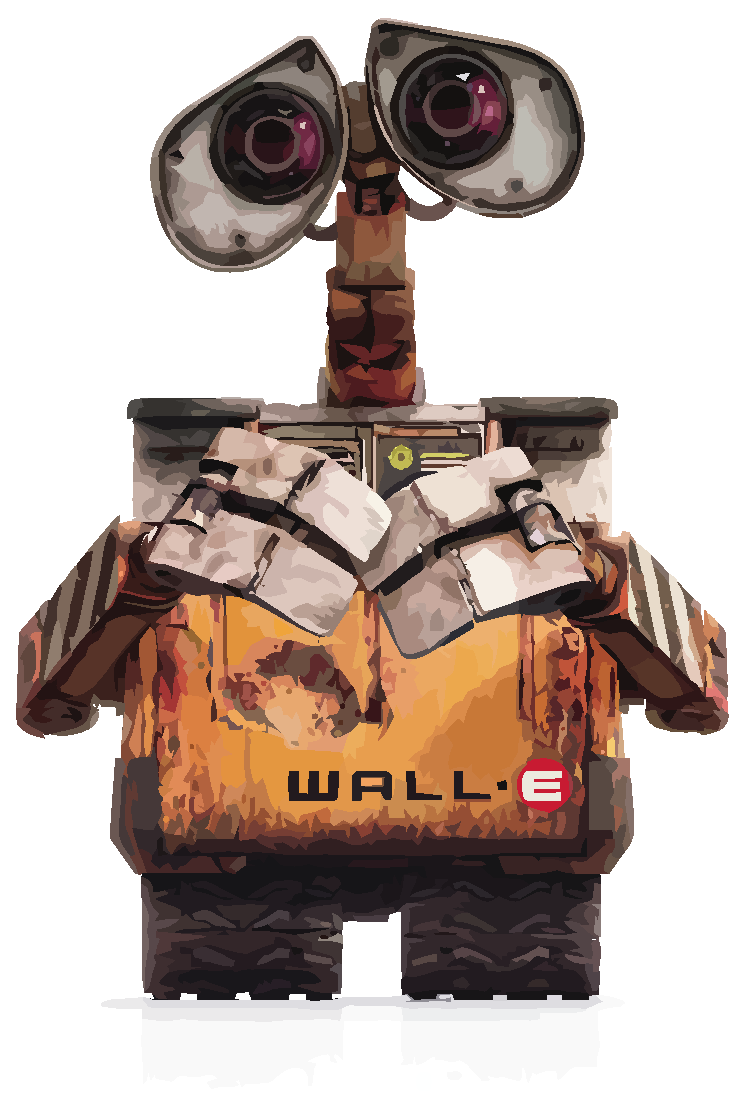
\includegraphics[width=\textwidth]{WallE}
%     \caption{Wall-E}
%     \label{fig:WallE}
%   \end{subfigure}             
%   \begin{subfigure}[b]{0.3\textwidth}
%     
\includegraphics[width=\textwidth]{minion}
%     \caption{Minions}
%     \label{fig:Minnion}
%   \end{subfigure}
%   \caption{Best Animations}
%   \label{fig:animations}
% \end{figure}


% \end{landscape}

\section{General Notations}
\label{sec:defGeneral}
We use the following notations throughout the thesis:
\begin{description}
\item[Vectors, Matrices] We denote column vectors by standard vector notation
  (e.g., \(\vec{x}, \vec{y}\)) and matrices by bold upper-case letters (e.g.,
  \(\mathbf{A}, \mathbf{B}\)). We write \(\vec{b}^{T}\) to convert a vector
  \(\vec{b}\) to a row vector. The length of a vector
  \(\vec{b} = [b_{0}, b_{1}, \dots, b_{n-1}]\) (\textit{norms}) is denoted by
  \(\norm{\vec{b}} = \sqrt{b_{0}^{2} + b_{1}^{2} + \dots + b_{n-1}^{2}}\) for
  Euclidean norm and \(\norminf{\vec{b}} = max(|b_{i}|)\) for infinity norm. The
  \(i\) component of a vector is denoted interchangebly as \(b_{i}\) or
  \(b[i]\).
\item[Groups and Rings] Sets of numbers are denoted as standard (e.g.,
  \(\mathbb{R}\) for set of rational numbers, \(\mathbb{Z}\) for integers), we
  denote \(\mathbb{Z}_{q}\) to be the set of integers modulo \(q\) (in the range
  \((-q/2,q/2]\)).\(\mathbb{Z}[n]\) denotes polynomials of order \(n\) with
  elements in \(\mathbb{Z}\), \(R_{q}\) denotes the ring of polynomial modulo
  \(x^{n} + 1\): \(R_{q} = \frac{\mathbb{Z}_{q}[x]}{x^{n} + 1}\). We use bold
  lower-case to denote an element of the ring \(R_{q}\) (e.g.,
  \(\mathbf{a} \in R_q\)).
\item[Others] We use notation \(x \randomsample D\) when \(x\) is sampled
  uniformly random from the distribution \(D\). If \(x\) is the output of an
  algorithm \(D\), we write \(x \gets D\). Algorithms are \(efficient\) if they
  run in probabilistic polynomial time (PPT). A function is said \(negligible\)
  in \(n\) if it vanishes faster than the inverse of any polynomial.
\end{description}

\section{Lattices}
\label{sec:defLattices}

\subsection{The motivations}
\label{ssub:The motivations}
We choose lattice-based cryptography as the main techniques used in the
thesis for several reasons:
\begin{description}
\item[Provable Security.] Lattice-based cryptosystems' security can be related
  to known computationally hard problems such as Shortest Vector Problem (SVP)
  or Closest Vector Problem (CVP) and therefore we can demonstrate the security
  property in terms of mathematical proofs. For classical system such as RSA,
  there is no proof showing that breaking RSA is as hard as factoring an integer
  even though in many cases the best attack we know is to do such operation.
\item[Quantum Resistance.] In 1994, Shor \cite{shor1994algorithms} showed that
  we can write a program with quantum computers to factor a large integer
  into prime factors.The latest D-Wave systems initial deployments show that the
  idea is feasible in near future. If this happens, it has significant
  implications to the currently used public key cryptosystems such as RSA: they
  will be broken. Lattice based cryptography is currently one of the best
  candidates that resists even quantum attacks.
\item[Homomorphic Operations.] Finally, lattice-based cryptography allows us to
  do operations that we could not do before: computing on encrypted data. This
  special type of operatation can provide privacy features in online
  communications.
\item[Research Activities.] Lattice-based systems have been researched actively
  in the last decade and the development has come to the stage that it can be
  implemented and can be used in the foreseable future.
\item[Performance.] Lattice-based cryptography has the potential to give us very
  fast operations and it is a good option for high performance required
  cryptographic application
\end{description}
We will recall some of the mathematics behind lattices (they are actually
mathematical objects). We will look at the definitions and some of the hard
problems that we will base the security on and how to use lattice to build
cryptographic schemes.


% In terms of efficiency, a brief summary is as follows
% \begin{itemize}
%     \item RSA - key length $\tilde{O}(n^3)$, computation $\tilde{O}(n^6)$.
%     \item ECC - key length $\tilde{O}(n)$, computation $\tilde{O}(n^2)$.

% \end{itemize} The comparison was done on some public key cryptosystems, for RSA,
% for example if we want security level of $2^n$.That means any attack on the
% system will need to run in the order of $2^n$ steps.  Then we can try to measure
% what size of key do we need, and how much computation we need to encrypt. For
% RSA, it’s 6th degree polynomial for computation, that increases quickly with n.
% Even for ECC, the key length is the best we can hope for O(n), the computation
% is still quadratic.  The good thing about lattice based cryptography is we can
% reduce both of the key length and the computation at least in the theoritical
% sense, in the asymptotic sense, when n grows to large values, both key length
% and computation grow linear with $O(n)$. In practice, it’s not as good as
% expected.  But it still quite good, for example if we need n ~ 100 bits of
% security, then in terms of computation, we can have cryptosystem that are 100
% times faster than RSA, and  the key length is a bit bigger than RSA. In
% practice, the advantage of lattice based cryptography is the speed of the
% computation rather than the length of the key.

% Regarding provable security, we can say lattice based cryptography starts from
% 1978 when all of the public key started. The Knapsack cryptosystem is worth
% mentioned here as researchers did spend a lot of effort on improving and
% breaking it, however whenever there was an improvement, then came another attack
% and the cryptosystem was never adopted. It’s not until 1996 when Ajai introduced
% the SIS problem, it’s kind of a variant of knapsack, but it came with
% mathematical proof saying that if there is any algorithm that can solve SIS,
% then we can use it to solve hard lattice problems, even worst-case instances!
% This proof make sure there is no easy way to break the cryptographic tools based
% on SIS, specifically Ajtai introduced the hash function based on SIS. It took
% another 10 years until Regev introduced the LWE problem and a cryptosystem based
% on it. And in the last 10 years, we can see that this area has been actively
% researched both in the analysis and the design of different schemes.

\subsection{Lattice Preliminaries}
\label{ssub:The mathematics}
This is an area of mathematics that combines both matrices, vector algebra
and integer variables. The definitions include:

\begin{definition}[Lattice]
  An n-dimensional (full-rank) \emph{lattice} $L(B)$ is the set of all integer
  linear combinations of some \emph{basis} set of linearly independent vectors
  $\vec{b_1},\dots,\vec{b_n} \in \mR^n$:
  \[
    L(B) = \left\{ c_1 \vec{b_1} + c_2 \vec{b_2} + \dots + c_n \vec{b_n} : c_i
      \in \mZ, i = 1, \dots, n \right\}
  \]
  The $ n \times n$ matrix $B = (\vec{b_1},\dots, \vec{b_n})$ is called a basis
  for $L(B)$. There are infinitely many different bases for a lattice.
\end{definition}

\textbf{Example.} Consider a 2-dimensional lattice generated by the basis
$(\vec{b1}, \vec{b2}) = \left( \begin{bmatrix} 1 \\ 2
  \end{bmatrix} \begin{bmatrix} 0 \\ 3
  \end{bmatrix}\right)$
\begin{figure}[h]
  \centering 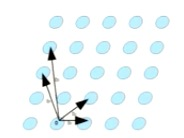
\includegraphics{lattices}
  \caption{Example of a 2-dimensional lattice}
  \label{fig:2dimLattice}
\end{figure}
To generate a lattice from a basis, we compute all the integer multiples of
each vector of the basis, then we add them together to generate new vectors. The
result is an infinite grid of vectors, this grid is a lattice. We can illustrate
two or three dimensional lattice easily, for higher dimensions, it is not
possible to draw the lattice, but the intuition stays the same and all the
algebraic operations can be done easily on the coordinates of the vectors. In
lattice-based cryptography, we work with high dimension lattices ($n > 100$) for
security properties. In fact, we can also say that a lattice is an infinite
group (a group is a mathematical structure, a set with one operation on it.)
with the main operation is addition.

\begin{definition}[Fundamental Paralellepiped]
  For an n-dimensional lattice basis
  $B = \left( \vec{b_1}, \dots, \vec{b_n} \right) \in \mR^{n \times n}$, the
  \emph{fundamental paralellepiped} (FP), denoted $P(B)$, is the set of all real
  valued $[0,1)$-linear combinations of some basis set of linearly independent
  vectors $\vec{b_1}, \dots ,\vec{b_n} \in \mR^n$.
  \begin{figure}[h]
    \centering 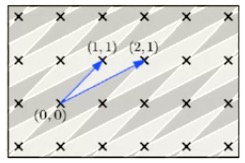
\includegraphics[scale=0.7]{parallelopiped}
    \caption{A paralellogram of 2-dimentional lattice}
    \label{fig:paralellopiped}
  \end{figure}
\end{definition}
In order to determine if a set of vectors is a basis of a lattice, there are
geometric and algebraic approaches.
\begin{lemma}
  There is exactly one \emph{L} point contained in P(B') (the $\vec{0}$ vector)
  if and only if B' is a basis of L.
  \label{lem:parallelopiped}
\end{lemma}
\begin{lemma}
  B' is a basis of L(B) if and only if B'=B.U, for some $n \times n$ integer
  matrix U with $det(U) = \pm 1$, such U is called unimodular matrix.
  \label{lem:detBasis}
\end{lemma}
Where $det(U)$ denotes the determinant of the matrix $U$.  Geometrically, the
determinant computes the area (or volume) of the paralellogram of a lattice. We
can associate each point of a lattice with a paralellogram, consequently, for a
large n-dimensional ball $S$, the number of lattice points in $S$ is
$\approx vol(S) / det(L)$.
\begin{definition}[Determinant]
  \label{def:determinant}
  For an n-dimensional latice $L(B)$, the determinant of $L(B)$, denoted
  $det(L(B))$ is the n-dimensional volume of the FP P(B).
\end{definition}
\begin{lemma}
  For an n-dimensional lattice $L(B)$, we have $det(L(B)) = |det(B)|$.
  \label{lem:determinant2}
\end{lemma}
In cryptography, we are interested in computationally hard problems, there are
some problems related to geometry of lattices that are hard, including Shortest
Vector Problem (SVP) and Closest Vector Problem (CVP).
\begin{definition}
  For an n-dimensional lattice $L$, its \emph{minimum} $\lambda(L)$ is the
  length of the shortest non-zero vector of $L$:
  \[
    \lambda(L) = min(\norm{\vec{b}}: \vec{b} \in L \ 0
  \]
  \label{def:minLattice}
\end{definition}
\begin{theorem}
  [Minkowski's First Theorem] For any n-dimensional lattice $L$, we have
  $\lambda(L) \leq \sqrt(n).det(L)^{1/n}$.
  \label{the:minkowski1}
\end{theorem}
As mentioned, the problem of finding SVP of a lattice is hard as the dimension
grows, in theoretical computer science, this problem is categorized as
NP-hard. In cryptography, we do not use SVP as it is, we use a variant of the
problem, the definition of approximate SVP problem $\gamma-SVP$ follows.
\begin{definition}
  [$\gamma$-SVP problem] Given a basis $B$ for an n-dimensional lattice $L$,
  find $\vec{b} \in L$ with $0 \leq \norm{\vec{b}} \leq \lambda(L)$.
  \label{def:gammaSVP}
\end{definition}
As $\gamma$ increases, the problem becomes easier. We have good algorithms to
find $\gamma$-SVP as follows
\begin{itemize}
\item For $\gamma \geq 2^{O(n)}$: LLL algorithm solves in Poly(n) time.
\item For $\gamma \leq O(1)$: NP-hard, it is not likely that there exists
  Poly(n) algorithm to solve the problem.
\end{itemize}
In cryptography, many systems depend on this $\gamma$-SVP problem, where
$\gamma$ is in between the two extremes $\gamma \approx O(n^c)$. Even with this
factor, the best algorithm (including quantum ones) still take $2^{O(n)}$ time
to solve $\gamma$-SVP. ( In classical cryptosystems for example RSA, the best
algorithm to solve the integer factorization problem take
$\approx O(2^{n^{1/2}})$ in time, this is why we need 4096 bits key to obtain
about 64 bits of security for lattices).

\subsection{q-ary lattices and SIS problem}
\label{sub:q-ary lattices and SIS problem}
There are many useful subclasses of special lattices, in cryptography, we often
use one of them called \emph{q-ary} lattices, which relate to a problem called
Short Integer Solution - SIS (This is a hard problem used in many cryptographic
design, our ZKP technique is also based on a variant of this problem). Recall
that our motivation for lattice-based cryptosystem is the hardness of
$\gamma-SVP$ problem given a basis $B$. It is critical to initially chose the
basis $B$ to make sure that solutions to such hard problem is hard to find. (As
there are easy instances of $\gamma-SVP$, even for $\gamma=1$. We need a way to
generate \emph{random} lattices' bases for which $\gamma-SVP$ is hard to solve
'on-average'. One possible answer is from \cite{ajtai1996generating}: a random
\emph{q-ary} lattice, based on this, we can prove how hard it is to find short
vectors in it.

\begin{definition}[Ajtai's perp lattices]
  Given an integer \emph{q} and a uniformly random matrix
  $A \in \mathbb{Z}_{q}^{n \times m}$, the \emph{q-ary} perp lattice
  $L_q^\bot(A)$ is defined by:
  \[
    L_q^\bot(A) = \left\{ \vec{v} \in \mathbb{Z}^m : A.\vec{v} = \vec{0} \mod \
      q \right\}
  \]
\end{definition}
It might not be clear from the definition of lattices, but the set of all vector
$\vec{v}$ actually forms a lattice. They can be generated by some basis, and
there is a fast algorithm to compute such basis. The parameters for these
lattices are $A$ and $q$, we can choose a lattice to work on by selecting random
values for the parameters. This particular set of \emph{q-ary} lattices is nice
because Ajtai mathematically proved that: If there is an algorithm to break the
$\gamma-SVP$ problem for these lattice, then we could use the algorithm to break
$\gamma-SVP$ for any lattices. This is the \emph{worst-case to average-case}
security reduction and gives us confidence that the problem is hard on average.
\begin{definition}[Small Integer Solution (SIS) problem]
  $SIS_{q,m,n,\gamma}$ Given n and matrix $A$ sampled uniformly in
  $\mathbb{Z_q^{n \times m}}$, find $\vec{z} \in \mathbb{Z}^{m \times n}$ such
  that $A\vec{v} = \vec{0}$ and $\norminf{v} \leq \beta$.
  \label{def:SISProblem}
\end{definition}
Informally, SIS is just the name given to the $\gamma-SVP$ problem for the
particular \emph{q-ary} lattices. $\beta$ is the approximation parameter, it
tells us how short the lattice vector should be. Some relations between SIS and
$\gamma-SVP$
\begin{itemize}
\item $det(L_q^\bot(A)) = q^n$
\item By Minkowski's Theorem, $\lambda(L_q^\bot(A)) \leq \sqrt{m}$, for
  $m \geq n \log q$. So to solve SIS, we need to find vectors not much longer
  than $\sqrt{m}$.
\item We can relate $\gamma$ of SVP to $\beta$ of SIS:
  $\gamma \approx \beta/\sqrt{m}q^{n/m}$.
\end{itemize}

\subsection{A cryptographic example}
\label{sec:ajtaiHash}
Cryptographic hash functions have many applications in many security contexts to
provide authenticity and integrity. One of the main properties of cryptographic
hash functions is collision resistant: it is hard to find 2 message inputs that
produce same hash value output. The current constructions being used in practice
are not lattice-based but base on non-linear boolean functions. We discuss how
to construct one variant from lattice and demonstrate the relevant techniques
that will be used during in the security proofs and parameter choices of the
thesis. The security of this function is directly related to the hardness of
the SIS problem that we saw before
\begin{definition}[Ajtai's Hash Function.]
  Pick $A=(\mathbf{a_{i,j}}) \randomsample \mathbb{Z}_q$ ($A$ is the function
  'public key'). Given $\vec{x} \in \mathbb{Z}^{mn}$ having 'small' coordinates
  ($\norminf{\vec{x}} \leq d$), the hash function out put is defined as
  \[
    g_{q,m,n,d,A}(\vec{x}) = A . \vec{x} \mod \ q
  \]
  \label{def:Ajtai's Hash Function}
\end{definition}
We see that from a long input vector, we obtain a short output vector, that is
our hash value. We can choose the parameters to make sure that constraint is
satisfied. The important question is how do we determine the security of this
function, or how can we know that this function is collision resistant. We
introduce this concept of security reduction, which is used frequently in
lattice-based cryptography's security proofs. We show that if there
was an algorithm to find a collision in this hash function, then we could use
such an algorithm to solve a hard lattice problem. In our case, we know that SIS
was analyzed by Ajtai and shown to be hard based on good foundations. What we
are going to show here is, if we can find a collision efficiently in this hash
function, we could also efficiently find a way to break the SIS problem, that
would contradict the hardness of SIS. Based on this contradiction we can
conclude that there must not exist any efficient algorithm to find collision for
the hash function.
\begin{theorem}
  Collision-Resistance of $g$ is at least as hard as $SIS_{q,m,n,\beta}$ with
  $\beta = 2d$.
  \label{the:ajtai hash}
\end{theorem}
\begin{proof}
  Suppose there was an efficient collision-finder attack algorithm $CF$ for
  function $g$: Given a random instance $(A,q)$, $CF$ outputs
  $\vec{x_1} \neq \vec{x_2}$ such that $A\vec{x_1} = A\vec{x_2}$.

  We then can use $CF$ to build another algorithm $S$ that solves SIS problem
  for any instance $(A,q)$:
  \begin{itemize}
  \item Runs $CF$ on $(A,q)$ to get $\vec{x_1},\vec{x_2}$.
  \item $S$ outputs solution for SIS problem: $\vec{v} = \vec{x_1} - \vec{x_2}$.
  \end{itemize}

  The algorithm works because $A\vec{v} = A\vec{x_1} - A\vec{x_2} = \vec{0}$,
  i.e., $\vec{v}$ is in the lattice $L_q^\bot(A)$ and
  $\norminf{\vec{v}} \leq \beta$, where $\beta = 2d$ (When we add/substract
  vectors ,the result vector's length is upper bounded by the sum of the lengths
  of the vectors). Moreover, $S$ is efficient as $CF$ is efficient (run-time
  $T_S \approx T_{CF})$.
\end{proof}
This is the first application of lattices in cryptography and it actually
started the other modern techniques. The next important questions are
\begin{itemize}
\item How should we choose the parameters to get a given security level.
\item How secure is SIS problem related to $\gamma-SVP$ problem.
\end{itemize}

\subsection{Security of lattice-based cryptography}
\label{sec:latticeSecurity}
Lenstra–Lenstra–Lovász (LLL) and various improvements are the main ways to
access the security of lattice-based systems (by access the security of
underlying problems such as SVP .or $\gamma-SVP$). From there, it allows us to
choose the size of the parameters for the problem (such as dimensions) in order
to give guarantee of security against the best known attack.

We first recall this important concept related to lattices that is used in LLL:
Gram-Schmidt Orthogonization (GSO)
\begin{definition}
  [GSO] For a lattice basis
  $B = \left( \vec{b_1}, \vec{b_2}, \dots, \vec{b_n} \right)$, its GSO is the
  matrix of vectors
  $B^* = \left( \vec{b}_1^*, \vec{b}_2^*, \dots, \vec{b_n^*} \right)$ defined by
  $\vec{b_1^*} = \vec{b_1}$ and for $i \geq 2$,
  $\vec{b_i^*} = \vec{b_i} - \sum_{j=1}^{i-1}{\mu_{i,j}.\vec{b_j^*}}$, where
  $\mu_{i,j} = \frac{\langle \vec{b_i}, \vec{b_j^*} \rangle}{\langle
    \vec{b_j^*},\vec{b_j^*} \rangle}$.
  \label{def:GSO}
\end{definition}
GSO is basically a way to convert a basis that we have (that are not orthogonal)
into another set of vectors are orthogonal. Figure \ref{fig:gso} shows an
example of GSO in 2-dimension
\begin{figure}[h]
  \centering 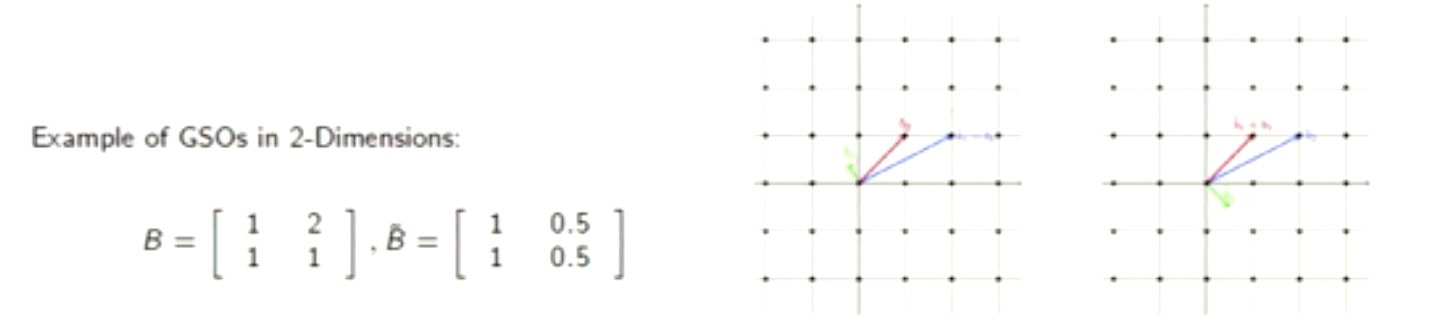
\includegraphics[scale=0.3]{gso}
  \caption{Example of GSO in 2-dimensions}
  \label{fig:gso}
\end{figure}
GSO is used as part of the LLL algorithm to find short vector of a lattice.
Note that the $GSO(B)$ is not another basis for the original lattice, it is just
a related matrix, it has the same determinant as the original one.

% Once we have done the transformation from $B$ to $B^* = GSO(B)$, we can also
% write the relation between the two of them algebraically as in Figure \ref{}
% \begin{figure}[h]
%   \centering 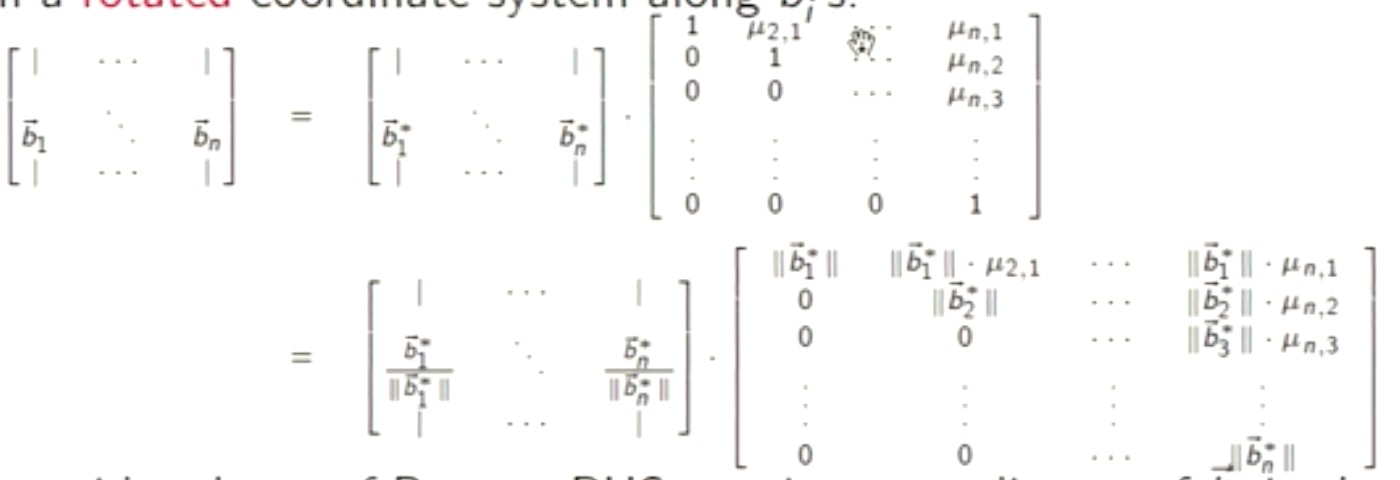
\includegraphics[scale=0.3]{gsoMatrix}
%   \caption{GSO algebraic relation}
%   \label{fig:GSOAlgebra}
% \end{figure}
% We can intepret the second relation as a rotated coordinates system. Another
% nice observation we can have from this matrix representation is the 0s in the
% matrix implies the determinant of the lattice:
% \[
%   det \ L(B) = |det(B)| = |det(B^*)| = \prod_{i=1}^{n}\norm{\vec{b_i^*}}
% \]

% Back to our LLL discussion, this is the main algorithm to find short vectors in
% lattices, and therefore the main type of attack against lattice-based
% cryptosystems in practice, the other approach is exhaustive search. The best
% algorithm is the combination of the 2 approaches to trade off the runtime verse
% the approximation factor. We will discuss this algorithm (BKZ) in a later
% section.

\subsubsection{LLL algorithm}
\label{sec:LLLalgorithm}
Lenstra–Lenstra–Lovász (LLL) algorithmnot only finds short vectors but also
manipulate the basis of the lattice into another basis of the lattice. Given
some basis as a input to LLL (whose vectors are long), LLL makes sequential
modifications to the basis, every modification keeps it still a basis of the
lattice and improve it a little bit. When the improvement is repeated, the sizes
of the vectors of the basis are also reduced until it ends with a matrix that
cannot be improved anymore. That is the output of LLL: a basis of the lattice
that is much better than the original input, in the sense that it has much
shorter vectors.

In more details, LLL looks at the property of the GSO of the basis to make the
basis vectors 'approximately' orthogonal. The size of the GSO basis tells us the
length of the projections of one vector along the earlier vectors. The larger
these are, the less orthogonal the basis vectors are because they have bigger
components along the earlier vectors. LLL tries to reduce those coefficient
(projection coefficients), to make them more orthogonal, that will also make
them shorter. There are 2 tests that LLL does to see how orthogonal the basis
vectors are

\begin{description}
\item [LLL property 1.] Take the current basis of the lattice and computes the
  GS coefficients $\mu_{i,j}$. It checks $|\mu_{i,j}| \leq 1/2$, that means the
  length of the projections on the previous vectors are at most half of the
  actual full vector. If this condition is not satisfied, LLL modifies the basis
  until the condition passes.
\item [LLL property 2.] The algorithm looks at the large remaining component
  $\norm{\vec{b_{i+1}^*}}$ of $\vec{b_{i+1}}$ after removing components along
  $\vec{b_j^*}$'s ($j < i + 1$) and check
  \[
    \norm{\vec{b_{i+1}^*}+\mu_{i+1}\vec{b_i^*}}^2 \geq \delta
    . \norm{\vec{b_i^*}}^2
  \]
  for all $i=1,\dots,n-1$ and for some constant
  $\delta$($1/4 \leq \delta \leq 1$).

  Informally, the second check is a bit more complex: LLL looks at the last 2
  components of each vector. If we take a vector $\vec{b_i}$ and decompose it
  into all the projections along the previous $\vec{b_j^*}$ and check the the
  sum of the orthogonal component and the one previous to that: For example, if
  we look at $\vec{b_{i+1}}$, then we check
  $\norm{\vec{b_{i+1}^*}+\mu_{i+1}\vec{b_i^*}}^2$. If this quantity is big
  enough, it is an indication that we have a lot left over after we remove the
  components along the previous one. The bigger this length is, the more
  orthogonal the basis becomes. The algorithm tries to make it big enough.  The
  parameter $\delta$ of the algorithm decides this magnitude (the larger
  $\delta$ is, the better result returned from the algorithm).

  This check is also done for all the vectors of the basis. If it is not
  satisfied, then again LLL does some changes to make sure the test passes.
\end{description}

When the algorithm runs, the 2 checks keep fighting between each
other. Eventually, it hopes to get to a stage where both of the checks satisfy
simultaneously and the algorithm stops and outputs the basis. (Algorithm
\ref{alg:LLL})
\begin{definition}
  A basis $B$ for lattice $L$ is $\delta-LLL$ reduced if both LLL properties 1
  and 2 are satisfied.
  \label{def:LLL}
\end{definition}

\begin{algorithm}
  \caption{LLL algorithm}
  \label{alg:LLL}
  \begin{algorithmic}[1]
    \Procedure{LLL}{$B$} \State Compute GSO $B*$ for B.  \For {$(i=2,\dots,n)$}
    \For {j = i - 1 to 1} \State
    $c_{i,j} \gets \lceil{\frac{\langle \vec{b_i}, \vec{b_j^*} \rangle}{\langle
        \vec{b_j^*},\vec{b_j^*}\rangle}}\rfloor$ \State
    $\vec{b_i} \gets \vec{b_i} - c_{i,j}\vec{b_j}$ \EndFor \EndFor \If
    {$\norm{\vec{b_{i+1}^*}+\mu_{i+1}\vec{b_i^*}}^2 \geq \delta
      . \norm{\vec{b_i^*}}^2$} \State Swap $\vec{b_i}$ and $\vec{b_{i+1}}$.
    \State Go back to step 2.  \Else \State Return B \EndIf \EndProcedure
  \end{algorithmic}
\end{algorithm}
Note that in the algorithm we take the rounded multiple of $\vec{b_j}$, this
important operation helps the algorithm maintaining the vectors to be basis of
the lattice. As the lattice consists of only integer multiples of all the basis
vectors: if we add an integer multiple of $\vec{b_j}$ to $\vec{b_i}$, we still
end up with another lattice vector, we can also show that the new matrix is also
a basis of the lattice. In other words, if we add fraction of $\vec{b_j}$, it is
not lattice point anymore. Also, due to this rounding error, instead of having a
precisely orthogonal vectors in the result matrix, we only obtain an approximate
orthogonal matrix.  For more intuition of the algorithm, we refer reader to
\cite{lenstra1982factoring}. Last but not least, the loop of the algorithm was
shown to always terminate in polynomial time!
\begin{theorem}
  [LLL run time] The number of iterations of LLL on an input basis B before
  termination is at most
  \[
    n^2.\log{(\max{\norm{\vec{b_i}}})} / \log{(1/\sqrt{\delta})}.
  \]
  For any constant $1/4 < \delta < 1$, this is polynomial in bit length of the
  algorithm input. Moreover, the run-time for each iteration is also polynomial
  in the input bit length. Overall, run-time is polynomial in input length, or
  LLL is efficient!
  \label{theo:LLLRunTime}
\end{theorem}

\subsubsection{LLL solution to $\gamma-SVP$}
\label{sec:LLLsolution}
The question is how short are the vectors of LLL's output, or what kind of
approximate SVP can LLL solve: If we run LLL on some basis, we get back a
reduced basis, and we take the shortest vector in that result basis. How long is
that vector compare to the shortest vector in the lattice.
\begin{theorem}
  [Short vector from LLL]. The LLL algorithm solves in polynomial time
  $\gamma-SVP$ for $n-dim$ lattices, with $\gamma < 2^{(n-1)/2}$.
  \label{theo:LLLShortVector}
\end{theorem}

% \begin{proof}
%   The idea is to combine both of the relations in LLL to show that if we take
%   the ratio of the length between to successive Gram-Schmidt vectors of the
%   lattice: $\frac{\norm{\vec{b_{i+1}^*}^2}}{\norm{\vec{b_i^*}^2}}$, it is always
%   going to be at least $(\delta - 1/4)$. It means that when we go from $i$ to
%   $i+1$, the length of $\vec{b_i^*}$ cannot decrease by more than a factor of
%   2. After $n$ steps, the length drops $2^n$ times. One of the property of the
%   Gram-Schmidt basis mentioned was: the last Gram-Schmidt's vector length is a
%   lower bound of the length of the shortest vector in the lattice: $\vec{b_1^*}$
%   is always less than the length of the shortest vector of the lattice. Since
%   $\norm{\vec{b_1^*}}$ can only be at most \todo[inline]{finish proof}
% \end{proof}

In summary, the first vector of LLL output is bounded by
\[
  \norm{\vec{b_1^*}} \leq (1/(\delta-1/4))^{(n-1)/2}.\lambda(L)
\]
% The $\delta$ parameter of the algorithm therefore also contribute to
% the output.
We can see that the approximation factor is exponential in the dimention $n$ of
the lattice. Another way to measure how short of output vector of LLL is Hermite
Factor (HF), which is the ratio of the algorithm's output with the $n^{th}$ root
of the determinant of the lattice. Sometimes it is more convinient to use this
measure because the determinant of the lattice sometimes is easy to compute,
whereas the length of the shortest vector of the lattice is not, in general. In
practice we usually use this as a main measure. Again, LLL gives HF that is
exponential in the dimension $n$. The conclusion is, although LLL runs in
polynomial time, but the approximation factor increases exponentially fast with
the dimension. When the dimension is large, the approximation factor will grow
so fast that LLL is not useful to break the security of underlying
cryptosystems.
\begin{theorem}
  The LLL algorithm solves in polynomial time $\gamma-SVP$ for $n-dim$ lattices,
  with $\gamma \leq 2^{(n-1)/2}$. Can also be shown that Hermite Factor
  $\gamma_{HF} = \frac{\norm{\vec{b_1}}}{det(L)^{1/n}} \leq 2^{(n-1)/4}$
  \label{theo:LLLHF}
\end{theorem}

\subsubsection{LLL in practice}
\label{sec:LLLinPractice}
This section discuss the trade-off between the running time and the length of
the output of the attack. This helps us in selecting parameters for
state-of-the-art lattice attack

In practice we try to improve this bound so LLL can get shorter vector. One way
to do that is to use the fact that, in our analysis, we do worst-case analysis
on the output that LLL can give. In practice, they tend to be shorter than
that. When we run it experimentally (\cite{nguyen2006lll}) on random lattice we
will find that it perform much better than the bound proved. Specifically, $HF$
is close to $1.02^{n-1}$. Although this factor is still exponential in dimension
$n$, this slowth growth allows LLL to be used with large dimension lattices.  In
order to reduce this $HF$ further, we can further modify LLL.  There are several
ways to do that. The basic idea is to combine LLL with exhaustive search
(enumeration algorithm). The best lattice exhaustive search algorithm
(Fincke-Phost/Kannan) does it in time $2^{O(n\log(n)}$, it is even worst than
exponential. There are variants of such method but they all take time at least
exponential with the dimension $n$ (with the expense of using $2^{O(n)}$
memory). In general, all enumeration algorithms are very inefficient. Therefore,
combining LLL with bruteforcing is a more practical approach: BKZ is the typical
algorithm in this category.  BKZ allows trades off between run-time and
approximation factor $\gamma$, LLL is modified by changing the blocksize $k$ of
vectors in the swapping step. As we increase $k$: We search in the lattice of
dimension $k$ using brute force search and then run LLL with smaller dimension
k. We get the 'interpolation' between the two extremes of LLL (corresponding to
$k = 2, \gamma = 2^{O(n)}, T = n^c$) and the enumeration (corresponding to
$k = n, \gamma=1, T = 2^{O(n\log(n)}$)). In between, BKZ can achieve
$\gamma(k) \leq k^{(n-1)/(k-1)}$ with running time
$n^c.k^{O(k)}$. \cite{hanrot2011terminating}. From this trade-off setting, an
attacker then can choose the optimal value of $k$ for particular context: A
lattice-based cryptographic scheme can only be broken if the adversary can find
short enought vectors. This also tells how small $\gamma$ needs to be in order
to defend against such attack:

In summary, given a security level $\lambda$ for a system (i.e., it would take
time $2^\lambda$ for the best attack to work even with the best choice of the
parameter $k$ for BKZ) .  The best approximation factor $\gamma$ that the
algorithm can achieve is related to $\lambda$ as:
\[
  \log(\gamma_{HF}) = \Omega(\frac{n\log^2\lambda}{\lambda})
\]
where $\Omega$ represent asymptotic ``lower than'' condition when the parameters
are large. Overall, we can conclude the \emph{lattice 'rule of thumb'} for
$\gamma-SVP$ using BKZ:
\[
  n = \Omega(\frac{\lambda}{\log^2\lambda}.\log\gamma_{HF}) \approx \lambda
  . \log\gamma_{HF}
\]

\begin{remark}
  The dimension $n$ of a lattice-based cryptosystem needs to be proportional to
  the product of bit-security level $\lambda$ and the $\log$ (base 2) of the
  approximation factor $\gamma_{HF}$.  This factor is a reason behind the long
  keys of such cryptosystems.
  \label{rem:dimension}
\end{remark}

For concrete values of parameters, Chen and Nguyen \cite{chen2011bkz} gave
numerial estimates for Hermite Factor and time for random lattices versus block
size for optimized BKZ variant:

\begin{figure}[h]
  \centering 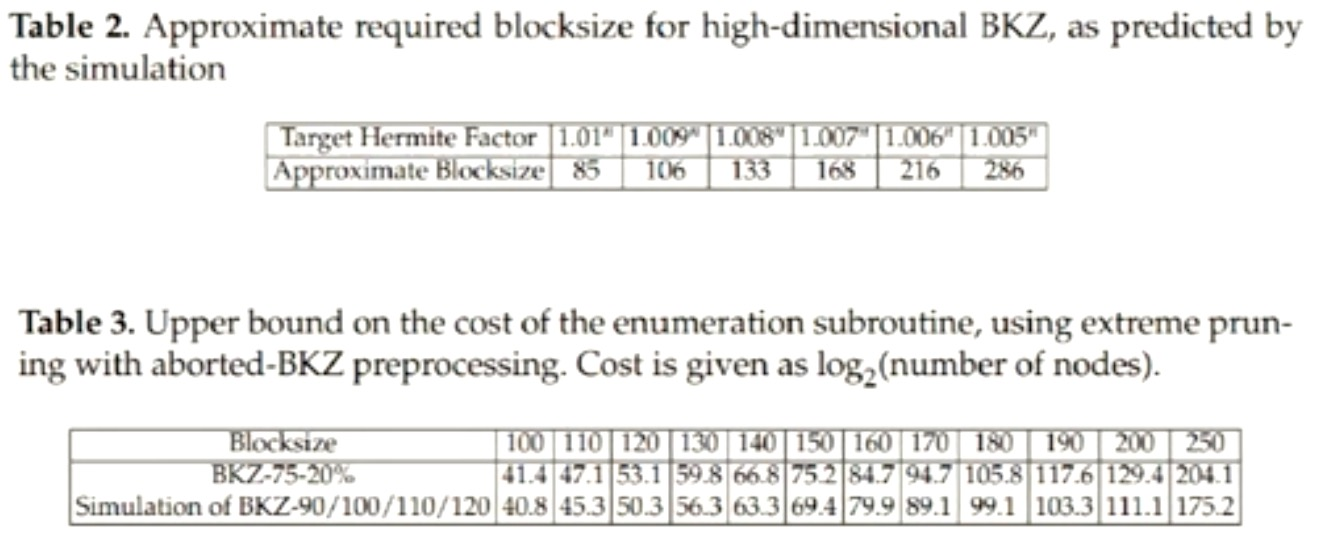
\includegraphics[scale=0.3]{bkzparams}
  \caption{BKZ parameters}
  \label{fig:BKZParams}
\end{figure}

From table 2, for a given $HF$ that we want BKZ to achieve, it gives us the
block size parameter $k$ that need to be used. Note that the $HF$ is much
smaller than what we had for LLL (whose $HF \approx 1.02^{n-1}$ in
practice). Once we have the blocksize, we can look up in table 3 to know the
running time of the algorithm.

\subsection{An example of parameters choice}
\label{sec:parameterChoice}
We discuss Ajtai's hash function as an example of how to choose parameters for
some security level. We showed that if there is an algorithm that can break the
collision-resistance property of the hash function, we can use it to find a
short vector of the SIS problem with length $\beta = 2d\sqrt{m}$. The question
is how do we choose the parameters $q,n,m,d$ for the hash function to get a
given security level $\lambda$ based on the hardness of SIS? According to the
BKZ state-of-the-art attack, to get running time of $2^\lambda$, we can use the
table 3 to derive the blocksize and corresponding Hermite Factor $\gamma_{HF}$.
Then we know the best attacker can compute a non-zero vector $\vec{v}$ in SIS
lattice $L_q(A)$ of norm $\leq l = min(q, \gamma_{HF}.det(L_q(A))^{1/m})$. Then
we can compare $l$ with $\beta$ (or $2d\sqrt{m}$), if $l < \beta$, the attack
will work and otherwise.

There are often ways to optimize such attacks where attacker choose parameters
to minimize the his effort. For example in the attack of SIS problem of
\cite{micciancio2008lattice}, the attacker can look at a subset $m' \leq m$ of
columns of $A$, suppose that he can find a short vector $\vec{v'}$ such that
$A'\vec{v'} = \vec{0} \mod \ q$. He can choose $\vec{v''} = \vec{0}$ and set
$\vec{v} = \vec{v'} + \vec{v''}$. It turns out that there are optimal values
that an attacker can choose for $m'$ that minimize the length $l(m')$ for
$\vec{v'}$.  Specifically, $l(m') = min(q,\gamma'_{HF}.det(L_q(A))^{1/m'})$ is a
function of $m'$, when we graph this function, it is as illustrated in Figure
\ref{fig:bestAttack}.
\begin{figure}[h]
  \centering 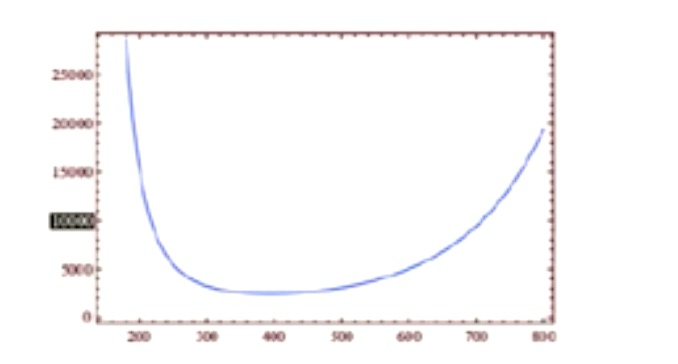
\includegraphics[scale=0.3]{bestattack}
  \caption{Choosing best m' for SIS attack for parameters
    $\delta = 1.01, q=4416857, n=100$}
  \label{fig:bestAttack}
\end{figure}
We can see that at some point $m'$ there is some minimum value for the length of
the vector we can get with BKZ, this is the value that an attacker want to
choose. Denote $m^*$ to be this optimal selection, we have
$l(m^*) = min(q, 2^{2.sqrt{n\log q\log \delta}})$. The condition that the attack
fails is $l(m^*) > \beta$, so
\[
  q \geq \beta = 2d\sqrt{m} \ \text{and}\ n \geq \frac{\log^2(\beta)}{\log q
    \log(\delta)}
\]
We have looked at the best practical algorithms to attack lattice problems (LLL
and its variants). In theory, there is also Ajtai's proof where it said there is
a relationship between how hard it is to solve the SIS problem for random
matrices. The connection between this kind of average case and the worst-case
complexity of lattice problem in general (lattices that are completely unrelated
to the \emph{q-ary} ones) is the theoretical base behind lattice-based
cryptography. We present Ajtai's average-case to worst-case connection Theorem
(1996, improved by \cite{gentry2008trapdoors}).

\begin{theorem}
  [Ajtai's hardness proof for SIS.] If there is an algorithm $A$ that solves
  $SIS_{m,n,q,\beta}$ in poly-time, for some non-negligible fraction of input
  matrices $G \in \mathbb{Z_q^{m \times n}}$, then there is an algorithm $B$
  that solves $\gamma-SVP$ in polynomial time for all input lattices $L$ of
  dimension $n$ with:
  \[
    \gamma = O(\beta\sqrt{n}), q = \omega(\gamma\sqrt{\log n})
  \]
  \label{theo:AjtaiHardness}
\end{theorem}

Although the theorem does not directly gives us concrete information to choose
parameters to secure a cryptosystem like we discussed previously, it does give
us the qualitative confidence in the security of the problem.

\section{Learning With Error}
\label{sub:LWE}
    \begin{description}
        \item[intro.] Last chapter we discuss the complexity of the hard
            problems that are used as the basis of security for lattice-based
            cryptography. In particular we looked at the LLL algorithm that is
            used to find short vectors in lattices. This chapter we discuss
            another use for lattice-based cryptography. So far we have seen how
            to construct hash function, another main tool in cryptography is
            encryption: how to provide confidentiality. We will see that we need
            to use a slightly different type of lattice problem instead of SIS
            problem: we introduce Learning With Error (LWE) problem, which is
            much more suitable than SIS for building the encryptions based on
            it. We will discuss how to use LWE to build symmetric key encryption
            as well as how to modify it to get public key encryption (Regev
            cryptosystem). This cryptosystem is a very important foundation, it
            is the basis for a lot of further
            developments in the area. We first look at the Learning With Error
            (LWE) problem

            In the SIS problem, given a matrix $A$, it is asked to find
            a short vector $\vec{v}$ such that $A\vec{v} = \vec{0}$. The
            cryptographic hash function that is based on SIS
            is constructed such that it can take arbitrary inputs and produces
            collision-resistance outputs. When we do that, we always have a
            many-to-one
            function nature in the construction:
            given an output, it is not possible to derive the original
            input. This many-to-one property is not useful in encryption
            context: we cannot decrypt the ciphertext to the original plaintext
            using such method. In encryption contexts, we usually have the
            reverse situation: the set of possible inputs might be a lot smaller
            than the set of possible outputs. The function serving encryption
            should be at least a one-to-one function that map a plaintext to a unique
            ciphertext. Or we can even have one-to-many functions that map a
            plaintext to many possible ciphertexts, as long as there is no
            intersection between the ciphertext output sets, we are still able
            to decrypt correctly. We see such situation in non-deterministic
            cryptosystems where the encryption function takes the message as
            well as a randomness factor as inputs. Actually, almost all
            encryptions being used in practice are somehow randomized, the main
            reason is to stop the leakage of
            information given many ciphertexts. A deterministic crypto scheme
            can be exploited if the plaintext space is small, for example,
            consider a situation where Alice sends deterministic encrypted
            messages
            to her
            agent Bob
            everyday to instruct him to sell or not to sell some of her
            companies' shares.
            An attacker capturing the ciphertexts of several days can easily
            distinguish such
            decisions without having to decrypt the messages at all. This is one
            of the important property that we want to have in cryptogsystems:
            indistinguishability, also known as IND-CPA. This type of security
            requires that the adversary cannot distinguish the ciphertexts even
            when he know all the posibilities of the plaintexts.

            We introduce LWE problem \cite{regev2005lattices} that allows us to construct
            one-to-one or
            one-to-many functions. The main idea behind LWE is, given a
            secret vector and a random lattice point with some 'small noises' added to
            the point, it is infeasible for an attacker to learn anything from
            the output but it is easy for the data owner with the secret to
            revert back the original point. The description of LWE follows.
        \item [LWE] Fix integers $q, m, n$ and initialize the matrix
            $A^{m \times n}$. Note that the matrix
            $A$ is a bit different from SIS regarding its dimension,
            this is just for convenient representation purpose.
            $q$ is still the
            modulus of $a_{i,j}$, where $a_{i,j} \randomsample
            \mathbb{Z}_q$. Let $\vec{s}^T = \left[ s_1,s_2,\dots,s_n
            \right]$ be a vector of independent uniformly random
            elements of $\mathbb{Z}_q$, this is the secret element that
            corresponds to the secret key of the cryptosystem. Let
            $\vec{e}^T = [e_1,\dots,e_n,\dots,e_m]$ be a vector of
            independent 'small' integers, each sampled from a
            probability distribution $\chi_{\alpha q}$. By 'small', we
            mean $\norminf{e_i} \leq \alpha . q$ for some parameter
            $0 < \alpha < 1$. Typically, $\chi_{\alpha q}$ is chosen from a
            Normal (Gaussian) distribution with standard deviation
            $\approx \alpha . q$. (From the implementation point of view,
            one way to do such sampling efficiently is to take
            the real samples from a normal continuous distribution and round it
            to the neareast integers, the mean is set to 0 to make sure the
            samples are small).

            Let
            \[
                \vec{y} = \begin{bmatrix}
                    a_{1,1}, a_{1,2},\dots, a_{1,n}\\
                    a_{2,1}, a_{2,2},\dots, a_{2,n}\\
                    \dots,\dots, \dots,\dots\\

                \end{bmatrix}
            \]
            \todo[inline]{finish this}

            We discuss two
            variants of the LWE problems to be used in cryptosystems: Search-LWE
            and Decision-LWE problems.

            \begin{definition}
                [Search-LWE Problem.] Given $q,m,n,\alpha$ and a matrix
                $A \randomsample \mathbb{Z}_q^{m \times n}$ and $\vec{y} =
                A.\vec{s} + \vec{e} \mod q$ (with $\vec{e} \randomsample
                    \chi_{\alpha q}^m$ and $\vec{s} \randomsample
                \mathbb{Z}_q^n$), find $\vec{s}$.
                \label{def:Search-LWEProb}
            \end{definition}

            \begin{definition}
                [Decision-LWE Problem.] Given $q, m, n,
                \alpha$ and $A \randomsample \mathbb{Z}_q^{m \times n}$,
                $\vec{y}$, distinguish between the following two scenarios
                \begin{itemize}
                    \item \emph{Real Scenario:} $\vec{y} = A.\vec{s} +
                    \vec{e} \mod \ q$ (with $\vec{e} \randomsample
                    \chi_{\alpha q}^m$  and $\vec{s} \randomsample
                    \mathbb{Z}_q^n$)
                \item \emph{Random Scenario:} $\vec{y} \randomsample
                    \mathbb{Z}_q^m$.
                \end{itemize}
                \label{def:Decision-LWEProb}
            \end{definition}

            From an attacker's point of view, DLWE is simpler than
            SLWE. In other words, cryptosystems that rely on DLWE give stronger
            security assurance because if the attacker cannot solve the simpler
            problem, he is not able to solve the hard one. Also, we will see
            that with DLWE, we can construct more efficient cryptosystems. In
            regards to the hardness of the two problems,
            we easily see that the SLWE is hard if any poly-time attacker can
            find $\vec{s}$ with a negligible probability. For DLWE, we can
            say that it is hard if the adversary cannot solve it better than
            by merely guessing. One way to quantify how good is an attacker's
            alogirithm $D$ is to look at the \emph{distinguishing advantage}
            $Adv(D)$:
            \[
                Adv(D) = Pr_{\vec{y}\randomsample Real}[D(A,\vec{y}) = Real] -
                Pr_{\vec{y}\randomsample Random}[D(A,\vec{y}) = Real]
            \]
            From such definition, we say that DLWE is a hard decisional problem
            if there exists no
            algorithm $D$ that runs in time $T(D) \leq 2^\lambda$ and has
            $Adv(D) \geq 2^{-\lambda}$ for a large $\lambda$. We will discuss
            the correspondence of DLWE with
            breaking the encryption scheme in terms of the
            indistinguishability that we mentioned.

        \item [Security of LWE Problem.] An average-case to worst-case
            connection similar to Theorem (\ref{theo:AjtaiHardness}) for SIS
            problem can also be established for LWE (\cite{regev2005lattices})
            \begin{theorem}
                If there is an algorithm $A$ that solves $DLWE_{q,m,n,\alpha}$
                in poly-time, with non-negligible distinguishing advantage, for
                $\alpha . q > 2 \sqrt{n}$. Then there is a quantum algorithm
                $B$ that solves $\gamma-GapSVP$ in polynomial time for all input
                lattices $L$ of dimension n with:
                \[
                    \gamma = O(n/\alpha)
                \]

                \label{theo:RegevLWEHardness}
            \end{theorem}
            Theoretically we have strong reason to believe that LWE
            is hard. The theorem even says that it links the security of LWE to
            the quantum security of the shortest vector problem. It therefore
            gives us more confidence to use LWE as the basis for quantum
            resistant cryptographic technique. In practice, the best known
            attack against LWE is to reduce the problem to the SIS problem:
            Given a LWE instance $(A \in \mathbb{Z}_q^{m \times
            n},\vec{y} \in \mathbb{Z}_q^m)$:
            \begin{itemize}
                \item Find a short non-zero vector $\vec{v}$ in the SIS lattice
                    $L_q^\bot(A^T)$ with $\norm{v} \leq \beta$. That is,
                    $A^T.\vec{v} = \vec{0} \mod q$.
                \item Compute $e' = \vec{v}^T.\vec{y} \mod q$ and check:
                    \begin{itemize}
                        \item In 'Real DLWE Scenario', $e'$ is small
                        \item In 'Random Scenario', $e'$ is not small
                    \end{itemize}
            \end{itemize}

            In other words, solving $DLWE_{q,m,n,\alpha}$ reduces to solving
            $SIS_{q,m,n,\beta=1/\alpha}$, therefore to secure the system based
            on DLWE, we must choose parameters so that $SIS_{q,m,n,\beta}$ is
            hard. (The smaller the noise we choose for DLWE, the larger the
            $\beta$ becomes, or $\gamma-SVP$ is easier, which is expected).
            Also, the condition of $\alpha q > 2\sqrt{n}$ is also important as
            when the noise become small enough, it turns out that there are
            efficient algebraic attacks against LWE.



        \item [Symmetric-Key Encryption from LWE.] We present a randomized cryptosystem
            based on LWE
            \begin{description}
                \item[Key Generation - KeyGen.] Fix integers $q, n$. Pick a secret key
                    $\vec{s} \randomsample \mathbb{Z}_q^n$.
                \item [Encryption - Enc.] Fix integers $t,l$. Given a message
                    $\vec{m} \in \mathbb{Z}_t^l$:
                    \begin{itemize}
                        \item Pick $A \randomsample \mathbb{Z}_q^{l \times n}$
                            and 'small' noise $\vec{e} \randomsample
                            \chi_{\alpha q}^l$.
                        \item Compute $\vec{c} = A.\vec{s} + \vec{e} + \lceil
                            q/t \rfloor . \vec{m} \mod \ q$.
                        \item Return ciphertext $(A, \vec{c}$.
                    \end{itemize}
                \item [Decryption - Dec.] Given a ciphertext $(A,\vec{c})$ and a
                    secret key $\vec{s}$:
                    \begin{itemize}
                        \item Compute $\vec{c'} = \vec{c} - A.\vec{s} \mod \ q$.
                        \item Compute $\vec{c''}$ by rounding coordinates of
                            $\vec{c'}$ to the neareast multiple of $\lceil q/t
                            \rfloor \mod \ q$. This step exploits the fact that
                            $\vec{e}$ is a 'small' vector rather than a random
                            one.
                        \item Return plaintext $\vec{m} =
                            \frac{\vec{c''}}{\lceil q/t \rfloor}$
                    \end{itemize}

                \item [Correctness.] Decryption is correct if the rounding step
                    succeeds, or if all the noise coordinates $e_i$ of
                    $\vec{e}$ is sufficiently small:
                    \[
                        e_i < \frac{1}{2} . \lceil q/t \rfloor \approx
                        \frac{q}{2t}
                    \]
                    If the noise distribution $\chi_{\alpha q}$ is a normal
                    distribution with standard deviation $\alpha q$, the
                    probability that the noise exceeds $\frac{1}{2t\alpha}$ in
                    magnitude is $p_e \approx 2.\left( 1 - \Phi\left(
                            \frac{1}{2t\alpha}
                    \right) \right)$, where $\Phi$ is the cumulative
                    distribution function of the standard normal distribution
                    (mean 0 and standard deviation 1). Therefore, to assure
                    correctness, we need this probability to be sufficiently
                    small, the following \emph{correctness condition} must
                    holds:
                    \[
                        t << \frac{1}{2\alpha}
                    \]
                    We can see that the larger the noise is, the smaller our
                    message space becomes. However, when the noise is large, LWE
                    is harder as well: security goes up when noise increase.
                    Generally, in lattice-based cryptosystems, there is this
                    trade-off between security and the size of messages to
                    encrypt.

                \item [Security.] This section discusses how to analyze the
                    security of lattice-based cryptosystems. Our goal is to show
                    that if an adversary can break the encryption scheme's
                    security, then he can also break DLWE problem, which will be
                    the hard problem that relate to lattice problems that we
                    known that are hard (SIS or $\gamma-SVP$). The standard
                    security model that is used in our analysis would be
                    indistinguishability security against Chosen Plaintext
                    Attack (IND-CPA). The formal 'security game' is defined between a
                    challenger $Ch$ and the attacker $B$ against the encryption
                    scheme

                    \begin{description}
                        \item[CPA Security Game.] The game is defined as
                            follows.
                    \begin{itemize}
                        \item The challenger $Ch$ runs $Keygen$ algorithm and
                            obtains a
                            secret key $\vec{s}$.
                        \item The attacker $B$ is given access to an 'encryption
                            oracle': $B$ can submit a plaintext $\vec{m}$
                            and get back from $Ch$ a ciphertext $(A,C) =
                            Enc(\vec{}, \vec{m})$. $B$ can query the oracle as
                            many times as he wants. When B finishes the query
                            phrase, he submits a pair of 'challenge messages'
                            $\vec{m_0^*},\vec{m_1^*}$.
                        \item Challenger picks a random bit $b \randomsample
                            U(0,1)$, computes a 'challenge ciphertext'
                            $(A^*, C^*) = Enc(\vec{s}, \vec{m_b^*})$ for the
                            challenge message selected by $b$, and sends
                            $(A^*, C^*)$ to  $B$.
                        \item $B$ can continue querying the 'encryption oracle'
                            if he would like. Finally, he outputs a guess
                            $b'$ for the bit $b$ chosen by the challenger. The
                            attacker wins the game if $b' = b$.
                    \end{itemize}
                    \begin{definition}
                        [IND-CPA security.] A cryptosystem is IND-CPA secure
                        with a security level $\lambda$
                        if any attack algorithm $B$ with
                        run-time $T(B) \leq 2^\lambda$ can only win the security game
                        with probability $\leq \frac{1}{2} +
                        \frac{1}{2^\lambda}$.
                    (Note that we have to restrict the run-time of the attacker
                    as we know that for any cryptosystem, an attacker with
                    unlimited time can always win the game with probability 1
                    using brute force search.)
                        \label{def:IND-CPA Security}
                    \end{definition}

                \item [Security Reduction from IND-CPA to DLWE.] Given the formal security game,
                    we need to prove that the cryptosystem defined satisfies
                    such model. By applying the security reduction technique, we demonstrate
                    that if an attacker could somehow break the cryptosystem,
                    then he could also solve DLWE, which was proved (Regev,
                    2005) to be a
                    lattice-related hard problem:

                Suppose there was
                    an efficient IND-CPA attack algorithm $B$, breaking
                    $2^\lambda$ security of the LWE encryption scheme:
                    \begin{itemize}
                        \item $B$ runs in time $T_B$ and wins IND-CPA game with
                            probability 1/2 + $\varepsilon_b$ (with $T_B <
                            2^\lambda$ and $\varepsilon_B > 1/2^\lambda$).
                        \item $B$ makes $Q$ encryption queries overall,
                            including the challenge ciphertext.
                    \end{itemize}
                    Then, given a DLWE instance $(q,n,A,\vec{y})$, we build a
                    distinguisher
                    algorithm $D$ that runs as follows:
                    \begin{itemize}
                        \item D runs attacker $B$ against the encryption scheme, $D$ acts as the challenger. When $B$ makes its $i^{th}$
                            encryption oracle query $\vec{m_i}$, $D$ uses the
                            $i^{th}$ block $A_i \in \mathbb{Z}_q^{l \times n}$
                            of $l$ consecutive rows of $A$ and corresponding
                            $i^{th}$ block $\vec{y_i}\in \mathbb{Z}_q^l$ of
                            $l$ consecutive rows of $\vec{y}$ to answer the
                            oracle query with $(A_i, \vec{c_i}$, where:
                                \[
                                    \vec{c_i} = \vec{y_i} + \lceil q/t \rfloor .
                                    \vec{m_i} \mod q.
                                \]
                        \item Similarly, when $B$ makes its challenge query
                                $(\vec{m_0^*},\vec{m_1^*})$. D chooses a random
                                bit $b$ and uses the next (not yet used) blocks
                                $A_{i^*}, \vec{y}_{i^*}$ of $A$ and
                                $\vec{y}$ to respond with $(A^* = A_{i^*},
                                \vec{c^*} = \vec{y}_{i^*} + \lceil q/t \rfloor .
                            \vec{m_b^*} \mod q)$.
                        \item The rest of encryption oracle queries of
                            $B$ answered as above.
                        \item When $B$ returns a guess $b'$ for $b$, $D$ returns
                            'Real' if $b' = b$, and 'Random' if $b' \neq b$.
                    \end{itemize}
                    \todo[inline]{draw the split of A and \(\vec{y}\)}
                    The distinguisher $D$ works because:
                    \begin{itemize}
                        \item If $\vec{y}$ comes from the real scenario, then we
                            can rewrite each of the block $\vec{y_i} =
                            A_i\vec{s} + \vec{e_i}$, for $i = 1,\dots,q$. When
                            replacing this onto $\vec{c_i}$, we see that it
                            behaves exactly the same as in the encryption
                            algorithm: $\vec{c_i} = A_i\vec{s} + \lceil q/t
                            \rfloor \vec{m_i} + \vec{e_i}$, in which the
                            attacker $B$ wins the game with good probability
                            $1/2 + \varepsilon_B$. Hence D also returns 'Real'
                            with good probability $1/2 + \varepsilon_B$.
                        \item If $\vec{y}$ comes from the 'Random' scenario,
                            $\vec{y}$ is independent and uniformly random in
                            $\mathbb{Z}_q^{l.Q}$, therefore, in challenge
                            ciphertext, $\vec{c_i}$ is uniformly random in
                            $\mathbb{Z}_q^l$, independent of bit $b$ - Hence,
                            $B$ gets no information on $b$ and wins the game
                            with probability exactly $1/2$. So, $D$ returns
                            'Real' with probability $1/2$
                    \end{itemize}
                    In conclusion, the distinguishing advantage of $D$ is
                    $\varepsilon_B > 1/2^\lambda$. Also, the run-time of
                    $D$ is approximately the run-time of $B$, which is
                    $2^\lambda$.
                    \begin{theorem}
                        IND-CPA security of LWE cryptosystem with Q queries to the
                        encryption oracle is at least as hard as DLWE
                        \label{theo:reductionCPADLWE}
                    \end{theorem}


                    \end{description}


            \end{description}

        \item [Public-key Encryption from LWE.] This section discuss a
            technique to modify Symmetric-Key to Public-key Encryption
            (Regev's cryptosystem, 2005). This cryptosystem is the basis
            for a lot of other lattice-based cryptographic techniques and the
            ones that are used
            later in our project. The idea is,
            suppose that we use symmetric key sytem to encrypt a message
            $\vec{m} = \vec{0}$, we observe that $Enc(\vec{s}, m) =
            Enc(\vec{s},0) + [\vec{0}, m] \mod \ q$ ( recall that
                $[\vec{a}, \vec{a}\vec{s} + \vec{e} + m] = [\vec{a},
            \vec{a}\vec{s} + \vec{e}] + [\vec{0}, m]$). This implies
            that we can encrypt a message by adding itself to the
            encryption of zero $Enc(0)$, and therefore can use that
            $Enc(0)$ as the public key! However, the ciphertext encrypted this
            way can be simply
            broken by just one substraction. Our next attempt can be
            publishing several $\vec{p_i} = Enc(\vec{s}, 0)$, they are
            all different as our scheme is non-deterministic. During
            encryption, we can generate a random linear combination of
            such encryptions to have a 'fresh' $Enc(0)$ and used it for
            encryption.
            \begin{description}
                \item [Keygen.] Fix integers $q, m, n$. Select a secret key
                    $\vec{s} \randomsample \mathbb{Z}_q^n$ and publish the
                    public key $(A,\vec{p})$, where $A \randomsample
                    \mathbb{Z}_q^{m \times n}$ and $\vec{p} = A.\vec{s} +
                    \vec{e} \mod q$ with $\vec{e} \randomsample \chi_{\alpha
                    q}^m$.
                \item [Encryption - Enc.] Fix integers $t, B_r$. Given a message
                    $m \in \mathbb{Z}_t$ and the public key $(A,\vec{p})$,
                    select coefficients vector $\vec{r} \randomsample \left\{
                    -B_r, \dots, B_r \right\}^m$ and compute and return:
                    \[
                        (\vec{a}^T, c) = ( \vec{r}^T . A,  \vec{r}^T .
                        \vec{p} + \lceil q/t \rfloor . m \mod q)
                    \]
                \item [Decryption - Dec.] Given a ciphertext $(\vec{a}^T, c)$
                    and the secret key $\vec{s}$:
                    \begin{itemize}
                        \item Compute $c' = c - \vec{a}^T . \vec{s} \mod q$
                        \item Compute $c''  \in \mathbb{Z}_q$ by rounding
                            $c'$ to the neareast multiple of $\lceil q/t
                            \rfloor \mod q$.
                        \item Return plaintext $m = \frac{c''}{\lceil q/t
                            \rfloor}$.
                    \end{itemize}
                \item [Observation.] For small $r_i$: $r_1.Enc(\vec{s},0) +
                    r_2.Enc(\vec{s}, 0) + \dots + r_i.Enc(\vec{s},0) =
                    Enc(\vec{s}, 0)$.
                \item [Correctness.] The condition for correct decryption is
                    similar to the sysmmetric setting where the new noise
                    $e < \frac{1}{2}. \frac{q}{t}$. The noise used in the
                    public key randomizing process
                    growths ($|e| > |e_1|, |e_2|,\dots,|e_i|$), but it is still small as long
                    as $r_i$ are small. Generally, if the original noise
                    distribution is normal with standard deviation $\alpha q$,
                    then the distribution of the new noise $e =
                    \vec{r}\vec{e}$ is also normal
                    distributed with standard deviation $\alpha q
                    \norm{\vec{r}}$. Also, the expected value of
                    $\norm{\vec{r}} \approx \sqrt{B_r(B_r + 1)m/3}$. At the end,
                    to ensure the correctness of the system,
                    we need to set up the parameters such that the
                    probability that the noise grow big is small. The error
                    probability per coordinates $p_e$ is the probability that a
                    standard normal random variable (mean 0, standard deviation
                    1) exceeds $\frac{1}{2t\alpha}$ in magnitude:
                    \[
                        p_e \approx 2 . \left( 1 - \Phi\left(
                            \frac{1}{2t\alpha}.\sqrt{\frac{3}{B_r(B_r+1)m}} \right)
                    \right)
                    \]
                    Where $\Phi$ is the cumulative distribution function of the
                    standard normal distribution. We can rewrite the following
                    correctness condition in terms of $t$:
                    \[
                        t << \frac{1}{2\alpha}.\sqrt{\frac{3}{B_r(B_r + 1)m}}
                    \]
                    Again, we see that if we use larger noise, we have better
                    level of security but our message space becomes smaller. In
                    the Public-key scheme, we lose another factor of
                    $O(\sqrt{m}$ in $t$ when doing
                    randomization, compared with the symmetric-key system.
                \item [Security.] Similar to the symmetric key system, we first define the IND-CPA attack
                    model for an attacker $B$ and a challenger $Ch$:
                    \begin{itemize}
                        \item $Ch$ runs KeyGen algorithm to obtain a secret key
                            $\vec{s}$ and a public key $(A,\vec{p})$. The public
                            key is given to the attacker $B$.
                        \item $B$ does not need to access an encryption oracle,
                            it can simulate the operation itself, this is the
                            main difference compared to the symmetric security
                            model. $B$ just send
                            to $Ch$ a pair of 'challenge messages'
                            $\vec{m_0^*}, \vec{m_1^*}$.
                        \item $Ch$ selects a random bit $b \randomsample
                            {0,1}$ and compute the 'challenge ciphertext'
                            $(\vec{a^*}, c^*) = Enc((A, \vec{p}), \vec{m_b^*})$
                            for the challenge message selected by $b$, and gives
                            the result to $B$.
                        \item Attacker $B$ outputs a guess $b'$ for the bit
                            $b$ chosen by the challenger. $B$ wins the game if
                            $b' = b$.
                    \end{itemize}
                    \begin{definition}
                        [Regev IND-CPA security.] The public key cryptosystem is
                        secure at $2^\lambda$ level if any attacker $B$ with
                        run-time $T(B) \leq 2^\lambda$ wins the game with
                        probability $\leq 1/2 + 1/2^\lambda$.

                        \label{def:PublicKeyIndCPARegev}
                    \end{definition}

                    We introduce another technique to analyze the security of a
                    cryptosystem. Unlike the symmetric key scenario, where we
                    built a distinguisher using an assumed attacker and proved
                    the security by contradiction, in this scenario, we measure the
                    closeness of probability distribution of the ciphertexts
                    from the real attack and the reduction. The idea is, if the
                    distance is small enough, the attack algorithm
                    cannot distinguish the ciphertexts. In cryptography,
                    statistical distance usually used to measure such
                    distance
                    \begin{definition}
                        [Statistical Distance.] For two probability
                        distributions $D_1$ and $D_2$ on a discrete set
                        $S$, the statistical distance $\Delta(D_1,D_2)$ is
                        defined as
                        \[
                            \Delta(D_1, D_2) = \frac{1}{2}. \sum_{s \in
                            S}|D_1(x) - D_2(x)|
                        \]
                        \label{def:statisticalDistance}
                    \end{definition}
                    \begin{lemma}
                        Let $D_1, D_2$ be any two distributions, and $A$ be any
                        algorithm, then:
                        \[
                            |Pr_{x\randomsample D_1}[A(x) = 1] -
                            Pr_{x\randomsample D_2}[A(x) = 1]| \leq \Delta(D_1,
                            D_2)
                        \]
                        \label{lem:statisticalDistance}
                    \end{lemma}
                    This lemma is very useful because it says,
                    if we make the distance
                    small enough (negligible), then no matter what algorithm an attacker
                    uses, he is not able to distinguish the distributions by
                    non-negligible advantage. We will show that the distribution
                    that we generate in the security reduction that the
                    distinguisher shows to the attacker is within a negligible
                    statistical distance to what the attacker sees in the real
                    attack.

                    \begin{description}
                        \item[Security Reduction from DLWE.] Suppose there was
                            an efficient IND-CPA attack algorithm $B$ that
                            breaks $2^\lambda$ security of Regev's public key
                            system. ($B$ runs in time $T_B$ and wins IND-CPA
                                game with probability $1/2 + \varepsilon_B$
                                    with $T_B < 2^\lambda$ and $\varepsilon_B >
                            1/2^\lambda$).

                            Then, given a DLWE instance $(q,n,A,\vec{y})$, DLWE
                            algorithm $D$ works as follows:
                            \begin{itemize}
                                \item $D$ runs attacker $B$ on input public key
                                    $(A, \vec{p} = \vec{y})$.
                                \item When $B$ makes its challenge query
                                $(\vec{m_0^*}, \vec{m_1^*})$, $D$ behaves
                                like the real challenger: chooses a random bit
                                $b$ and selects coefficient vector
                                $\vec{r} \randomsample \left\{ -B_r, \dots, B_r
                                \right\}^m$, computes and sends back:
                                \[
                                    (\vec{a^*}, \vec{c^*}) = (\vec{r}.A,
                                        \vec{r}.\vec{y} + \lceil q/t \rfloor .
                                        m_b \mod q
                                \]
                            \item When $B$ returns a guess $b'$ for $b$,
                                $D$ returns 'Real' if $b'=b$ and 'Random' if
                                $b' \neq b$.
                            \end{itemize}

    \item [Why does $D$ work.] Consider two $LWE$ scenarios
        for $\vec{y}$:
        \begin{itemize}
            \item 'Real' LWE scenario, $\vec{y} =
                A.\vec{s} + \vec{e}$. The public key and
                challenge ciphertext returned by $D$ to
                $B$ are computed exactly as in the real
                IND-CPA game, so $B$ wins the game with good
                probability $1/2 + \varepsilon_B$, hence
                $D$ returns 'Real' with probability
                $1/2 + \varepsilon_B$.
            \item 'Random' LWE scenario, $\vec{p} =
                \vec{y}$ is independent and uniformly random
                in $\mathbb{Z}_q^m$. We use the following
                'Leftover Hash Lemma'(LHL), this is a
                property related to the way we generate the
                fresh encryptions of 0 from the public one:
                The new matrix $A' = \vec{r}A$ is within
                statistically distance negligible to
                uniformly random when the vector $\vec{r}$ is big
                enough.
                \begin{lemma}
                    [Leftover Hash Lemma (LHL).]
                    Let $C \randomsample \mathbb{Z}_q^{m
                    \times (n+1)}$ and $\vec{r} \in \left\{
                    -B_r, \dots, B_r \right\}^m$. If the
                    following condition holds:
                    \[
                        (2B_r + 1)^m >> q^{n+1}
                    \]
                    then the probability distribution $P$ of the pair
                    $(C, \vec{r}.C \mod q)$ is statistically indistinguishable
                    from the uniform distribution $\mathbb{Z}_q^{m \times n}
                    \times \mathbb{Z}_q^{n+1}$. More precisely, the statistical
                    distance $\Delta(P,U)$ between the probability distributions
                    $P,U$ is at most
                    \[
                        \frac{1}{2} . \sqrt{\frac{q^{n+1}}{(2B_r + 1)^m}}
                    \]
                    \label{lem:LHL}
                \end{lemma}
                The lemma also gives us indication about how large parameters should
                be. The proof continues as follows:
            \item If the distribution P of $(A, \vec{y}, \vec{a^*} =
                \vec{r} . A, \vec{r}. \vec{y})$ was exactly $U(\mathbb{Z}_q^{m
                \times n} \times \mathbb{Z}_q^{n+1})$, then similar to the
                symmetric key case, the ciphertext $(\vec{a}, c^* =
                \vec{r}\vec{y} + \lceil q/t \rfloor.m_b)$ is independent of
                $b$ and the public key $\vec{y}$, that contains no information
                on $b$, and hence $D$ returns 'Real' with probability 1/2.
            \item By LHL, $\Delta(P,U) \leq \frac{1}{2}.
                \sqrt{\frac{q^{n+1}}{(2B_r+1)^m}}=\delta$. and $\delta \leq
                \frac{1}{2^{\lambda+1}}$ is negligible. From the property of
                statistical distance, $D$ returns 'Real' with probability
                $\leq 1/2 + \delta \leq 1/2 + 1/2^{\lambda+1}$. The
                distinguishing advantage of $D$
                \[
                    Adv(D) \geq \varepsilon_B - \frac{1}{2^{\lambda+1}} \geq
                    \frac{1}{2^\lambda} - \frac{1}{2^{\lambda+1}} \geq
                    \frac{1}{2^{\lambda+1}}.
                \]
                Also, the run-time of $D$ is approximately the run-time of
                $B$, which is $O\left( 2^\lambda \right)$. This contradicts with
                $2^{\lambda + 1}$ security of DLWE

                \begin{theorem}
                    If LHL condition holds, IND-CPA security of Regev's
                    encryption scheme is at least as hard as $DLWE_{q,m,n,\alpha}$
                    \label{theo:IndCPARegev}
                \end{theorem}
            \item For future reference of parameter choices, we consider this
                example of choosing parameters for Regev's cryptosystem. We can
                rearrange the requirements for the LHL condition hold, it tells
                us how large $m$ should be:
                \[
                    (2B_r + 1 )^m \geq 2^{2(\lambda + 1)}.q^{n+1}
                \]
                or
                \[
                    m \geq \frac{(n+1).\log q + 2.(\lambda+1)}{\log{2B_r + 1}}
                \]

        \end{itemize}

                    \end{description}

            \end{description}
        \item [Efficiency of Lattice-based crypto.] For any
            cryptosystem, we are interested in some aspects in terms of
            efficiency:
            \begin{itemize}
                \item Key length is important as the key might be
                    stored in the memory or the public key will be sent
                    over the network (communication size).
                \item Ciphertext size, we would like to reduce this as
                    much as possible. The expansion ratio of the
                    ciphertext should not be too big.
                \item Computation time for doing encryption and
                    decryption.
            \end{itemize}
            For the Regev's Public-key encryption scheme, the public key
            is $pk=(A \randomsample \mathbf{Z}_q^{m \times n},
            \vec{p} = A.\vec{s} + \vec{e})$, hence, $length(pk) =
            m.(n+1)\log q \geq n^2\log q$. According to the 'lattice
            rule of thumb', we can see that the key length is at least
            quadratic in the security parameter $\lambda$:
            $O(\lambda^2)$, this is a very large factor compared to ones
            of
            classical public key systems.
            Similarly, we will get the ciphertext
            expansion ratio is at least $O(\lambda)$, which is also
            large (in practice we would want something close to 1). In
            terms of the encryption time, the main cost is in the matrix
            multiplication operation, and generally it is also at least
            quadratic in $\lambda$: $O(\lambda^2)$. We will discuss
            approaches to improve all of the aspects in this section.

            \begin{description}
                \item[Reducing Ciphertext Expansion.] The first idea was proposed by
                    \cite{peikert2008framework} to improve Regev's public key scheme by
                    squeezing more messages to a ciphertext.
                    The observation is the $\vec{a^T} = \vec{r^T}. A
                    \mod q$ part of the ciphertext is independent of the message
                    $m$ and takes lots of space. In stead of using a new
                    randomness for each message $m$, we can 'reuse' a randomness
                    with new secret keys $\vec{s_i}$, to encrypt many integer
                    messages , encoded in an integer vector. The modified scheme
                    is presented as follows, with $l$ being the number of secret
                    key vectors.
                    \begin{itemize}
                        \item Secret-key $S = (\vec{s_1}, \dots, \vec{s_l}) \in
                            \mathbb{Z}_q^{n \times l} \log q$.
                        \item Public-key $pk = (A \randomsample \mathbb{Z}_q^{m
                            \times n},P=(\vec{p_1}, \dots, \vec{p_l}))$ where
                            $\vec{p_i} = A.\vec{s_i} + \vec{e_i} \mod q$, with
                            $\vec{e_i} \randomsample \chi_{\alpha q}^m$.
                        \item Encryption - Enc $(\vec{m} \in \mathbb{Z}_t^l)$:
                            Return the ciphertext $C = (\vec{a}^T=
                            \vec{r}^T.A \mod q, \vec{c}^T = \vec{r}^.P + \lceil
                        q/t \rfloor . \vec{m} \mod q)$. We see that the
                        ciphertext size increases from $n\log q$ to $(n+l)\log
                        q$, the message length also increases from one integer
                        to $l$ integers. The expansion ratio
                        $\frac{(n+l)\log q}{l \log t}$ is therefore can be
                        reduced by using larger $l$, for example, if $l=n$, the
                        ratio is as good as 2. Note that IND-CPA security still
                        holds as the scheme does not reuse $\vec{p_i}$ during
                        encryptions \todo[inline]{Put in Security reduction if have
                        time later (slide 8/33 or Ron's lecture), the idea is
                        having $l$ instances of DLWE and show that if we can break
                        the security of this scheme then we can break at least one
                        of the DLWE instance}.
                        Although $\vec{p_i}$ do make the public key
                        size a bit bigger, but $A$'s size still dominate.
                    \item Decryption - $Dec(C = (\vec{a}^T, \vec{c}^T))$:
                        Compute $\vec{c'}^T = \vec{c}^T - \vec{a}^T.S \mod q$
                        and round to the neareast multiple of $\lceil q/t
                        \rfloor \mod q$ to get $\vec{c''}$. Return plaintext
                        $\vec{m} = \frac{\vec{c''}}{\lceil q/t \rfloor}$
                    \end{itemize}
                \item [Reducing Storage and Computation.] The
                    approach toward this problem has an interesting history,
                    it evolved even before the introduction of LWE. The idea is
                    to put some structure to the matrix $A$: So far all the
                    elements of $A$ are chosen uniformly at random, recall that
                    $A$ is a random $m \times n$ matrix with $m \geq n$, the
                    total number of elements in the matrix is $m.n \geq n^2$:
                    \[
                        A = \begin{bmatrix}
                            a_{1,1}& a_{1,2}& \dots& a_{1,n}\\
                            a_{2,1}& a_{2,2}& \dots& a_{2,n}\\
                            \vdots& \vdots& \ddots& \vdots\\
                            a_{n,1}& a_{n,2}& \dots& a_{n,n}\\
                            \vdots& \vdots& \ddots& \vdots\\
                            a_{m,1}& a_{m,2}& \dots& a_{m,n}
                        \end{bmatrix}
                    \]
                    If we do not choose the elements independently but having some
                    corelations between the rows or columns, then we do not have
                    to specify $n^2$ elements anymore to describe $A$. In other
                    words, we can derive elements from existing one. The
                    question is how to do that securely? The most common
                    approach was introduced by
                    \cite{hoffstein1998ntru, micciancio2007generalized}, it is a special
                    structured type of matrix called negacyclic matrix, denoted
                    by $rot(\vec{a})$, where $\vec{a}$ is an n-dimensional
                    vector. Once $\vec{a}$ is specified, which is the first
                    column of the rot() matrix, all the other columns can then
                    be derived from the first one: the rule is quite simple, the
                    next column is generated by rotate the previous column by one
                    position and change the sign of the first element:
                    \[
                        \begin{bmatrix}
                            a_{0}& -a_{n-1}& -a_{n-2}& \dots& -a_1\\
                            a_1& a_0& -a_{n-1}& \dots& -a_2\\
                            a_2& a_1& a_0& \dots& -a_3\\
                            \vdots& \vdots& \vdots& \ddots& \vdots\\
                            a_{n-1}& a_{n-2}& a_{n-3}& \dots& a_0
                        \end{bmatrix}
                    \]
                    The output of $rot(\vec{a})$ is a square $n \times n$
                    matrix. In order to construct the matrix $A$, we can do
                    \[
                        A = \begin{bmatrix}
                            rot(\vec{a_1})\\
                            rot(\vec{a_2})\\
                            \vdots\\
                            rot(\vec{a}_{m/n})
                        \end{bmatrix}
                    \]
                    Therefore, the storage for the matrix $A$ reduces from $m \times n
                    \log q$ to $m \log q$ as we only need to store the first
                    column of the matrix.
                    Another nice property of this rotational structure is its
                    correspondence with the ring multiplication operation of the
                    ring $R_q = \mathbb{Z}_q[x]/(x^n+1)$. In other words,
                    the expensive
                    operation of one matrix multiplied by a vector can be done
                    in one polynomial multiplication operation: For two
                    n-dimensional vectors
                    $\vec{a}, \vec{x}$
                    that represented by two
                    polynomials $a(x), s(x) \in \mathbb{Z}_q[x]$ of degree less
                    than $n -1$, let $c(x) = a(x).s(x) \mod x^n + 1$, or
                    $c(x) = \sum_{i<n}s_ix^ia(x) \mod x^n + 1$. We observe that
                    $x(a_0 + a_1x + a_2x^2 + \dots + a_{n-1}x^{n-1}) \mod x^n + 1
                    =-a_{n-1} + a_0x + a_1x^2 + \dots + a_{n-2}x^{n-1}$.

                    Hence,
                    $rot(\vec{a}).\vec{s} \mod q = a(x).s(x) \mod x^n + 1$ can
                    be presented as:
                    \[
                        \begin{bmatrix}
                            c_0\\
                            c_1\\
                            \vdots\\
                            c_{n-1}
                        \end{bmatrix} = \begin{bmatrix}
                            a_0& -a_{n-1}& -a_{n-2}& \dots& -a_1\\
                            a_1& a_0& -a_{n-1}& \dots& -a_2\\
                            \vdots& \vdots& \vdots& \ddots& \vdots&\\
                            a_{n-1}& a_{n-2}& a_{n-3}& \dots& a_0
                        \end{bmatrix}.\begin{bmatrix}
                            s_0 \\ s1\\ \vdots\\ s_{n-1}
                        \end{bmatrix}
                    \]
            After reinterpreting the operation this way, we can apply fast
            algorithm to do polynomial multiplication to speed up the
            computation time. Specifically, we can go from $O(n^3)$ cost of
            matrix-vector multiplication down to $O(n \log n)$ Fast Fourier
            Transform (FFT) polynomial multiplication.

            \textbf{Reducing Computation with FFT.} There are several variants
            of Fourier Transform (FT), one of the classical usage of FT in
            engineering is to convert a time function of periodic signal to the
            frequency domain of that function. The version of FT
            that we will use is similar but it works on discrete structure: the
            input to the FT is a n-dimensional vector (which can also be
            represented in terms
            of a polynomial), the output is another polynomial whose coefficients
            are the evaluations of the input polynomial at the $n$ roots of unity.
            If the FFT is done in $\mathbb{Z}_q$, it is called the Number
            Theoric Transform (NTT) (The original FT usually works with complex
            numbers). Recall that the NTT's roots of unity are $\zeta_i$ such that
            $\zeta_i^n = -1\mod q$ and in order for $\zeta_i$ to exist,
            the condition on $q$ is $q -1$ is divisible $2n$.
            The polynomial multiplication speed up of $\mathbf{c(x) = a(x).s(x)} \mod x^n
            +1$, where $\mathbf{a(x),s(x)} \in \mathbb{Z}_q[x]$ can be done as
            follows.
            \begin{itemize}
                \item Choose $q$ such that $2n$ divides $q-1$, then $x^n + 1$
                    has $n$ zeros in $\mathbb{Z}_q$ of the form $\zeta^{2i + 1}$
                    for $i = 0,\dots,n-1$, where $\zeta \in \mathbb{Z}_q$ is a
                    primitive $2n^{th}$ root of $1$ in $\mathbb{Z}_q$.
                \item Evaluate $\mathbf{a(x)}$ and $\mathbf{s(x)}$ at the n
                    points $\zeta^{2i + 1}$ in $\mathbb{Z}_q$ to compute the
                    evaluation vectors
                    $\mathbf{(a(\zeta),\dots,a(\zeta^{2n-1}))}$ and
                    $\mathbf{(s(\zeta), \dots, s(\zeta^{2n - 1}))}$. This
                    operation corresponds to multiplication by an FFT-like
                    matrix and takes $O(n \log n)$ multiplication/addition over
                    the ring $\mathbb{Z}_q$.
                \item Multiply the evaluations at each point
                    $\mathbf{c(\zeta^{2i + 1}) =
                    a(\zeta^{2i+1})s(\zeta^{2i+1})}$ for $i = 0,\dots,n-1$.
                \item Interpolate (inverse NTT) $\mathbf{(c(\zeta), \dots,
                    c(\zeta^{2n-1}))}$ to reconstruct $\mathbf{c(x)}$. This
                    operation again takes $O(n\log n)$ multiplications/additions
                    over $\mathbb{Z}_q$.
            \end{itemize}
            The details of NTT
            algorithms are not discussed in this project, we remark that the
            time to compute polynomial multiplication with NTT is $O(n \log n)$
            in stead of $O(n^2)$ if we use classical arithmetic method.

            In summary, by using this structured rot matrix, not only does we
            save storage of the key from $O(n^2)$ to $O(n)$, but also the time
            of the most expensive operation from $O(n^2)$ to $O(n\log n)$.

        \item [Ring Variant of Regev's public-key cryptosystem.] We summarize
            the two optimizations and derive the following \emph{Ring} variant
            of Regev's encryption scheme over the ring $\mathbb{R}_q =
            \mathbb{Z}_q[x]/(x^n + 1)$, with $m' = m/n$ and $l = n$:
            \begin{description}
                \item[KeyGen.] Secret key $sk = \mathbf{s} \randomsample
                    \mathbb{R}_q$, public key $pk = (\mathbf{A} \randomsample
                        \mathbb{R}_q^{m' \times 1}, \vec{\mathbf{p}} =
                        \mathbf{As} +
                    \vec{\mathbf{e}} \mod q )$, with $\vec{\mathbf{e}} =
                    [\mathbf{e_1, \dots, e_{m'}}] \randomsample \chi_{\alpha
                    q}^n$. Note that the length of the public key is now
                    $O(n \log^2 q) = O(\lambda \log^2 \lambda)$ bits, or
                    'quasi-linear' in security $\lambda$.
                \item [Encryption.] For a plaintext $\mathbf{m} \in
                    \mathbb{R}_t$, return ciphertext $C = (\mathbf{a = rA},
                    \mathbf{c = rp + \lceil q/t \rfloor. m \mod q })$. Note that
                    the
                    ciphertext expansion ratio is now $O(\log \lambda)$ and the
                    encryption time (with NTT method) also reduces to 'quasi-linear':
                    $O(\lambda \log^2 \lambda)$.
                \item [Decryption.] Given a ciphertext $C = \mathbf{(a,c)}$,
                    compute $\mathbf{c' = c - a.s}$ and round the result to the
                    neareast multiple of $\lceil q/t \rfloor \mod q$ to get
                    $\mathbf{c''} \in \mathbb{R}_q$. Return the plaintext
                    $\mathbf{m} = \frac{\mathbf{c''}}{\lceil q/t \rfloor} \in
                    \mathbb{R}_t$.
            \end{description}
        \item [Ring Variant of other cryptographic schemes.] The improvements
            discussed above based on the polynomial ring $\mathbb{R}_q$ can also
            be applied to improve the efficiency of other cryptographic schemes
            such as the Ajtai's hash function that was detailed in section
            \missref{}. The idea is again replacing the matrix $A$ with the
            structured matrix $rot(\vec{a})$.

            \begin{definition}
                [Ring variant of Ajtai's Hash Function.] Given an input
                $\mathbf{x} \in \mathbb{R}^{m'}$ having 'small' coordinates
                $(\norm{\mathbf{x}} \leq d)$, selects a matrix over
                $\mathbb{R}_q$ $A=(\mathbf{a_1, \dots,
                a_{m'}})$ uniformly random to be the hash function's public key.
                The output of the function is defined as
                \[
                    g_{q,m,n,d,A}(\mathbf{x}) = A.\vec{\mathbf{x}} =
                    \mathbf{a_1.x_1 + \dots + a_{m'}.x_{m'}} \in \mathbb{R}_q
                \]
                \label{def:AjtaiRing}
            \end{definition}
            This has function has improve the efficiency to $O(n\log n)$ for the
            key $A$, the computation is $O(n\log^2 n)$. A practical
            implementation was done \cite{lyubashevsky2008swifft} with some further
            optimizations for a specific set of parameters: $n = 64, m = 16, q =
            257$. The hash compresses 1024-bit input to 512-bit output with the
            key length 8kbits. The performance is competitive to other hash
            functions, which is about 60 CPU cycles/bytes.

        \item [Security Impact.] We want to learn how is security impacted when
            switching from using completely random matrix $A$ to the structured
            polynomials to improve the efficiency of lattice-based cryptographic
            schemes. We have to discuss
            the hardness of Ring-SIS or Ring-LWE compared to the
            original problems. Many works have been done on this, we will see
            that when
            choosing the parameters properly, we can obtain the same level of
            security. The definition of the problems follows.
            \begin{definition}
                [Decision Ring Learning with Errors (Decision-RLWE)] Given
                    $q, m, n, \alpha, A \randomsample {R}_q^{m' \times
                    n}$ and $\vec{y}$, distinguish between the following two
                    scenarios:
                    \begin{itemize}
                        \item 'Real' Scenario: $\vec{y} = A.\vec{s} +
                            \vec{e} \mod q$ (with $\vec{e} \randomsample
                                \chi_{\alpha q}^{m'}$ and $\vec{s} \randomsample
                            \mathbb{Z}_q^n$)
                        \item 'Random' Scenario: $\vec{y} \randomsample
                            \mathbb{Z}_q^m$
                    \end{itemize}
            \end{definition}
            There is a similar theoretical result to LWE with regards to
            average-case to worst-case lattice reduction for Ring-SIS/Ring-LWE.
            \cite{lyubashevsky2010ideal}. The work proved that if we can find an efficient
            algorithm that breaks Ring-LWE for random instance over the ring,
            then we can use it to break $\gamma-SVP$ on some structured sets of
            lattices called ideal lattices. Furthermore, we also have practical
            reason to believe that RLWE is hard: The best known attack on RLWE is to
            reduce it to RSIS, and the hardness of RSIS is assessed similarly to
            SIS.

            It is important to mention that all the worst-case to average-case
            reduction results need the polynomial ring $R$ to satisfy some
            conditions for the connection to hold. The choice
            of polynomial ring is very important for security: there was choice such
            as $\frac{\mathbb{Z}[x]}{x^n - 1}$ which was proved to be insecure
            in some systems such as the original NTRU.

        \item [Further optimizations.] Lately, there were some works that improved
            the Ring-Regev encryption scheme further. Firstly, the public key
            size of the scheme is still a vector of polynomials:
            $(A,\mathbf{p}) \in R_{q}^{m' \times 2}$. The security requirement
            specifies the lower limit of $m'$. Also, the ciphertext includes two
            ring element $(\mathbf{a,c})$. The first problem solved was how to
            reduce these factors even further, to just 2 or even 1 ring element. There
            were two solutions proposed:
            \begin{description}
                \item[ElGamal analogue of Ring-Regev \cite{lyubashevsky2010ideal}] This scheme
                    is similar to discrete-log based scheme of ElGamal system
                    and could reduce the public key and ciphertext to 2 elements
                    of the ring $R_q$. Recall the Diffie-Hellman/ElGamal
                    encryption scheme in a group $G$ of order $q$ with a
                    generator $g$:
                    \begin{description}
                        \item[Public Key.] $(g, p_b = g^b) \in G^2$,
                            \textbf{Secret key:} $b \randomsample G$.
                        \item [Encryption.] Given $m \in G$, sample $a
                            \randomsample G$ and compute the ciphertext
                            $(p_a = g^a \in G, c = p_b^a.m = g^{ab}.m \in G)$.
                        \item [Decryption.] Given $(p_a, c) \in G^2$, compute
                            $c/p_a^b = c/g^{ab} = m$
                    \end{description}
                    The Ring-based ElGamal system in $R_q$ immitates the
                    classical scheme as follows.
                    \begin{description}
                        \item[Public key.] $(\mathbf{g} \randomsample R_q,
                            \mathbf{p_b = g.b + e_b})$ where $\mathbf{b,e_b}
                            \randomsample \chi_{\alpha q}$.
                        \item [Secret key.] $\mathbf{b} \randomsample R_q$
                        \item [Encryption.] For $\mathbf{m} \in R_t$, sample
                            $\mathbf{a,e_a,e_c} \randomsample \chi_{\alpha q}$
                            and compute $$(\mathbf{p_a = g.a + e_a}, \mathbf{c =
                            p_b.a + e_c + \lceil q/t \rfloor . m}) \in
                            R_q^2$$
                        \item [Decryption.] Given a ciphertext
                            $(\mathbf{p_a,c}) \in G^2$:
                            \[
                                \mathbf{c - p_a.b = c - (g.a.b + e_a.b)} =
                                \lceil q/t \rfloor .\mathbf{m} + \mathbf{e_c.a}
                                + \mathbf{e_a.b} \approx \lceil q/t
                                \rfloor.\mathbf{m}
                            \]
                    \end{description}

                \item[NTRUEEncrypt \cite{hoffstein1998ntru}] Both of the public-key and ciphertext
                    could be shrunk to just a single ring element in
                    $R_q$, which is as small as we can hope for
                    ideally. We discuss some variants and their
                    properties. We saw that one of the issue of the
                    Elgamal analogue scheme discussed above is the
                    small secrets generated from the encryption
                    process. The natural question to ask is what is
                    the security effect of changing from something
                    completely random to something small? It turns out
                    that this variant of Ring-LWE with secret sampled
                    from error distribution (SSRing-LWE) is as hard as
                    the original Ring-LWE
                    \cite{lyubashevsky2008lattice}. This helps gaining
                    more efficiency without trading of security.

                    \begin{lemma}[SSRing-LWE]
                      \label{lem:SSRing-LWE}
                      Ring-LWE with parameters \(m', n, \alpha, q\) and secret sampled from the error distribution is as
                      hard as standard Ring-LWE with parameter \(m' + 1, n, \alpha, q\)
                    \end{lemma}

                    The original NTRU scheme was first introduced in 1996, working with the ring \(R^{-} =
                    \mathbb{Z}[x]/(x^{n} -1 \)
                    ) instead. We briefly describe the scheme as follows.
                    \begin{description}
                    \item[Setup] Ring parameters: a prime \(n\), \(q \approx n\) a power of 2, a small \(p\), and the
                      ring \(R^{-}\mathbb{Z}[x]/(x^{n} -1 )\)
                    \item[KeyGen] Secret key \(sk f, g\randomsample
                      R^{-} \) sampled independently from a
                      distribution \(\chi_{\sigma}\) with \(f\)
                    \end{description}

                    The
                    main issue with the original NTRU was its security: it
                    relied on another problem called 'NTRU key-cracking' (which
                        was not
                    well understood) besides
                    Ring-LWE. There was later a variant that only relied on
                    Ring-LWE \cite{stehle2011making},

            \end{description}

            \end{description}

    \end{description}

    \begin{description}
        \item[To Appendix: Normal Distribution] Probability distribution
            function, mean (or expected value) of the random variables,
            standard deviation measure how wide the distribution is
            relative to the mean (the width of the Gaussian graph). Statistic
            shows that the probability that we can sample something within 3
            standard deviation is high (95 \%). In our context, the noise
            integers sampled from the Gaussian distribution are 95\% to be
            within 3 standard deviation $\alpha q$.
    \end{description}

%%% Local Variables:
%%% mode: latex
%%% TeX-master: "../thesis"
%%% End:

\section{Homomorphic Cryptosystems}
\label{sec:defHomo}

\subsection{Homomorphic Encryption}
Homomorphic Encryption (HE) is a family of cryptosystems that allows operations
on encrypted data. The idea was introduced since late 1970s
\cite{rivest1978data} and has been actively researched lately
(\cite{smart2014fully}, \cite{van2010fully}, \cite{EPRINT:SteSte10},
\cite{gentry2013homomorphic}, etc) since the break through work of Gentry
\cite{homenc}.  Although the idea of Fully Homomorphic Encryption (arbitrary
number of operations) is feasible, its performance has not been considered
practical enough. We only present a Somewhat Homomorphic Encryption system, the
BV system by \cite{brakerski2011fully}, it allows additions and some levels of
multiplications on the ciphertexts, and it serves well our purpose. The security
of this cryptosystem is based on the hardness of the Ring-Learning With Error
(RLWE) problem \cite{lyubashevsky2010ideal}, we informally describe the concept.
\begin{description}
\item[The Ring Learning With Errors Problem.]
  \begin{definition}
    [RWLE] Given parameters $q,n$ define the ring
    \(R_{q} = \frac{\mathbb{Z}_{q}[x]}{x^{n} + 1} \) and a distribution
    \(\chi_{\alpha q}\) defines a small noise distribution, the
    $RWLE_{q,n,\chi}$ problem asks to distinguish two distributions. In the
    first distribution, one samples uniformly $(\mathbf{a_i},\mathbf{b_i})$ from
    $R_q^2$.  In the second distribution, one first samples
    $\mathbf{s} \randomsample R_q$, $\mathbf{e_i} \randomsample \chi$ and
    generates $(\mathbf{a_i},\mathbf{b_i})$ by sampling
    $\mathbf{a_i} \randomsample R_q$ and compute
    $\mathbf{b_i} = \mathbf{a_i}.\mathbf{s} + \mathbf{e_i}$.
  \end{definition}

\item [SHE Scheme construction]
  \label{sec:BVScheme}
  The BV cryptosystem is as follows.
  \begin{description}
  \item[Setup.] Initiate $(n,m,q,t, \chi)$ to define the ciphertext space $R_q$,
    the plaintext space $R_t = \frac{\mathbb{Z}_{t}[x]}{x^{n} + 1}$, and the
    error distribution, note that \(t << q\).
  \item[KeyGen.] The secret key $sk$ can be chosen by select a small element
    $\mathbf{s} \in R_{q}$, one can do $\mathbf{s} \randomsample \chi^{n}$. The
    public key $pk$ is a pair of ring element $(\mathbf{p_0},\mathbf{p_1})$
    where $\mathbf{p_1} \randomsample R_q$ and
    $\mathbf{p_0} = -(\mathbf{p_1}\mathbf{s} + t\mathbf{e})$ with
    $\mathbf{e} \randomsample \chi^{n}$.
  \item[Encryption.] Given a plaintext $\mathbf{m} \in R_t$ and a public key
    $pk=(\mathbf{p_0},\mathbf{p_1})$, the encryption first does
    $\mathbf{u},\mathbf{f},\mathbf{g} \randomsample \chi$ and compute a fresh
    ciphertext by
    \[
      Enc_{pk}(\mathbf{m}) = (\mathbf{c_0},\mathbf{c_1}) =
      (\mathbf{p_0}\mathbf{u} + t\mathbf{g} + \mathbf{m},
      \mathbf{p_1}\mathbf{u} + t\mathbf{f})
    \]
    Conventionally, we use $\enc{P}$ to denote the encryption of a plaintext $P$
    under BV scheme with the public key and we do not take into account the
    randomness. When we want to specify also the noise used in the encryption,
    we write $\enc{(P,e)}$, where $e$ is the noise.
  \item[Decryption.] Although the above encryption generates ciphertexts of 2
    elements only in $R_q$, the homomorphic operations (discussed next) will
    make the ciphertext longer. We can write the decryption for ciphertext
    $c=(\mathbf{c_0},\mathbf{c_1},\dots,\mathbf{c_L})$ with secret key
    $sk = (1, \mathbf{s}, \mathbf{s^2},\dots, \mathbf{s^L})$ as
    $ Dec(\mathbf{c},sk) = \left[\left[ \langle \mathbf{c}, \mathbf{sk} \rangle
      \right]_Q \right]_t $.
  \item[Homomorphic Operations.] Given 2 ciphertext
    $c = (\mathbf{c_0},\mathbf{c_1},\dots,\mathbf{c_L})$ and
    $c' = (\mathbf{c'_0},\mathbf{c'_1},\dots,\mathbf{c'_{K}})$, before any
    operations, the ciphertexts are padded with zeros first if necessary (to
    make $K = L$, assume that $K < L$ initially).  The homomorphic addition
    $add(c,c')$ is computed by component wise addition
    $add(c,c') = (\mathbf{c_0} +\mathbf{c'_0}, \dots,
    \mathbf{c_L}+\mathbf{c'_L})$. The homomorphic multiplication $mult(c,c')$ is
    computed by
    $mult(c,c') = (\mathbf{\hat{c_0}}, \mathbf{\hat{c_1}}, \dots,
    \mathbf{\hat{c}_{2L-2}})$ with
    $ \sum_{i=0}^{2L-2}\mathbf{\hat{c}_i}z^i = \sum_{i=0}^{L-1}\mathbf{c_i}z^i
    \times \sum_{j=0}^{L-1}\mathbf{c'_j}z^j $, where $z$ denotes a symbolic
    variable.

  \end{description}

\end{description}
\subsection{Ciphertext packing}
\label{sub:ciphertext_packing}
Given a bit string plaintext $m \in \{0,1\}^*$, there are several ways that one
can encode it to a polynomial, or a ring element \textbf{m} $\in$ R$_{t}$ before
encryption. A recent popular approach for BV cryptosystem is called CRT packing
method, which is based on Chinese Remainder Theorem \cite{smart2014fully}. The
method allows Single Instruction, Multiple Data (SIMD) operations on encrypted
data. However, we do not use this packing technique as there is not yet known
efficient method to compute HD based on it. We instead apply the method from
\cite{yasuda2014practical}, which is an extension of \cite{EPRINT:LauNaeVai11},
the technique allow HD computation in just one level of multiplication. The
definition follows.
\begin{definition}
  For $\mathbf{T} = (t_0, \dots, t_{n-1})$ and
  $\mathbf{Q} = (q_0, \dots, q_{n-1})$, we define two types of polynomials in
  the ring $R_Q$ of the SHE scheme:
  $ pm_1(\mathbf{T}) = \sum_{i=0}^{n-1}t_ix^i \ \textnormal{and} \
  pm_2(\mathbf{Q}) = - \sum_{j=0}^{n-1}q_jx^{n-j} $.  The two types of packed
  ciphertexts are defined as
  $ \enc{pm_{1}(\mathbf{T})} \textnormal{ and } \enc{pm_2(\mathbf{Q})} $
\end{definition}
In the ring $R_Q$ we have $x^n = -1$, then when we do multiplication between
$pm_1(\mathbf{T})$ and $pm_2(\mathbf{Q})$, the constant term of the result would
be the inner product $\langle \mathbf{T}, \mathbf{Q}\rangle$. We can also do
homomorphic multiplication on the ciphertexts and get the ciphertext of the
inner product similarly. Furthermore, we can use this result to compute HD as
follows, this operation costs one level of multiplication with 3 additions and 3
multiplications on ciphertexts.

\begin{theorem}[\cite{yasuda2014practical}]
  \label{theo:HDComputation}
  Let $C_1 = - \sum_{i=0}^{n-1}x^{n-i}$ and
  $C_2 = 2 - C_1 = \sum_{i=0}^{n-1}x^i$. Let $Enc(HD)$ be a ciphertext given by
  \[
    \enc{pm_{1}(\mathbf{T})}*\enc{ C_1 } + \enc{pm_{2}(\mathbf{Q})}*
    \enc{ C_2 } - 2*\enc{pm_{1}(\mathbf{T})}*\enc{pm_{2}(\mathbf{Q})}
  \]
  Then, the constant term of $Dec(Enc(HD))$ gives the Hamming Distance of
  $\mathbf{T}$ and $\mathbf{Q}$.
\end{theorem}
\section{Zero Knowledge Proof Systems}
\label{sec:defZKP}
\subsection{Zero Knowledge Proofs and ISIS problem}
\label{sec:zkpisis}
Zero Knowledge Proofs (ZKP), first introduced by \cite{goldwasser1989knowledge},
is a strong cryptographic tool , a beautiful notion that goes beyond the limits
of traditional proofs: In a ZKP system, a $Prover$ P convinces a $Verifier$ P
that some statement is true without leaking any thing but the validity of the
assertion. There are several types of ZKP, which are the building blocks in many
cryptographic protocols (anonymous credential systems, identification schemes,
group signatures, etc). In this work, we focus on ZKP of knowledge (ZKPoK)
(\cite{bellare1992defining}, \cite{goldwasser1989knowledge}), where P needs to
also convince V that he knows a "witness" for the given statement, we then apply
such proof to enforce the user to follow the authentication protocol transcript
and therefore claim that the protocol is secure against malicious clients.
ZKPoK has been actively studied in the last 30 years (\cite{feige1988zero},
\cite{rackoff1991non}, \cite{micciancio2003statistical},
\cite{ling2013improved}), we focus our work on techniques to do ZKPoK for an
important hard-on-average problem in lattice-based cryptography: the
Inhomogeneous Small Integer Solution (ISIS) problem. The proof relation is
\[ R_{ISIS_{n,m,Q,\beta}} = \{ ((\mathbf{A},\vec{y}),\vec{x}) \in
  \mathbb{Z}_Q^{n\times m} \times \mathbb{Z}_Q^n \times \mathbb{Z}^m:
  (\|\vec{x}\|_\infty \leq \beta) \land (\mathbf{A}\vec{x} = \vec{y} \mod Q) \}
\]
The secret witness of \(P\) is \(\vec{x}\) and the public parameters for \(V\)
are \((\mathbf{A},\vec{y})\).  One of the main research directions was initiated
by Stern (\cite{stern1993new}), he proposed the solution for a simpler problem
(Syndrome Decoding Problem).  Ling et. al. (\cite{ling2013improved}) developed a
scheme to fully support ISIS proofs. The proof is a 3-move interactive protocol
: P starts the protocol by computing and sends to V three commitments; V then
sends to P a random challenge; P reveals two of the three commitments according
to the challenge. The $Prover$'s witness is the secret vector $\vec{x}$, the
public inputs are $\mathbf{A}$ and $\vec{y}$. The protocol is detailed in
Appendix \ref{append:Stern}. We refer readers to \cite{ling2013improved} for
correctness and statistical zero-knowledge proofs. We note that from their
result, each round of communication costs $\log\beta\tilde{O}(n \log Q)$ bits
and we denote \textbf{SternExt(A,x,y)} for the whole run


\subsection{SternExt Protocol}
\label{append:Stern}
The protocol includes 2 phases
\begin{description}
\item[Setup.] Let COM be a statistical hiding and computational biding commitment scheme (\cite{kawachi2008concurrently}
  shown that such scheme can be constructed based on the hardness of ISIS problem).  Before the interaction, P and V
  create matrix $\mathbf{A'} \in \mathbb{Z}_Q^{n\times 3m}$ by extending $\mathbf{A}$ (padding $\mathbf{A}$ with $2m$
  zero-columns). P also does some extra preparation steps:
  \begin{itemize}
  \item Decomposition: Represent vector $\vec{x} = (x_0, \dots, x_{m-1})$ by $k$ vectors
    ${\vec{u'}}_j \in \{-1,0,1\}^m$. The algorithm first breaks each $x_i$ to its binary representation:
    $x_i = b_{i,0}2^0 + b_{i,1}2^1 + \dots + b_{i,k-1}2^{k-1}$, where $b_{i,j} \in \{-1, 0, 1\}$. Then ${\vec{u'}}_j$ is
    constructed by ${\vec{u'}}_j = (b_{0,j}, b_{1,j}, \dots, b_{m-1,j})$. Note that $\vec{x}$ can be reconstruct by
    $\vec{x} = \sum_{j = 0}^{k - 1}2^j{\vec{u'}}_j$.
  \item Extension: This step masks the number of -1s,1s and 0s in each ${\vec{u'}}_j$ by transforming each
    ${\vec{u'}}_j \in \{-1,0,1\}^m$ to another $\vec{u}_j \in \{-1,0,1\}^{3m}$. The mask is done by padding to each
    ${\vec{u}}_j$ a random vector $\vec{t} \in \{-1,0,1\}^{2m}$ such that after the masking is done, the number of -1s,
    0s, and 1s in $\vec{u}_j$ are equal to each other and equal m. We observe that
    \[
      \mathbf{A'}\sum_{j=0}^{k-1}2^j\vec{u}_j = \vec{y} \mod Q \iff \mathbf{A}\vec{x} = \vec{y} \mod Q
    \]
  \end{itemize}
\item[The interactive proof system.]  The $Prover$ P ad the $Verifier$ V interact as follows
  \begin{enumerate}
  \item \textbf{Commitment.} P does sampling
    $\vec{r_0}, \vec{r_1}, \dots, \vec{r_{k-1}} \randomsample \mathbb{Z}_Q^{3m}$,
    $\pi_{0}, \dots, \pi_{k-1} \randomsample \mathcal{S}_{3m}$ and sends the commitments to V:
    \[
      \begin{cases}
        \mathbf{c_1} = COM(\pi_0,\dots,\pi_{k-1},
        \mathbf{A'}\sum_{j=0}^{k-1}2^j\vec{r}_j) \\
        \mathbf{c_2} = COM(\pi_0(\vec{r_0}), \dots,
        \pi_{k-1}(\vec{r}_{k-1}))\\
        \mathbf{c_3} = COM(\pi_0(\vec{u}_0 + \vec{r}_0), \dots, \pi_{k-1}(\vec{u}_{k-1} + \vec{r}_{k-1}))
      \end{cases}
    \]
  \item \textbf{Challenge.} After receiving the commitments $\mathbf{c_i}$, V send a challenge
    $Ch \randomsample \{1,2,3\}$ to the $Prover$ P.
  \item \textbf{Response.} P replies as follows:
    \begin{itemize}
    \item If $Ch = 1$, P reveals $\mathbf{c_2}$ and $\mathbf{c_3}$: For each $j$, let $v_j = \pi_j(\vec{u}_j)$, and
      $w_j = \pi_j(\vec{r}_j)$ and send back $RSP = (v_0,\dots, v_{k-1},w_0,\dots,w_{k-1}$).
    \item If $Ch = 2$, P reveals $\mathbf{c_1}$ and $\mathbf{c_3}$: For each $j$, let $\phi_j = \pi_j$,
      $\vec{z}_j = \vec{u}_j +\vec{r}_j$ and send back
      $RSP = (\phi_0,\dots,\phi_{k-1}, \vec{z}_0, \dots, \vec{z}_{k-1})$.
    \item If $Ch = 3$, P reveals $\mathbf{c_1}$ and $\mathbf{c_2}$: For each $j$, let $\psi_i = \pi_j$,
      $\vec{s}_j = \vec{r}_j$ and send back $RSP = (\psi_0, \dots, \psi_{k-1}, \vec{s}_0, \dots, \vec{s}_{k-1})$.
    \end{itemize}
  \item \textbf{Verification.} Receiving the response $RSP$, V can do the following checks
    \begin{itemize}
    \item If $Ch = 1$, check that $\vec{v}_j \in \{-1,0,1\}^{3m}$ and
      \[
        \begin{cases}
          \mathbf{c_2} = COM(w_0,\dots,w_{k-1})\\
          \mathbf{c_3} = COM(v_0 + w_0, \dots, v_{k-1} + w_{k-1})
        \end{cases}
      \]
    \item If $Ch = 2$, check that
      \[
        \begin{cases}
          \mathbf{c_1} = COM(\phi_0,\dots,\phi_{k-1},\mathbf{A'}
          \sum_{j=0}^{k-1}2^j\vec{z}_j - y)\\
          \mathbf{c_3} = COM(\phi_0(\vec{z}_0,\dots,\phi_{k-1}( \vec{z}_{k-1}))
        \end{cases}
      \]
    \item If $Ch = 3$, Check that
      \[
        \begin{cases}
          \mathbf{c_1} = COM(\psi_0, \dots, \psi_{k-1}, \mathbf{A'}
          \sum_{j=0}^{k-1}2^j\vec{s}_j)\\
          \mathbf{c_2} = COM(\psi_0(\vec{s}_0),\dots, \psi_{k-1}( \vec{s}_{k-1}))
        \end{cases}
      \]
    \end{itemize}
    In each case, V outputs $Accept$ if and only if all the conditions hold. Otherwise he outputs $Reject$. Also note
    that all the computations are done in $\mathbb{Z}_Q$.

  \end{enumerate}
\end{description}

\section{Garbled Circuit and Oblivious Transfer}
\label{sec:defMPP}

\subsection{Garbled Circuit}
\label{sec:garbledCircuitPre}

The garbled circuit concept was originally proposed in \cite{yao1986generate} to
allow two parties to evaluate securely any functions (represented by logic
circuit). It is secure in the sense that the communicating parties do not learn
any information about the others' inputs but only the output of the
function. The idea is that given a circuit (composed of gates connected by
wires), the server ``garbles'' the circuit by randomly assigning two encryption
keys \(\omega_{j,0}\) and \(\omega_{j,1}\) to each wire \(\omega_{j}\). The pair
of keys represent respectively values 0 and 1, which are possible values of the
logic gates' wires. The server then encrypts a truth table corresponding to each
gate using nested encryption. Figure \ref{fig:garbledCircuit} illustrates how
this can be done: Computing the output key of a gate requires knowning two of
its input's keys.

After garbling the gates, the server sends the ciphertext tables to the client
and also its' keys corresponding to the server's input values. The client uses
\textit{Oblivious Transfer } technique (discussed below) to obtain the keys
corresponding to the client's input values. After having the keys for each wire,
the client can in turn decrypt the gates until it learn the final output keys
(which can be encoded initially in a special way to represent value 0 or 1). The
wires' keys are also referred to as \textit{label} in literature.

\begin{figure}[htbp!] 
  \centering    
  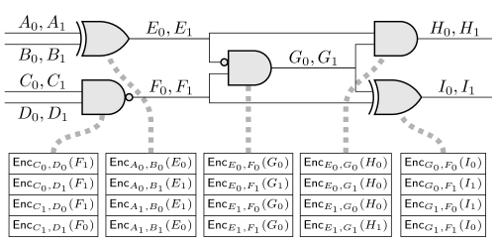
\includegraphics[width=1.0\textwidth]{Chapter2/Figs/Raster/garbledCircuit}
  \caption{Garbled Circuit example}
  \label{fig:garbledCircuit}
\end{figure}

Recent works provides optimizations to improve computation and communication
overhead associated with encrypt/decrypt operations and ciphertext tables'
sizes. In \cite{kolesnikov2008improved30}, the authors proposed a modification to
allow XOR gates to be evaluated \textit{for free}: the labels of XOR gates are
not chosen independently but by \(\omega_{i,0} = \omega_{i,1} \xor r\), for some
random value of \(r\). Pinkas et al. \cite{pinkas2009secure38} introduced a way to reduce communication size of binary gates by 25\%: each gate can be specified by three ciphertexts instead of all four. Finally, \cite{kolesnikov2009improved29} improve some commonly used circuits such as addition, comparision, etc. by reducing the number of non-XOR gates.

\subsection{Oblivious Transfer}
\label{sec:obliviousTransferPre}

\textit{"You take the blue pill, the story ends. You wake up in your bed and
  believe whatever you want to believe. You take the red pill, you stay in
  wonderland, and I show you how deep the rabbit hole goes."} - Morpheus to Neo,
the Matrix.


\begin{figure}[htbp!] 
\centering    
\includegraphics[width=1.0\textwidth]{Chapter2/Figs/Raster/RedPillBluePill}
\caption[Minion]{Red Pill - Blue Pill}
\label{fig:RedPillBluePill}
\end{figure}

What if, in such situation, there is a protocol to give privacy to
\(Neo\): \(Morpheus\) should not learn about \(Neo\)'s selection. Moreover, the
protocol can also provide privacy to \(Morpheus\): \(Neo\) should not learn
anything about the unchosen pill. In cryptography, Oblivious Transfer (OT) is a
protocol that can support such scenario. 
In the most basic form, it is a
two-parties protocol between a \textit{Sender} and a \textit{Receiver}, denoted
by \(\begin{psmallmatrix} 2 \\ 1 \end{psmallmatrix} \)-OT. The \(Sender\) uses
two private inputs \(x_{0}, x_{1}\) and the \(Receiver\) uses one input bit
\(s\). At the completion of the protocol, the \(Receiver\) gets the bit
\(x_{s}\) without letting the \(Sender\) know any information about the value of
\(s\): \(\begin{psmallmatrix} 2 \\ 1 \end{psmallmatrix}
\)-OT\((x_{0},x_{1};s) = x_{s}\).

The general idea is, when the receiver requests an item, the sender sends all the
items to the receiver and therefore it does not know which item is the one
requested. However, the response is encrypted in such a way that the receiver
can only decrypt the one he requested. A concrete implementation example of
\(\begin{psmallmatrix} 2 \\ 1 \end{psmallmatrix} \)-OT protocol based on
discrete log DH is illustrated in figure \ref{fig:DH21OT}. The receiver picks \(h_{0},h_{1}\) such that \(h_{0}h_{1} = h\), he cannot know both \(\log_{g}h_{0}\) and \(\log_{g}h_{1}\). Given \(h_{0}, h_{1}\), the sender returns ElGamal encryptions of bits \(x_{0}, x_{1}\) using \(h_{0},h_{1}\) as public keys. The receiver then decrypts one of the encryption to recover either \(x_{0} or x_{1}\)

\begin{figure}[h!]
  \centering
  \begin{equation*}
    \begin{array}{c c c}
      \text{\textbf{Sender}} & & \text{\textbf{Receiver}} \\
      \\
      (x_{0}, x_{1} \in \{0,1\}) & & (s \in \{0,1\}) \\
                             & & u \randomsample \mathbb{Z}_{n}\\
                             & & h_{s} \gets g^{u}\\
                             & & h_{1-s} \gets h/g^{u}\\
                             & \xleftarrow{h_{0}, h_{1}} & \\
      u_{0}, u_{1} \randomsample \mathbb{Z}_{n} & & \\
      (A_{0}, B_{0}) \gets (g^{u_{0}}, h_{0}^{u_{0}}g^{x_{0}}) & & \\
      (A_{1}, B_{1}) \gets (g^{u_{1}}, h_{1}^{u_{1}}g^{x_{1}}) & & \\
                             & \xrightarrow{(A_{0}, B_{0}),(A_{1}, B_{1})} & \\
      & & x_{s} \gets \log_{g}(B_{s}/A_{s}^{u})
    \end{array}
  \end{equation*}
  \caption{OT protocol based on DH}
  \label{fig:DH21OT}
\end{figure}

Efficient implementations of Oblivious Transfer can be found from \cite{naor2001efficient35}. The techniques from \cite{ishai2003extending24} can reduce a large number of OT protocol executions to \(\lambda\), where \(\lambda\) is the security parameter. In this thesis, we propose a new OT technique to be used with lattice-based cryptosystem.

\section{The Syntax and Security model}
\label{sec:syntaxModel}
We first describe the protocol and its security model in generic form.  We then can use them as a framework to apply and
analyze in our specific proposal.

% \subsubsection{Desirable properties}
% \label{sec:privacyProps}
% According to \cite{jain201650}, a secure template solution to biometric authentication should satisfy the following
% properties
% \begin{description}
% \item[Non-invertibility:] It is computationally hard to rebuild the original template from the encrypted one.
% \item[Non-linkability (Revocability):] It should be possible to revoke and to re-issue new encrypted templates using a
%   new key when the database is compromised.
% \item[Discriminability:] The secure scheme should not degrade the accuracy of the biometric authentication system.
% \end{description}
\subsubsection{The threats}
\label{sec:privacyReqs}
There are common security threats to many authentication systems such as Trojan horse, replay, man-in-the-middle (MITM)
attack, etc. Biometrics authentication systems are also vulnerable to such attacks. We can
borrow ideas from secure password-based schemes to address such issues. However, there are two categories of
vulnerabilities that are specific to biometric systems.  The first one is impersonation, or spoofing, the attack happens
at the client side where the adversary tries to cheat the system with counterfeit or invalid inputs.  The other issue is
at the server side with the privacy concern.

We will discuss the formal models that capture all the known threats of biometric authentication:
\begin{itemize}
\item Confidential data leakage due to attacks on the template database: Server breaches of biometric data always have
  catastrophic consequences (\cite{OPMsays563:online}), as we cannot change our fingerprints as easily as changing our
  passwords.
\item Hill-Climbing attack from the server side: This is also a privacy threat where the server trying to compute good
  inputs $X$ from the distance information between $X$ and $Y$ (\cite{uludag2004attacks}, \cite{higo2015privacy}). Note
  that Hill-Climbing attack by the client is very limited due to the limitation of the number of false authentication
  attempts in almost every biometric authentication system.
\item Impersonation by malicious client when the secret key of the user is known (replay attack): This happens when an
  attacker has access to the user's device but not his biometric, for example, in stolen device
  scenarios.(\cite{zhang2015fingerprints})
\item Impersonation by malicious client when the biometric template of the user is known (spoofing attack): This happens
  when an attacker collects biometric data and tries to reconstruct the template for authentication, for example,
  rebuilding the fingerprint from captured photos (\cite{zhang2015fingerprints},\cite{feng2011fingerprint}).
\item Cross matching of biometric data among databases: This threat uses information of the same user from different
  compromised databases to reconstruct the biometric template.
\end{itemize}

\subsubsection{The Generic Two-party model}

\begin{description}
\item[Entities:] There can be 2 or 3 typical entities involved in a secure biometric authentication system. The user
  $\mathcal{U}$, an authentication server $\mathcal{S}$, and a decryptor, who is a third party trusted by both of the
  users and the server. The decryptor presents in some systems (\cite{mandal2015comprehensive},
  \cite{hirano2013cryptographically}, \cite{higo2015privacy}), with the assumption that there is no collusion between
  this entity and $\user$ or $\server$. In our work, we aim to avoid the assumption of trusted decryptor party, so we
  only have two parties, $\user$ and $\server$.
\item[Biometrics Features in non-private setting] In biometric authentication systems (e.g., fingerprint authentication
  system), a user $\mathcal{U}$ first
  enrolls his fingerprint template $X$ with the server $\mathcal{S}$. $\mathcal{U}$ later authenticates with
  $\mathcal{S}$ using the same finger with a template $Y$, $\server$ uses an algorithm $Verify(X,Y)$ to obtain the
  result of the authentication: \textbf{Accept} or \textbf{Reject}. Different fingerprint system might use different
  features of fingers such as minutia or fingercode to compute this distance $\Delta$ between $X$ and $Y$ in the
  algorithm $Verify$. The distance $\Delta$ is compared to some predifined threshold value $\tau$ to determine the
  result of the authentication. We refer the reader to \cite{jain2007handbook} for biometric feature extraction and
  comparison techniques.\\

  Unlike password based system where $\user$ always uses one same query for many authentication, all biometric systems
  have the concept of False Acceptance Rate (FAR), where the system \textbf{Accept} an incorrect template; and False
  Rejection Rate (FRR), where the system \textbf{Reject} a genuine one.  Balancing these 2 rates while keeping good
  performances is one of the main challenges that fingerprint verification algorithms \cite{FVConGoi2:online} are trying
  to solve. We also reflect these two rates in our models.

\item[Algorithms and Procedures in privacy-preserving setting:] We describe the high level constructions of the protocol
  as follows
  \begin{description}
  \item[Enroll:] This procedure inserts records into the server's database.
    \begin{itemize}
    \item Input: Client: identity $k$, a registered template $X_k$; Server: Parameters of the cryptographic tools used.
    \item Output: A public-private key pair $(sk_k, pk_k)$ for the user $\user_k$. The server learns the protected
      template of $T_k$ of $X_k$.
    \end{itemize}
  \item[Auth:] This procedure allows a user to authenticate with the system.
    \begin{itemize}
    \item Input: Client: identity $k$, a query template $Y_k$ and the secret key $sk_k$; Server: record $(k, T_k, pk_k)$
    \item Output: The server learns the authentication result $res=\{\textbf{Accept,Reject}\}$
    \end{itemize}

  \item[Correctness Requirement:] A genuine user $\user_k$ does $(sk_k, T_k) \gets \mathbf{Enroll}(k, X_k)$ using a
    $X_k \in Supp(D_k)$ and later uses his biometric template $Y_k \randomsample D_k$ to do
    $$res \gets \mathbf{Auth}( (k, Y_k, sk_k), (k, T_k, pk_k))$$
    The privacy-preserving protocol works correctly if FRR under this system is exactly equal to FRR of the non-privacy
    preserving system:
    \[
      Pr[res = verify(X_k,Y_k)] = 1
    \]
  \end{description}
\end{description}

\subsubsection{The security model}
\begin{description}
\item[Privacy against an Honest But Curious server:] The security model is defined in terms of following security games.
  % Although the model assumes the server behaves honestly \emph{within} the protocol (since we our main aim is security
  % against passive exposure of server contents), it does allow the server to adversarially choose the client's
  % \emph{input} query templates $Y_i$ to try to learn about the attacked user's template $X_k$, so our model implies
  % security against `hill climbing attacks'~\cite{adler2005vulnerabilities}.

\item[The real game $\mathbf{Real}_{\attacker}(D_k,X_k)$:] This is the game for a privacy attack against the
  privacy-preserving protocol for the underlying biometric system, between an attacker $\attacker$ and a challenger
  $\challenger$. The input the game is an attacked $\user_k$ biometric distribution $D_k \in D_{bio}$ and a user
  template $X_k \in Supp(D_k)$.
  \begin{enumerate} %$\challenger$ selects a $\user_k$ with $D_k \in D_{bio}$ . For any $X_k \in Supp(D_k)$,
  \item $\challenger$ runs $(T_k, sk_k) \gets \mathbf{Enrol}(k,X_k)$ and sends $T_k$ to $\attacker$.
  \item For $i = 1 \dots q$:
    \begin{itemize}
    % \item $\attacker$ chooses and sends $Y_i$ to $\challenger$
    \item $\challenger$ samples \(Y_{i} \randomsample D_{k}\)
    \item $\challenger$ simulates the \textbf{Auth} protocol, playing the roles of both the client and the server:
      \[
        res \gets \mathbf{Auth_i}((k, Y_i, sk_k), (k, T_k, pk_k))
      \]
    \item Let $V_i$ denotes the $i^{th}$ view of $\server$ when $\challenger$ runs $\mathbf{Auth_i}$. $\challenger$
      sends the view $V_i$ to $\attacker$.
    \end{itemize}
  \item $\attacker$ outputs a bit $\beta$, representing some information that $\attacker$ has learned about
    $(D_k,X_k)$. The game output is $\mathbf{Real}_{\attacker}(D_k,X_k) = \beta$.
  \end{enumerate}

\item[The ideal game $\mathbf{Ideal}_{\attacker'}(D_k,X_k)$:] This is the game for a privacy attack against an ideal
  privacy scenario for the underlying biometric authentication system, where the attacker $\attacker'$ interacts with a
  challenger $\challenger'$. The input the game is an attacked $\user_k$ biometric distribution $D_k \in D_{bio}$ and a
  user template $X_k \in Supp(D_k)$. In this ideal game, the information $\attacker'$ can learn about $(D_k,X_k)$ is the
  value of \(HD_{X_{k}, Y_{k}}\) and the bit $Verify(X_k,Y_i)$.
  \begin{enumerate}
  \item For $i = 1 \dots q$:
    \begin{itemize}
    \item $\attacker'$ chooses query template $Y_i \in \{0,1\}^n$ and send it to $\challenger'$.
    % \item $\challenger'$ computes $res_i = verify(X_k, Y_i) \in \{\mathbf{Accept},\mathbf{Reject}\}$.
    \item $\challenger'$ sends $HD_{X,Y_{i}}$ to $\attacker'$.
    \end{itemize}
  \item $\attacker'$ output a bit $\beta'$, representing some information that $\attacker'$ has learned about
    $(D_k,X_k)$. The game output is $\mathbf{Ideal}_{\attacker'}(D_k,X_k) = \beta'$.
  \end{enumerate}
\end{description}
\begin{definition}
  [Privacy Security against Server] We say that a biometric authentication protocol is $q$-private in the sense of
  biometric template privacy against an honest but curious server $\server$ if for every efficient real-game attacker
  $\attacker$, there exists an efficient ideal-game attacker $\attacker'$ such that, for all $(D_k,X_k)$ we have:
  \[
    |\Pr[\mathbf{Real}_{\attacker}(D_k,X_k) = 1] - \Pr[\mathbf{Ideal}_{\attacker'}(D_k,X_k) = 1]| \leq negl(\lambda).
  \]
\end{definition}

\begin{description}
\item[Security against the malicious client:] In this work, we aim for security against active client, where an attacker
  $\attacker$ is assumed not to follow the protocol transcript.
  \begin{description}
  \item[Biometric Impersonation:] FAR is the usual biometric impersonation probability, it is inherent to the biometrics
    themselves without any cryptographic protocols. We first discuss this security game (which will be refered to as
    \textit{biometric impersonation}), then we elaborate the discussion to the models with privacy-preserving
    requirements.
    \begin{description}
    \item[Setup:] $\challenger$ samples $X_k \randomsample D_{k}$ from a random $\user_k$ ($D_k \randomsample D_{bio}$).
    \item[Query:] $\attacker$ is given access to the authentication oracle $verify(X_k,Y)$ that returns the
      authentication result of $\user_k$ with a query template $Y$. $\attacker$ has $q$ attempts to make queries, in
      each attempt, $\attacker$ chooses a $Y_{q}$ by himself and does $verify(X_k,Y_{q})$.
    \item[Guess:] $\attacker$ outputs $Y_{q'}$ such that $verify(X_k,Y_{q'}) = \textbf{Accept}$.
    \end{description}
    The advantage of $\attacker$ in the game is defined as
    \[
      \textbf{Adv}^{bio}_\attacker(\lambda) = Pr[verify(X_k,Y_{q'}) = \mathbf{Accept}]
    \]
    In this basic model, when $q=1$, the advantage of $\attacker$ is $FAR$.  In other words, we can say the advantage of
    $\attacker$ is $ \textbf{Adv}^{bio}_\attacker(\lambda) \leq q\times FAR$.

  \item[Privacy-Preserving Protocol:] This model extend the above protocol and captures the client side attacks
    mentioned in section \ref{sec:privacyReqs}.
    \begin{description}
    \item[Setup:] The setup phase includes 2 steps:
      \begin{itemize}
      \item $\challenger$ samples $X_k \randomsample D_{k}$ from a random $\user_k$ ($D_k \randomsample D_{bio}$).
      \item $\challenger$ runs $\textbf{Enroll}(k, X_k)$ that returns $(sk_k, T_k)$.
      \end{itemize}
    \item[Query:] In the query phase:
      \begin{itemize}
      \item $\attacker$ is given access to the authentication oracle $\mathbf{Auth}(Y)$ that returns the authentication
        result of $\user_k$ with a query template $Y$.
      \item $\attacker$ chooses the attack type $t \in \{I,II\}$ which specifies the scenario of key exposed or template
        exposed.

      \item $\challenger$ gives $sk_k$ if $t = I$ or $T_k$ if $t = II$ to $\attacker$. Note that, this model reflects
        the 2-factors authentication (the secret key and the biometric template), if $\attacker$ requests both factors,
        he loses the game.
      \item $\challenger$ and $\attacker$ runs $\mathbf{Auth()}$ $q$ times, For the $i^{th}$ run, $\attacker$ plays the
        client's role that chooses and sends $Y_i$ to $\challenger$, $\challenger$ plays the server's role that replies
        with $res_i = \mathbf{Auth}(Y_i)$.
      \end{itemize}
    \item[Guess:] $\attacker$ wins the game if it outputs $Y$ such that $\mathbf{Auth}(Y) = \textbf{Accepted}$.
    \end{description}
    The advantage of $\attacker$ in this game is defined as
    \[
      \textbf{Adv}^{Imp}_\attacker(\lambda) = Pr[\attacker \ wins] \
    \]
    We would want this advantage value not to be too large compared to the non-privacy-preserving biometric
    impersonation model's advantage $\textbf{Adv}^{bio}_\attacker(\lambda)$, which was bounded by $q \times FAR$.

  \end{description}

\end{description}
\begin{definition}
  [Impersonation Security] We say that a biometric authentication protocol is c-secure in the sense of template
  protection against the malicious user $\user$ if $\textbf{Adv}^{Imp}_\attacker(\lambda)$ is not greater than
  $\textbf{Adv}^{bio}_\attacker(\lambda)$ in some factor $c$ (if $c = 1$ we would have perfectly the same security level
  as the non-privacy-preserving system):
  \[\textbf{Adv}^{Imp}_\attacker(\lambda) \leq c \times \textbf{Adv}^{bio}_\attacker(\lambda)\]
\end{definition}


\section{Conclusion}
%%% Local Variables:
%%% mode: latex
%%% TeX-master: "../thesis"
%%% End:
%*******************************************************************************
%****************************** Second Chapter *********************************
%*******************************************************************************

\chapter{Security model}
\ifpdf
    \graphicspath{{Chapter3/Figs/Raster/}{Chapter3/Figs/PDF/}{Chapter3/Figs/}}
\else
    \graphicspath{{Chapter3/Figs/Vector/}{Chapter3/Figs/}}
\fi

\section{Introduction}
\label{sec:syntaxModel}
In this chapter, we first describe the protocol and its security model
generically.  We then go into details and further use it as a framework for our
specific proposals in later chapters. In order to precisely grasp the definition
of security, we will describe the protocols' security models in terms of
\textbf{attack games} played between two parties: a \textbf{challenger} and an
\textbf{adversary}, adapting the standard game based security model approach
commonly used in cryptography \cite{boneh2008graduate} . Generally, the
challenger \(\challenger\) follows a simple, fixed protocol and the adversary
\(\attacker\) may follow an arbitrary and efficient protocol. The two players
send messages back and forth to each other as specified in their protocols, and,
at the end of the games, \(\attacker\) outputs some value. We use
\textit{``simulation based''} security models, where the attack game defines a
probability space based on the output value , and it defines the adversary's
\textit{advantage}, which normally measures the difference between the
probabilities of two events in the given probability space: One is the event
that the adversary wins the \textit{real} game; the other one is the event that
a related adversary wins an ideal game with one (or some) of the system's
components replaced by an idealized version of such component(s). By
demonstrating that the advantage between the real and ideal games is negligible,
we can conclude that the security of the ``real'' protocol is essentially the
same as the ``ideal'' protocol. The security proofs of protocols will also be
organized as sequences of games. This technique appears in the literature in
different flavours with different degrees of formalisation. We also use an
incremental game based proof approach \cite{shoup2004sequences} as a helpful
tool to reduce the complexity of security proofs that might otherwise become
messy and complicated. We note that the technique is only a tool to organize the
models and the proofs, the actual ideas for cryptographic constructions and
security analysis come from elsewhere, specifically the problems discussed in
the previous chapter.

\subsection{Desirable properties}
\label{sec:privacyProps}
According to \cite{jain201650}, a secure template solution to biometric
authentication should satisfy the following properties:
\begin{description}
\item[Non-invertibility:] It is computationally hard to rebuild an original
  template from an encrypted one.
\item[Non-linkability (Revocability):] It should be possible to revoke and to
  re-issue new encrypted templates using a new key when the database is
  compromised.
\item[Discriminability:] The secure scheme should not degrade the accuracy of
  the biometric authentication system.
\end{description}
\subsection{The threats}
\label{sec:privacyReqs}
There are common security threats to many authentication systems such as Trojan
horse, replay, man-in-the-middle (MITM) attack. Biometrics authentication
systems are also vulnerable to such attacks. We can borrow ideas from secure
password-based schemes to address such issues. However, there are two categories
of vulnerabilities that are specific to biometric systems.  The first one is
impersonation, or spoofing. The attack happens at the client's side as the
adversary tries to cheat the system with counterfeit or invalid inputs.  The
other issue is at the server's side and yields privacy concerns.

We will present formal models that capture all the known threats of
biometric authentication:
\begin{itemize}
\item Confidential data leakage due to attacks on the template database: Server
  breaches of biometric data always have catastrophic consequences
  (\cite{OPMsays563:online}), as we cannot change our fingerprints as easily as
  changing our passwords.
\item Hill-Climbing attack from the server's side: This is a privacy threat
  where the server tries to compute good inputs $X$ from the distance
  information between $X$ and $Y$ (\cite{uludag2004attacks},
  \cite{higo2015privacy}). Note that Hill-Climbing attack by the client is very
  limited due to the limitation of the number of false authentication attempts
  in almost every biometric authentication system.
\item Impersonation by a malicious client when the secret key of the user is
  known (replay attack): This happens when an attacker has access to the user's
  device but not to his biometric data, as, for example, in stolen device
  scenarios (\cite{zhang2015fingerprints}).
\item Impersonation by a malicious client when the biometric template of the
  user is known (spoofing attack): This happens when an attacker collects
  biometric data and tries to reconstruct the template for authentication, as,
  for example, by rebuilding fingerprints from captured photos
  (\cite{zhang2015fingerprints},\cite{feng2011fingerprint}).
\item Cross matching of biometric data among databases: This threat uses
  information of the same user from different compromised databases to
  reconstruct the biometric template.
\end{itemize}

\section{The generic model}

\begin{description}
\item[Entities:] There can be 2 or 3 typical entities involved in a secure
  biometric authentication system. The user $\mathcal{U}$, an authentication
  server $\mathcal{S}$, and a decryptor, who is a third party trusted by both
  the user and the server. The decryptor appears in some systems
  (\cite{mandal2015comprehensive}, \cite{hirano2013cryptographically},
  \cite{higo2015privacy}), with the assumption that there is no collusion
  between this entity and $\user$ or $\server$. In our work, we avoid the
  assumption of a trusted decryptor party, so that only two parties are left:
  $\user$ and $\server$.
\item[Biometrics Features in non-private setting] In biometric authentication
  systems (e.g., fingerprint authentication system), a user $\mathcal{U}$ first
  registers his fingerprint template $X$ on the server
  $\mathcal{S}$. $\mathcal{U}$ later authenticates to $\mathcal{S}$ using
  the same finger with a template $Y$, $\server$ uses an algorithm $Verify(X,Y)$
  to obtain the result of the authentication: \textbf{Accept} or
  \textbf{Reject}. Different fingerprint systems might use different features of
  fingers such as minutia or fingercode \cite{ferrara2012noninvertible, jain1999fingercode} to compute the distance $\Delta$ between
  $X$ and $Y$ within the algorithm $Verify$. The distance $\Delta$ is compared
  to some predefined threshold value $\tau$ to determine the result of the
  authentication. We refer the reader to \cite{jain2007handbook} for biometric
  feature extraction and
  comparison techniques.

  Unlike password based systems, where $\user$ always uses one and the same
  query for many authentication trials, all biometric systems have the concept
  of False Acceptance Rate (FAR) (for the system \textbf{Accept}ing an incorrect
  template), and False Rejection Rate (FRR), (for the system \textbf{Reject}ing
  a genuine one).  As balancing these 2 rates while keeping good performances is
  one of the main challenges that fingerprint verification algorithms
  \cite{FVConGoi2:online} need to face, we also reflect these two rates in our
  models.

\item[Algorithms and Procedures in privacy-preserving settings:] We describe the
  high-level syntax of the privacy-preserving biometric authentication protocol consisting of the following procedures:
  \begin{description}
  \item[Enrol.] This procedure inserts records into the server's database.
    \begin{itemize}
    \item Client's input: identity $k$, a registered template $X_k$
    \item Server's input: Parameters of the cryptographic tools used.
    \item Output: A public-private key pair $(sk_k, pk_k)$ for the user
      $\user_k$. The server stores the protected biometric template $T_k$ (which is typically
      some encryption of $X_k$).
    \end{itemize}
  \item[Auth.] This procedure allows a user to authenticate to the system.
    \begin{itemize}
    \item Client's Input: identity $k$, a query template $Y_k$ and the secret key
      $sk_k$ 
    \item Server's Input: record $(k, T_k, pk_k)$
    \item Output: The server computes the authentication result
      $res=\{\textbf{Accept,Reject}\}$. The transcript of the protocol can also
      be obtained: We denote \(V_{c}\) and \(V_{s}\) to be the \textit{view} of
      the client and the server received from the protocol execution.
    \end{itemize}

  \item[Correctness Requirement:] A genuine user $\user_k$ executes
    $(sk_k, T_k) \gets \mathbf{Enroll}(k, X_k)$ using a $X_k \randomsample Supp(D_k)$ and
    later uses his biometric template $Y_k \randomsample D_k$ to perform
    $$res \gets \mathbf{Auth}_{\user,\server}( (k, Y_k, sk_k), (k, T_k, pk_k))$$
    Where $\user, \server$ are the honest client and server parties.
    The privacy-preserving protocol works correctly if the FRR under this system
    is exactly equal to the FRR of the non-privacy preserving system:
    \[
      Pr[res = verify(X_k,Y_k)] = 1
    \]
  \end{description}
\end{description}

\subsection{The privacy preserving model}
  Our security model intends to capture both threats for client and server's
  sides as discussed previously. There is only one variant which do not capture a
  threat related to Hamming Distance leakage to server, this imperfect privacy
  was introduced with the assumption that given such a value of HD of 2 bit
  strings, it is not feasible to infer information from the original bit
  strings.
\begin{description}
\item[Privacy against an Honest But Curious server:] The security model is defined in terms of the following security games.
  % Although the model assumes the server behaves honestly \emph{within} the protocol (since we our main aim is security
  % against passive exposure of server contents), it does allow the server to adversarially choose the client's
  % \emph{input} query templates $Y_i$ to try to learn about the attacked user's template $X_k$, so our model implies
  % security against `hill climbing attacks'~\cite{adler2005vulnerabilities}.

\item[The real game $\mathbf{Real}_{\attacker}(D_k,X_k)$:] This is the game for a privacy attack against the
  privacy-preserving protocol for the underlying biometric system, between an attacker $\attacker$ and a challenger
  $\challenger$. The input of the game is an attacked $\user_k$ biometric distribution $D_k \in D_{bio}$ and a user
  template $X_k \in Supp(D_k)$.
  \begin{enumerate} %$\challenger$ selects a $\user_k$ with $D_k \in D_{bio}$ . For any $X_k \in Supp(D_k)$,
  \item $\challenger$ runs $(T_k, sk_k) \gets \mathbf{Enrol}(k,X_k)$ and sends $T_k$ to $\attacker$.
  \item For $i = 1 \dots q$:
    \begin{itemize}
    % \item $\attacker$ chooses and sends $Y_i$ to $\challenger$
    \item $\challenger$ samples \(Y_{i} \randomsample D_{k}\)
    \item $\challenger$ simulates the \textbf{Auth} protocol, playing the roles of both the client and the server:
      \[
        res \gets \mathbf{Auth_i}((k, Y_i, sk_k), (k, T_k, pk_k))
      \]
    \item $\challenger$ sends the view $V_s^{i}$ to $\attacker$.
    \end{itemize}
  \item $\attacker$ outputs a bit $\beta$, representing some information that $\attacker$ has discovered about
    $(D_k,X_k)$. The game output is $\mathbf{Real}_{\attacker}(D_k,X_k) = \beta$.
  \end{enumerate}

\item[The ideal game $\mathbf{Ideal}_{\attacker'}(D_k,X_k)$:] This is the game for a privacy attack against an ideal
  privacy scenario for the underlying biometric authentication system, where an attacker $\attacker'$ interacts with a
  challenger $\challenger'$. The input of the game is an attacked $\user_k$ biometric distribution $D_k \in D_{bio}$ and a
  user template $X_k \in Supp(D_k)$. In this ideal game, the information $\attacker'$ can obtain about $(D_k,X_k)$ is the
  value of \(HD_{X_{k}, Y_{k}}\) and the bit $Verify(X_k,Y_i)$.
  \begin{enumerate}
  \item For $i = 1 \dots q$:
    \begin{itemize}
    \item $\attacker'$ chooses query template $Y_i \in \{0,1\}^n$ and sends it to $\challenger'$.
    % \item $\challenger'$ computes $res_i = verify(X_k, Y_i) \in \{\mathbf{Accept},\mathbf{Reject}\}$.
    \item $\challenger'$ sends $HD_{X,Y_{i}}$ to $\attacker'$.
    \end{itemize}
  \item $\attacker'$ output a bit $\beta'$, representing some information that
    $\attacker'$ has gathered about $(D_k,X_k)$. The game output is
    $\mathbf{Ideal}_{\attacker'}(D_k,X_k) = \beta'$.
  \end{enumerate}
\end{description}

Let \(W_{r}\) be the event that \(\attacker\) outputs $\beta = 1$ in the real game and let
\(W_{i}\) be the event that \(\attacker'\) output $\beta' = 1$ in the ideal game. We define
$\adv$'s \textbf{passive server security advantage} with respect to protocol $\pdv$ as
\[
\advantage{PS}{\adv,\pdv} = | Pr[W_{r}] - Pr[W_{i}]|
\]

\begin{definition}
  [Privacy Security against Server] We say that a biometric authentication
  protocol is $q$-private in the sense of biometric template privacy against an
  honest but curious server $\server$ if for every efficient real-game attacker
  $\attacker$, there exists an efficient ideal-game attacker $\attacker'$ such
  that, for all $(D_k,X_k)$, with $X_{k} \in Supp(D_{k})$, the following stands:
  \[
    \advantage{PS}{\adv,\pdv} \leq negl(n).
  \]
\end{definition}

Figure \ref{fig:passiveServerGame} and \ref{fig:passiveServerGameIdeal} show
schematic diagrams of the Privacy Security against Server games.

\begin{figure}[!h]
  \centering
  \begin{center}
    \begin{bbrenv}{PSGame}
      \begin{bbrbox}[name=Adversary, minheight=2cm]
        
      \end{bbrbox}
      \bbroutput{$\beta = A(T_{k}, (res_{i}, v_{s}^{i})_{i=1}^{q})$}
      \begin{bbrchallenger}{PSChallenger}
        \begin{bbrbox}[name=Challenger, minheight=2cm]
          \pseudocode{
            \\
            (\pk,\sk) \gets KeyGen\\
            % X_k \randomsample D_k\\
            T_k \gets \mathbf{enroll}(k,X_k)\\
            \text{For } i = 1,\dots,q:\\
            Y_k \randomsample D_k\\
            res_i = \mathbf{auth}(k,T_k,Y_k)
         } 
       \end{bbrbox}
       \bbrinput{$(X_k, D_k)$}
      \end{bbrchallenger}
      \bbrchallengerqryto{top=$T_{k}$}
      \bbrchallengerqryto{top=$res_{i}$}
      \bbrchallengerqryto{top=$V_{s}^{i}$}
      % \bbrchallengerqryto{top=$m_{2}$}
    \end{bbrenv}
  \end{center}
  \caption{Passive Server Attack Game (Real Game)}
  \label{fig:passiveServerGame}
\end{figure}

\begin{figure}[!h]
  \centering
  \begin{center}
    \begin{bbrenv}{PSGameIdeal}
      \begin{bbrbox}[name=Adversary, minheight=2cm]
        
      \end{bbrbox}
      \bbroutput{$\beta' = A'((res_{i})_{i=1}^{q})$}
      \begin{bbrchallenger}{PSChallengerIdeal}
        \begin{bbrbox}[name=Challenger]
          \pseudocode{
            \\
            (\pk,\sk) \gets KeyGen\\
            % X_k \randomsample D_k\\
            T_k \gets \mathbf{enroll}(k,X_k)\\
            \text{For } i = 1,\dots,q:\\
            Y_k \randomsample D_k\\
            res_i = Verify(X_k, Y_k)
         } 
        \end{bbrbox}
       \bbrinput{$(X_k, D_k)$}
      \end{bbrchallenger}
      % \bbrchallengerqryto{top=$T_{k}$}
      % \bbrchallengerqryto{top=$res_{i}$}
      \bbrchallengerqryto{top=$res_{i}$}
      % \bbrchallengerqryto{top=$m_{2}$}
    \end{bbrenv}
  \end{center}
  \caption{Passive Server Attack Game (Ideal Game)}
  \label{fig:passiveServerGameIdeal}
\end{figure}

At several points of this thesis, we will refer to the terms ``efficient'' and
``negligible'' (which will be defined formally in a section below). Intuitively,
\textit{negligible} means so small as to be ``zero for practical purposes''. For
example, consider an event happening with probability \(2^{-100}\): we would
not worry about such an event occurring more than we would worry about a similar
event occurring with probability 0. Additionally, an \textit{efficient
  adversary} is granted to run in a reasonable amount of time. Sometimes we
also use two other related terms: A value \(N\) is called \textit{super-poly} if
\(1/N\) negligible; and a \textit{poly-bounded} value is supposed to be a reasonably sized
number (we can say that the running time of any \textit{efficient} adversary is
a \textit{poly-bounded} value). We will use the results of the following lemma in
the security proofs:
\begin{lemma}
  If \(\epsilon\) and \(\epsilon'\) are negligible values, and \(Q\) and \(Q'\)
  are poly-bounded values, then
  \begin{itemize}
  \item \(\epsilon + \epsilon'\) is a negligible value
  \item \(Q + Q'\) and \(Q \cdot Q'\) are poly-bounded values
  \item \(Q \cdot \epsilon\) is a negligible value
  \end{itemize}
\end{lemma}

\begin{description}
\item[Security against a malicious client:] In this work, we aim at security
  against an active client, where an attacker $\attacker$ is assumed not to
  follow the protocol transcript.
  \begin{description}
  \item[Biometric Impersonation Attack Game.] FAR is the usual biometric
    impersonation probability, it is inherent to biometrics itself without any
    cryptographic protocols. We first discuss this security game (which will be
    referred to as \textit{biometric impersonation}), we then elaborate the
    discussion to account for models with privacy-preserving requirements.
    \begin{description}
    \item[Setup:] $\challenger$ samples $X_k \randomsample D_{k}$ from a random
      $\user_k$ ($D_k \randomsample D_{bio}$).
    \item[Query:] $\attacker$ is given access to the authentication oracle $q$ times
      $verify(X_k,Y_{i})$, which returns the authentication result of $\user_k$ with
      a query template $Y_{i}$. $\attacker$ has $q$ attempts to make queries, in
      each attempt, $\attacker$ chooses a $Y_{i}$ by himself and executes
      $verify(X_k,Y_{i})$.
    \item[Guess:] $\attacker$ outputs $Y_{q'}$ such that
      $verify(X_k,Y_{q'}) = \textbf{Accept}$.
    \end{description}

    Figure \ref{fig:maliciousNonPrivate} show the biometric
    impersonation (non private) attack game. Let $W_{0}$ be the event that there exists some $i$ such that
    $\attacker$ output $Y_{i}$ such that
    $verify(X_{k},Y_{i}) = \mathbf{Accept}$ and let $p_{0} = \prob{W_{0}} $.
    \begin{figure}[!h]
      \begin{center}
        \begin{bbrenv}{nonPrivacyServer}
          \begin{bbrbox}[name=Adversary, minheight=2cm]
            \pseudocode{
              \\
              \text{For } i = 1,\dots,q:\\
              Y_i \gets \{0,1\}^n
           } 
          \end{bbrbox}
          % \bbroutput{$Y_{q}'$}
          \begin{bbrchallenger}{nonPrivacyChallenger}
            \begin{bbrbox}[name=Challenger]
              \pseudocode{
                \\
                D_k \randomsample D_{bio}\\
                X_k \randomsample D_k\\
                res_i = Verify(X_k, Y_k)\\
              } 
            \end{bbrbox}
            \bbroutput{$(res_{1},\dots,res_{q})$}
          \end{bbrchallenger}
          \bbrchallengerqryfrom{top=$Y_{k}$}
          % \bbrchallengerqryto{top=$res_{i}$}
          \bbrchallengerqryto{top=$res_{i}$}
          % \bbrchallengerqryto{top=$m_{2}$}
        \end{bbrenv}
      \end{center}
      \caption{Malicious Client Attack Game in Non-private setting}
      \label{fig:maliciousNonPrivate}
    \end{figure}

    
    % The advantage of $\attacker$ in the game is defined as
    % \[
    %   \textbf{Adv}^{bio}_\attacker(\lambda) = Pr[verify(X_k,Y_{q'}) =
    %   \mathbf{Accept}]
    % \]
    % In this basic model, when $q=1$, the $p_{0} = FAR$.  In other words, we can
    % say the advantage of $\attacker$ is
    % $ \textbf{Adv}^{bio}_\attacker(\lambda) \leq q\times FAR$.

  \item[Impersonation Attack Game.] This game captures the basic impersonation attack from a client
    \begin{description}
    \item[Setup:] The setup phase includes 2 steps:
      \begin{itemize}
      \item $\challenger$ samples $X_k \randomsample D_{k}$ from a random
        $\user_k$ ($D_k \randomsample D_{bio}$).
      \item $\challenger$ runs $\textbf{Enroll}(k, X_k)$, which returns $(sk_k, pk_{k}, T_k)$.
      \end{itemize}
    \item[Query:] In the query phase:
      \begin{itemize}
      \item $\attacker$ is given access to the authentication oracle
        $\mathbf{Auth}$, the input to \textbf{Auth} supplied by $\attacker$ are
        the client's messages in the \textbf{Auth} protocol, returning the
        authentication result of $\user_k$ with a query template $Y$.

      \item $\challenger$ and $\attacker$ run $\mathbf{Auth()}$ $q$ times, For
        the $i^{th}$ run, $\attacker$ plays the client's role, $\challenger$ plays the server's role,
        replying with $res_i = \mathbf{Auth}$.
      \end{itemize}
    \item[Guess:] $\attacker$ wins the game if there exists $i$ such that $res_{i} = \textbf{Accepted}$.
    \end{description}
    Figure \ref{fig:impersonationAttackGame} show the impersonation attack
    game. Let $W_{1}$ be the event that there exists $i$ such that
    $res_{i} = \mathbf{Accepted}$ and let $p_{1} = \prob{W_{1}} $, recall that
    $P_{0}$ is the advantage of $\attacker$ in the biometric impersonation
    attack game. We define $\adv$'s \textbf{active impersonation advantage} with
    respect to the protocol $\pdv$ as
    \[
      \advantage{AI}{\adv,\pdv} = |p_{1} - p_{0}|
    \]
    \begin{definition}
      [Active Client Impersonation.] A privacy-preserving biometrics
      authentication protocol \pdv is c-secure against active client
      impersonation if for all efficient adversary \adv, the value
      $\advantage{AI}{\adv,\pdv}$ is not larger than $c \times FAR$ of the
      non-private protocol.
    \end{definition}
      
    \begin{figure}[!h]
      \begin{center}
        \begin{bbrenv}{impersonationSecurity}
          \begin{bbrbox}[name=Adversary, minheight=2cm]
            \pseudocode{
              \\
              \text{For } i = 1, \dots, q:\\
              Y_i \gets \{0,1\}^n
            }
          \end{bbrbox}
          % \bbroutput{$Y_{q}'$}
          \begin{bbrchallenger}{impersonationChallenger}
            \begin{bbrbox}[name=Challenger]
              \pseudocode{
                \\
                (\pk,\sk) \gets KeyGen\\
                D_k \randomsample D_{bio}\\
                X_k \randomsample D_k\\
                T_k \gets \mathbf{enroll}(k,X_k)\\
                res_i = \mathbf{Auth}(Y_i, T_k, k)
              } 
            \end{bbrbox}
            \bbroutput{$(res_{1}, \dots, res_{q})$}
          \end{bbrchallenger}
          \bbrchallengerqryto{top=$pk_{k}$}
          \bbrchallengerqryfrom{top=$Auth_{i}$}
          \bbrchallengerqryto{top=$V_c^i$}
          \bbrchallengerqryto{top=$res_{i}$}
          % \bbrchallengerqryto{top=$m_{2}$}
        \end{bbrenv}
      \end{center}
      \caption{Impersonation Attack Game}
      \label{fig:impersonationAttackGame}
    \end{figure}


  \item[Multifactor Attack Game.] This model extends the above protocol and
    captures the client side attacks mentioned in section \ref{sec:privacyReqs}.
    \begin{description}
    \item[Setup:] The setup phase includes 2 steps:
      \begin{itemize}
      \item $\challenger$ samples $X_k \randomsample D_{k}$ from a random
        $\user_k$ ($D_k \randomsample D_{bio}$).
      \item $\challenger$ runs $\textbf{Enroll}(k, X_k)$, which returns $(sk_k, T_k)$.
      \end{itemize}
    \item[Query:] In the query phase:
      \begin{itemize}
      \item $\attacker$ chooses the attack type $t \in \{I,II\}$ which specifies
        the scenario of key exposure or template exposure.

      \item $\challenger$ passes $sk_k$ if $t = I$ or $T_k$ if $t = II$ to
        $\attacker$. Note that this model reflects the 2-factors authentication
        (the secret key and the biometric template), and, thus, if $\attacker$
        requests both factors, he loses the game.
      % \item $\attacker$ is given access to the authentication oracle
      %   $\mathbf{Auth}(Y)$ returning the authentication result of $\user_k$ with
      %   a query template $Y$.
      \item $\challenger$ and $\attacker$ run $\mathbf{Auth()}$ $q$ times, For
        the $i^{th}$ run, $\attacker$ plays the client's role, choosing and
        sending $Y_i$ to $\challenger$, $\challenger$ plays the server's role,
        replying with $res_i = \mathbf{Auth}(Y_i)$.
      \end{itemize}
    \item[Guess:] $\attacker$ wins the game if it outputs $Y$ such that
      $\mathbf{Auth}(Y) = \textbf{Accepted}$.
    \end{description}
    
    Figure \ref{fig:multifactorAttackGame} show the multi-factors attack
    game. Let $W_{2}$ be the event that there exists $i$ such that
    $res_{i} = \mathbf{Accepted}$ and let $p_{2} = \prob{W_{2}} $. Let $p_{0}$
    define the winning probability of the $\attacker$ in the non-privacy
    biometric authentication game. We define $\adv$'s \textbf{active multifactor
      advantage} with respect to the protocol $\pdv$ as
    \[
      \advantage{AM}{\adv,\pdv} = |p_{2} - p_{0}|
    \]
    
    \begin{figure}[!h]
      \begin{center}
        \begin{bbrenv}{multifactorSecurity}
          \begin{bbrbox}[name=Adversary, minheight=3cm]
            \pseudocode{
              \\
              type \gets \{I,II\}\\
              \text{For } i = 1, \dots, q:\\
              Y_i \gets \{0,1\}^n
            }
          \end{bbrbox}
          % \bbroutput{$Y_{q}'$}
          \begin{bbrchallenger}{multifactorChallenger}
            \begin{bbrbox}[name=Challenger, minheight=2cm]
              \pseudocode{
                \\
                (\pk,\sk) \gets KeyGen\\
                D_k \randomsample D_{bio}\\
                X_k \randomsample D_k\\
                T_k \gets \mathbf{enroll}(k,X_k)\\
                res_i = \mathbf{Auth}(Y_i, T_k, k)
              } 
            \end{bbrbox}
            \bbroutput{$(res_{1},\dots,res_{q})$}
          \end{bbrchallenger}
          \bbrchallengerqryto{top=$pk_{k}$}
          \bbrchallengerqryfrom{top=type I,bottom=or II}
          \bbrchallengerqryto{top=$sk$,bottom=or $D_{k}$}
          \bbrchallengerqryfrom{top=$Auth_{i}$}
          \bbrchallengerqryto{top=$V_c^i$}
          \bbrchallengerqryto{top=$res_{i}$}
          % \bbrchallengerqryto{top=$m_{2}$}
        \end{bbrenv}
      \end{center}
      \caption{Multi-factors Attack Game}
      \label{fig:multifactorAttackGame}
    \end{figure}
    
    Similar to the previous impersonation attack game, We would want this
    advantage value not to be too large compared to the non-privacy-preserving
    biometric impersonation model's advantage, which was bounded by
    $q \times FAR$.
  \end{description}

\end{description}
\begin{definition}
  [Active Multi-factors.] A privacy-preserving biometrics authentication
  protocol $\pdv$ is c-secure against active multi-factors attack if for all
  efficient adversary $\adv$, the value $\advantage{AM}{\adv,\pdv}$ is not
  larger than $c \times FAR$ of the non-private protocol.
\end{definition}

\section{Security Proof Technique}
In the security proofs of the protocols appearing in the next chapters, we will typically
model the security games following the generic framework defined in this
chapter, with the \textbf{Enroll} and \textbf{Auth} modules replaced by concrete
lattice-based constructions (or combination of them). Each attack game is
modeled by way of a probability space, as both \textit{adversary} and
\textit{challenger} are probabilistic processes communicating with each other. The
definition of security is tied to some particular event S as seen in previous
sections (where security means that for all \textit{efficient} adversary, the
probability that event S happens is \textit{close to} some target probability,
normally \textit{negligibly} small, 1/2, or FAR in one of our contexts). In
formal definitions, there is a security parameter related to the terms
\textit{efficient} or \textit{negligible}. For example, \textit{efficient} means
time bounded by a polynomial in the security parameter, \textit{close to} means
the difference is smaller than inverse of any polynomial in the security
parameter. For simplicity, we assume that all algorithms, adversaries,
challengers, etc., take this parameter value as an implicit input.

The approach used in the security proofs is called \textit{sequence-of-games},
the process is as follows. In each proof,  a sequence of games is set up:
Game 0, Game 1, \dots, Game $n$, where Game 0 is normally the original attack
game with respect to a concrete protocol and a given adversary. Let $S_{0}$ be
the event S. For i=1,\dots,n, the construction defines an event $S_{i}$ for each
Game $i$, these events are normally related to S in a natural way. Then, the
proof shows that $\prob{S_{i}}$ is \textit{close to} $\prob{S_{i+1}}$ for all
$i=0,\dots,n-1$. Finally, if $\prob{S_{n}}$ can be shown to be \textit{close to}
the ``target probability'', provided that $n$ is a constant, we can infer that
$\prob{S}$ is negligibly close to the ``target probability'', and security is
proved. We have ensured that the changes from one game $i$ to the next game
$i+1$ are kept as small as to avoid major complications while analyzing them.

Generally, there are two types of changes in the proofs:
\begin{description}
\item[Change based on indistinguishability] A change is made such that its detection by the adversary implies a method of distinguishing two
  distributions that are statistically or computationally indistinguishable. For
  instance, if $P_{1}$ and $P_{2}$ are two indistinguishable distributions,
  to prove that $|\prob{S_{i}} - \prob{S_{i+1}}|$ is negligible, it should be shown
  that there exists an algorithm $D$ such that, when inputting an
  element drawn from $P_{1}$, outputs 1 with probability $\prob{S_{i}}$; and
  when inputting an element drawn from $P_{2}$, outputs 1 with
  probability $\prob{S_{i+1}}$. It follows that
  $|\prob{S_{i}} - \prob{S_{i+1}}|$ is negligible, provided the
  indistinguishability assumption of $P_{1}$ and $P_{2}$.
\item[Change based on failure events] This type of change is based on the fact
  that, given $A,B,F$ as events in some distribution, and supposing that
  $A \wedge \neg F \iff B \wedge \neg F$, then
  $|\prob{A} - \prob{B}| \leq \prob{F}$, to say that two games proceed
  identically unless F occurs, means that $S_{i} \wedge \neg F$ and
  $S_{i+1} \wedge \neg F$ are the same. So, in order to prove that $\prob{S_{i}}$ is
  negligibly close to $\prob{S_{i+1}}$, it is enough to prove that $\prob{F}$ is
  negligible. This can be done using the security assumption or an
  information-theoretic argument, as, for instance, that when F occurs, the adversary
  could find a collision in a cryptographic hash function.
\end{description}

\subsection{Related work}
\label{sec:proofRelatedWork}

Sequence of transitions based on indistinguishability (only) have been used
extensively in cryptography for many years. For example, in 1984,
\cite{goldreich1984construct} illustrated the ``hybrid arguments'' technique while
constructing pseudo-random functions. \cite{bellare1989new} was an early example
of a proof that is structured as a sequence of games including transitions based
on both failure events and indistinguishability. The first formal approach to
sequences of games was initiated by Kilian and Rogaway's paper
\cite{kilian1996protect}. The authors subsequently applied the technique in
numerous papers, detailed introduction to the methodology and references of usage
can be found in \cite{bellare2004game}. In Bellare and Rogaway's approach, games
are treated as syntactic objects subject to formal manipulation, while
\cite{shoup2004sequences} views games as probability spaces with random variables
defined over them. This proof style is also illustrated nicely by some public
key cryptography examples in an introductory manuscript
\cite{pointcheval2005provable}. The technique has been used widely
(\cite{abdalla2005password}, \cite{boneh2005improved}, \cite{bresson2002group},
etc. ). While some of the proofs can be structured differently,
sequence-of-games is a technique able of accomplishing the task in a clear and
convincing way.

\section{Conclusion}
This chapter lays out the framework to be used as the security models and hints at the way
security proofs will be organized. The technique (sequence-of-games) will
be used subsequently in the next chapters within each of the protocol variants to
illustrate to illustrate correspondingly security properties. 
%%% Local Variables:
%%% mode: latex
%%% TeX-master: "../thesis"
%%% End:
\chapter{The Second Protocol - Covering Circuit Privacy}
\label{chap:renyiDivergence}

% **************************** Define Graphics Path **************************
\ifpdf
    \graphicspath{{Chapter4/Figs/Raster/}{Chapter4/Figs/PDF/}{Chapter4/Figs/}}
\else
    \graphicspath{{Chapter4/Figs/Vector/}{Chapter4/Figs/}}
\fi

\section{Introduction}
\label{sec:secProcIntro}
This chapter discusses Circuit Privacy, which is an important aspect of
Homomorphic Encryption, and how it affects the security of our first variant
of the protocol. We also describe a new technique being used to improve the
security proof of the protocol, to make sure that we can choose parameters small
enough for the system for practical reasons, but still preserve the security level. In
particular, we show how to use the infinity-order Renyi Divergence (RD) instead of
traditional Statistical Distance in the proof, in order to significantly lower the initial noise bound parameter, which will result in a smaller moduli \(q\) for the ring \(R_{q}\) used by the
cryptosystem.

Circuit Privacy means that the ciphertext generated by a homomorphic operation
does not reveal anything about the circuit it evaluates, except its output
value. This property applies even to the party having generated the
keys.

Consider a ciphertext product result in a BV cryptosystem (section
\ref{sec:BVScheme}).
\[
  mult(c,c') = (\mathbf{c_0}\mathbf{c_0'}, \mathbf{c_0}\mathbf{c_1'} +
  \mathbf{c_1}\mathbf{c_0'}, \mathbf{c_1}\mathbf{c_1'})
\]
The noise term of this result ciphertext correlates to both $\mathbf{s}$ and $\mathbf{m}$.
In many contexts, a leakage of this kind might be inconsequential for a genuine user with a secret key, because s/he is supposed to know the key and decrypt the message.
However, in many other contexts, especially in multi-factor authentication
scenarios, this is not the case. For instance, in our system, we do not want the
client to know the Hamming Distance value, so that an attacker with a stolen
device and a secret key cannot derive information about the data stored in the
server from the enrolment stage?. We propose to mask this data by homomorphically adding the ciphertext
$Enc(HD)$ to $Enc(r)$ so as to refresh the noise terms while masking the Hamming Distance at the same time. The question is how far from the original noise distribution we can move away without compromising correctness, if this new security measure is applied.

Let $D_1$ and $D_2$ be the probability distributions of the original noise in the ciphertext $Enc(HD)$ and the new shifted noise of $Enc(HD+r)$. We observe that the
2 Gaussian distributions are identical with the same standard deviation
$\sigma$ and different means. Let $r_0$ be the shift in the means of $D_1$ and $D_2$.
Our goal is to set up parameter $r_0$, such that $D_1$ and $D_2$ are computationally
indistinguishable while keeping other parameters of the cryptosystem within practical
performance
thresholds. Statistical Distance (SD) is normally used to measure the difference of distributions and is generally bound by
\[
SD(D_1, D_2) = \frac{1}{2}\sum_{x\in X}|D_1(x) - D_2(x)| \leq K\times \frac{r_0}
{\sigma}
\]
where $K$ is a constant. We quickly see that in order for $SD$ to be indistinguishable, ($SD < \epsilon \approx \frac{1}{2^\lambda}$, where $\lambda$ is
the security parameter), the standard deviation of the initial noise needs to be really large, that is $\sigma \geq Kr_02^\lambda$.

In the work of \cite{bai2015improved}, the authors proposed Renyi Divergence (RD) as
an alternative to measure distributions' closeness and its applications to security proofs. $R_a(D_1\|D_2)$ of order $a$
between $D_1$ and $D_2$ is defined as the expected value of $(D_1(x)/D_2(x))^{a-1}$ over the randomness of $x$, sampled from $D_1$.
\[
R_a(D_1\|D_2) = \left( \sum_{x \in D_1}\frac{D_1(x)^a}{D_2(x)^{a-1}} \right)^
{\frac{1}{a-1}}
\]
Similar to SD, RD is useful in our context with its \textit{Probability Preservation} property (we refer readers to \cite{bai2015improved} for detailed formal
descriptions): Given $D_1$ and $D_2$ as described, for any event $E$, for instance, we want to verify that $P(E)$ is the winning probability of the attacker in the distinguishing game, the probability of the event with respect to $D_2$ being bound by
\begin{align}
\label{eq:renyi}
D_2(E) \geq D_1(E)^{\frac{a}{a-1}}/RD_a(D1\|D_2)
\end{align}
Particularly, if we look at the second order ($a = 2$) of RD as done in previous
works, we would have $ D_2(E) \geq D_1(E)^2/RD_2(D1\|D_2) $.  Provided that the
distribution functions on lattices of $D_1$ and $D_2$ are discrete Gaussian,
which is of the form
$\rho_\sigma(x) = \frac{1}{\sigma}e^{-\pi\frac{x^2} {\sigma^2}}$ ,
$RD_2(D_1\|D_2) = e^{2\pi \frac{r_0^2}{\sigma^2}} \approx e^{2\pi}$, when $r_0$
is much smaller than $\sigma$. This means that when switching from $D_1$ to $D_2$,
the success probability of $E$ will be at least the old probability to the power
of 2 divided by some constant. This squaring factor brings about a big trade-off: for
example, in our protocol, we would need to use $FAR = 2^{-20}$ in the
non-privacy biometric settings to get $FAR=2^{-10}$ into our scheme.

We aim at a solution to remove this factor. The idea is to look at $RD_\infty$
instead of at $RD_2$: from equation (\ref{eq:renyi}), we can infer that when $a$ is
large, $\frac{a}{a-1}$ becomes 1. However, for usual Gaussian distributions, the value of
$RD_\infty$ is also infinity (not a constant $e^{2\pi}$ like in $RD_2$ when
$a=2$). This is due to the ratios $\frac{D_1(x)}{D_2(x)}$, which become large when
samplings are done in the extreme tails of the distributions. Our idea is to
truncate the distribution when doing noise sampling: if we get a noise value
that is too close to the tail, we reject it and sample again. As a result, the
truncated distribution grows slightly, that means, the small noises show
higher probability when sampling, which does not have a high impact on security.


\section{Context and Related Work}
\label{sec:secProcPrevious}

\subsection{Definitions}
\label{sec:renyiDefinition}

\subsubsection{Circuit Privacy}
\label{sec:renyiCircuitPrivacy}

To define Circuit Privacy, we view the operation of \(Evaluate\) (Section
\ref{sec:defHomo}) as a protocol between a client who generates the keys and
encrypts the input, and a server who evaluates some function on that input and
returns the result to the client.

\begin{definition}
  [Circuit privacy.] A homomorphic encryption scheme E = (KeyGen,
  Encrypt, Decrypt, Evaluate), correct for the circuit family C, is circuit
  private for C, if there exists an efficient simulator Sim such that, for every
  \(\tau \in \mathbb{N}, \pi \in C_{\tau},\) and plaintext bits \textbf{b} =
  \((b_{1}, \dots, b_{t}) \in \{0,1\}^{t}\), one for every input bit of \(\pi\),
  we have\\
  $$Real_{\pi,\mathbf{b}}(\lambda) \approx Sim(1^{\lambda}, 1^{\tau},
  \mathbf{b}, \pi(\mathbf{b}))$$ Where\\
  \(Real_{\pi,\mathbf{b}}(\lambda) = \{(r,r',c): r, r' \randomsample \$, (sk,
  pk) \gets KeyGen(1^{\lambda}, 1^{\tau}, r), c \gets Encrypt(pk, \mathbb{b},
  r'), c' \gets Evaluate(pk, \pi, \mathbf{c})\}\)
\end{definition}
We note that the simulator \(Sim\) is given the output \(\pi(\mathbf{b})\) but
not the description of the circuit \(\pi\) itself, and it needs to simulate the
view that includes the randomness from key generation, encryption and
ciphertext evaluation operations

\subsubsection{Renyi Divergence}
\label{sec:renyisubdefinition}
\begin{definition}
  [Renyi Divergence] Let \(Supp(D) = \{x: D(x) \neq 0\}\) denotes the
  \textit{support} for a probability distribution \(D\). For any two discrete
  probability distributions \(P\) and \(Q\) such that
  \(Supp(P) \subseteq Supp(Q)\) and \(a \in (1, +\infty)\), the Renyi divergence
  of order a is defined by\\
  $$RD_{a} = \left(\sum_{x \in Supp(p)}\frac{P(x)^{a}}{Q(x)^{a-1}}\right)^{\frac{1}{a-1}}$$
\end{definition}
When \(a = 2\), the subscript is normally omitted, the Renyi divergence of
order \(+\infty\) is defined by
\(RD_{\infty} = max_{x \in Supp(P)}\frac{P(x)}{Q(x)}\). The definitions are
extended in the natural way to continuous distributions. The following
properties are considered analogues of those of Statistical Distance. Proofs can
be found in \cite{langlois2014gghlite}.
\begin{lemma}
  Let \(a \in [1, +\infty]\). Let \(P\) and \(Q\) denote distributions with
  \(Supp(P) \subseteq Supp(Q)\). Then the following properties hold:
  \begin{description}
  \item [Log. Positivity.] \(RD_{a}(P || Q) \geq RD_{a}(P||P) = 1\).
  \item[Data Processing Inequality]
    \(RD_{a}(P^{f} || Q^{f}) \leq RD_{a}(P || Q)\) for any function \(f\), where
    \(P^{f}\) and \(Q^{f}\) denote the distribution of \(f(y)\) induced by
    sampling \(y \randomsample P\) and \(y \randomsample Q\)
  \item[Multiplicative] Assume \(P\) and \(Q\) are two distributions of a pair
    of random variables \((Y_{1}, Y_{2})\). For \(i \in \{1,2\}\), let \(P_{i}\)
    and \(Q_{i}\) denote the marginal distribution of \(Y_{i}\) under \(P\) and
    \(Q\), and let \(P_{2|1}(\cdot | y_{1})\) and \(Q_{2|1}(\cdot | y_{1})\)
    denote the conditional distribution of \(Y_{2}\) given that
    \(Y_{1} = y_{1}\). Consequently:
    \begin{itemize}
    \item \(RD_{a}(P||Q) = RD_{a}(P_{1}||Q_{1}) \cdot RD_{a}(P_{2}||Q_{2}))\) if
    \(Y_{1}\) and \(Y_{2}\) are independent for \(a \in [1,\infty]\).
    \item
    \(RD_{a}(P||Q) \leq RD_{\infty}(P_{1} || Q_{1}) \cdot max_{y_{1} \in X}
    RD_{a}(P_{2|1}(\cdot | y_{1})||Q_{2|1}(\cdot | y_{1}))\)
    \end{itemize}
  \item[Probability Preservation] Let \(E \subseteq Supp(Q)\) be an arbitrary
    event. If \(a \in (1, +\infty)\), then
    \(Q(E) \geq P(E)^{\frac{a}{a-1}}/RD_{a}(P||Q)\) and
    \(Q(E) \geq P(E)/RD_{\infty}(P||Q)\)
  \item[Weak Triangle Inequality] Let \(P_{1}, P_{2}, P_{3}\) be three
    distributions with
    \(Supp(P_{1}) \subseteq Supp(P_{2}) \subseteq Supp(P_{3})\). Consequently:\\
    \(RD_{a}(P_{1}||P_{3}) \leq
    \begin{cases}
      RD_{a}(P_{1}||P_{2}) \cdot R_{\infty}(P_{2}||P_{3}),\\
      RD_{\infty}(P_{1}||P_{2})^{\frac{a}{a-1}} \cdot RD_{a}(P_{2}||P_{3})
      \text{if } a \in (1,+\infty)
    \end{cases}
\)
  \end{description}
\end{lemma}

\subsection{Related Work}
\label{sec:renyiRelatedWorks}
Ling et al. \cite{ling2017hardness} used RD as the framework for distinguishing
problems in the \textit{k}-LWE context, which is a variant of LWE in which the
adversary is given extra information in the distinguishing attack game. The
work of \cite{poppelmann2014enhanced27} used RD order 1 (Kullback-Leibler
divergence) to improve the communication size requirement of BLISS
\cite{ducas2013lattice11}. \cite{bai2015improved5} showed how generic RD can
be used as an alternative to the statistical distance in proofs for
lattice-based cryptography.  Bogdanove et al. \cite{bogdanov2016hardness4}
adapted the work of \cite{bai2015improved5} to the Learning With Rounding
problem. RD was used in \cite{libert2016signature} in the context of dynamic
group signatures and also in \cite{alkim2016post} to replace LWE noise
distribution by an easier to sample distribution.


\section{Renyi Divergence Analysis technique}
\label{sec:secProcRenyi}
% \subsection{Renyi Divergence and its application in noise masking}
% \label{sec:Renyi_original}

For the following analysis, let $D_1$ be a discrete Gaussian on $\mZ$ with
deviation parameter $\sigma$ shifted by the constant $r_0 \in \mZ$, while $D_2$
is a discrete Gaussian on $\mZ$ with dev. par. $\sigma$ centered on zero,
i.e. $D_1 = D_{\mZ,\sigma} + r_0$ and $D_2 = D_{\mZ,\sigma}$, where
$D_{\mZ,\sigma}(x) = e^{-\pi \cdot x^2/\sigma^2}/\sum_{z \in \mZ} e^{-\pi \cdot
  z^2/\sigma^2}$ for $x \in \mZ$. To allow us to use $RD_{\infty}$ we put
tail-cut variants $D_1^{(cut)}$ and $D_2^{(cut)}$ of $D_1$ and $D_2$ into play,
respectively with parameter $k$. The parameter $k$ defines where $D_1$ and $D_2$
are cut, for example, we can set $k=3$ to cut the distributions at 3
deviation parameters from the mean. So, we let $D_{\mZ,\sigma}^{(cut)}$ denote
distribution $D_{\mZ,\sigma}$ tail-cut to the interval
$[-k \cdot \sigma, k \cdot \sigma]$ by rejection sampling. We let
$D_1^{(cut)} = D_{\mZ,\sigma}^{(cut)} + r_0$ and
$D_2^{(cut)} = D_{\mZ,\sigma}^{(cut)}$. Notice that the supports of
$D_1^{(cut)}$ and $D_2^{(cut)}$ are different, namely
$Supp(D_1^{(cut)}) = [-k\sigma+r_0,k\sigma+r_0]$ while
$Supp(D_2^{(cut)}) = [-k\sigma,k\sigma]$. We assume, without loss of generality,
that $r_0 > 0$. We would like to switch from distribution $D_1^{(cut)}$ to
$D_2^{(cut)}$, but unfortunately $R_\infty(\overline{D}_1^{(cut)}\|D_2^{(cut)})$
is not finite, since $Supp(D_1^{(cut)})$ is not a subset of
$Supp(D_2^{(cut)})$. To satisfy the latter condition, we first switch from
$D_1^{(cut)}$ to $\overline{D}_1^{(cut)}$ by further cutting (by rejection
sampling) the positive tail of $D_1^{(cut)}$ to ensure it does not go beyond the
$k \sigma$ upper bound on tail of $D_2^{(cut)}$, and use a (mild condition)
statistical distance step to lower bound $\overline{D}_1^{(cut)}(E)$. Then, in a
second step using
$Supp(\overline{D}_1^{(cut)})=[-k\sigma+r_0, k\sigma] \subseteq
[-k\sigma,k\sigma] = Supp(D_2^{(cut)})$, we derive a finite upper bound on
$R_\infty(\overline{D}_1^{(cut)}\|D_2^{(cut)})$ to lower bound
$D_2^{(cut)}(E)$. Details follow.
\begin{sloppypar}
  \textbf{First SD Step.} Since $Supp(D_1^{(cut)})$ is transformed into
  $\overline{D}_1^{(cut)}$ by rejection and resampling if a sample of
  $Supp(D_1^{(cut)})$ falls in $(k\sigma,k\sigma+r_0]$, we have
  $SD(D_1^{(cut)}, \overline{D}_1^{(cut)}) \leq
  D_1^{(cut)}((k\sigma,k\sigma+r_0]) = D_2^{(cut)}((k\sigma-r_0,k\sigma]) =
  D_{\mZ,\sigma}((k\sigma-r_0,k\sigma])/C_2$, where
  $C_2 = D_{\mZ,\sigma}([-k\sigma,k\sigma])$. Consequently,
$$
\Delta \defeq \frac{D_{\mZ,\sigma}((k\sigma-r_0,k\sigma])}{C_2} = \frac{\sum_{z
    \in (k\sigma-r_0,k\sigma])} \e^{-\pi z^2/\sigma^2}}{\sum_{z \in
    [-k\sigma,k\sigma])} \e^{-\pi z^2/\sigma^2}}.
$$
For the numerator, the upper bound
$\sum_{z \in (k\sigma-r_0,k\sigma])} \e^{-\pi z^2/\sigma^2} \leq
\int^{\infty}_{k\sigma-r_0} \e^{-\pi z^2/\sigma^2} dz \leq \sigma \cdot \e^{-\pi
  (k\sigma-r_0)^2/\sigma^2}$ is obtained by using the standard normal distribution upper bound
$\int^{\infty}_{\gamma} \frac{1}{\sqrt{2\pi} \sigma} \cdot \e^{- z^2/\sigma^2}
dz \leq \e^{-\gamma^2/(2\sigma^2)}$ for $\gamma \geq 0$. For the denominator, the lower bound is
$\sum_{z \in [-k\sigma,k\sigma]} \e^{-\pi z^2/\sigma^2} \geq 2 \cdot \sum_{z \in
  [0,k\sigma])} \e^{-\pi z^2/\sigma^2} \geq 2 \cdot (\int^{\infty}_{0} \e^{-\pi
  z^2/\sigma^2} dz - \int^{\infty}_{k\sigma} \e^{-\pi z^2/\sigma^2} dz) \geq
\sigma \cdot (1 - 2 \cdot \e^{-\pi (k\sigma-r_0)^2/\sigma^2})$. Therefore,
$SD(D_1^{(cut)}, \overline{D}_1^{(cut)}) \leq \Delta \leq \delta' / (1-2\delta')
\leq 2\delta'$ if $\delta' \leq 1/4$, where
$\delta' = \e^{-\pi (k\sigma-r_0)^2/\sigma^2}$. Defining $\delta = 2\delta'$, makes $\Delta \leq \delta$ if $\delta \leq 1/8$ and the conditions
$r_0 \leq \sigma$ and $k \geq 1 + \sqrt{1/\pi \cdot \ln(2/\delta)}$
hold. Therefore, for any event $E$, 
$\overline{D}_1^{(cut)}(E) \geq D_1^{(cut)}(E) - \delta$ is the case.
\end{sloppypar}
% with probability $D_1^{(cut)}(E)$ \geq \varepsilon$, we have can take $\delta
% = \var{\epsilon This tells us how to set the tail cut parameter $k$.

\textbf{Second RD step.} The desired RD of order $\infty$ is defined by
\[
  R_\infty(\overline{D}_1^{(cut)}\|D_2^{(cut)})) = \max_{x \in
    [-k\sigma+r_0,k\sigma]} \frac{\overline{D}_1^{(cut)}} {D_2^{(cut)}(x)}.
\]
Observe that, for each $x \in [-k\sigma+r_0,k\sigma]$, we have
$\overline{D}_1^{(cut)}(x) = C \cdot D_1^{(cut)}(x)$, where the normalization
constant
$C = \frac{1}{1-D_1^{(cut)}((k\sigma,k\sigma+r_0])} =
\frac{1}{1-D_2^{(cut)}((-k\sigma+r_0,k\sigma])} = \frac{1}{1-\Delta}$, where
$\Delta$ is defined and upper bounded by $\delta$ above, under the assumed
conditions on $k$ and $\delta$. Since the $D_1^{(cut)}(x)$ and $D_2^{(cut)}(x)$
are shifts of each other, they have the same rejection sampling normalization
constant with respect to $D_1$ (resp. $D_2$). Therefore,
$D_1^{(cut)}(x)/D_2^{(cut)}(x)=D_1(x)/D_2(x)$ for each $x$ in the support of
both $D_1^{(cut)}$ and $D_2^{(cut)}$, and thus
% $D_1(x)$ and $D_2(x)$ divided by some constant factor $C_1$ and $C_2$ (to keep
% the cumulative probability area to be 1) . In our context, as $D_1(x)$ and
% $D_2(x)$ are the same distributions with different means, so $C_1 = C_2$.
\begin{align*}
  R_\infty(\overline{D}_1^{(cut)}\|D_2^{(cut)}) &\leq \frac{1}{1-\delta} \cdot \max_{x \in [-k\sigma+r_0,k\sigma]} \frac{D_1(x)}
                                                  {D_2(x)}\\
                                                &= \max_{x \in [-k\sigma,k\sigma]}\frac{e^{\frac{-\pi(x-r_0)^2}{\sigma^2}}}{e^{-\pi\frac{x^2}{\sigma^2}}}
  \\
                                                &= e^{\pi \cdot r_0^2/\sigma^2} \cdot \max_{x \in [-k\sigma+r_0,k\sigma]}e^{\frac{2\pi r_0}
                                                  {\sigma^2}x}
\end{align*}
This is an exponential function yielding its max value at $x = k\sigma$:
$$
R_\infty(\overline{D}_1^{(cut)}\|D_2^{(cut)}) = e^{1/(1-\delta)} \cdot e^{\pi
  \cdot r_0^2/\sigma^2 + 2\pi k \cdot r_0/\sigma}.
$$
Since $0<\delta \leq 1/8$, the first factor above is
$\leq 1+2\delta \leq e^{2\delta}$. Also, a simple computation shows that the
second factor is $\leq e$ if the condition $\sigma/r_0 \geq 4 \pi \cdot k$ is
satisfied using $k \geq 1$. We conclude, under the assumed parameter conditions,
that
$R_\infty(\overline{D}_1^{(cut)}\|D_2^{(cut)})) \leq e^{1+2\delta} = c'(\delta)$
is constant for a constant $\delta>0$, so that, by the RD probability preservation
property,
$D_2^{(cut)}(E) \geq \frac{1}{c(\delta)} \cdot \overline{D}_1^{(cut)}(E) \geq
\frac{1}{c(\delta)} \cdot (D_1^{(cut)}(E) - \delta)$. Note that if
$D_1^{(cut)}(E)=\varepsilon$, then, by choosing $\delta = \varepsilon/2$, we get
$D_2^{(cut)}(E) \geq \frac{1}{2c(\delta)} \cdot \varepsilon$, and we only need
$k \geq 1 + \sqrt{1/\pi \cdot \ln(2/\delta)}$ and $\sigma/r_0$ logarithmic in
$1/\delta$, much smaller than $\sigma/r_0$ linear in $1/\delta$, which we would
need if we were to use the `SD only' analysis approach.

The above discussion immediately generalizes from the one-dimensional case of
discrete Gaussian samples over $\mZ$ to the $m$-dimensional case of discrete
Gaussian samples over $\mZ^m$, due to the independence of the $m$
coordinates. The only change to the above argument is that the statistical
distance in the `SD step' can multiply by at most a factor $m$, whereas the RD
in the `RD step' above gets raised to the $m$'th power, where we replace $r_0$
by $\|\vec{r}_0\|_{\infty}$. We compensate it by replacing the bound
$\delta$ on $\Delta$ in the above analysis by the bound $\delta/m$. We have
therefore proved the following result used in our impersonation security proof,
which improves upon the $R_2$-based analogue result for shifted Gaussians stated
in~\cite{langlois2014gghlite}.

% \keq Note that when $r_0$ is much smaller than $\sigma$, the first term
% $e^{\frac{\pi r_0^2}{\sigma^2}} \approx 1$. However, if $r_0$ is too small
% compared to $\sigma$, then the second term is at most $e^{2k\pi}$, which is
% also very large in the relation of equation (\ref{eq:renyi}). Or, we can also
% choose parameters such as $k = 3$ and $\frac{r_0}{\sigma} = \frac{1}{6}$, then
% the trade-off factor becomes much smaller, $e^{\pi}$. In conclusion, by
% applying infinity order RD to measure the truncated distributions closeness,
% we might obtain better parameters ($\sigma \geq 6r_0$, for example, compared
% to $\sigma \geq Kr_02^\lambda$ in SD approach) while providing
% \textit{Probability Preservation}, or security against distinguishing
% adversaries.

\begin{lemma} \label{le:Renyi} For integer $m \geq 1$, real
  $\sigma>0$,$k \geq 1$, real $0<\delta \leq 1/8$ and vector
  $\vec{r}_0 \in \mZ^m$, let
  $D_1^{(cut)} = D_{\mZ^m,\sigma}^{(cut)} + \vec{r}_0$ and
  $D_2^{(cut)} = D_{\mZ^m,\sigma}^{(cut)}$ be relatively shifted tail-cut
  discrete Gaussian distributions, where $D_{\mZ^m,\sigma}^{(cut)}$ is the
  discrete Gaussian $D_{\mZ^m,\sigma}$ with its tails cut to the support
  $[-k\sigma,k\sigma]^m$ by rejection sampling. If the conditions
  $k \geq 1 + \sqrt{1/\pi \cdot \ln(2m/\delta)}$ and
  $\sigma/\|\vec{r}_0\|_{\infty} \geq 4 \pi \cdot k \cdot m$ hold, then, for any
  event $E$ defined over the support of $D_1^{(cut)}$, it is the case that
$$
D_2^{(cut)}(E) \geq \frac{1}{2e^{1+2\delta}} \cdot \left(D_1^{(cut)}(E) - \delta\right).
$$
\end{lemma}

\subsection{Correctness Analysis}
\label{sec:2correctness}

\paragraph{correctness analysis}
We start with the noise sampled during key generation:
\[e_{0} \randomsample \chi_{\alpha q}\] where \(\chi\) is typically a Gaussian
distribution with standard deviation \(\alpha q\). The noise bound of the first
level ciphertext \(c = (\mathbf{c_{0}, c_{1}})\) would be
\(B_{0} = \norminf{[<\mathbf{c,s}>]_{q}}\). Thus,

\begin{align*}
  \left[ \langle \mathbf{c, s} \rangle \right]_{q} &= \mathbf{p_{0}u} + t \mathbf{g} + \mathbf{m} + \mathbf{p_{1}us} + t \mathbf{fs}\\
                                                   &= m + t(\mathbf{g + fs -e_{0}u})
\end{align*}

So we can approximately bound \(B_{0} \leq t \norminf{e_{0}}^{2}\). The noise of
the HD ciphertext (unmasked) \(\norminf{e_{HD}}\) can be bound by
\(2nB_{0} + n B_{0}^{2}\), as
\[
  enc(HD) = enc_{1}(\mathbf{T})C_{1} + enc_{2}(\mathbf{Q})C_{2} - 2
  enc_{1}(\mathbf{T})enc_{2}(\mathbf{Q})
\]
The final masked ciphertext will have noise
\[
\norminf{e_{HDM}} \leq (4\pi kn + 1)n(B_{0}^{2} + 2B_{0})
\]
Where \(k = 1 + \sqrt{\frac{1}{\pi \log{4n FAR^{-1}}}}\). We can derive the
final correctness condition:
\[
q > 4 \pi n^{2} t (B_{0}^{2} + 2B_{0})
\]

Notation
\begin{itemize}
\item \(\alpha q\) standard deviation of the original noise distribution, assume
  Gaussian Distribution \(\chi\)
\item \(e_{0}\) original noise used in key generation and original encryption
  ($(\mathbf{p_0},\mathbf{p_1})$ where $\mathbf{p_1} \randomsample R_Q$ and
  $\mathbf{p_0} = -(\mathbf{p_1}\mathbf{s} + t\mathbf{e})$ with
  $\mathbf{e} \randomsample \chi$)
\item \(B_{0}\) noise of the first level ciphertext
  \[
    Enc_{pk}(\mathbf{m}) = (\mathbf{c_0},\mathbf{c_1}) = (\mathbf{p_0}\mathbf{u}
    + t\mathbf{g} + \mathbf{m}, \mathbf{p_1}\mathbf{u} + t\mathbf{f})
  \]
\end{itemize}
  
 


\section{Results}
\label{sec:secProcResult}


    
%%% Local Variables:
%%% mode: latex
%%% TeX-master: "../thesis"
%%% End:

\chapter{The Second Protocol - Covering Circuit Privacy}
\label{chap:renyiDivergence}

% **************************** Define Graphics Path **************************
\ifpdf
    \graphicspath{{Chapter4/Figs/Raster/}{Chapter4/Figs/PDF/}{Chapter4/Figs/}}
\else
    \graphicspath{{Chapter4/Figs/Vector/}{Chapter4/Figs/}}
\fi

\section{Introduction}
\label{sec:secProcIntro}
This chapter discusses Circuit Privacy, which is an important aspect of
Homomorphic Encryption, and how it affects the security of our first variant
of the protocol. We also describe a new technique being used to improve the
security proof of the protocol, to make sure that we can choose parameters small
enough for the system for practical reasons, but still preserve the security level. In
particular, we show how to use the infinity-order Renyi Divergence (RD) instead of
traditional Statistical Distance in the proof, in order to significantly lower the initial noise bound parameter, which will result in a smaller moduli \(q\) for the ring \(R_{q}\) used by the
cryptosystem.

Circuit Privacy means that the ciphertext generated by a homomorphic operation
does not reveal anything about the circuit it evaluates, except its output
value. This property applies even to the party having generated the
keys.

Consider a ciphertext product result in a BV cryptosystem (section
\ref{sec:BVScheme}).
\[
  mult(c,c') = (\mathbf{c_0}\mathbf{c_0'}, \mathbf{c_0}\mathbf{c_1'} +
  \mathbf{c_1}\mathbf{c_0'}, \mathbf{c_1}\mathbf{c_1'})
\]
The noise term of this result ciphertext correlates to both $\mathbf{s}$ and $\mathbf{m}$.
In many contexts, a leakage of this kind might be inconsequential for a genuine user with a secret key, because s/he is supposed to know the key and decrypt the message.
However, in many other contexts, especially in multi-factor authentication
scenarios, this is not the case. For instance, in our system, we do not want the
client to know the unmasked Hamming Distance value, so that an attacker with a stolen
device and a secret key cannot derive information about the data stored in the
server from the enrolment stage. We propose to mask this data by homomorphically adding the ciphertext
$Enc(HD)$ to $Enc(r)$ so as to refresh the noise terms while masking the Hamming Distance at the same time. The question is how far from the original noise distribution we can move away without compromising correctness, if this new security measure is applied.

Let $D_1$ and $D_2$ be the probability distributions of the original noise in the ciphertext $Enc(HD)$ and the new shifted noise of $Enc(HD+r)$. We observe that the
2 Gaussian distributions are identical with the same standard deviation
$\sigma$ and different means. Let $r_0$ be the shift in the means of $D_1$ and $D_2$.
Our goal is to set up parameter $r_0$, such that $D_1$ and $D_2$ are computationally
indistinguishable while keeping other parameters of the cryptosystem within practical
performance
thresholds. Statistical Distance (SD) is normally used to measure the difference of distributions and is generally bound by
\[
SD(D_1, D_2) = \frac{1}{2}\sum_{x\in X}|D_1(x) - D_2(x)| \leq K\times \frac{r_0}
{\sigma}
\]
where $K$ is a constant. We quickly see that in order for $SD$ to be indistinguishable, ($SD < \epsilon \approx \frac{1}{2^\lambda}$, where $\lambda$ is
the security parameter), the standard deviation of the initial noise needs to be really large, that is $\sigma \geq Kr_02^\lambda$.

In the work of \cite{bai2015improved}, the authors proposed Renyi Divergence (RD) as
an alternative to measure distributions' closeness and its applications to security proofs. $R_a(D_1\|D_2)$ of order $a$
between $D_1$ and $D_2$ is defined as the expected value of $(D_1(x)/D_2(x))^{a-1}$ over the randomness of $x$, sampled from $D_1$.
\[
R_a(D_1\|D_2) = \left( \sum_{x \in D_1}\frac{D_1(x)^a}{D_2(x)^{a-1}} \right)^
{\frac{1}{a-1}}
\]
Similar to SD, RD is useful in our context with its \textit{Probability Preservation} property (we refer readers to \cite{bai2015improved} for detailed formal
descriptions): Given $D_1$ and $D_2$ as described, for any event $E$, for instance, we want to verify that $P(E)$ is the winning probability of the attacker in the distinguishing game, the probability of the event with respect to $D_2$ being bound by
\begin{align}
\label{eq:renyi}
D_2(E) \geq D_1(E)^{\frac{a}{a-1}}/RD_a(D1\|D_2)
\end{align}
Particularly, if we look at the second order ($a = 2$) of RD as done in previous
works, we would have $ D_2(E) \geq D_1(E)^2/RD_2(D1\|D_2) $.  Provided that the
distribution functions on lattices of $D_1$ and $D_2$ are discrete Gaussian,
which is of the form
$\rho_\sigma(x) = \frac{1}{\sigma}e^{-\pi\frac{x^2} {\sigma^2}}$ ,
$RD_2(D_1\|D_2) = e^{2\pi \frac{r_0^2}{\sigma^2}} \approx e^{2\pi}$, when $r_0$
is much smaller than $\sigma$. This means that when switching from $D_1$ to $D_2$,
the success probability of $E$ will be at least the old probability to the power
of 2 divided by some constant. This squaring factor brings about a big trade-off: for
example, in our protocol, we would need to use $FAR = 2^{-20}$ in the
non-privacy biometric settings to get $FAR=2^{-10}$ into our scheme.

We aim at a solution to remove this factor. The idea is to look at $RD_\infty$
instead of at $RD_2$: from equation (\ref{eq:renyi}), we can infer that when $a$ is
large, $\frac{a}{a-1}$ becomes 1. However, for usual Gaussian distributions, the value of
$RD_\infty$ is also infinity (not a constant $e^{2\pi}$ like in $RD_2$ when
$a=2$). This is due to the ratios $\frac{D_1(x)}{D_2(x)}$, which become large when
samplings are done in the extreme tails of the distributions. Our idea is to
truncate the distribution when doing noise sampling: if we get a noise value
that is too close to the tail, we reject it and sample again. As a result, the
truncated distribution grows slightly, that means, the small noises show
higher probability when sampling, which does not have a high impact on security.


\section{Context and Related Work}
\label{sec:secProcPrevious}

\subsection{Definitions}
\label{sec:renyiDefinition}

\subsubsection{Circuit Privacy}
\label{sec:renyiCircuitPrivacy}

To define Circuit Privacy, we view the operation of \(Evaluate\) (Section
\ref{sec:defHomo}) as a protocol between a client who generates the keys and
encrypts the input, and a server who evaluates some function on that input and
returns the result to the client.

\begin{definition}
  [Circuit privacy.] A homomorphic encryption scheme E = (KeyGen,
  Encrypt, Decrypt, Evaluate), correct for the circuit family C, is circuit
  private for C, if there exists an efficient simulator Sim such that, for every
  \(\tau \in \mathbb{N}, \pi \in C_{\tau},\) and plaintext bits \textbf{b} =
  \((b_{1}, \dots, b_{t}) \in \{0,1\}^{t}\), one for every input bit of \(\pi\),
  we have\\
  $$Real_{\pi,\mathbf{b}}(\lambda) \approx Sim(1^{\lambda}, 1^{\tau},
  \mathbf{b}, \pi(\mathbf{b}))$$ Where\\
  \(Real_{\pi,\mathbf{b}}(\lambda) = \{(r,r',c): r, r' \randomsample \$, (sk,
  pk) \gets KeyGen(1^{\lambda}, 1^{\tau}, r), c \gets Encrypt(pk, \mathbb{b},
  r'), c' \gets Evaluate(pk, \pi, \mathbf{c})\}\)
\end{definition}
We note that the simulator \(Sim\) is given the output \(\pi(\mathbf{b})\) but
not the description of the circuit \(\pi\) itself, and it needs to simulate the
view that includes the randomness from key generation, encryption and
ciphertext evaluation operations

\subsubsection{Renyi Divergence}
\label{sec:renyisubdefinition}
\begin{definition}
  [Renyi Divergence] Let \(Supp(D) = \{x: D(x) \neq 0\}\) denotes the
  \textit{support} for a probability distribution \(D\). For any two discrete
  probability distributions \(P\) and \(Q\) such that
  \(Supp(P) \subseteq Supp(Q)\) and \(a \in (1, +\infty)\), the Renyi divergence
  of order a is defined by\\
  $$RD_{a} = \left(\sum_{x \in Supp(p)}\frac{P(x)^{a}}{Q(x)^{a-1}}\right)^{\frac{1}{a-1}}$$
\end{definition}
When \(a = 2\), the subscript is normally omitted, the Renyi divergence of
order \(+\infty\) is defined by
\(RD_{\infty} = max_{x \in Supp(P)}\frac{P(x)}{Q(x)}\). The definitions are
extended in the natural way to continuous distributions. The following
properties are considered analogues of those of Statistical Distance. Proofs can
be found in \cite{langlois2014gghlite}.
\begin{lemma}
  Let \(a \in [1, +\infty]\). Let \(P\) and \(Q\) denote distributions with
  \(Supp(P) \subseteq Supp(Q)\). Then the following properties hold:
  \begin{description}
  \item [Log. Positivity.] \(RD_{a}(P || Q) \geq RD_{a}(P||P) = 1\).
  \item[Data Processing Inequality]
    \(RD_{a}(P^{f} || Q^{f}) \leq RD_{a}(P || Q)\) for any function \(f\), where
    \(P^{f}\) and \(Q^{f}\) denote the distribution of \(f(y)\) induced by
    sampling \(y \randomsample P\) and \(y \randomsample Q\)
  \item[Multiplicative] Assume \(P\) and \(Q\) are two distributions of a pair
    of random variables \((Y_{1}, Y_{2})\). For \(i \in \{1,2\}\), let \(P_{i}\)
    and \(Q_{i}\) denote the marginal distribution of \(Y_{i}\) under \(P\) and
    \(Q\), and let \(P_{2|1}(\cdot | y_{1})\) and \(Q_{2|1}(\cdot | y_{1})\)
    denote the conditional distribution of \(Y_{2}\) given that
    \(Y_{1} = y_{1}\). Consequently:
    \begin{itemize}
    \item \(RD_{a}(P||Q) = RD_{a}(P_{1}||Q_{1}) \cdot RD_{a}(P_{2}||Q_{2}))\) if
    \(Y_{1}\) and \(Y_{2}\) are independent for \(a \in [1,\infty]\).
    \item
    \(RD_{a}(P||Q) \leq RD_{\infty}(P_{1} || Q_{1}) \cdot max_{y_{1} \in X}
    RD_{a}(P_{2|1}(\cdot | y_{1})||Q_{2|1}(\cdot | y_{1}))\)
    \end{itemize}
  \item[Probability Preservation] Let \(E \subseteq Supp(Q)\) be an arbitrary
    event. If \(a \in (1, +\infty)\), then
    \(Q(E) \geq P(E)^{\frac{a}{a-1}}/RD_{a}(P||Q)\) and
    \(Q(E) \geq P(E)/RD_{\infty}(P||Q)\)
  \item[Weak Triangle Inequality] Let \(P_{1}, P_{2}, P_{3}\) be three
    distributions with
    \(Supp(P_{1}) \subseteq Supp(P_{2}) \subseteq Supp(P_{3})\). Consequently:\\
    \(RD_{a}(P_{1}||P_{3}) \leq
    \begin{cases}
      RD_{a}(P_{1}||P_{2}) \cdot R_{\infty}(P_{2}||P_{3}),\\
      RD_{\infty}(P_{1}||P_{2})^{\frac{a}{a-1}} \cdot RD_{a}(P_{2}||P_{3})
      \text{if } a \in (1,+\infty)
    \end{cases}
\)
  \end{description}
\end{lemma}

\subsection{Related Work}
\label{sec:renyiRelatedWorks}
Ling et al. \cite{ling2017hardness} used RD as the framework for distinguishing
problems in the \textit{k}-LWE context, which is a variant of LWE in which the
adversary is given extra information in the distinguishing attack game. The
work of \cite{poppelmann2014enhanced27} used RD order 1 (Kullback-Leibler
divergence) to improve the communication size requirement of BLISS
\cite{ducas2013lattice11}. \cite{bai2015improved5} showed how generic RD can
be used as an alternative to the statistical distance in proofs for
lattice-based cryptography.  Bogdanove et al. \cite{bogdanov2016hardness4}
adapted the work of \cite{bai2015improved5} to the Learning With Rounding
problem. RD was used in \cite{libert2016signature} in the context of dynamic
group signatures and also in \cite{alkim2016post} to replace LWE noise
distribution by an easier to sample distribution.



\section{Renyi Divergence Analysis technique}
\label{sec:secProcRenyi}
% \subsection{Renyi Divergence and its application in noise masking}
% \label{sec:Renyi_original}

For the following analysis, let $D_1$ be a discrete Gaussian on $\mZ$ with
standard deviation parameter $\sigma$ shifted by the constant $r_0 \in \mZ$, while $D_2$
is a discrete Gaussian on $\mZ$ with deviation parameter $\sigma$ centered on zero,
i.e. $D_1 = D_{\mZ,\sigma} + r_0$ and $D_2 = D_{\mZ,\sigma}$, where
$$D_{\mZ,\sigma}(x) = \frac{e^{-\pi \cdot x^2/\sigma^2}}{\sum_{z \in \mZ} e^{-\pi \cdot
    z^2/\sigma^2}}$$ For $x \in \mZ$. To allow us to use $RD_{\infty}$ we put
tail-cut variants $D_1^{(cut)}$ and $D_2^{(cut)}$ of $D_1$ and $D_2$ into play,
respectively with parameter $k$. The parameter $k$ defines where $D_1$ and $D_2$
are cut, for example, we can set $k=3$ to cut the distributions at 3 deviation
parameters from the mean. So, we let $D_{\mZ,\sigma}^{(cut)}$ denote
distribution $D_{\mZ,\sigma}$ tail-cut to the interval
$[-k \cdot \sigma, k \cdot \sigma]$ by rejection sampling.

We let $D_1^{(cut)} = D_{\mZ,\sigma}^{(cut)} + r_0$ and
$D_2^{(cut)} = D_{\mZ,\sigma}^{(cut)}$. Notice that the supports of
$D_1^{(cut)}$ and $D_2^{(cut)}$ are different, namely
$Supp(D_1^{(cut)}) = [-k\sigma+r_0,k\sigma+r_0]$ while
$Supp(D_2^{(cut)}) = [-k\sigma,k\sigma]$. We assume, without loss of generality,
that $r_0 > 0$. We would like to switch from distribution $D_1^{(cut)}$ to
$D_2^{(cut)}$, but unfortunately $R_\infty(\overline{D}_1^{(cut)}\|D_2^{(cut)})$
is not finite, since $Supp(D_1^{(cut)})$ is not a subset of
$Supp(D_2^{(cut)})$. To satisfy the latter condition, we first switch from
$D_1^{(cut)}$ to $\overline{D}_1^{(cut)}$ by further cutting (by rejection
sampling) the positive tail of $D_1^{(cut)}$ to ensure it does not go beyond the
$k \sigma$ upper bound on tail of $D_2^{(cut)}$, and use a (mild condition)
statistical distance step to lower bound $\overline{D}_1^{(cut)}(E)$. Then, in a
second step using
$Supp(\overline{D}_1^{(cut)})=[-k\sigma+r_0, k\sigma] \subseteq
[-k\sigma,k\sigma] = Supp(D_2^{(cut)})$, we derive a finite upper bound on
$R_\infty(\overline{D}_1^{(cut)}\|D_2^{(cut)})$ to lower bound
$D_2^{(cut)}(E)$. Details follow.
\begin{sloppypar}
  \textbf{First SD Step.} Since $Supp(D_1^{(cut)})$ is transformed into
  $\overline{D}_1^{(cut)}$ by rejection and resampling if a sample of
  $Supp(D_1^{(cut)})$ falls in $(k\sigma,k\sigma+r_0]$, we have
  $$SD(D_1^{(cut)}, \overline{D}_1^{(cut)}) \leq
  D_1^{(cut)}((k\sigma,k\sigma+r_0]) = D_2^{(cut)}((k\sigma-r_0,k\sigma]) =
  D_{\mZ,\sigma}((k\sigma-r_0,k\sigma])/C_2$$, where
  $C_2 = D_{\mZ,\sigma}([-k\sigma,k\sigma])$. Consequently,
$$
\Delta \defeq \frac{D_{\mZ,\sigma}((k\sigma-r_0,k\sigma])}{C_2} = \frac{\sum_{z
    \in (k\sigma-r_0,k\sigma])} \e^{-\pi z^2/\sigma^2}}{\sum_{z \in
    [-k\sigma,k\sigma])} \e^{-\pi z^2/\sigma^2}}.
$$
For the numerator, the upper bound
\begin{align*}
  \sum_{z \in (k\sigma-r_0,k\sigma])} \e^{-\pi z^2/\sigma^2}
  &\leq \int^{\infty}_{k\sigma-r_0} \e^{-\pi z^2/\sigma^2} dz\\
  &\leq \sigma \cdot \e^{-\pi
    (k\sigma-r_0)^2/\sigma^2}
\end{align*}
This bound is obtained by using the standard normal distribution upper bound
$$\int^{\infty}_{\gamma} \frac{1}{\sqrt{2\pi} \sigma} \cdot \e^{- z^2/\sigma^2}
dz \leq \e^{-\gamma^2/(2\sigma^2)}, \text{for }\gamma \geq 0 $$
For the denominator, the lower bound is
\begin{align*}
  \sum_{z \in [-k\sigma,k\sigma]} \e^{-\pi z^2/\sigma^2}
  &\geq 2 \cdot \sum_{z \in [0,k\sigma])} \e^{-\pi z^2/\sigma^2}\\
  &\geq 2 \cdot (\int^{\infty}_{0} \e^{-\pi
    z^2/\sigma^2} dz - \int^{\infty}_{k\sigma} \e^{-\pi z^2/\sigma^2} dz)\\
  &\geq \sigma \cdot (1 - 2 \cdot \e^{-\pi (k\sigma-r_0)^2/\sigma^2})
\end{align*}
Therefore,
$SD(D_1^{(cut)}, \overline{D}_1^{(cut)}) \leq \Delta \leq \delta' / (1-2\delta')
\leq 2\delta'$ if $\delta' \leq 1/4$, where
$\delta' = \e^{-\pi (k\sigma-r_0)^2/\sigma^2}$. Defining $\delta = 2\delta'$, makes $\Delta \leq \delta$ if $\delta \leq 1/8$ and the conditions
$r_0 \leq \sigma$ and $k \geq 1 + \sqrt{1/\pi \cdot \ln(2/\delta)}$
hold. Therefore, for any event $E$, 
$\overline{D}_1^{(cut)}(E) \geq D_1^{(cut)}(E) - \delta$ is the case.
\end{sloppypar}
% with probability $D_1^{(cut)}(E)$ \geq \varepsilon$, we have can take $\delta
% = \var{\epsilon This tells us how to set the tail cut parameter $k$.

\textbf{Second RD step.} The desired RD of order $\infty$ is defined by
\[
  R_\infty(\overline{D}_1^{(cut)}\|D_2^{(cut)})) = \max_{x \in
    [-k\sigma+r_0,k\sigma]} \frac{\overline{D}_1^{(cut)}} {D_2^{(cut)}(x)}.
\]
Observe that, for each $x \in [-k\sigma+r_0,k\sigma]$, we have
$\overline{D}_1^{(cut)}(x) = C \cdot D_1^{(cut)}(x)$, where the normalization
constant
\begin{align*}
  C &= \frac{1}{1-D_1^{(cut)}((k\sigma,k\sigma+r_0])}\\
    &= \frac{1}{1-D_2^{(cut)}((-k\sigma+r_0,k\sigma])}\\
    &= \frac{1}{1-\Delta}
\end{align*}
Where $\Delta$ is defined and upper bounded by $\delta$ above, under the assumed
conditions on $k$ and $\delta$. Since the $D_1^{(cut)}(x)$ and $D_2^{(cut)}(x)$
are shifts of each other, they have the same rejection sampling normalization
constant with respect to $D_1$ (resp. $D_2$). Therefore,
$D_1^{(cut)}(x)/D_2^{(cut)}(x)=D_1(x)/D_2(x)$ for each $x$ in the support of
both $D_1^{(cut)}$ and $D_2^{(cut)}$, and thus
% $D_1(x)$ and $D_2(x)$ divided by some constant factor $C_1$ and $C_2$ (to keep
% the cumulative probability area to be 1) . In our context, as $D_1(x)$ and
% $D_2(x)$ are the same distributions with different means, so $C_1 = C_2$.
\begin{align*}
  R_\infty(\overline{D}_1^{(cut)}\|D_2^{(cut)}) &\leq \frac{1}{1-\delta} \cdot \max_{x \in [-k\sigma+r_0,k\sigma]} \frac{D_1(x)}
                                                  {D_2(x)}\\
                                                &= \max_{x \in [-k\sigma,k\sigma]}\frac{e^{\frac{-\pi(x-r_0)^2}{\sigma^2}}}{e^{-\pi\frac{x^2}{\sigma^2}}}
  \\
                                                &= e^{\pi \cdot r_0^2/\sigma^2} \cdot \max_{x \in [-k\sigma+r_0,k\sigma]}e^{\frac{2\pi r_0}
                                                  {\sigma^2}x}
\end{align*}
This is an exponential function yielding its max value at $x = k\sigma$:
$$
R_\infty(\overline{D}_1^{(cut)}\|D_2^{(cut)}) = e^{1/(1-\delta)} \cdot e^{\pi
  \cdot r_0^2/\sigma^2 + 2\pi k \cdot r_0/\sigma}.
$$
Since $0<\delta \leq 1/8$, the first factor above is
$\leq 1+2\delta \leq e^{2\delta}$. Also, a simple computation shows that the
second factor is less than $e$ if the condition $\sigma/r_0 \geq 4 \pi \cdot k$ is
satisfied using $k \geq 1$. We conclude, under the assumed parameter conditions,
that
$R_\infty(\overline{D}_1^{(cut)}\|D_2^{(cut)})) \leq e^{1+2\delta} = c'(\delta)$
is constant for a constant $\delta>0$, so that, by the RD probability preservation
property,
\begin{align*}
  D_2^{(cut)}(E) &\geq \frac{1}{c(\delta)} \cdot \overline{D}_1^{(cut)}(E)\\
                 &\geq \frac{1}{c(\delta)} \cdot (D_1^{(cut)}(E) - \delta)
\end{align*}
Note that if $D_1^{(cut)}(E)=\varepsilon$, then, by choosing
$\delta = \varepsilon/2$, we get
$D_2^{(cut)}(E) \geq \frac{1}{2c(\delta)} \cdot \varepsilon$, and we only need
$k \geq 1 + \sqrt{1/\pi \cdot \ln(2/\delta)}$ and $\sigma/r_0$ logarithmic in
$1/\delta$, much smaller than $\sigma/r_0$ linear in $1/\delta$, which we would
need if we were to use the `SD only' analysis approach.

The above discussion immediately generalizes from the one-dimensional case of
discrete Gaussian samples over $\mZ$ to the $m$-dimensional case of discrete
Gaussian samples over $\mZ^m$, due to the independence of the $m$
coordinates. The only change to the above argument is that the statistical
distance in the `SD step' can multiply by at most a factor $m$, whereas the RD
in the `RD step' above gets raised to the $m$'th power, where we replace $r_0$
by $\|\vec{r}_0\|_{\infty}$. We compensate it by replacing the bound
$\delta$ on $\Delta$ in the above analysis by the bound $\delta/m$. We have
therefore proved the following result used in our impersonation security proof,
which improves upon the $R_2$-based analogue result for shifted Gaussians stated
in~\cite{langlois2014gghlite}.

% \keq Note that when $r_0$ is much smaller than $\sigma$, the first term
% $e^{\frac{\pi r_0^2}{\sigma^2}} \approx 1$. However, if $r_0$ is too small
% compared to $\sigma$, then the second term is at most $e^{2k\pi}$, which is
% also very large in the relation of equation (\ref{eq:renyi}). Or, we can also
% choose parameters such as $k = 3$ and $\frac{r_0}{\sigma} = \frac{1}{6}$, then
% the trade-off factor becomes much smaller, $e^{\pi}$. In conclusion, by
% applying infinity order RD to measure the truncated distributions closeness,
% we might obtain better parameters ($\sigma \geq 6r_0$, for example, compared
% to $\sigma \geq Kr_02^\lambda$ in SD approach) while providing
% \textit{Probability Preservation}, or security against distinguishing
% adversaries.

\begin{lemma} \label{le:Renyi} For integer $m \geq 1$, real
  $\sigma>0$,$k \geq 1$, real $0<\delta \leq 1/8$ and vector
  $\vec{r}_0 \in \mZ^m$, let
  $D_1^{(cut)} = D_{\mZ^m,\sigma}^{(cut)} + \vec{r}_0$ and
  $D_2^{(cut)} = D_{\mZ^m,\sigma}^{(cut)}$ be relatively shifted tail-cut
  discrete Gaussian distributions, where $D_{\mZ^m,\sigma}^{(cut)}$ is the
  discrete Gaussian $D_{\mZ^m,\sigma}$ with its tails cut to the support
  $[-k\sigma,k\sigma]^m$ by rejection sampling. If the conditions
  $k \geq 1 + \sqrt{1/\pi \cdot \ln(2m/\delta)}$ and
  $\sigma/\|\vec{r}_0\|_{\infty} \geq 4 \pi \cdot k \cdot m$ hold, then, for any
  event $E$ defined over the support of $D_1^{(cut)}$, it is the case that
$$
D_2^{(cut)}(E) \geq \frac{1}{2e^{1+2\delta}} \cdot \left(D_1^{(cut)}(E) - \delta\right).
$$
\end{lemma}

\section{The authentication protocol}
\label{sec:our_protocol}
The application to our protocol mainly happens in the step of masking the value of $HD$. In addition to masking $HD$ with some value $r$, we also need to mask the correlated noise used in the encryption process. The rest of the protocol steps (and proof) are identical to Section \ref{sec:protocol1specs}.
\begin{description}
\item[Setup.] $\user$ and $\server$ initialize the parameters, taking into account the following categories:
  \begin{description}
  \item[Biometric Authentication System Parameters.] These parameters are
    standard ones used by non privacy preserving biometric authentication
    systems:
    \begin{itemize}
    \item False Acceptance Rate (FAR) and False Rejection Rate (FRR)
    \item $a$: The maximum number of incorrect authentication attempts allowed
      by $\server$.
    \item $\tau$: Threshold to compare the Hamming Distance to decide the
      authentication result.
      % \item $B$: An integer defines the base of the HD in a
      %   decomposition operation.
    \item \(n'\): The bit-length of the encoded biometric data.
    \end{itemize}
  \item[Ring-LWE based techniques parameters.] These parameters are used in the
    lattice-based cryptosystem which provides client privacy against long term
    quantum attacks.
    \begin{itemize}
    \item $\lambda$: General security parameter of the cryptosystem (the
      adversary's winning chance in the CPA security game is \(1/2^{\lambda}\))
    \item $n$: Integer $n$ defining the plaintext and ciphertext rings. This
      will be refered to as the degree of the polynomial objects or dimension of
      the underlying lattice during correctness and security proofs.
    \item $t$: Integer $t$ defining the plaintext space ring
      $R_t = \mathbb{Z}_t[x]/x^n+1$.
    \item $q$: Integer $q$ defining the ciphertext space ring
      $R_q = \mathbb{Z}_q[x]/x^n+1$
    \item $\chi_{\alpha q}$: A distribution used to sample noises for LWE-based
      techniques.  Typically, $\chi$ is a Gaussian distribution with standard
      deviation $\alpha q$.
    \item \(\delta\): Renyi Divergence parameter for the security of noise
      masking.
    \end{itemize}
  \item[Keygen.] Keys are generated for $\user$:
    \begin{itemize}
    \item Secret key: $\mathbf{s} \randomsample \chi_{\alpha q}^n$,
      \(sk = (1, \mathbf{s, s^{2}, ...})\)
    \item Public key: $pk = \mathbf{(p_0,p_1)}$, with
      $\mathbf{p_1} \randomsample R_q$ and
      $\mathbf{p_0} = -\mathbf{p_1s} - t\mathbf{e}$, with
      $\mathbf{e} \randomsample \chi_{\alpha q}^n$.
    \end{itemize}
  \end{description}
\item [Enrolment.] $\user$ extracts the biometric template $\mathbf{x}$, the bit
  string $\mathbf{x}$ being represented as a ring element of ${R}_t$.  The
  encryption is done by $\enc{\mathbf{x}} = (\mathbf{c_0},\mathbf{c_1})$ and
  sent to $\server$.
\item [Authentication.] The following steps are required:
  \begin{enumerate}
  \item $\user$ extracts his biometric features again $\mathbf{y}$ to use them
    as the query. $\user$ sends $\enc{\mathbf{y}} = (\mathbf{c_0', c_1'})$ to
    $\server$.
  \item ZKP for the first relation: $\user$ has to prove that $\enc{\mathbf{y}}$
    is a valid encryption, that is, it encrypts a bit string under the BV
    cryptosystem using the corresponding secret key. This is done by module
    \textbf{SternBV(A, y, x)} described in Sect. \ref{sec:Stern-basedZKP}, where
    $\mathbf{A} = \begin{bmatrix} c_{y0}, t, 0, 1\\p_{y0}, 0, t, 0
    \end{bmatrix}$, \(\mathbf{X} = [\vec{s},\tilde{e_{y}},\vec{e_{0}},y]^T\) and \(\mathbf{Y
    = [c_{y1},p_{y1}]}^{T}\).

\item HD Computation: $\server$ computes $\enc{HD_{\mathbf{x,y}}}$ using
  procedure \ref{sub:ciphertext_packing}. We note that the noise term
  $\mathbf{e_{HD}}$ of $\enc{\mathbf{HD,e_{HD}}}$ can leak information about
  $\mathbf{x}$ when $\mathbf{HD}$ is decrypted. Therefore, an extra step is
  needed to secure the operation.
  \begin{itemize}
  \item Sample $\mathbf{e_{r}} \randomsample \chi_{r}^n$ such that
    $\norminf{\mathbf{e_r}}$ is big enough compared to
    $\norminf{\mathbf{e_{HD}}}$.(Section \ref{sec:secProcRenyi})
  \item Compute $\enc{\mathbf{r,e_r}}$ and carry out an homomorphic addition
    operation to mask both the values of $\mathbf{HD}$ and the noise
    $\mathbf{e_{HD}}$:
    $\enc{\mathbf{HD', e'_{HD}}} = \enc{\mathbf{HD, e_{HD}}} +
    \enc{\mathbf{r,e_r}}$
    \end{itemize}
    The result $\enc{\mathbf{HD'}}$ is then sent to $\user$.
  \item \(\user\) decrypts $\enc{\mathbf{HD'}}$ and derives the actual value
    ${HD'}$ from the first coefficient of the plaintext:
    \( dec\enc{\mathbf{HD'}} = HD' + r_1 + r_2 + \dots + r_{n-1} \). \(\user\)
    sends \(HD'\) to \(\server\).
  \item \(\user\) proves that it does the decryption honestly, this is done
    similarly to step 2.
  \item \(\server\) unmasks \(HD'\) and outputs the authentication result
    \(HD \stackrel{?}{<} \tau\)
  \end{enumerate}

\end{description}

\subsection{Security Analysis}
\label{sec:protocol2SecurityProof}
\begin{theorem}[Server side security]
  \label{theo:serverprotocol2}
  Under the IND-CPA security of BV cryptosystems, and the zero-knowledge property of the Stern protocol, the proposed
  scheme satisfies (Honest But Curious) Server Privacy Security.
\end{theorem}
\begin{theorem}[Client side security]
  \label{theo:clientprotocol2}
  Under the IND-CPA security of BV cryptosystem and the soundness property of
  the underlying Stern protocol, the proposed scheme satisfies Impersonation and
  Multifactor Security. Concretely, for $\delta>0$, the protocol is
  $(q,c)$-secure against impersonation with $c \leq c(\delta) + 3 \cdot c_1$,
  assuming the underlying non-private biometric protocol has impersonation
  probability $\varepsilon_{bio}$ and the underlying Stern ZK protocols have
  knowledge error $\eps_{ZK1},\eps_{ZK2}$ such that
  $q(\varepsilon_{ZK1}+\varepsilon_{ZK2}) + \delta \leq c_1 \cdot
  \varepsilon_{bio}$, $c(\delta) = 2 e^{1+2\delta}$, and the condition
  $\sigma/r_0 \geq 4 \pi k n q$ holds, for
  $k = 1 + \sqrt{1/\pi \ln(2nq/\delta)}$ and $r_0$ as an upper bound on the size
  of the noise in $\enc{\mathbf{HD}}$.
\end{theorem}

The proof for Theorem \ref{theo:serverprotocol2} can be done similarly to
Section \ref{sec:securityPro1}. For Theorem \ref{theo:clientprotocol2}, there is
a minor game change in the client impersonation model after game 4. We quickly
recall the game sequence so that readers can follow easily, the detailed
diagrams of changes in consecutive games can be found in Section
\ref{sec:securityPro1}.

\textit{Game 0} (Figure \ref{fig:game0protocol1client}). Game 0 is the original
impersonation game for type I attack.
\begin{description}
\item [Setup.] $\challenger$ intiates $D_k \randomsample D_{bio}$ and
  $X_k \randomsample D_k$. $\challenger$ sets up $(sk_k, pk_k)$ and launches
  $Enrol(k, X_k)$ to get $(sk_k, \enc{\mathbf{X}_{k}} =(pk_k, \mathbf{X}_{k}))$.
  $\attacker$ submits a type 1 attack query and receives $sk_k$ from
  $\challenger$.
\item [Query.] $\attacker$ runs $q$ authentication sessions. In each session
  $j = 1, \dots, q$, $\attacker$ can choose $\mathbf{Y}_{i} \gets \{0,1\}^{n}$
  and sends $\enc{\mathbf{Y}_{i}}$. $\attacker$ and $\challenger$ run
  $\mathbf{ZKPoPK1}$. $\challenger$ evaluates $\enc{\mathbf{HD}_{k}}$ then
  computes $\enc{\mathbf{HD'}_{k}}$. The resulting ciphertext is sent to
  $\attacker$, $\attacker$ decrypts $\enc{\mathbf{HD'}_{k}}$ and sends back the
  plaintext value of $HD'_{i}$. $\attacker$ and $\challenger$ run
  $\mathbf{ZKPoPK2}()$. $\challenger$ computes $HD = HD' - r$, compares the result with $\tau$ sends back to $\attacker$ the authentication result $\mathbf{Accept}$ or \textbf{Reject}.
\item [Guess.] At the end of the game, $\adv$ outputs $\mathbf{Y'}$.
\end{description}

Next, we discuss following games, the plan being to proceed towards the final
game, where everything related to $X_k$ that $\attacker$ receives can be simulated
without any knowledge about $X_k$ (the only known information about $X_k$ is the
function $Verify(X_k, Y)$). Let $res_i = Verify(X_k, Y_{i})$ and $S_j$ be
the event in the game $j$ such that $res_j = Accept$.\\

In the \textit{Game 1} and \textit{Game 2}, the real ZKPs are replaced by the
\textbf{ZKPSimulator}, by the end of \textit{Game 2}, if in any authentication
attempt $i$, none of the 2 games have been aborted, then, by the correctness
property of ZKP, the server's output is equal to the output of
$Verify(X_k, Y_{i})$. In other words, we have shown what we could get by just
querying the oracle $Verify()$. Next, we want to simulate everything related to
$X_k$ the attacker
can see using just that oracle.\\

\textit{Game 3.} At the end of \textit{Game 2}, $\challenger$ has the bit
$b = Verify(Y^{(i)},X_k)$. In this game, we can change $res_{i}$ from
$compare(HD_{i},\tau)$ to $Verify(X_{k},Y_{i})$. By doing this change,
$\attacker$ still sees the same result, so the probability of winning of
$\attacker$ in this game is the same as in \textit{Game 2}: $\prob{S_{3}} = \prob{S_{2}}$
\\

\textit{Game 4.} In this game, we change the way $\challenger$ computes
$\enc{\mathbf{HD'}_{i}}$: In the orignal game 0, $r$ was added to mask the value
of $HD$. We want to prevent this $r$ from being used anywhere in the game, so we
replace $\enc{r}$ by $\enc{0}$. This change does not affect $\attacker$'s
success probability: $r$ only affects the plaintext inside $\enc{\mathbf{HD'}}$,
since we do not use this plaintext anymore (it has been replaced in \textit{Game
  3}), this
change therefore does not affect what the attacker sees. Again, $Pr[S_4] = Pr[S_3] = Pr[S_2]$.\\

% After we finish \textit{Game 4}, we can see that all the messages the attacker
% sees, can be simulated using only the verified bit $b = Verify(Y^{(i)},
% X_k)$. We now have an attacker $A'$ against the biometric impersonation with
% advantage:
% \[
% \varepsilon_{bio} = Adv(A') = Pr[S_4] \geq (\varepsilon_{imp} - q(\varepsilon_{ZK1}+\varepsilon_{ZK2})) ,
% \]
% which results in the claimed bound.

\textit{Game 5.} We modify the way $\enc{\mathbf{HD}}$ is computed in this game. Instead
of calculating
$\enc{\mathbf{HD'}_{i}} = \enc{\mathbf{HD}_{i}} + \enc{\mathbf{r}_{i}}$, the
challenger chooses a random $HD' \randomsample \mathbb{Z}_p$ and encrypts it
with the noise used before. In this game, the plaintext has changed from being
$r + HD$ to a uniform $HD' \in \mathbb{Z}_p$.  Since $r$ is also uniform in
$\mathbb{Z}_p$, the attacker is confronted with a uniform
plaintext in both cases. Therefore, $Pr[S_5] = Pr[S_4]$.
\\\\
\textit{Game 6.} Finally, we set $\enc{\mathbf{HD'}_{i}} = Enc(HD'_{i}, e_{HD'_{i}})$ for
$e_{HD'} \randomsample \chi_{mask}$ instead of $e_{HD} + e_{r}$. We replace
the sum of the Gaussian noise with a random noise. In Section \ref{sec:secProcRenyi},
we showed that $Pr[S_6] \geq \frac{1}{c(\delta)}(Pr[S_5]-q \cdot \delta)$, where
$c(\delta) = RD(e_{HD} + e_{r}, e_{HD}) \leq 2 \cdot e^{1+2\delta}$ by
Lemma~\ref{le:Renyi} and by our assumption on the parameter's values. After we
finish \textit{Game 6}, we notice that all the messages available to the
attacker can be simulated with only the verified bit $b = Verify(Y^{(i)},
X_k)$. We now have an attacker $A'$ against the biometric impersonation with
advantage:
\[
\varepsilon_{bio} = Adv(A') = Pr[S_6] \geq \frac{1}{c(\delta)}(\varepsilon_{imp} - q(\varepsilon_{ZK1}+\varepsilon_{ZK2} +) + \delta),
\]
which gives the claimed bound $\varepsilon_{imp} \leq c(\delta) \cdot \varepsilon_{bio} + q \cdot (\varepsilon_{ZK1}+\varepsilon_{ZK2}) + \delta \leq (c(\delta)+c_1) \cdot \varepsilon_{bio}$ if $q(\varepsilon_{ZK1}+\varepsilon_{ZK2}) + \delta \leq c_1 \cdot \varepsilon_{bio}$.

\subsection{Security Proof for Type II Impersionation attack}
\label{append:ProofsTypeII}
This proof can also be provided using a sequence of games between the challenger
$\challenger$ and the adversary $\attacker$. We present a sequence of games as
well as the relations among them to demonstrate the type II security model
proof. The idea is that in this type of attack, $sk_k$ is not used to compute
the view of $\attacker$.  On the other hand, the soundess of the zero-knowledge
proof of knowledge $\mathbf{ZKPoPK}$ implies the existence of an efficient
witness extractor algorithm, that can be used to extract the witness (i.e. the
secret key $sk_k$) from a cheating prover succeeding with probability
non-negligibly higher than the knowledge error of the zero-knowledge proof, thus
contradicting the IND-CPA security of the BV encryption scheme.
\\\\
\textit{Game 0}. Game 0 is the original impersonation game for a type II attack,
i.e., the same as Game 0 in the proof of security against Type I attacks, except
that $\enc{\mathbf{X_{k}}}$ is given by $\challenger$ to $\attacker$ at the
beginning of the game, rather than $sk_k$.  For $j \in \{1,\ldots,q\}$, let
$res^{j}$ denote the result of the $j$th authentication protocol run between
$\attacker$ and $\challenger$, and $S_0$ be
the event in the game $0$ such that $res^{j} = Accept$ for some $j=1,\ldots,q$. We have $\Pr[S_0] = \varepsilon_{imp,II}$ as the type II success probability of $\attacker$. \\\\
\textit{Game 1}. From the definition of event $S_0$ in Game 0, it follows that
there exists some $j^* \in \{1,\ldots,q\}$ such that
$\Pr[res^{j^*} = Accept] \geq \varepsilon_{imp,II}/q$. Furthermore, by an
averaging argument, there must exist a set $G$ of $(D_k,X_k,pk_k)$ such that
$\Pr[(D_k,X_k,pk_k) \in G] \geq \varepsilon_{imp,II}/(2 \cdot q)$, and for each
$(D'_k,X'_k,pk'_k) \in G$, we have
$\Pr[res^{j^*} = Accept |(D_k,X_k,pk_k)=(D'_k,X'_k,pk'_k)] \geq
\varepsilon_{imp,II}/(2 \cdot q)$. By $\varepsilon_{ZK1}$-soundness of the
zero-knowledge proof of knowledge $\mathbf{ZKPoPK1}$
\cite{goldreich2009foundations}, there exists a witness extractor algorithm that
runs in expected time
$T'=O(\mathrm{poly}(n \log Q) \cdot T / (\varepsilon_{imp,II}/(2*q) -
\varepsilon_{ZK1}))$, where $T$ denotes the run-time of $\attacker$ and outputs
a witness containing $sk_k$ for \textbf{ZKPoPK1}. Therefore, we obtain a (secret
key recovery) attack algorithm against the IND-CPA security of the BV encryption
scheme, with expected run-time $T'$ and advantage
$\varepsilon' \geq \varepsilon_{imp,II}/(2 \cdot q)$. Hence, if
$\varepsilon_{imp,II}/(2*q) - \varepsilon_{ZK1} > \varepsilon_{imp,II}/(4*q)$,
or equivalently, if $\varepsilon_{imp,II} > 2 \cdot q \varepsilon_{ZK1}$, we
obtain a contradiction with the assumption the BV encryption scheme with
parameters $Q,n,\sigma$ is IND-CPA against attacks with expected time
$O(\mathrm{poly}(n \log Q) \cdot T / \varepsilon_{ZK1})$ and advantage
$\geq \varepsilon_{ZK1}$. It follows under the latter assumption that
$\varepsilon_{imp,II} \leq 2q \varepsilon_{ZK1} \leq 2 c_1 \cdot
\varepsilon_{bio}$, under the assumption that
$q(\varepsilon_{ZK1}+\varepsilon_{ZK2} + \delta) \leq c_1 \cdot \varepsilon$.

\section{Results}
\label{sec:secProcResult}
In the previous chapter, the following parameters were used for the cryptosystem
$(n = 2048, q \approx 2^{70}, t = 2048, \sigma = 8)$. This configuration does
not cover circuit privacy as the error noise leaks information about the
registered template. If the leakage is to be covered by the added noise with
magnitude computed from Statistical Distance approach, we would need the noise
added to be as large as $\bigO{2^{\lambda}}$, which results the increase of
$\sigma$ to $K.2^{\lambda}$. With that new noise added, the parameter $q$ of the
system need to be adjusted to ensure correctness. According to the correctness
requirement (lemma \ref{le:hdcorrectness}) , $q$ needs to be approximately 280
bits.

With this new moduli, the overheads introduced to both computation and
communication are significant. For example, in the ZKP protocol, the
communication size of each round would be about 3MB and could not be considered
practical with the current infrastructure bandwidth, as we need to repeat each
proof at least 17 rounds to achieve security level corresponding to FAR $\approx 10^{-3}$ (and we have 2 proofs in our protocol, which will
result a total communication of approximately 100MB)

However, by applying the approach in this chapter and adding the noise according
to Lemma \ref{le:Renyi}, the new noise only needs to be $\sigma = 50$, with the
proposed parameter, the new moduli is approximately 70 bits and the
communication overhead increase from 8MB to 16MB for the whole protocol. This is
a lot smaller than Statistical Distance approach and can be considered practical
in some of the current deployed networks (such as 100 Mbps cable internet or
NBN).

In conclusion, by using Renyi Divergence as an alternative to measure the
closeness of distributions in stead of Statistical Distance in security proofs
of lattice-based cryptography, one can efficiently reduce the parameters'
sizes. This chapter introduced how a specific order of RD (infinity order) can
effect positively to the parameters' choices for the cryptosystem. In the next
chapter, we start improving the security model by hiding the value of the
distance from the server, all the results of this chapter will be kept for the
purpose of covering circuit privacy as neccessary in any steps of the server
side to provide security against malicious client model.


    
%%% Local Variables:
%%% mode: latex
%%% TeX-master: "../thesis"
%%% End:

\chapter{The third protocol - Computing and Comparing HD Homomorphically}
\label{chap:thirdProtocol}

% **************************** Define Graphics Path **************************
\ifpdf
\graphicspath{{Chapter5/Figs/Raster/}{Chapter5/Figs/PDF/}{Chapter5/Figs/}}
\else
\graphicspath{{Chapter5/Figs/Vector/}{Chapter5/Figs/}}
\fi

% **** main chapter

\section{Introduction}
\label{sub:introChap3}
In the previous chapter, we assumed that, given the Hamming Distance (HD) between two
binary bitstring templates, it is infeasible for an attacker to infer or acquire any information
about the original templates stored on the server. This assumption is plausible as long as the
distributions of the registered and the queried templates are not in any way
correlated (analysing these distributions is out of scope of the
project). However, in this chapter, we introduce our first attempt to hide 
information from the server as well. Our results not only cause the protocol
to work regardless of the aforementioned dependencies, it is also the first step we take to
secure the authentication protocol against an \textit{active} server security model. Although the communication size of this variant might not
be suitable in practice for current network infrastructures, one can
still find some generic techniques used within it to be helpful while
applying them to balance the computation time and the communication size of
lattice-based cryptographic protocols. The contributions of this variant include:
\begin{itemize}
\item A technique to compare Hamming Distance (HD) homomorphically by computing
  the Most Significant Bit (MSB) of a specific ciphertext.
\item A packing methods conversion technique to transform a ciphertext
  encrypting a binary-encoded to a unary-encoded plaintext.
\item Some extensions of the Zero Knowledge Proof (ZKP) technique we used
  in previous chapter to check the format of a message, in addition to the
  information carried by the plaintext itself.
\item The combination of ZKP protocols to balance the communication size
  trade-offs when used with lattice-based cryptosystems.
\end{itemize}

\section{The Homomorphic tools}
\subsection{Extracting the Most Significant Bit homomorphically}
\label{sec:MSBExtract}
We observe that \(HD < \tau \iff MSB(2^{l} + \tau - HD) = 1\), where \(l\) is
the bit-length of \(HD\) and MSB denotes the Most Significant Bit. This is our
attempt to compare Hamming Distance homomorphically, the idea is letting the
server computing homomorphically the ciphertext of \(MSB(2^{l} + \tau - HD)\),
then having the client to decrypt and send back with a zero knowledge proof of
the authentication result. This section discuss a variant of the technique from
\cite{ducas2015fhew} to compute the MSB of the plaintext $M$ given $Enc(M)$. The
technique is use in \ref{protocol:step8}. The main idea comes from the way we
encode the message $M$ before the encryption.

Given $M \in \mathbb{Z}_{2n}$, we observe that
\[
  \begin{cases}
    MSB(M) = 0 \iff M \in [0, n)\\
    MSB(M) = 1 \iff M \in [n, 2n)
  \end{cases}
\]

Assume that we encrypt $M$ using the SHE scheme (section
\ref{sec:BVScheme}). With the message space $R_t$ and assume that $2n < t < q$,
we can encode $M$ as a ring element $m \in R_t$ as follows
\[
  m(x) = 0x^0 + 0x^1 + \dots + 1x^M + \dots + 0x^{n-1}
  \ \textnormal{if} \ M \in [0,d)
\]
or, due to $x^n = -1$ in $R_q$, we can also encode M as
\[
  m(x) = 0x^0 + 0x^1 + \dots - 1x^M + \dots + 0x^{n-1}
  \ \textnormal{if} \ M \in [n,2n)
\]
The ciphertext $Enc(M)$ has this form
$(\mathbf{c} = \mathbf{p_0}\mathbf{u} + t\mathbf{g} + \mathbf{m}, \mathbf{c'} =
\mathbf{p_1}\mathbf{u} + t\mathbf{f})$, where $(\mathbf{p_0}, \mathbf{p_1})$ is
the public key and $\mathbf{u}, \mathbf{f}, \mathbf{g} \randomsample \chi$.  We
denote $ rot({\textbf{c}}) \in \mathbb{Z}_q^{n\times n}$ to be an anti-circulant
square matrix, whose first column is $\mathbf{c}$ and the other columns are the
cyclic rotations of $\mathbf{c}$ with the cycled entries negated
\[
  rot({\mathbf{c}})=
  \begin{bmatrix}
    c_0 & -c_{n-1} & -c_{n-2} & \dots\\
    c_1 & c_0 & -c_{n-1} & \dots\\
    \dots & \dots & \dots & \dots\\
    c_{n-1} & c_{n-2} & c_{n-3} & \dots
  \end{bmatrix}
\]
It's easy to see that $rot(\mathbf{c}\mathbf{u}) = rot(\mathbf{c})
\vec{u}$.

\begin{lemma}\label{lemma:bitToBin}
	Given $M \in Z_{2n}$ and $(\mathbf{c},\mathbf{c'}) = Enc(M)$ is the first level ciphertext of $M$ from the BV scheme. Let $\vec{1} = \{1,1,\dots,1\} \in \mathbb{Z}^n$. The transformed ciphertext $(l, l') \leftarrow (\vec{1}
	rot({\mathbf{c}})[0], \vec{1}
	rot({\mathbf{c'}})) \in (\mathbb{Z}_Q
	, \mathbb{Z}_Q^n)$ encrypts the MSB information of $M$.
\end{lemma}

\begin{algorithm}
  \caption{Most Significant bit extraction}\label{alg:MSBExtract}
  \begin{algorithmic}[1]
    \Procedure{MSBExtract}{$\mathbf{c}$}
    \State $allOne = \{1,\dots,1\}$
    \State $rot_{c_0} \gets rot(c_0)$
    \State $lwe_0 \gets allOne \times rot_{c_0}[0]$
    \State $rot_{c_1} \gets rot(c_1)$
    \State $lwe_1 \gets allOne \times rot_{c_1}$
    \State \textbf{return} $(lwe_0,lwe_1)$
    \EndProcedure
  \end{algorithmic}
\end{algorithm}


\subsection{Proof of lemma \ref{lemma:bitToBin}}
\label{append:proofHom}
 \begin{proof}
	We have\\
	\begin{align*}
	\vec{1}rot(\mathbf{c})[0] \in \zzq &= \vec{1}\overrightarrow{
		\mathbf{p_0}\mathbf{u} + t\mathbf{g} + \mathbf{m}}\\
	&= \vec{1}\overrightarrow{p_0u} +t\vec{1}\vec{g} +\vec{1}\vec{m}\\
	&= -\vec{1}(rot(p_1s)\vec{u} +t.rot(e)\vec{u}) + t\vec{1}\vec{g} \pm1\\
	&= -\vec{1}rot(p_1)\vec{u}\vec{s} - t.rot(e)\vec{u}\vec{s} + t\vec{1}\vec{g} \pm1\\
	\end{align*}
	Provided that $\mathbf{c'} = \mathbf{p_1}\mathbf{u} + t\mathbf{f}$, the decryption $\langle(l,l'),(1,\mathbf{s})\rangle \mod t$ is $\pm1$.
	This implies the MSB information of M as discussed.
\end{proof}

\subsection{Converting from binary-encoded to unary-encoded plaintext}
\label{sec:binToUna}
This section discuss a linear transformation to map a message $b \in \{0,1\}$
to a message $x^{jb}$ for $j \geq 1$. Let $T: cx + d = y$ be the linear transformation. We want $T$ to map $0 \rightarrow x^{j0} $ and
$1 \rightarrow x^j$, or
\[
  \begin{cases}
    c.0 + d = 1\\
    c + d = x^j
  \end{cases}
  \Leftrightarrow
  \begin{cases}
    c = x^j - 1\\
    d = 1
  \end{cases}
\]
Due to the homomorphism property of BV cryptosystem , we can apply
$T$ in the ciphertext domain to obtain $Enc(x^{jb})$ given $Enc(b)$,
for $b \in \{0,1\}$:
\begin{align}
  \label{eq:encBitConvert}
  Enc(x^{jb}) &= Enc(c)Enc(b) + Enc(d) \nonumber \\
              &= Enc(x^j - 1)Enc(b) + Enc(1)
\end{align}
From the implementation point of view, this operation can be done faster
by doing $\mathbf{u}, \mathbf{f}, \mathbf{g} \gets 0$ instead of sampling those from
$\chi$ during $Enc(x^j -1)$ and $Enc(1)$, which results $Enc(x^j -1) = (x^j - 1, 0)$ and $Enc(1) = (1,0)$. These are still valid encryptions and will not affect correctness of Eq. (\ref{eq:encBitConvert}).

This submodule is used in our protocol at \ref{protocol:step7}. Recall that the server needs
to compute $Enc^{(2)}(HD')$ which is the encryption of $HD'$ in the second mode
of encoding (message is encoded in the exponent instead of the coefficient of the
polynomial). Given $HD' = \sum_{i=0}^{l-1}b_i2^i$ and $Enc(b_i)$, the server can convert them to $Enc(x^{jb})$ and do
\[
  Enc^{(2)}(x^{HD'}) = \prod_{i=0}^{l-1}Enc^{(2)}(x^{b_i2^i})
\]
Note that this operation involves $log(l)$ levels of homomorphic multiplication, where
$l$ is the bit length of the Hamming Distance.
\begin{algorithm}
  \caption{Binary to Unary ciphertext}\label{alg:ToUnary}
  \begin{algorithmic}[1]
    \Procedure{ToUnary}{$\mathbf{c_i}$}
    \For{$j = 0, \dots, l-1$}
    \State let $\mathbf{hd_j} \gets (x^j - 1,0)\times \mathbf{c_j} + (1,0)$
    \EndFor
    \State let $\mathbf{hd} \gets \mathbf{hd_0} \times \mathbf{hd_1} \times \dots
    \times \mathbf{hd_{l-1}}$


    \State \textbf{return} $\mathbf{hd}$
    \EndProcedure
  \end{algorithmic}
\end{algorithm}

\section{The Zero Knowledge Tools}
\label{sec:zkptools}
\subsection{ZKPoPK of Regev Cryptosystem}
\label{sec:zkpRegev}
In this section, we first review one application of \cite{ling2013improved} technique to do ZKPoPK for Regev Cryptosystem, then we elaborate to our variants to be used in the protocol.
Given parameters $q, m, n, t, \chi$ of a typical LWE-based cryptosystem, we can describe a variant of Regev's system as follows.
\begin{description}
\item [Kengen.] A secret key $\vec{s}$ can be chosen from $\chi^n$. The public key then is generated as
  $pk = (p_0, p_1) = (\mathbf{A}, \mathbf{A}\vec{s} + t\vec{e})$. Where $\mathbf{A} \randomsample \mathbb{Z}_q^{m \times n}$
  and $\vec{e} \randomsample \chi^n$
\item [Encrypt.] Given a message $M \in \mathbb{Z}_q$, the ciphertext $C$ is computed by first sampling a random
  vector $\vec{r} \in \chi^n$ and do
  $C = (c_0, c_1) = (p_0\vec{r}, p_1\vec{r} + M)$
\item [Decrypt.] Given a ciphertext $C = (c_0, c_1)$, the message $M$ can be recovered by compute $M = c_1 - c_0\vec{s} \mod t$
\end{description}
In \cite{ling2013improved}, the ZKPoPK was done by proving the encryption relation
\begin{align*}
  R_{Regev}^{q,m,n,t,\chi} = \{ ((p_0,p_1),(c_0,c_1),\vec{r}||M) \in (\mathbb{Z}_q^{m \times n} \times \mathbb{Z}_q^{m})
  \times (\mathbb{Z}_q^n \times \mathbb{Z}_q) \times \mathbb{Z}_q^{n+1} : \\
  (c_0 = p_0\vec{r}) \land (c_1 = p_1\vec{r} + M) \}
\end{align*}

Let $\mathbf{A}' = \begin{bmatrix}
  p_1, 1\\
  p_0, 0
\end{bmatrix}
$, and $\mathbf{y} = \begin{bmatrix}
  c_1\\c_0
\end{bmatrix}$ be public parameters in the proof and
let $\mathbf{x} = \begin{bmatrix}
  \vec{r}\\
  M
\end{bmatrix}$
be the $Prover$'s witness. We observe that $\mathbf{A'}\mathbf{x}= \mathbf{y} \mod q$, that is, $\mathbf{x}$ is a solution
to the ISIS problem defined by $(\mathbf{A'},\mathbf{y})$ and we can use the \textbf{SternExt} protocol (section
\ref{sec:zkpisis}) to obtain an efficent ZKPoPK. This works in the symmetric key setting, where the $Prover$ knows
the random $\vec{r}$ to use as his witness. In our context, the client does not knows $\vec{r}$ as encryption was
done by the server. Let's look at the decryption equation:
\begin{align*}
  c_1 - c_0\vec{s} &= p_1\vec{r} + M - p_0\vec{r}\vec{s} \\
                   &= \mathbf{A}\vec{s}\vec{r} + t\vec{e}\vec{r} + M - \mathbf{A}\vec{r}\vec{s}\\
                   &= t\tilde{e} + M
\end{align*}
Therefore, we can write the decryption relation as
\begin{align}
  \label{eq:RegevPub}
  R_{Regev,dec}^{q,m,n,t,\chi} = \{ ((p_0,p_1),(c_0,c_1),\vec{s},\vec{e},\tilde{e}, M) \in (\mathbb{Z}_q^{m \times n} \times \mathbb{Z}_q^{m})
  \times (\mathbb{Z}_q^n \times \mathbb{Z}_q) \times \chi^n \times \chi^n \times \chi \times \zzq :\\ \nonumber
  (p_1 = p_0\vec{s} + t\vec{e}) \land (c_1 = c_0\vec{s} + t\tilde{e} + M) \}
\end{align}
In this situation, we can let $\mathbf{A'} = \begin{bmatrix}
  c_0, t, 0 , 1 \\p_0, 0, t, 0
\end{bmatrix}
$
and $\mathbf{y} = \begin{bmatrix}
  c_1\\p_1
\end{bmatrix}$
to be the public parameters and let $\mathbf{x} = \begin{bmatrix}
  \vec{s}\\ \tilde{e}\\ \vec{e}\\ M
\end{bmatrix}
$ and apply the \textbf{SternExt} to obtain the ZKPoPK  . We note that the two separate rows of $\mathbf{A'}$ prove the two
separate relations in (\ref{eq:RegevPub}): The $Prover$ needs to prove that he knows a secret $\vec{s}$ that can decrypt
$(c_0,c_1)$ and he also needs to prove that the secret key $\vec{s}$ is also the one corresponding to the public key
$(p_0, p_1)$.


\subsection{ZKPoPK of BV cryptosystem}
\label{sec:ZKPBV}
In this section, we discuss ZKPoPK for a ring variant of Regev scheme discussed above, which is the BV system that we use in
our application context (section \ref{sec:BVScheme}), we will refer to this
proof as $\mathbf{ZKPValidEnc}$. Recall that our public key is a pair of ring elements $pk = (\mathbf{p_0},
\mathbf{p_1})$ where $\mathbf{p_0}, \mathbf{p_1} \in \rrq$ and $\mathbf{p_1}\mathbf{s}+ t\mathbf{e} = -\mathbf{p_0} $. This
is one of the relation that the client needs to prove later on. Next, given a ciphertext $c = (\mathbf{c_0}, \mathbf{c_1})$, the original
plaintext $\mathbf{m} \in \rrq$ can be recovered by $\mathbf{m} = \mathbf{c_0} + \mathbf{c_1}\mathbf{s} \mod t$. We can
write $\mathbf{c_1}\mathbf{s} + \mathbf{c_0} = \mathbf{m} + t\mathbf{e'}$, or $\mathbf{c_1}\mathbf{s} -t\mathbf{e'} -\mathbf{m} = -\mathbf{c_0}$.
In summary, the relation that we need to do the ZKPoPK is:
\begin{align}
  \label{eq:BVRel}
  R_{BV}^{Q,n,t,\chi} = \{((\mathbf{c_0}, \mathbf{c_1}),(\mathbf{p_0}, \mathbf{p_1}), \mathbf{s},\mathbf{e'}, \mathbf{e}, \mathbf{m} \in
  (\rrq \times \rrq) \times (\rrq \times \rrq)  \times \chi^n \times \chi^n \times \chi^n \times R_t:\\ \nonumber
  (\mathbf{p_1}\mathbf{s} + t\mathbf{e} = -\mathbf{p_0} ) \land (\mathbf{c_1}\mathbf{s} - t\mathbf{e'} -\mathbf{m} = -\mathbf{c_0})
  \}
\end{align}
We can do similarly to what was done in section \ref{sec:zkpRegev}, where we tried to derive the ISIS relation ($\mathbf{A}\mathbf{x} = \mathbf{y} \mod q$)
from the above relation and obtain the ZKP accordingly.
The matrix $\mathbf{A}$ should be derived from $\mathbf{T}= \begin{bmatrix}
  \mathbf{c_1}, -t, 0, -1\\ \mathbf{p_1}, 0, t, 0
\end{bmatrix}$ in order to obtain (\ref{eq:BVRel}). Note that with $\mathbf{c_1},\mathbf{p_1} \in \rrq$, we can construct $\mathbf{A}$ by
replacing from $\mathbf{T}$: $\mathbf{c_1}$ and $\mathbf{p_1}$ are replaced by $rot(\mathbf{c_1})$ and $rot(\mathbf{p_1})$,
;constants
are replaced by the product of the constants with the identity matrix $\mathbf{I}$. Recall that $ rot({\textbf{c}}) \in
\mathbb{Z}_q^{n\times n}$ is defined to be an anti-circulant
square matrix, whose first
column is $\mathbf{c}$ and the other columns are the cyclic rotations of
$\mathbf{c}$ with the cycled entries negated
\[
  rot({\mathbf{c}})=
  \begin{bmatrix}
    c_0 & -c_{n-1} & -c_{n-2} & \dots\\
    c_1 & c_0 & -c_{n-1} & \dots\\
    \dots & \dots & \dots & \dots\\
    c_{n-1} & c_{n-2} & c_{n-3} & \dots
  \end{bmatrix}
\]
So, the matrix $\mathbf{A}$ is of the following form:
\begin{align}
  \label{matrix:ZKP}
  \begin{bmatrix}
    \SquareBox[draw=black, minimum size=35]{$rot(\mathbf{c_1})$}
    \SquareBox[draw=black, minimum size=35]{$-t\mathbf{I}$}
    \SquareBox[draw=black, minimum size=35]{$\mathbf{0}$}
    \SquareBox[draw=black, minimum size=35]{$\mathbf{-I}$}\\
    \SquareBox[draw=black, minimum size=35]{$rot(\mathbf{p_1})$}
    \SquareBox[draw=black, minimum size=35]{$\mathbf{0}$}
    \SquareBox[draw=black, minimum size=35]{$t\mathbf{I}$}
    \SquareBox[draw=black, minimum size=35]{$\mathbf{0}$}
  \end{bmatrix}
\end{align}

By constructing the matrix $\mathbf{A}$ this way, we can let $\mathbf{x} = \begin{bmatrix}
  \mathbf{s}\\\mathbf{e'}\\\mathbf{e}\\\mathbf{m}
\end{bmatrix}$,  $\mathbf{y} = \begin{bmatrix}
  -\mathbf{c_0}\\-\mathbf{p_0}
\end{bmatrix}$ and come up with the original ISIS relation $\mathbf{A}\mathbf{x} = \mathbf{y} \mod Q$. Again,
we can use the \textbf{SternExt} protocol (section \ref{sec:zkpisis}) to obtain the ZKPoPK with $\mathbf{x}$ being
the $Prover$'s witness and $\mathbf{A}, \mathbf{y}$ being the public parameters (Algorithm \ref{alg:ZKPBV}).

\begin{algorithm}
  \caption{ZKPoPK for BV}\label{alg:ZKPBV}
  \begin{algorithmic}[1]
    \Procedure{ZKPBV}{$(\mathbf{c}, pk),(\mathbf{m, s, e, e'}))$}
    \State $rot_{c_1} \gets rot(\mathbf{c_1})$
    \State $rot_{p_1} \gets rot(\mathbf{pk_1})$
    \State let I be the $n \times n$ identity matrix
    \State let Z be the $n \times n $ zero matrix
    \State $\mathbf{A} \gets ((rot_{c_1},-tI, Z, -I),(rot_{p_1}, Z, tI,Z)) $
    \State $\mathbf{x} \gets (\mathbf{s, e', e, m})$
    \State $\mathbf{y} \gets (\mathbf{-c_0, -pk_0})$
    \State \textbf{Return} $\mathbf{SternExt(A,x,y)}$
    \EndProcedure
  \end{algorithmic}
\end{algorithm}


\subsection{ZKP of plaintext with zero coefficients}
This section extends the previous proof with several submodules. Firstly, we
need a proof to convince the server that our ciphertext encrypts the message of the form $\mathbf{m(x)} =
0 + m_1x^1 + m_2x^2 + \dots + m_{n-1}x^{n-1}$. Next, we need another proof to convince about the encryption of
$\mathbf{m(x)} = m_0 + 0x^1 + 0x^2 + \dots + 0x^{n-1}$. We also use some other proofs for message containing all 1s or 0s. In other words, we want the $Prover$ to convince the $Verifier$
about the formats of the plaintext in addition to the knowledge of plaintext.

\begin{description}
\item[Proving $\mathbf{m}=\sum_{i = 0}^l(m_ix^i) \land m_0 = 0$ \textbf{(ZKPExt1)}.]
  If and only if the $Prover$ P has the message $\mathbf{m}$ of this form, he can do:
  \begin{align*}
    rot(\mathbf{c_0})\mathbf{s} -t\mathbf{Ie'} - \begin{bmatrix}
      1\\
      0\\
      \dots\\
      0
    \end{bmatrix}\mathbf{m_0} &= -\mathbf{c_0}\\
    \iff rot(\mathbf{c_0})\mathbf{s} -t\mathbf{Ie'} - \begin{bmatrix}
      m_0\\
      0\\
      \dots\\
      0
    \end{bmatrix} &= -\mathbf{c_0}
  \end{align*}
  In order to do this proof, we can do similarly to what was done in section \ref{sec:ZKPBV},
  only slight modification need to be made is in the matrix represented in (\ref{matrix:ZKP}):
  We completely remove all the last $(n-1)$ columns of the last $n$ columns during constructing the matrix $\mathbf{A}$ (The new $\mathbf{A}$ has dimension $n \times (3n + 1)$ instead of
  $n \times 4n$). The specification is summarized in Algorithm (\ref{alg:ZKPExt1}).

  \begin{algorithm}
    \caption{ZKP for zero constant coefficient}\label{alg:ZKPExt1}
    \begin{algorithmic}[1]
      \Procedure{ZKPExt1}{$(\mathbf{c}, pk),(\mathbf{m, s, e, e'}))$}
      \State $rot_{c_1} \gets rot(\mathbf{c_1})$
      \State $rot_{p_1} \gets rot(\mathbf{pk_1})$
      \State let I be the $n \times n$ identity matrix
      \State let I' be 1 column matrix with all 1s.
      \State let Z be the $n \times n $ zero matrix
      \State let Z' be 1 column matrix with all 0s.
      \State $\mathbf{A} \gets ((rot_{c_1},-tI, Z, -I'),(rot_{p_1}, Z, tI,Z')) $
      \State $\mathbf{x} \gets (\mathbf{s, e', e, m})$
      \State $\mathbf{y} \gets (\mathbf{-c_0, -pk_0})$
      \State \textbf{Return} $\mathbf{SternExt(A,x,y)}$
      \EndProcedure
    \end{algorithmic}
  \end{algorithm}

\item[Proving $\mathbf{m}=\sum_{i = 0}^l(m_ix^i) \land m_j = 0\  for\  j = 1,2
  \dots l-1$. \textbf{(ZKPExt2)}] This proof can be done similarly to $\mathbf{ZKPExt1}$ with
  the same reasonings. Except that in this proof, in stead of removing $(n-1)$ columns, we
  remove only the first one column of the last $n$ columns of $\mathbf{A}$. The result
  is the matrix $\mathbf{A}$ with dimension $n \times (4n-1)$. The specification is summarized in Algorithm (\ref{alg:ZKPExt2}).
  \begin{algorithm}
    \caption{ZKP for only constant coefficient}\label{alg:ZKPExt2}
    \begin{algorithmic}[1]
      \Procedure{ZKPExt2}{$(\mathbf{c}, pk),(\mathbf{m, s, e, e'}))$}
      \State $rot_{c_1} \gets rot(\mathbf{c_1})$
      \State $rot_{p_1} \gets rot(\mathbf{pk_1})$
      \State let I be the $n \times n$ identity matrix
      \State let I' be I with the first column removed.
      \State let Z be the $n \times n $ zero matrix
      \State let Z' be Z with the first column removed.
      \State $\mathbf{A} \gets ((rot_{c_1},-tI, Z, -I'),(rot_{p_1}, Z, tI,Z')) $
      \State $\mathbf{x} \gets (\mathbf{s, e', e, m})$
      \State $\mathbf{y} \gets (\mathbf{-c_0, -pk_0})$
      \State \textbf{Return} $\mathbf{SternExt(A,x,y)}$
      \EndProcedure
    \end{algorithmic}
  \end{algorithm}


\item[Proving $\mathbf{m}=\sum_{i = 0}^l(m_ix^i) \land m_j = 0 \lor m_j = 1\  for \  j = 0,1
  \dots l-1$ \textbf{(ZKPExt3 and ZKPExt4)}. ] Following the previous extensions, proving a message that
  contain all zero (or all ones) coefficients is trivial by modifying the matrix $\mathbf{A}$ and setting up the bound of
  \textbf{SternExt}
  accordingly.
\end{description}

\subsection{ZKP of re-encryption correctness}
\label{sec:ZKPReencrypt}
This section first discusses the module \textbf{ZKPUnpack(c, c')}, that proves the
correctness of the re-encryption of a single slot unpacked plaintext $\mathbf{m'} = Dec(\mathbf{c'})$ from the
coefficients-packed ciphertext $\mathbf{m} = Dec(\mathbf{c})$.
Then we details the module $\mathbf{ZKPBinDecomp(c,c_i)}$, that proves the correctness of re-encryption of a binary-encoded plaintext as a unary-encoded one.
\begin{description}
\item [{ZKPUnpack(c,c).}]The relation of the proof is
  \[
    R_{\mathbf{ZKPUnpack}} = \{ \mathbf{c, c'} \in R_q \times R_q :
    \mathbf{m} = Dec(\mathbf{c}) \land \mathbf{m'} = Dec(\mathbf{c'}) \land m_0
    = m_0' \land (m_i' = 0 \  \forall i \neq 0)\}
  \]
  Given $m_0 = m_0'$, we observe $\mathbf{m(x) - m'(x)} = 0 + m''_1x + \dots + m''_{n-1}x^{n-1}$. Therefor, $\mathbf{ZKPUnpack}$
  can be done as specified in Algorithm (\ref{alg:ZKPUnpack})

  \begin{algorithm}
    \caption{ZKP of coefficients transform}\label{alg:ZKPUnpack}
    \begin{algorithmic}[1]
      \Procedure{ZKPUnpack}{$\mathbf{c, c'}$}
      \State Let $b_1 \gets \mathbf{ZKPExt1((c-c',pk),(Dec(c-c'), s, e, e'))}$
      \State Let $b_2 \gets \mathbf{ZKPExt2((c',pk),(Dec(c'),s,e,e'))}$
      \State \textbf{Return} $b_1 \land b_2$
      \EndProcedure
    \end{algorithmic}
  \end{algorithm}

\item [$\mathbf{ZKPBinDecomp(c,c_i).}$] The relation of the proof is
  \[
    R_{\mathbf{ZKPBinDec}} = \{ \mathbf{c,c_i} \in R_q \times R_q^l:
    \mathbf{m} = Dec(\mathbf{c}) \land \mathbf{m_0} = \sum_{i=0}^{l-1}b_i2^i
    \land \mathbf{c_i} = Enc(b_i)
    \}
  \]
  The specification of the proof is detailed in Algorithm
  (\ref{alg:ZKPBinDecomp})

  \begin{algorithm}
    \caption{ZKP of encoding transform}\label{alg:ZKPBinDecomp}
    \begin{algorithmic}[1]
      \Procedure{ZKPBinDecomp}{$\mathbf{c, c_i}$}
      \State Let $\mathbf{c'} \gets \sum_{i=0}^{l-1}\mathbf{c_i}2^i$
      \State Let $\mathbf{c''} \gets c - c' $
      \State \textbf{Return} $\mathbf{ZKPExt1((c'',pk),(Dec(c''),s,e,e'))}$
      \EndProcedure
    \end{algorithmic}
  \end{algorithm}
\item [Applications in our protocol.] In \ref{protocol:step5}, after receiving
  the ciphertext $C_{HD'}$, which encrypts a plaintext
  of the form $(HD', g_1, \dots, g_{n-1})$, $\user_k$ removes the noise terms $g_1, \dots,
  g_{n-1}$ and sends back to $\server$ the re-encryption $C_{HD_0'} = Enc(HD', 0, 0, \dots,
  0)$. The client needs to prove that he performs this step correctly, this is done
  by $\mathbf{ZKPUnpack(C_{HD},C_{HD_0'}})$. In this step, the server also receives $\mathbf{c_i} = Enc(b_i)$ to compute $Enc(x^{HD'})$, as discussed in section \ref{sec:binToUna}. Before doing this operation, the client needs to convince the server
  about the bits sent are actually the ones decomposed from $HD'$. This proof is done
  by $\mathbf{ZKPBinDecomp(C_{HD_0'},c_i)}$.

  Besides, In \ref{protocol:step1}, $\user_k$ uses $\mathbf{ZKPBV}$ to convince $\server$ that he is
  authenticating with a valid template $Y$. Moreover, in \ref{protocol:step9}, $\user_k$ can use either $\mathbf{ZKPExt3}$ or $\mathbf{ZKPExt4}$ to
  convince $\server$ about the authentication result.
\end{description}

\subsection{Schnorr-based ZKP technique}
\label{sec:zero-knowledge-proof}

\begin{theorem}
  Figure (\ref{fig:belhamoudaProtocol}) is a $\sum'$-Protocol for the following
  relations:
  \begin{equation}
    \label{equ:zkp_relation1}
    \begin{multlined}
      \mathcal{R} = \{ \left( \mathbf{c_0,c_1,p_0,p1},t \right), (\mathbf{m,
        s, e, e_0}): \mathbf{c_0 = -c_1s} + t\mathbf{e} +
      \mathbf{m}
      \wedge \mathbf{p_0 = -p_1s} - t\mathbf{e_{0}} \\
      \wedge \norminf{\mathbf{m}} \leq t
      \wedge \norm{\mathbf{e}} \leq \beta \wedge
      \norm{\mathbf{s}},\norm{\mathbf{e_0}} \leq \beta_0 \}
    \end{multlined}
  \end{equation}

  \begin{equation}
    \label{eq:zkp_relation2}
    \begin{multlined}
      \mathcal{R'} = \{ \left( \mathbf{c_0,c_1,p_0,p1},t \right), (\mathbf{m,
        s, e, e_0}): \mathbf{2c_0 = -2c_1s} + 2t\mathbf{e} + 2\mathbf{m} \wedge
      \mathbf{2p_0 = -2p_1s} - 2t\mathbf{e_{0}} \\
      \wedge
      \norminf{\mathbf{2m}} \leq 2t
      \wedge \norm{\mathbf{2e}} \leq 2\beta \wedge
      \norm{\mathbf{2s}},\norm{\mathbf{2e_0}} \leq 2\beta_0 \}
    \end{multlined}
  \end{equation}


  The protocol has a knowledge error of $\frac{1}{2n}$ and a completeness
  error of $1 - \frac{1}{M}$.

  \label{theo:BVZKPBenhamouda}
\end{theorem}

\begin{proof}
  We prove the properties specified in Definition \ref{def:zkp-sum-protocol}.
  \begin{description}
  \item[Completeness.] If the Prover $P$ sends a response, we have that:
    \begin{align*}
      -\mathbf{c_1s_s} + t\mathbf{s_e} + \mathbf{s_m} &= -\mathbf{c_1(r_s +
                                                        x^cs)} + t(\mathbf{r_e + x^ce}) + \mathbf{r_m + x^cm} \\
                                                      &= \mathbf{x^c}(-\mathbf{c_1s} +t\mathbf{e} + \mathbf{m})
                                                        -\mathbf{c_1r_s} + t\mathbf{r_e} + \mathbf{r_m}\\
                                                      &=\mathbf{x^cc_0} + \mathbf{t_c}
    \end{align*}
    Similarly
    \begin{align*}
      -\mathbf{p_1s_s} -t\mathbf{s_{e_0}} &= -\mathbf{p_1(r_s +
                                            x^cs) - t(\mathbf{r_{e_0} + x^ce_0})}\\
                                          &= \mathbf{x^c}(\mathbf{-p_1s} - t\mathbf{e_0}) -\mathbf{p_1r_s}
                                            -t\mathbf{r_{e_0}} \\
                                          &= \mathbf{x^cp_0 + t_k}
    \end{align*}
    Regarding norms, we have $\norm{\mathbf{s_s}} = \norm{\mathbf{r_s +
        x^cs}} \leq
    \norm{\mathbf{r_s}} + \norm{\mathbf{s}} \leq 2\beta_0$, and
    similarly for $\mathbf{\norm{s_e}, \norm{s_m}, \norm{s_{e_0}}}$.
  \item [Special Soundness.] Before proving this property, we describe the
    following technical lemma ( the detailed proof can be found in
    \cite{benhamouda2014better})
    \begin{lemma}
      Let n be a power of 2 and let $0 <i,j< 2n-1$. Then $2(x^i -
      x^j)^{-1} \mod (x^n +1)$ only has coefficients in $\left\{ -1,
        0, 1
      \right\}$
      \label{lem:speicalBinomial}
    \end{lemma}
    Assume that a dishonest prover does not know 'small'
    $2\mathbf{s}, 2\mathbf{e}, 2\mathbf{m}$ and $2\mathbf{e_0}$ and can
    output different accepted transcripts of a same commitment: $(c_{aux}, c',
    (d'_{aux},\mathbf{t'_c, t'_k, s'_s, s'_e, s'_m, s'_{e_0}}))$ and
    $(c_{aux}, c'', (d''_{aux}, \mathbf{t''_c, t''_k, s''_s, s''_e,
      s''_m, s''_{e_0}}))$. From the binding property of the auxilary
    commitment scheme \cite{pedersen1991non}, we have $\mathbf{t'_c = t''_c := t_c}$
    and $\mathbf{t'_k = t''_k := t_k}$. As the transcripts pass the
    checks by the verifier, we have:
    \begin{align*}
      &\begin{cases}
        \mathbf{x^{c'}c_0 + t_c} = -\mathbf{c_1s'_{s}} +
        t\mathbf{s'_{e}+ s'_{m}}
        \\
        \mathbf{x^{c'}p_0} + \mathbf{t_k} = -\mathbf{p_1s'_s}
        -t\mathbf{s'_{e_0}}
      \end{cases} \&
      &\begin{cases}
        \mathbf{x^{c''}c_0 + t_c} = -\mathbf{c_1s''_{s}} +
        t\mathbf{s''_{e}+ s''_{m}}
        \\
        \mathbf{x^{c''}p_0} + \mathbf{t_k} = -\mathbf{p_1s''_s}
        -t\mathbf{s''_{e_0}}
      \end{cases}
    \end{align*}
    By substracting the equations we get:
    \begin{align*}
      \begin{cases}
        \mathbf{c_0(x^{c'} - x^{c''})} = -\mathbf{c_1}(\mathbf{s'_s
          - s''_s}) + t\mathbf{(s'_e - s''_e)} +(\mathbf{s'_m -
          s''_m})\\
        \mathbf{p_0(x^{c'} - x^{c''})} = -\mathbf{p_1(s'_s - s''s)}
        - t\mathbf{(s'_{e_0} - s''_{e_0})}
      \end{cases}
    \end{align*}
    Multiplying by $2(\mathbf{x^{c'} - x^{c''}})^{-1}$:
    \begin{align*}
      \begin{cases}
        \mathbf{2c_0} = -\mathbf{c_1}2(\mathbf{s'_s
          - s''_s})(\mathbf{x^{c'} - x^{c''}})^{-1} + t2\mathbf{(s'_e -
          s''_e)}(\mathbf{x^{c'} - x^{c''}})^{-1} +2(\mathbf{s'_m -
          s''_m})(\mathbf{x^{c'} - x^{c''}})^{-1}\\
        \mathbf{p_0} = -\mathbf{p_12(s'_s - s''_s)}(\mathbf{x^{c'} - x^{c''}})^{-1}
        - t2\mathbf{(s'_{e_0} - s''_{e_0})}(\mathbf{x^{c'} - x^{c''}})^{-1}
      \end{cases}
    \end{align*}
    Let $2\hat{\mathbf{s}} = 2(\mathbf{s'_s -
      s''_s})(\mathbf{x^{c'}-x^{c''}})^{-1} $, $2\hat{\mathbf{e}} =
    2\mathbf{(s'_e - s''_e)(x^{c'} - x^{c''})^{-1}}$,
    $2\hat{\mathbf{e_0}} = 2\mathbf{(s'_{e_0}-s''_{e_0})(x^{c'} -
      x^{c''})^-1}$ and $2\hat{\mathbf{m}}=2\mathbf{(s'_m -
      s''_m)(x^{c'} - x^{c''})^{-1}}$ and applying the result from Lemma
    \ref{lem:speicalBinomial}, we see that $P$ knows the 'small' secrets
    $\norm{\hat{\mathbf{2s}}} < 2\beta_0$, $\norm{\hat{\mathbf{2e}}} <
    2\beta_0$, $\norm{\hat{\mathbf{2e_0}}} < 2\beta$ and
    $\norm{\hat{\mathbf{2m}}} < 2t$ that can pass the verifier's checks.
    This contradicts our assumption. In other words, the prover has to
    know the secret to pass the proof with probability
    $\frac{1}{2n}$.
  \item [Honest Verifier Zero-Knowledge.] The verifier can use a
    simulator $S$ to reproduce the
    protocol transcript as follows.
    \begin{itemize}
    \item $V$ samples $c \randomsample \mathcal{C}$
    \item With probability 1/M, $S$ chooses $\mathbf{s_s, s_{e_0}}
      \randomsample D_{\beta_0}$, $\mathbf{s_e} \randomsample
      D_{\beta}$ and $\mathbf{s_m} \randomsample D_t$.
    \item $S$
      computes $\mathbf{t_c} = \mathbf{-c_1s_s} + t\mathbf{s_e} +
      \mathbf{s_m} - \mathbf{x^cc_0}$ and $\mathbf{t_k} =
      -\mathbf{p_1s_s} -t\mathbf{s_{e_0}} - \mathbf{x^cp_0}$ and
      $(c_{aux}, d_{aux}) \leftarrow aCommit(\mathbf{t_c,t_k})$.
    \item $S$ outputs $(c_{aux}, c, (\mathbf{(t_c,t_k)},
      d_{aux},(\mathbf{s_s,s_{e_0},s_e,s_m})))$
    \end{itemize}
    If no abort occurs, the distribution of $\mathbf{(s_s, s_{e_0}, s_e,
      s_m)}$ does not depend on real secrets hence the simulated
    transcript is insdistinguishable from the real one. If an abort
    occurs, the indistinguishability comes from the hiding property of
    the commitment scheme?

  \end{description}
\end{proof}

\subsection*{Summary of previous works}
\begin{description}
\item Lyubashevsky's proof systems (\cite{lyubashevsky2008lattice},
  \cite{lyubashevsky2009fiat}): This system is similar to classical Schnorr's
  ZKP system, the main advantage is its communication size efficiency. However,
  this approach is not zero knowledge (it is only proved to be witness
  indistinguishable). Moreover, there is a completeness error in each round, and
  lastly, the extraction gap is $O(\sqrt{n})$.

  A quick discussion on extraction gap: we refer to extraction gap as a security
  parameter of ZKP systems for ISIS problem. Generally, we say a proof accepts
  an extraction gap $\gamma$ ($\gamma > 1$) if the knowledge extractor of the
  protocol can extract a vector $\vec{v}$ such that
  $\norminf{v} = \gamma \norminf{w}$, where $\norminf{w}$ is a valid witness
  from the \emph{Prover}. Ideally, when $\gamma = 1$, one can use the extractor
  to solve the underlying ISIS instance. In other words, ZKP with $\gamma = 1$
  is strongly secure as breaking it is at least as hard as solving the
  underlying problem. When $\gamma > 1$, the soundness of the proof has to rely
  on stronger hardness assumption of certain potentially easier problem is hard
  to solve.
\item Micciancio-Vadhan proof system \cite{micciancio2003statistical}: This
  protocol provide ZKP for GapCVP problem, it can be adapted to prove ISIS
  relation: Let $\mathbf{B}$ be a basis of the perp lattice
  $\Lambda_q^\bot(\mathbf{A}) = \{\mathbf{x} \in \mathbb{Z}^m: \mathbf{A.x = 0}\
  \mod \ q\}$.  and $\mathbf{t} \in \mathbb{Z}^m: \mathbf{A.t = y}\ \mod \ q$
  ($\mathbf{B}$ and $\mathbf{t}$ can be computed efficiently), then run the ZKP
  protocol for $GapCVP_\gamma^\infty$ with public parameters
  $(\mathbf{B,t},\beta$). The $Prover$'s witness is $\mathbf{e = t - x}$. Recall
  that The knowledge extractor of the protocol can output a vector
  $\mathbf{e'} \in \Lambda_q^\bot( \mathbf{A}$ such that
  $\norminf{\mathbf{ t - e'}} \leq g.\beta$ for some $g \geq O(\sqrt[]
  {m}$). This implies a perfect ZKPoPK with extraction gap $O(\sqrt[]{m})$.
\item Stern's protocol [\todo{citeStern}] and extension: The original Stern's
  proof worked on the SD relation \todo{SD relation}. This ZKP does not have any
  completeness error and there is no extraction gap, i.e., $\gamma =
  1$. Extension from this work include KTX [137,85], which associated with the
  following relation \todo{ktxRelation}.

  The work of \cite{ling2013improved} provide a proof for ISIS relation
  \todo{ISIS relation}.  Stern's based techniques inherently do not have
  extraction gap nor completeness error, the communication efficiency is
  \todo{missing figure}. Our protocol will also be based on this technique, the
  improvement is, ours can prove different bounds of different elements in the
  $Prover$'s witness vector. Such improvement is important in ZKPoPK for
  lattice-based cryptosystem, especially in contexts where public key settings
  and homomorphic operations are used: The bounds of messages and errors can be
  largely different: for example, the original message can be binary while the
  noises' bounds increase according to the ladder of homomorphic operations.

\end{description}


\subsection{ZKP and $\sum$-Protocol}
\label{sub:zkp_and_sum_protocol}
A Zero-Knowledge Proof of Knowledge (ZKPoK) is a two party protocol between a
Prover $P$ and a Verifier $V$. The protocol allows $P$ to convince $V$ that it
knows some secret without revealing anything about the secret. We refer readers
to \cite{bellare1992defining} for formal definition of the original ZKPoK. We
discuss a definition of sigma protocol from \cite{benhamouda2014better} which
can be adapted in the techniques we use in the project.

Notations: We denote a language $\mathcal{L} \subseteq \left\{ 0,1 \right\}^* $
that has a witness relationship $R \subseteq \left\{ 0,1 \right\}^* \times \left\{
  0,1 \right\}^*$ if $x \in \mathcal{L} \iff \exists (x,w) \in R$, where
$w$ is a witness for $x \in \mathcal{L}$.

\begin{definition}
  \label{def:zkp-sum-protocol}
  Let (P,V) be a two-party protocol, where $V$ is PPT, and let
  $\mathcal{L},\mathcal{L'} \subseteq \left\{ 0,1 \right\}^*$ be languages with
  witness relations $\mathcal{R},\mathcal{R'}$ such that $\mathcal{R}
  \subseteq \mathcal{R'}$. $(P,V)$ is called a $\sum'-$protocol for
  $\mathcal{L}, \mathcal{L'}$ with completeness error $\alpha$, challenge set
  $\mathcal{C}$, public input $x$ and private input $w$, if and only if it
  satisfies the following conditions:
  \begin{itemize}
  \item Three-move form: The protocol is of the following form: The
    prover $P$, on input $(x,w)$, computes a commitment $t$ and sends it
    to $V$. The verifier $V$, on input $x$, then draws a challenge
    $c \randomsample \mathcal{C}$ and sends it to P. The prover sends a
    response $s$ to the verifier. Depending on the protocol transcript
    $(t,c,s)$, $V$ accepts or rejects the proof.
  \item Completeness: Whenever $(x,w) \in \mathcal{R}$, the verifier
    $V$ accepts with probability at least $1 - \alpha$.
  \item Special Soundness: There exists a PPT algorithm E, also known as
    the knowledge extractor, that takes two accepted transcript
    $(t,c',s')$,$(t,c'',s'')$ satisfying $c' \neq c''$ as inputs and
    output $w'$ such that $(x,w') \in \mathcal{R'}$.
  \item Special honest-verifier zero-knowledge (HVZK): There exists a
    simulator $S$, which is a PPT
    algorithm that takes $x\in \mathcal{L}$ and $c \in \mathcal{C}$ as
    inputs and outputs $(t,s)$ so that the triple $(t,c,s)$ is
    indistinguishable from a valid protocol transcript.
  \end{itemize}
\end{definition}

The definition is different from the original sigma protocol in 2 ways.
First, it allows a completeness error $\alpha$ in stead of perfect completeness
($\alpha=0$ in the original protocol).
Second, a second language $\mathcal{L}$ is introduced, with witness relation
$\mathcal{R} \subseteq \mathcal{R'}$: A prover knows a witness in $\mathcal{R}$
is guaranteed privacy, but the verifier is only ensured that the $P$ only knows
a witness for $\mathcal{R'}$. We refer to this as \emph{soundness gap}, if the
gap is small enough, it implies security guarantee for higher level application
($\mathcal{R} = \mathcal{R'}$ in the original protocol).


We present an adaption of the ZKP protocol in \cite{benhamouda2014better} to
prove the plaintext knowledge of BV cryptosystem. Recall that given
$\mathbf{(sk,pk) = (s,(p_0,p_1))}$ where $\mathbf{s} \in \chi_{\beta_0}^n$,
$\mathbf{p_0,p_1} \in R_q$ , a message $\mathbf{m} \in R_t$ is encrypted by
$\enc{\mathbf{m}} := \mathbf{(c_0, c_1)} = (\mathbf{p_0u} + t\mathbf{f + m,
  p_1u} + t\mathbf{g)}$. The protocol (Figure \ref{fig:belhamoudaProtocol}) is
an AND composition of 2 ZKPs that prove 2 relations: the secret key $\mathbf{s}$
corresponds to the public key $\mathbf{(p_0,p_1)}$, i.e.,
$\mathbf{p_0 = -p_1s} - t\mathbf{e_0}$, and the ciphertext $\mathbf{(c_0,c_1)}$
is well-formed and encrypt the message $\mathbf{m}$, that is,
$\mathbf{c_0 + c_1s} = \mathbf{m} + t\mathbf{e}$, with
$\norminf{\mathbf{e}} \leq \beta$. Note that the protocol guarantees with $V$
that $P$ knows plaintext encrypted in $2\mathbf{c_0}$

\begin{figure}[h]
  \centering
  \begin{equation*}
    \begin{array}{c c c}
      \text{\textbf{Prover}} & & \text{\textbf{Verifier}} \\
      \\
      \mathbf{r_s,r_{e_0}} \randomsample D_{\beta_0} & & \\
      \mathbf{r_e} \randomsample D_{\beta} & & \\
      \mathbf{r_m} \randomsample D_{t} & & \\
      \mathbf{t_c} = \mathbf{-c_1r_s} + t\mathbf{r_e + r_m} & & \\
      \mathbf{t_k} = \mathbf{-p_1r_s} - t\mathbf{r_{e_0}} & & \\
      (c_{aux}, d_{aux}) = aCommit(\mathbf{t_c,t_k}) &
                                                       \xrightarrow{\hspace{1em}c_{aux}\hspace{1em}} & \\
                             & & c \randomsample \mathcal{C} = \left\{ 0,\dots, 2n -1  \right\}\\
                             &  \xleftarrow{\hspace{1em}c\hspace{1em}} & \\
      \mathbf{s_s = r_s + x^cs} & & \\
      \mathbf{s_e = r_e + x^ce} & & \\
      \mathbf{s_m = r_m + x^cm} & & \\
      \mathbf{s_{e_0} = r_{e_0} + x^ce_0} & & \\
                             & \xrightarrow{\hspace{1em}d_{aux}, \mathbf{t_c, t_k, s_s, s_e, s_m,
                               s_{e_0}}\hspace{1em}} & \\
                             & & \mathbf{x^cc_0} + \mathbf{t_c} \stackrel{?}{=} -\mathbf{c_1s_s} +t\mathbf{s_e} +
                                 \mathbf{s_m}\\
                             & & \mathbf{x^cp_0} + \mathbf{t_k} \stackrel{?}{=} -\mathbf{p_1s_s}
                                 -t\mathbf{s_{e_0}}\\
                             & & aCOpen(\mathbf{t_c, t_k}, c_{aux}, d_{aux}) \stackrel{?}{=} accept \\
                             & & \norm{s_s}, \norm{s_{e_0}} \leq 2\beta_0 \\
                             & & \norm{s_e} \leq 2\beta \\
                             & & \norm{s_m} \leq 2t
    \end{array}
  \end{equation*}
  \caption{ZKP for BV cryptosystem relation}
  \label{fig:belhamoudaProtocol}
\end{figure}



\subsection{Combination of ZKP}
\label{sec:combination-zkp}
$\sum-$protocol can be composed together to construct more complex relations.
There are several forms of decomposition such as AND, OR, NEQ, etc.  We describe
some forms of composition of \(\sum-protocol\) that are used in our protocol:
AND-composition, OR-composition. We first describe the generic \(\sum-\)protocol
and its combinations. The BV-ZKP (Figure \ref{fig:belhamoudaProtocol}) protocol
is an instance of such protocol and the technique can be applied inherently.
\begin{description}
\item[$\sum-$protocol] The protocol is a generic 3-moves between 2 parties
  \(Prover\) and \(Verifier\), it is used to prove (in zero knowledge) a
  relation \(R(x,w)\), where \(x\) is the public parameters known by both
  parties and \(w\) is a witness known by the \(Prover\) only. The protocol's
  view is a set of 3 messages (Figure \ref{fig:sigmaProtocol}): the commitment
  \(c\) is a function of a random factor \(\rho\), the challenge \(ch\) is
  normally random and the response \(r\) is a function computed from
  \(x, w, \rho, ch\). There are 2 extra algorithms for \(\sum-\)protocol: a
  \(verify(r,ch,c)\) algorithm used by the \(Verifier\) in the last step to
  check the correctness of the proof result and a simulator \(sim\) that takes
  \(x\) and a random parameter \(\rho'\) as input and outputs a view
  \(\bar{c},\bar{ch},\bar{r}\) that is indistinguishable from the genuine view
  of the protocol.
  \begin{figure}[h!]
    \centering
    \begin{equation*}
      \begin{array}{c c c}
        \text{\textbf{Prover}} & & \text{\textbf{Verifier}} \\
        \\
        \rho \randomsample random & & \\
        c = comm(\rho) & & \\
                               & \xrightarrow{c} & \\
                               & & ch \randomsample random \\
                               & \xleftarrow{ch} & \\
        r = resp(\rho,w,x,ch) & & \\
                               & \xrightarrow{r} & \\
                               & & verify(r, ch, c)\\
      \end{array}
    \end{equation*}
    \caption{Sigma Protocol}
    \label{fig:sigmaProtocol}
  \end{figure}
  
\end{description}


\begin{description}
\item[AND-COMPOSITION] Given two relations $R_1 = \left\{ (v_1,w_1) \right\}$
  and $R_2 = \left\{ (v_2, w_2) \right\}$ with the same challenge space, a
  $\sum$-Protocol of
  $R_1 \wedge R_2 = \left\{ (v_1, v_2, w_1, w_2): (v_1;w_1) \in R_1, (v_2,w_2)
    \in R_2\right\}$ can be obtained by running a $\sum$-Protocol for $R_1$ and
  a $\sum$-Protocol for $R_2$ in parallel, using a \emph{common} challenge.
  (Figure \ref{fig:belhamoudaProtocolAND} is a concrete example combining 2 ZKP for BV)
  
  \begin{figure}[h!]
    \centering
    \begin{equation*}
      \begin{array}{c c c}
        \text{\textbf{Prover}} & & \text{\textbf{Verifier}} \\
        \\
        \mathbf{r_s,r_{e_0},r'_{s},r'_{e_{0}}} \randomsample D_{\beta_0} & & \\
        \mathbf{r_e,r'_{e}} \randomsample D_{\beta} & & \\
        \mathbf{r_m,r'_{m}} \randomsample D_{t} & & \\
        \mathbf{t_c} = \mathbf{-c_1r_s} + t\mathbf{r_e + r_m} & & \\
        \mathbf{t_k} = \mathbf{-p_1r_s} - t\mathbf{r_{e_0}} & & \\
        \mathbf{t'_c} = \mathbf{-c_1r'_s} + t\mathbf{r'_e + r'_m} & & \\
        \mathbf{t'_k} = \mathbf{-p_1r'_s} - t\mathbf{r'_{e_0}} & & \\
        (c_{aux}, d_{aux}) = aCommit(\mathbf{t_c,t_k}) & & \\
        (c'_{aux}, d'_{aux}) = aCommit(\mathbf{t'_c,t'_k}) &
                                                         \xrightarrow{\hspace{1em}c_{aux},c'_{aux}\hspace{1em}} & \\
                               & & c \randomsample \mathcal{C} = \left\{ 0,\dots, 2n -1  \right\}\\
                               &  \xleftarrow{\hspace{1em}c\hspace{1em}} & \\
        \mathbf{s_s = r_s + x^cs},\mathbf{s'_s = r'_s + x^cs} & & \\
        \mathbf{s_e = r_e + x^ce},\mathbf{s'_e = r'_e + x^ce} & & \\
        \mathbf{s_m = r_m + x^cm},\mathbf{s'_m = r'_m + x^cm} & & \\
        \mathbf{s_{e_0} = r_{e_0} + x^ce_0},\mathbf{s'_{e_0} = r'_{e_0} + x^ce_0} & & \\
                               & \xrightarrow[\hspace{1em}d'_{aux}, \mathbf{t'_c, t'_k, s'_s, s'_e, s'_m,
                                 s'_{e_0}}\hspace{1em}]{\hspace{1em}d_{aux}, \mathbf{t_c, t_k, s_s, s_e, s_m,
                                 s_{e_0}}\hspace{1em}} & \\
                               & & \mathbf{x^cc_0} + \mathbf{t_c} \stackrel{?}{=} -\mathbf{c_1s_s} + t\mathbf{s_e} + \mathbf{s_m}\\
                               & & \mathbf{x^cc_0} + \mathbf{t'_c} \stackrel{?}{=} -\mathbf{c_1s'_s} + t\mathbf{s'_e} + \mathbf{s'_m}\\
                               & & \mathbf{x^cp_0} + \mathbf{t_k} \stackrel{?}{=} -\mathbf{p_1s_s} - t\mathbf{s_{e_0}}\\
                               & & \mathbf{x^cp_0} + \mathbf{t'_k} \stackrel{?}{=} -\mathbf{p_1s'_s} - t\mathbf{s'_{e_0}}\\
                               & & aCOpen(\mathbf{t_c, t_k}, c_{aux}, d_{aux}) \stackrel{?}{=} accept \\
                               & & aCOpen(\mathbf{t'_c, t'_k}, c'_{aux}, d'_{aux}) \stackrel{?}{=} accept \\
                               & & \norm{s_s}, \norm{s_{e_0}},\norm{s'_s}, \norm{s'_{e_0}} \leq 2\beta_0 \\
                               & & \norm{s_e},\norm{s'_e}  \leq 2\beta \\
                               & & \norm{s_m},\norm{s'_m} \leq 2t
      \end{array}
    \end{equation*}
    \caption{AND-Composition for ZKP-BV }
    \label{fig:belhamoudaProtocolAND}
  \end{figure}

\item[OR-Compostion] In this composition, given the $\sum-protocol$ for many relations 
  relations $R_{1}$,$R_{2}$,\dots,\(R_{n}\) the goal is to construct a protocol for the
  relation
  $R_{OR}(\vec{x}, w_{i}) $, where \(\exists i \leq n: R(x_{i},w_{i}) = 1\). The main idea to construct this composition is that the verifier
  can let the prover using the simulator of the \(\sum-protocol\) for the
  relations \(R_{j}\) that the prover does not know the witness.
  The verifier provides a single challenge \(c\)
  such that the prover can split that into challenges \(c_{1}, c_{2}, \dots, c_{n}\)
  provided that \(c_{i}\) satisfy a liner constraint in terms of \(c\),
  for example \(c = c_{1} \xor c_{2} \xor \dots \xor c_{n}\). The final OR-combination proof is
  obtained by composing one run of the \(\sum-protocol\) with other runs of the
  simulators for the \(\sum-protocol\). (Figure \ref{fig:OR-Combination})
  \begin{figure}[h!]
    \centering
    \begin{equation*}
      \begin{array}{c c c}
        \text{\textbf{Prover}} & & \text{\textbf{Verifier}} \\
        \\
        \rho_{i} \randomsample random & & \\
        c_{i} = comm(\rho_{i}) & & \\
        \text{For } j = 1,\dots,n \wedge j \neq i: & & \\
        \text{    } \rho_{j} \randomsample random; & & \\
        \text{    } (c_{j}, ch_{j}, r_{j}) \gets ZKPSim(\rho_{j}, x_{j}) & & \\
                               & \xrightarrow[ch_{j}]{c_{1}, c_{2}, \dots, c_{n}} & \\
                               & & ch \randomsample \mathbb{Z}_{n} \\
                               & \xleftarrow{ch} & \\
        ch_{i} = ch - \sum_{j \neq i}{ch_{j}} & & \\
        r_{i} = resp(\rho_{i}, w_{i}, x_{i}, ch_{i}) & & \\
                               & \xrightarrow{r_{1}, r_{2}, \dots, r_{n}} & \\
                               & & \forall i \in [n], ver(r_{i}, ch_{i}, c_{i}) = 1 \\
                               & & ch = \sum_{i \in [n]}ch_{i}\\
      \end{array}
    \end{equation*}
    \caption{}
    \label{fig:OR-Combination}
  \end{figure}
\end{description}



\section{Proposed Scheme}
We propose a secure fingerprint authentication scheme that combines Somewhat
Homomorphic Encryption (SHE) with Zero Knowledge Proof (ZKP) to provide privacy
features with low FAR overhead. The scheme is secure under a hybrid model that
assumes active client,
honest but curious (HBC) server. The server $\server$ is considered to be HBC
with the assumption that it can be audited regularly. This scheme uses Hamming
Distance (HD) as the main measure unit to determine the difference between two
fingerprint template.

\subsection{The protocol}
\label{sec:theProtocol}
\begin{description}
	\item[Setup] The server and the user runs the setup process as
	follows.
	\begin{itemize}



		% * <trung.dinh@monash.edu> 2016-10-21T13:17:43.354Z:
		%
		% replace BGV by GSW for now
		%
		% ^.

		\item $\mathcal{S}$ invokes $params_{BV} \gets
		SGen_{BV}(1^\lambda)$
		\item We are currently using BV cryptosystem
		(\cite{brakerski2011fully}). We refer the reader to section
		\ref{sec:BVScheme} for details of $params_{BV}$, the public
		key $pk$, the private key $sk$, as well as the
		operations of the
		cryptosystem.
		\item A user $\mathcal{U}_k$ invokes $(pk_k,sk_k) \gets
		UGen_{BGV}(params_{BGV})$ and make $pk_k$ publicly
		available to $\mathcal{S}$




		\iffalse
		\item $\mathcal{S}$ invokes $params_{GSW} \gets
		SGen_{GSW}(1^\lambda)$
		\item We are currently using GSW cryptosystem
		(\cite{gentry2013homomorphic}).
		We refer the reader to section
		\missref{} for details of $params_{GSW}$, the public
		key $pk$, the private key $sk$, as well as the
		homomorphic operations of the
		cryptosystem.
		\item A user $\mathcal{U}_k$ invokes $(pk_k,sk_k) \gets
		UGen_{GSW}(params_{GSW})$ and make $pp_k$ publicly
		available to $\mathcal{S}$
		\fi


	\end{itemize}
	\item[Enrolment] The enrolment process runs as follows.
	\begin{itemize}
		\item $\mathcal{U}$ uses a specific sensor and algorithm to
		extract his biometrics template $X$. $\mathcal{U}$
		encrypts $X$ with his public key $pk_k$ to get
		$T_k = Enc^{(1)}(X)$.
		\item $\mathcal{U}$ sends $(k,T_k)$ to $\mathcal{S}$.
		Noted that $k$
		is used as an identity index for $\mathcal{U}$.
		\item $\mathcal{S}$ stores a tuple $(k, T_k)$ as a
		record.
	\end{itemize}
	\item[Authentication] The authentication process for a user
	$\mathcal{U}_k$ is as follows.
	\begin{enumerate}
		\item $\user_k$ extracts his query template $Y$. He
		encrypts $Y$ with his public key $pk_k$ to get
		$Q_k = Enc^{(1)}(Y)$.\label{protocol:step1}
		\item $\user_k$ sends $(k,Q_k)$ to $\server$ and
		run $\mathbf{ZKPValidEnc((Q_k,pk_k),(Y,sk_k))}$ to prove the
		validity of $Y$.\label{protocol:step2}
		\item $\server$ locates the record $(k,T_k)$ and computes
		\                        the encrypted Hamming Distance $C_{HD} = Enc^{(1)}(
		HD)$ of $X$ and
		$Y$, using homomorphic operation discussed in
		Appendix \ref{sec:HDComp}
		$$C_{HD} \gets
		\textbf{EvalDistance}(T_k,Q_k).$$\label{protocol:step3}
		\item $\server$ masks the $C_{HD}$ by sampling $r
		\randomsample \mathcal{P}$
		and does one homomorphic addition to get
		$C_{HD'} = Enc^{(1)}(HD + r) \gets Enc^{(1)}(HD) + Enc^{(1)}(r)$.
		The result ciphertext is sent to $\user_k$.\label{protocol:step4}
		\item $\user_k$ uses his private key $sk_k$ to decrypts $C_{HD'}$
		and sends back to $\server$
		the re-encryption $C_{HD'_0} = Enc^{(1)}(HD',0,0,\dots,0)$.
		$\user_k$ also decomposes the plaintext result
		$HD' = HD+r$ into its binary representation:
		\[
		HD' = b_0 + b_12^1 + \dots + b_l2^{l-1}
		\]
		and sends $C_i = Enc^{(1)}(b_i)$ to $\server$
		for $i = 0, \dots, l-1$.\label{protocol:step5}

		\item $\user_k$ and $\server$ run $\mathbf{ZKPUnpack}(C_{HD},C_{HD_0'})$ and
		$\mathbf{ZKPBinDecomp}(C_{HD_0'},C_i)$
		protocols to convince the server that
		$\user_k$ did follow the protocol transcript correctly. This is detailed
		in section
		\ref{sec:ZKPReencrypt}.
		\label{protocol:step6}
		\item $\server$ computes $C_{HD}'' = Enc^{(2)}(2^l + t - HD) \gets
		Enc^{(2)}(2^l + t) - Enc^{(2)}(HD+r) + Enc^{(2)}(r)$. Where
		$Enc^{(2)}(HD + r)$ is computed by $\mathbf{ToUnary}(C_i)$. We note that
		$Enc^{(2)}$ is the second mode of encryption with the message
		encoded in the exponent of the polynomial, which allows the
		Most significat bit (MSB)
		extraction on ciphertext, this is detailed section \ref{sec:binToUna} \label{protocol:step7}
		\item $\server$ does $Enc^{(3)}(res) \gets
		\mathbf{MSBExtract}(C_{HD}'')$, this is the ciphertext
		of the authentication result, which is sent to $\user_k$. This
		is described in section \ref{sec:MSBExtract}.
		\label{protocol:step8}
		\item $\user_k$ decrypts the result $res$ and sends to $\server$
		(which is either \textbf{Accepted} or \textbf{Rejected}).
		$\user_k$ also does another proof $\mathbf{ZKPCorrectDec}(res)$
		to convince $\server$ that he
		did follow the protocol honestly (Section \ref{sec:ZKPReencrypt}).\label{protocol:step9}




		%$\server$ also computes
		%the encryption of the authentication result $Enc(\Delta < \tau)$
		%using another homomorphic operation $Enc(\Delta \stackrel{?}{<}
		%\tau) \gets \textbf{EvalRes}(pk_k, \tau, Enc(\Delta))$.
		%\item $\server$ sends $Enc(\Delta \stackrel{?}{<} \tau)$ to $\user_k$.
		%$\user_k$ uses his private key $sk_k$ to decrypt the plaintext $
		%res \gets \Delta
		%\stackrel{?}{<} \tau$.



		% * <trung.dinh@monash.edu> 2016-10-21T13:15:14.957Z:
		%
		% we agreed to do this later, for now, we change back to GSW instead of BGV. Later when we apply MCC we will consider bringing these garble circuit back.
		%
		% ^.
		%\item $\server$ masks the computed distance with a random
		%value $R$, using Homomorphic addition operation:
		%$Enc(\Delta + R) \gets EvalAdd(pk_k, Enc(\Delta),
		%Enc(R))$.
		%\item $\server$ builds a garbled circuit $\textbf{GC}$ to evaluate
		%the bit value of the comparison between a plaintext $\Delta$
		%against a threshold
		%$\tau$ privately $(\Delta \stackrel{?}{<} \tau) \gets
		%\textbf{GC}(k_{\Delta + R}, k_R)$. We note that
		%$k_{\Delta + R}$ and $k_R$ are cryptographic keys input
		%to garble circuit protocol. We refer the reader to
		%section \missref{} for details of garble circuit
		%protocols.
		%\item $\server$ sends $Enc(\Delta + R)$ and $\textbf{GC}$ to $\user_k$, $\user_k$
		%uses his private key $sk_k$ to decrypt $\Delta+R$.
		%\item $\user_k$ derives $k_{\Delta + R}$ to be use as the
		%first input to $\textbf{GC}$ and $\user_k$ runs Oblivious Transfer protocol
		%$\textbf{OT}$ to obtain $k_R$ from $\server$ privately.
		%$\textbf{OT}$ is discussed in section
		%\missref{}.
		%\item $\user_k$ evaluates $(\Delta \stackrel{?}{<} \tau) \gets
		%\textbf{GC}(k_{\Delta + R}, k_R)$ and sends the result
		%$res$ to $\server$.





		%\item $\user_k$ convinces $\server$ that he did follow the
		%protocol honestly using Zero Knowledge Proof protocol
		%$\textbf{ZKP}$. This protocol is discussed in section
		%\missref{}.

	\end{enumerate}
	The proposed scheme satisfies the security notions defined in Sect. \ref{sec:syntaxModel}, proofs are provided in Appendix
    \ref{append:Proofs}
	\begin{theorem}
		\label{theo:server}
		Under the IND-CPA security of BV cryptosystem, and the zero-knowledge
		property of the Stern protocol, the proposed scheme satisfies (Honest But Curious) Server Privacy Security.
	\end{theorem}
	\begin{theorem}
		\label{theo:client}
		Under the IND-CPA security of BV cryptosystem and the soundness
		property of the underlying Stern protocol, the proposed scheme satisfies Impersonation Security. Concretely, for $\delta>0$, the protocol is $(q,c)$-secure against impersonation with $c \leq c(\delta) + 3 \cdot c_1$, assuming the underlying non-private biometric protocol has imperonsation probability $\varepsilon_{bio}$ and the underlying Stern ZK protocols have knowledge error $\eps_{ZK1},\ldots,\eps_{ZK4}$ such that $q(\varepsilon_{ZK1}+\varepsilon_{ZK2} +
\varepsilon_{ZK3} + \varepsilon_{ZK4}) + \delta \leq c_1 \cdot \varepsilon_{bio}$, $c(\delta) = 2 e^{1+2\delta}$, and the condition $\sigma/r_0 \geq 4 \pi k n q$ holds, with $k = 1 + \sqrt{1/\pi \ln(2nq/\delta)}$ and $r_0$ an upper bound on the size of the noise in $C_{HD}$.
	\end{theorem}

\end{description}

\section{Security Proofs}
\label{append:Proofs}
\subsection{Security Proof for Theorem~\ref{theo:client}: Type I Impersionation attack}
The proof of theorem \ref{theo:server} and  \ref{theo:client} can be done using a sequence of games between the challenger $\challenger$ and the adversary $\attacker$. We present
a sequence of games as well as the relations among them to demonstrate type I security model proof.\\\\
\textit{Game 0}. Game 0 is the original impersonation game for type I attack.
\begin{description}
	\item [Setup.] $\challenger$ intiates $D_k \randomsample D_{bio}$ and $X_k
	\randomsample D_k$. $\challenger$ sets up $(sk_k, pk_k)$ and does
	$Enrol(k, X_k)$ to get $(sk_k, T_k =(pk_k, C_k = Enc^{(1)}_{pk_k}(X_k)))$.
	$\attacker$ submits the attack query type I and receives $sk_k$ from
	$\challenger$.
	\item [Query.] $\attacker$ runs $q$ authentication sessions. In each session $j
	= 1, \dots, q$,
	$\attacker$ sends $(Q_k^{(j)} = Enc^{(1)}(Y^{(j)}))$. $\attacker$ and
	$\challenger$ runs $\mathbf{ZKPValidEnc}(Q_k^{(j)},Y^{(j)})$. $\challenger$ evaluates
	$C_{HD} = \mathbf{EvalDistance}_{pk_k}(C_k, Q_k^{(j)})$ then computes
	$C_{HD'} = (-1)C_{HD} + Enc_{pk_k}^{(1)}(r_{HD'},e_{HD'})$ for $r_{HD'}
	\randomsample \mathcal{P}$ and $e_{HD'} \randomsample \chi_{HD}$. The
	result ciphertext is sent to $\attacker$, $\attacker$ decrypts $C_{HD'}$
	and decomposes it to bits and sends back the ciphertexts $C_0^{(j)}, \dots,
	C_{l-1}^{(j)} (= Enc^{(1)}(b_i), i = 0,\dots, l-1)$ as well as the
	re-encryption $C_{HD_0'}$. $\attacker$ and $\challenger$ does
	$\mathbf{ZKPUnpack}(C_{HD},C_{HD_0'})$ and $\mathbf{ZKPBinDecomp}(C_{HD_0'},
	C_i^{(j)})$.
	$\challenger$ evaluates $C_{HD}'' = Enc^{(2)}(2^l + t) +
	\mathbf{ToUnary}(C_i^{(j)}) + Enc^{(2)}(-r) $ to get $Enc^{(2)}(2^l + t -
	HD)$. $\challenger$ does $Enc^{(3)}(res) \gets
	\mathbf{MSBExtract}(C_{HD}'')$ and sends to $\attacker$. $\attacker$
	decrypts and sends the authentication result bit back. $\challenger$ and
	$\attacker$ does $\mathbf{ZKPCorrectDec}(res)$ to convince the
	authentication result. At the end, the server outputs \textbf{Accept} if
	all the proofs pass and $res = \mathbf{Accept}$.
\end{description}
Next, we discuss following games, the plan is to proceed towards the final game where we
can simulate everything that $\attacker$ receives that related to $X_k$
(without any knowledge about $X_k$, the only thing that known about $X_k$ is
the function $Verify(X_k, Y)$). Let $res_s = Verify(X_k, Y^{(j)})$ and $S_i$ be
the event in the game $i$ such that $res_s = Accept$.\\
\textit{Game 1}. In this game, we abort $\mathbf{ZKPValidEnc}$ if $Q_k^{(j)}$
is not a valid encryption of the query, but the $Prover$ manages to pass the
proof. Let $(*)_1$ be this event.
\[
(*_1)res_s = \begin{cases}
\text{Reject if } \mathbf{ZKPValidEnc} \text{ fails}\\
\text{res else}
\end{cases}
\]
Let $bad_0$ be the event in game 0 : $\exists j \leq q\  s.t\  (*_1)\
\textnormal{happens}$. We want to show that when we modify \textit{game 0}, the
probability of a successful forgery $S_1$ in this \textit{game 1} is not much
lower than what it was. Due to the modification, we observe that
$
Pr[S_1] \geq Pr[S_0] - Pr[bad_0]
$
.For any $j$ in the $q$ authentication attemps, by the $\varepsilon-soundness$ property of
$\mathbf{ZKPValidEnc}$ as a proof of membership in (*), we have $Pr[(*_1)\
occurs\ for\ some \ j] \leq \varepsilon_{ZK1}$. So the probability of $bad_0$
would be the union of these events which is bounded by $Pr[bad_0] \leq
q\varepsilon_{ZK1}$. In other words, the advantage of $\attacker$ in \textit{game
	1} is
\[
Pr[S_1] \geq Pr[S_0] - Pr[bad_0] \geq \varepsilon_{imp} - q\varepsilon_{ZK1}
\]
\\
\textit{Game 2}. In this game, we abort $\mathbf{ZKPUnpack}$ if in one of the
$j^{th}$ runs, the $Verifier$ accepts but the ciphertext did not satisfy the
relation. Let $bad_1$ be this event, by the same type of argument, we can
derive $Pr[bad_1] \leq q\varepsilon_{ZK2}$ and therefore
$$Pr[S_2] \geq Pr[S_1]
- Pr[bad_1] \geq \varepsilon_{imp} - q(\varepsilon_{ZK1}+\varepsilon_{ZK2})
$$
\textit{Game 3 and Game 4}. Similarly, we abort $\mathbf{ZKPBinDecomp}$ and
$\mathbf{ZKPCorrectDec}$ if in any $j^{th}$ runs, the $Verifier$ accepts even
when the correctness of the ZKP is broken. We have
$$Pr[S_3] \geq  \varepsilon_{imp} - q(\varepsilon_{ZK1}+\varepsilon_{ZK2}
+\varepsilon_{ZK3})
$$ and
$$Pr[S_4] \geq  \varepsilon_{imp} - q(\varepsilon_{ZK1}+\varepsilon_{ZK2} +
\varepsilon_{ZK3} + \varepsilon_{ZK4})
$$
By the end of \textit{Game 4}, if in any authentication attempt $j$, there is
no abort in any of the 4 games, then by the correctness property of ZKP, the
server output is equal to the output of $Verify(X_k, Y^{(j)})$. In other words,
we have shown what we could get by just querying the oracle $Verify()$. Next,
we want to simulate everything related to $X_k$ that the attacker can see using
just that oracle.\\
\textit{Game 5.} At the end of \textit{Game 4}, $\challenger$ has the bit
$b = Verify(Y^{(i)},X_k)$. In this game, we can change $C_{res}^{(j)}$ from
$\mathbf{MSBExtract}(C_{HD}'') = Enc(b;e_{res})$ to
$Enc(verify(Y^{(i)},X_k);e_{res})$, given that the challenger can use the
secret key to extract $e_{res}$. By doing this change, $\attacker$ still sees
the same ciphertext, so the probability of winning of $\attacker$ in this game
is the same as in \textit{Game 4}.\\
\textit{Game 6.} In this game, we change the way $\challenger$ computes
$C_{HD}''$: In the orignal game 0, $Enc(-r)$ was added to remove the mask, we
want to remove this $r$ from being used anywhere in the game, so we replace
this with $Enc(0)$. This change does not affect $\attacker$'s success
probability: $r$ only affects the plaintext inside $C_{HD}''$, since we do not
use this plaintext anymore (it was replaced in \textit{Game 5}), so this change
does not affect what the attacker sees. Again, $Pr[S_6] = Pr[S_5] = Pr[S_4]$.\\
\textit{Game 7.} We modify the way $C_{HD}'$ is computed in this game. Instead
of doing $C_{HD}' \gets (-1)C_{HD} + Enc(r;e_{HD'})$, the challenger chooses a
random $HD' \randomsample \mathbb{Z}_p$ and encrypt it with the noise was used
before: $C_{HD}' \gets Enc(HD'; -e_{HD} + e_{HD'})$. In this game, the
plaintext has changed from being $r + HD$ to a uniform $HD' \in \mathbb{Z}_p$.
Since $r$ is also uniform in $\mathbb{Z}_p$, the attacker sees a uniform
plaintext in both cases. Therefore, $Pr[S_7] = Pr[S_6]$.\\
\textit{Game 8.} Finally, we set $C_{HD'} = Enc(HD', e_{HD'})$ for $e_{HD'}
\randomsample \chi_{mask}$ instead of $-e_{HD} + e_{HD'}$. We replace the sum
of the Gaussian noise with the random noise. In Section \ref{sec:Renyi}, we
showed that $Pr[S_8] \geq \frac{1}{c(\delta)}(Pr[S_7]-q \cdot \delta)$, where $c(\delta) = RD(-e_{HD} + e_{HD'},
e_{HD}) \leq 2 \cdot e^{1+2\delta}$ by Lemma~\ref{le:Renyi} and the assumption on the parameters. After we finish \textit{Game 8}, we can see that all the messages
that the attacker sees, can be simulated with only the verified bit $b =
Verify(Y^{(i)}, X_k)$. We now have an attacker $A'$ against the biometric
impersonation with advantage:
\[
\varepsilon_{bio} = Adv(A') = Pr[S_8] \geq \frac{1}{c(\delta)}(\varepsilon_{imp} - q(\varepsilon_{ZK1}+\varepsilon_{ZK2} +
\varepsilon_{ZK3} + \varepsilon_{ZK4}) + \delta),
\]
which gives the claimed bound $\varepsilon_{imp} \leq c(\delta) \cdot \varepsilon_{bio} + q \cdot (\varepsilon_{ZK1}+\varepsilon_{ZK2} +
\varepsilon_{ZK3} + \varepsilon_{ZK4}) + \delta \leq (c(\delta)+c_1) \cdot \varepsilon_{bio}$ if $q(\varepsilon_{ZK1}+\varepsilon_{ZK2} +
\varepsilon_{ZK3} + \varepsilon_{ZK4}) + \delta \leq c_1 \cdot \varepsilon_{bio}$.


\subsection{Security Proof for Theorem~\ref{theo:client}: Type II Impersionation attack}
\label{append:ProofsTypeII}
The proof of Theorem \ref{theo:client} can be done using a sequence of games between the challenger $\challenger$ and the adversary $\attacker$. We present
a sequence of games as well as the relations among them to demonstrate type II security model proof. The idea is that in this type of attack, $sk_k$ is not used to compute the view of $\attacker$. On the other hand, the soundess of the zero-knowledge proof of knowledge $\mathbf{ZKPValidEnc}$ implies the existence of an efficient witness extractor algorithm, that can be used to extract the witness (i.e. the secret key $sk_k$) from a cheating prover that succeeds with probability non-negligibly higher than the knowledge error of the zero-knowledge proof, thus contradicting the IND-CPA security of the BV encryption scheme. \\\\
\textit{Game 0}. Game 0 is the original impersonation game for type II attack, i.e. the same as Game 0 in the proof of security against Type I attacks, except that $(T_k =(pk_k, C_k = Enc^{(1)}_{pk_k}(X_k)))$ is given by $\challenger$ to $\attacker$ at the beginning of the game, rather than $sk_k$.
For $j \in \{1,\ldots,q\}$, let $res^{j}$ denote the result of the $j$th authentication protocol run between $\attacker$ and $\challenger$, and $S_0$ be
the event in the game $0$ such that $res^{j} = Accept$ for some $j=1,\ldots,q$. We have $\Pr[S_0] = \varepsilon_{imp,II}$, the type II success probability of $\attacker$. \\\\
\textit{Game 1}. From the definition of event $S_0$ in Game 0, it follows that there exists some $j^* \in \{1,\ldots,q\}$ such that $\Pr[res^{j^*} = Accept] \geq \varepsilon_{imp,II}/q$. Furthermore, by an averaging argument, there must exist a set $G$ of $(D_k,X_k,pk_k)$ such that $\Pr[(D_k,X_k,pk_k) \in G] \geq \varepsilon_{imp,II}/(2 \cdot q)$, and for each $(D'_k,X'_k,pk'_k) \in G$, we have $\Pr[res^{j^*} = Accept |(D_k,X_k,pk_k)=(D'_k,X'_k,pk'_k)] \geq  \varepsilon_{imp,II}/(2 \cdot q)$. By $\varepsilon_{ZK1}$-soundness of the zero knowledge proof of knowledge $\mathbf{ZKPValidEnc}$ (cite Golderich's `Foundations of Cryptography' book, volume 1, Prop. 4.7.5), there exists an witness extractor algorithm that runs in expected time $T'=O(\mathrm{poly}(n \log Q) \cdot T / (\varepsilon_{imp,II}/(2*q) - \varepsilon_{ZK1}))$, where $T$ denotes the run-time of $\attacker$ and outputs a witness containing $sk_k$ for ${ZKPValidEnc}$. Therefore, we obtain a (secret key recovery) attack algorithm against the IND-CPA security of the BV encryption scheme with expected run-time $T'$ and advantage $\varepsilon' \geq \varepsilon_{imp,II}/(2 \cdot q)$. Hence,  if $\varepsilon_{imp,II}/(2*q) - \varepsilon_{ZK1} > \varepsilon_{imp,II}/(4*q)$, or equivalently, if $\varepsilon_{imp,II} > 2 \cdot q \varepsilon_{ZK1}$, then we obtain a contradiction with the assumption the BV encryption scheme with parameters $Q,n,\sigma$ is IND-CPA against attacks with expected time $O(\mathrm{poly}(n \log Q) \cdot T / \varepsilon_{ZK1})$ and advantage $\geq \varepsilon_{ZK1}$. It follows under the latter assumption that $\varepsilon_{imp,II} \leq 2q \varepsilon_{ZK1} \leq 2 c_1  \cdot \varepsilon_{bio}$, under the assumption that  $q(\varepsilon_{ZK1}+\varepsilon_{ZK2} +
\varepsilon_{ZK3} + \varepsilon_{ZK4} + \delta) \leq c_1 \cdot \varepsilon_{subsection}$.


\subsection{Security Proof for Theorem~\ref{theo:server}: Privacy against Server}
\label{append:ProofsPrivacy}
The proof of Theorem \ref{theo:client} can be done using a sequence of games between the challenger $\challenger$ and the adversary $\attacker$. We present a sequence of games. The idea is to proceed to remove $sk_k$ and $X_k$ from being used to compute the view of $\attacker$, except for $Verify(X_k,Y_k^{j})$ queries, as in the ideal game, relying on the correctness of the protocol and the IND-CPA security of the BV encryption scheme. \\\\
\textit{Game 0}. Game 0 is the original real privacy game, in which $(T_k =(pk_k, C_k = Enc^{(1)}_{pk_k}(X_k)))$ is given by $\challenger$ to $\attacker$ at the beginning of the game. Then, for $j=1\ldots,q$, the attacker sends $Y_k^{(j)} \in \{0,1\}^n$ to $\challenger$, and the latter simulates a run of the authentication protocol between an honest client with input $(k,Y_k^{(j)}, sk_k)$ and an honest server with input $(k,T_k)$, returning to $\attacker$ the protocol view $V^{(j)}_S$ of the server. Finally, $\attacker$ outputs a bit $\beta$. In the following Game $i$, we let $S_i$ denote the event that $\beta=1$.\\\\
\textit{Game 1}. We change the computation of the authentication result bit $res^{(j)}$ sent by client to server from the decryption of the ciphertext $\textbf{MSBExtract}(C''_{HD}$ (its value in Game 0) to the result returned by $Verify(X_k, Y^{(j)})$. By correctness of the protocol, this does not change the value of $res^{(j)}$, so $\Pr[S_1] = \Pr[S_0]$. \\\\
\textit{Game 2}. We change the computation of the zero-knowledge protocol transcripts. Instead of computing those transcripts using the secret witnesses, we simulate them using the statistical zero-knowledge simulator algorithms for the zero-knowledge proofs. By the zero-knowledge property, this is a perfect simulation, and we have $\Pr[S_2]= \Pr[S_1]$.\\\\
\textit{Game 3}. We change the computation of the ciphertexts $C^{(j)}_i$ for $i=0,\ldots,l-1$ and $Q^{(j)}_k$ for $j=1,\ldots,q$ and $C_k$ to encrypt zero messages, instead of encrypting the secret-related messages in the previous game. Since now $sk_k$ is not used anywhere in generating the view of $\attacker$, it follows by a hybrid argument that $|\Pr[S_3]-\Pr[S_2]| ((l+1) \cdot q + 1) \cdot \varepsilon_{BV}$, where $\varepsilon_{BV}$ denotes the maximal advantage of an attacker against IND-CPA of BV scheme against attacks with run-time $T + \mathrm{poly}(n, \log Q)$ where $T$ is the run-time of $\attacker$.
In this game, since the only information on $X_k$ comes via the $Verify(X_k,Y_k^{j})$ queries, the challenger together with $\attacker$ constitute an efficient attacker against the ideal privacy game, which outputs 1 with probability different by at most $(l+1) \cdot q + 1) \cdot \varepsilon_{BV}$ than the probability of outputting 1 in the real privacy game, as required.



\section{The algorithms}
	\begin{algorithm}
		\caption{HD Computation Homomorphically}\label{alg:EvalDistance}
		\begin{algorithmic}[1]
			\Procedure{EvalDistance}{$\mathbf{T,Q}$}
			\State $C_1 \gets - \sum_{i=0}^{n-1}x^{n-i}$
			\State $C_2 \gets 2 - C_1$
			\State $C_{HD} \gets ct_1(\mathbf{T})*Enc(C_1) + ct_2(\mathbf{Q})*
			Enc(C_2) - 2*ct_1(\mathbf{T})*ct_2(\mathbf{Q})$
			\State \textbf{return} $C_{HD}$
			\EndProcedure
		\end{algorithmic}
	\end{algorithm}

    \begin{algorithm}
	\caption{ZKP of encoding transform}\label{alg:ZKPBinDecomp}
	\begin{algorithmic}[1]
		\Procedure{ZKPBinDecomp}{$\mathbf{c, c_i}$}
		\State Let $\mathbf{c'} \gets \sum_{i=0}^{l-1}\mathbf{c_i}2^i$
		\State Let $\mathbf{c''} \gets c - c' $
		\State \textbf{Return} $\mathbf{ZKPExt1((c'',pk),(Dec(c''),s,e,e'))}$
		\EndProcedure
	\end{algorithmic}
\end{algorithm}

\begin{algorithm}
	\caption{Most Significant bit extraction}\label{alg:MSBExtract}
	\begin{algorithmic}[1]
		\Procedure{MSBExtract}{$\mathbf{c}$}
		\State $allOne = \{1,\dots,1\}$
		\State $rot_{c_0} \gets rot(c_0)$
		\State $lwe_0 \gets allOne \times rot_{c_0}[0]$
		\State $rot_{c_1} \gets rot(c_1)$
		\State $lwe_1 \gets allOne \times rot_{c_1}$
		\State \textbf{return} $(lwe_0,lwe_1)$
		\EndProcedure
	\end{algorithmic}
\end{algorithm}

\begin{algorithm}
	\caption{Binary to Unary ciphertext}\label{alg:ToUnary}
	\begin{algorithmic}[1]
		\Procedure{ToUnary}{$\mathbf{c_i}$}
		\For{$j = 0, \dots, l-1$}
		\State let $\mathbf{hd_j} \gets (x^j - 1,0)\times \mathbf{c_j} + (1,0)$
		\EndFor
		\State let $\mathbf{hd} \gets \mathbf{hd_0} \times \mathbf{hd_1} \times \dots
		\times \mathbf{hd_{l-1}}$


		\State \textbf{return} $\mathbf{hd}$
		\EndProcedure
	\end{algorithmic}
\end{algorithm}

\begin{algorithm}
	\caption{ZKPoPK for BV}\label{alg:ZKPBV}
	\begin{algorithmic}[1]
		\Procedure{ZKPBV}{$(\mathbf{c}, pk),(\mathbf{m, s, e, e'}))$}
		\State $rot_{c_1} \gets rot(\mathbf{c_1})$
		\State $rot_{p_1} \gets rot(\mathbf{pk_1})$
		\State let I be the $n \times n$ identity matrix
		\State let Z be the $n \times n $ zero matrix
		\State $\mathbf{A} \gets ((rot_{c_1},-tI, Z, -I),(rot_{p_1}, Z, tI,Z)) $
		\State $\mathbf{x} \gets (\mathbf{s, e', e, m})$
		\State $\mathbf{y} \gets (\mathbf{-c_0, -pk_0})$
		\State \textbf{Return} $\mathbf{SternExt(A,x,y)}$
		\EndProcedure
	\end{algorithmic}
\end{algorithm}

	\begin{algorithm}
	\caption{ZKP for zero constant coefficient}\label{alg:ZKPExt1}
	\begin{algorithmic}[1]
		\Procedure{ZKPExt1}{$(\mathbf{c}, pk),(\mathbf{m, s, e, e'}))$}
		\State $rot_{c_1} \gets rot(\mathbf{c_1})$
		\State $rot_{p_1} \gets rot(\mathbf{pk_1})$
		\State let I be the $n \times n$ identity matrix
		\State let I' be 1 column matrix with all 1s.
		\State let Z be the $n \times n $ zero matrix
		\State let Z' be 1 column matrix with all 0s.
		\State $\mathbf{A} \gets ((rot_{c_1},-tI, Z, -I'),(rot_{p_1}, Z, tI,Z')) $
		\State $\mathbf{x} \gets (\mathbf{s, e', e, m})$
		\State $\mathbf{y} \gets (\mathbf{-c_0, -pk_0})$
		\State \textbf{Return} $\mathbf{SternExt(A,x,y)}$
		\EndProcedure
	\end{algorithmic}
\end{algorithm}

	\begin{algorithm}
		\caption{ZKP for only constant coefficient}\label{alg:ZKPExt2}
		\begin{algorithmic}[1]
			\Procedure{ZKPExt2}{$(\mathbf{c}, pk),(\mathbf{m, s, e, e'}))$}
			\State $rot_{c_1} \gets rot(\mathbf{c_1})$
			\State $rot_{p_1} \gets rot(\mathbf{pk_1})$
			\State let I be the $n \times n$ identity matrix
			\State let I' be I with the first column removed.
			\State let Z be the $n \times n $ zero matrix
			\State let Z' be Z with the first column removed.
			\State $\mathbf{A} \gets ((rot_{c_1},-tI, Z, -I'),(rot_{p_1}, Z, tI,Z')) $
			\State $\mathbf{x} \gets (\mathbf{s, e', e, m})$
			\State $\mathbf{y} \gets (\mathbf{-c_0, -pk_0})$
			\State \textbf{Return} $\mathbf{SternExt(A,x,y)}$
			\EndProcedure
		\end{algorithmic}
	\end{algorithm}

		\begin{algorithm}
		\caption{ZKP of coefficients transform}\label{alg:ZKPUnpack}
		\begin{algorithmic}[1]
			\Procedure{ZKPUnpack}{$\mathbf{c, c'}$}
			\State Let $b_1 \gets \mathbf{ZKPExt1((c-c',pk),(Dec(c-c'), s, e, e'))}$
			\State Let $b_2 \gets \mathbf{ZKPExt2((c',pk),(Dec(c'),s,e,e'))}$
			\State \textbf{Return} $b_1 \land b_2$
			\EndProcedure
		\end{algorithmic}
	\end{algorithm}
\section{Evaluation and Results}
\label{sec:5results}


\label{sec:5combineZKP}


%%% Local Variables:
%%% mode: latex
%%% TeX-master: "../thesis"
%%% End:

\chapter{The fourth protocol - Removing The Overhead}
\label{chap:fourthProtocol}

% **************************** Define Graphics Path **************************
\ifpdf
    \graphicspath{{Chapter7/Figs/Raster/}{Chapter7/Figs/PDF/}{Chapter7/Figs/}}
\else
    \graphicspath{{Chapter7/Figs/Vector/}{Chapter7/Figs/}}
\fi

% ***** Main ****

\section{Introduction}
\label{sec:6intro}
In the last chapter, we developed a two-parties authentication protocol that
proves secure against a malicious client and does not leak any information to the
server (the main difference with the second protocol being that the server is not able to acquire the
value of the Hamming Distance between the registered and queried templates). This final variant aims to reduce both the communication
size and the computation time, while providing all the recommended security
features.
\begin{description}
\item[Reducing Communication Size] We observe that the main bottle neck of the
  communication is the size of the Stern-based ZKPs. We propose the
  following approach to replace old ZKPs:
  \begin{itemize}
  \item A Schnorr-based approach to replace the Stern-based one, to ensure that
    the noise in the ciphertext is small. This variant reduces the total
    communication rounds from \(log_{3/2}(FAR)^{-1}\) to just 1. Given a typical
    value of $FAR = 10^{-4}$, such improvement reduces the total number of
    communication rounds from $\approx 22$ to $1$.
  \item A challenge-response protocol to prove the binary format of the
    plaintext.
    % The protocol can be summarized as follows:
    % \begin{enumerate}
    % \item The server samples \(r_{1}, r_{2} \randomsample R_{q}\) and computes
    %   \(ch = enc(r_{1}*Q*(1-Q) + r_{2}) + enc(0,r)\) and sends \(ch\) to the
    %   client.
    % \item The client decrypts the result and sends back \(rsp\).
    % \item The server accepts the response if and only if \(rsp = r_{2} \)
    % \end{enumerate}
    % We remark that the first operation needs to be computed bit-wise, that means
    % we need to change the ciphertext packing method (the CRT-packing
    % \cite{smart2014fully} can support this requirement).
  \end{itemize}
\item[Reducing Computation Time.] By applying a new ciphertext packing
  method, we can effectively change the way of computing the Hamming Distance by
  summing up the bits of the XOR result of 2 bitstrings instead of computing their
  inner product. Therefore, enforcing this approach, we lower the computation time by performing
  additions only (without any homomorphic multiplication). The cost of this change
  is a set of switching keys for homomorphic rotation operations, which are
  generated during the enrollment process. Additionally, we introduce the
  appplication of state-of-the-art \textit{Secure-Multiparty-Protocol}
  techniques, such as \textit{Garbled Circuit} and \textit{Oblivious Transfer} into
  the lattice-based context, to further improve both the computation time and
  the communication size overhead implied by previous ZKP protocols.
\end{description}
This approach is practical because it moves a major part of the overhead to the
one-time set up phase of the protocol (the enrollment stage). Our results show
that the protocol can work efficiently during authentication stage. The
technique maybe generalized to similar multi-stage protocols.

\section{Reducing the communication overhead}
\label{sec:6challenge}

\subsection{The Schnorr-based ZKP}
\label{sec:zkpschnorr}
In the previous variants of the protocol, the critical module required to
provide active security against a malicious client is the binary message format
prover. Specifically, Alice sends a ciphertext \(C\) of a bitstring to Bob. Bob
is supposed to use a homomorphic encryption technique to process \(C\). Before
doing so, Bob might want to make sure that \(C\) is an encryption of a bitstring
(and not something else). In the last chapter, we used the Stern-based Zero Knowledge
Proof technique for this step, and it was shown that the communication size for
this is large due to the soundness error $2/3$ for each round of the ZKP (the
repetition of many proof-rounds being required to obtain a specific security
level). This chapter investigates another alternative to ZKP, exhibiting a better
soundness error of $1/n$ within one round of proof only, where $n$ is typically
the required parameter: the Schnorr-based ZKP technique. We first recall some
notation and concepts to be used in the chapter.

We denote a language $\mathcal{L} \subseteq \left\{ 0,1 \right\}^* $ having a
witness relationship
$R \subseteq \left\{ 0,1 \right\}^* \times \left\{ 0,1 \right\}^*$ if
$x \in \mathcal{L} \iff \exists (x,w) \in R$, where $w$ is a witness for
$x \in \mathcal{L}$.We discuss a definition of the sigma protocol from
\cite{benhamouda2014better}, which can be adapted to suit the techniques we use
in our project.

\begin{definition}
  \label{def:zkp-sum-protocol}
  Let (P,V) be a two-party protocol, where $V$ is PPT, and let
  $\mathcal{L},\mathcal{L'} \subseteq \left\{ 0,1 \right\}^*$ be languages with
  witness relations $\mathcal{R},\mathcal{R'}$ such that $\mathcal{R}
  \subseteq \mathcal{R'}$. $(P,V)$ is called a $\sum'-$protocol for
  $\mathcal{L}, \mathcal{L'}$ with completeness error $\alpha$, challenge set
  $\mathcal{C}$, public input $x$ and private input $w$, if and only if it
  satisfies the following conditions:
  \begin{itemize}
  \item Three-move form: The protocol is of the following form: The
    prover $P$, on input $(x,w)$, computes a commitment $t$ and sends it
    to $V$. The verifier $V$, on input $x$, then draws a challenge
    $c \randomsample \mathcal{C}$ and sends it to P. The prover sends a
    response $s$ to the verifier. Depending on the protocol transcript
    $(t,c,s)$, $V$ accepts or rejects the proof.
  \item Completeness: Whenever $(x,w) \in \mathcal{R}$, the verifier
    $V$ accepts with probability at least $1 - \alpha$.
  \item Special Soundness: There exists a PPT algorithm E, also known as
    the knowledge extractor, that takes two accepted transcript
    $(t,c',s')$,$(t,c'',s'')$ satisfying $c' \neq c''$ as inputs and
    output $w'$ such that $(x,w') \in \mathcal{R'}$.
  \item Special honest-verifier zero-knowledge (HVZK): There exists a
    simulator $S$, which is a PPT
    algorithm taking $x\in \mathcal{L}$ and $c \in \mathcal{C}$ as
    inputs and outputs $(t,s)$ so that the triple $(t,c,s)$ is
    indistinguishable from a valid protocol transcript.
  \end{itemize}
\end{definition}

This definition is different from the original sigma protocol in 2 ways.
First, it allows a completeness error $\alpha$ instead of perfect completeness
($\alpha=0$ in the original protocol).
Second, a second language $\mathcal{L}$ is introduced, with witness relation
$\mathcal{R} \subseteq \mathcal{R'}$: A prover knows a witness in $\mathcal{R}$
is guaranteed privacy, but the verifier is only ensured that the $P$ only knows
a witness for $\mathcal{R'}$. We refer to this as \emph{soundness gap}, if the
gap is small enough, it implies security guarantee for higher level applications
($\mathcal{R} = \mathcal{R'}$ in the original protocol).

The original Schnorr ZKP protocol \cite{schnorr1989efficient} can be used to prove
knowledge of a discrete logarithm (DL). It is described informally as in
Figure \ref{fig:schnorrProtocol}

\begin{figure}[htbp!] 
\centering \procedure{Schnorr Protocol for DL}{
  \textbf{Prover} \> \> \textbf{Verifier}\\
  (x = \log_g h) \> \> \\
  u \randomsample \mathbb{Z}_n \> \> \\
  t \gets g^u \> \sendmessageright*{t} \> \\
  \> \sendmessageleft*{c} \> c \randomsample \mathbb{Z}_n \\
  s \gets u + cx \> \sendmessageright*{s} \> \\
  \> \> g^s \stackrel{?}{=} ah^c
}
\caption{Schnorr Protocol}
\label{fig:schnorrProtocol}
\end{figure}

The soundness property of Schnorr's protocol can be argued by assuming that if a prover
is able to answer correctly at least two challenges $c$ and $c'$ (with
$c \neq c'$) after committing to an announcement $t$, then he would be able to infer
a solution for the hard problem of discrete log $x = \log_{g}h$. Hence,
intuitively, if the prover can answer at most one challenge correctly, the
probability of success is bounded by $1/n$, which can be negligibly small. The
Zero Knowledge property (against a semi-honest Verifier) was proved by showing
that the real conversation
$\{(t,c,s): u,c \randomsample \mathbb{Z}_{n}; t \gets g^{u}; s \gets u + cx\}$
and the simulated conversation
$\{(t,c,s): c, s \randomsample \mathbb{Z}_{n}; t \gets g^{s}h^{-c}\}$ are
identical (each valid conversation $(t;c;s)$ occurs with probability $1/n^{2}$
in both distributions).

In the work of \cite{benhamouda2014better}, the authors proposed a variant of
such technique to prove knowledge of small RLWE secret \textbf{s} and noise
\textbf{e} (in short, we mean that
$\norm{\mathbf{s}}, \norm{\mathbf{e}} \leq \bigO{n \alpha}$ for noise parameter
$\alpha$), where $(\mathbf{a}, \mathbf{y} = \mathbf{as} + \mathbf{e})$ is the
verifier's input and $(\mathbf{s,e})$ is the prover's witness input (see Figure
\ref{fig:benhamoudaProtocol})
% In the work of \cite{benhamouda2014better}, the authors proposed a variant
% of such technique to prove LWE-secrets (Figure \ref{fig:benhamoudaProtocol} )
\begin{figure}[htbp!] 
\centering \procedure{Benhamouda Protocol for RLWE}{
  \textbf{Prover} \> \> \textbf{Verifier}\\
  \mathbf{r}_s, \mathbf{r}_e \randomsample D_{\bigO{\sqrt{n}\alpha}} \> \> \\
  t = a \mathbf{r}_s + \mathbf{r}_e \> \> \\
  (c_{aux}, d_{aux}) = aCommit(t) \> \sendmessageright*{c_{aux}} \> \\
  \> \sendmessageleft*{c} \> c \randomsample \{0, \dots, 2n -1\}\\
  \mathbf{s}_s = \mathbf{r}_s + X^c s \> \> \\
  \mathbf{s}_e = \mathbf{r}_e + X^c e \> \> \\
  \> \sendmessageright*{t, d_{aux}, (\mathbf{s}_s, \mathbf{s}_e)} \> X^cy + t \stackrel{?}{=} a \mathbf{s}_s + \mathbf{s}_e \\
  \> \> aCOpen(t, c_{aux}, d_{aux}) \stackrel{?}{=} \text{accept}\\
  \> \> \norm{\mathbf{s}_s}, \norm{\mathbf{s}_e} \leq \bigO{n\alpha}
}
\caption{Proof of knowledge of RLWE secrets}
\label{fig:benhamoudaProtocol}
\end{figure}

Where $y = as + e$, and $s, e \randomsample D_{\alpha}$. In the protocol, the
prover is able to convince a verifier that it knows short secrets for twice the
public input (in short, we mean that $\norm{s},\norm{e} \leq \bigO{n\alpha}$).
We present an adaption of this ZKP protocol to prove the plaintext knowledge of
BV cryptosystems. Recall that given $\mathbf{(sk,pk) = (s,(p_0,p_1))}$ where
$\mathbf{s} \in \chi_{\beta_0}^n$, $\mathbf{p_0,p_1} \in R_q$ , a message
$\mathbf{m} \in R_t$ is encrypted by
$\enc{\mathbf{m}} := \mathbf{(c_0, c_1)} = (\mathbf{p_0u} + t\mathbf{f + m,
  p_1u} + t\mathbf{g)}$. The protocol (Figure \ref{fig:belhamoudaProtocol}) is
an AND composition of 2 ZKPs that prove 2 relations: the secret key $\mathbf{s}$
corresponds to the public key $\mathbf{(p_0,p_1)}$, i.e.,
$\mathbf{p_0 = -p_1s} - t\mathbf{e_0}$, and the ciphertext $\mathbf{(c_0,c_1)}$
is well-formed and encrypts the message $\mathbf{m}$, that is,
$\mathbf{c_0 + c_1s} = \mathbf{m} + t\mathbf{e}$, with
$\norminf{\mathbf{e}} \leq \beta$. Note that the protocol guarantees by $V$
that $P$ knows the plaintext encrypted in $2\mathbf{c_0}$

\begin{figure}[htbp!] 
  \centering \procedure{Schnorr-based ZKP for BV}{
    \textbf{Prover} \> \> \textbf{Verifier}\\
    \mathbf{r_s,r_{e_0}} \randomsample D_{\beta_0} \> \> \\
    \mathbf{r_e} \randomsample D_{\beta} \> \> \\
    \mathbf{r_m} \randomsample D_{t} \> \> \\
    \mathbf{t_c} = \mathbf{-c_1r_s} + t\mathbf{r_e + r_m} \> \> \\
    \mathbf{t_k} = \mathbf{-p_1r_s} - t\mathbf{r_{e_0}} \> \> \\
    (c_{aux}, d_{aux}) = aCommit(\mathbf{t_c,t_k}) \>
    \sendmessageright*{c_{aux}} \> \\
    \> \> c \randomsample \mathcal{C} = \left\{ 0,\dots, 2n -1  \right\}\\
    \>  \sendmessageleft*{c} \> \\
    \mathbf{s_s = r_s + x^cs} \> \> \\
    \mathbf{s_e = r_e + x^ce} \> \> \\
    \mathbf{s_m = r_m + x^cm} \> \> \\
    \mathbf{s_{e_0} = r_{e_0} + x^ce_0} \> \> \\
    \> \sendmessageright*{d_{aux}, \mathbf{t_c, t_k, s_s, s_e, s_m,
        s_{e_0}}} \> \\
    \> \> \mathbf{x^cc_0} + \mathbf{t_c} \stackrel{?}{=} -\mathbf{c_1s_s}
    +t\mathbf{s_e} + \mathbf{s_m}\\
    \> \> \mathbf{x^cp_0} + \mathbf{t_k} \stackrel{?}{=} -\mathbf{p_1s_s}
    -t\mathbf{s_{e_0}}\\
    \> \> aCOpen(\mathbf{t_c, t_k}, c_{aux}, d_{aux}) \stackrel{?}{=} accept
    \\
    \> \> \norm{s_s}, \norm{s_{e_0}} \leq 2\beta_0 \\
    \> \> \norm{s_e} \leq 2\beta \\
    \> \> \norm{s_m} \leq 2t
  }
  \caption{ZKP for BV cryptosystem relation}
  \label{fig:belhamoudaProtocol}
\end{figure}


\begin{theorem}
  Figure (\ref{fig:belhamoudaProtocol}) is a $\sum'$-Protocol for the following
  relations:
  \begin{equation}
    \label{equ:zkp_relation1}
    \begin{multlined}
      \mathcal{R} = \{ \left( \mathbf{c_0,c_1,p_0,p1},t \right), (\mathbf{m,
        s, e, e_0}): \mathbf{c_0 = -c_1s} + t\mathbf{e} +
      \mathbf{m}
      \wedge \mathbf{p_0 = -p_1s} - t\mathbf{e_{0}} \\
      \wedge \norminf{\mathbf{m}} \leq t
      \wedge \norm{\mathbf{e}} \leq \beta \wedge
      \norm{\mathbf{s}},\norm{\mathbf{e_0}} \leq \beta_0 \}
    \end{multlined}
  \end{equation}

  \begin{equation}
    \label{eq:zkp_relation2}
    \begin{multlined}
      \mathcal{R'} = \{ \left( \mathbf{c_0,c_1,p_0,p1},t \right), (\mathbf{m,
        s, e, e_0}): \mathbf{2c_0 = -2c_1s} + 2t\mathbf{e} + 2\mathbf{m} \wedge
      \mathbf{2p_0 = -2p_1s} - 2t\mathbf{e_{0}} \\
      \wedge
      \norminf{\mathbf{2m}} \leq 2t
      \wedge \norm{\mathbf{2e}} \leq 2\beta \wedge
      \norm{\mathbf{2s}},\norm{\mathbf{2e_0}} \leq 2\beta_0 \}
    \end{multlined}
  \end{equation}


  The protocol has a knowledge error of $\frac{1}{2n}$ and a completeness
  error of $1 - \frac{1}{M}$.

  \label{theo:BVZKPBenhamouda}
\end{theorem}

\begin{proof}
  We prove the properties specified in Definition \ref{def:zkp-sum-protocol} following the proof from \cite{benhamouda2014better}.
  \begin{description}
  \item[Completeness.] If the Prover $P$ sends a response, the following becomes the case:
    \begin{align*}
      -\mathbf{c_1s_s} + t\mathbf{s_e} + \mathbf{s_m} &= -\mathbf{c_1(r_s +
                                                        x^cs)} + t(\mathbf{r_e + x^ce}) + \mathbf{r_m + x^cm} \\
                                                      &= \mathbf{x^c}(-\mathbf{c_1s} +t\mathbf{e} + \mathbf{m})
                                                        -\mathbf{c_1r_s} + t\mathbf{r_e} + \mathbf{r_m}\\
                                                      &=\mathbf{x^cc_0} + \mathbf{t_c}
    \end{align*}
    Similarly
    \begin{align*}
      -\mathbf{p_1s_s} -t\mathbf{s_{e_0}} &= -\mathbf{p_1(r_s +
                                            x^cs) - t(\mathbf{r_{e_0} + x^ce_0})}\\
                                          &= \mathbf{x^c}(\mathbf{-p_1s} - t\mathbf{e_0}) -\mathbf{p_1r_s}
                                            -t\mathbf{r_{e_0}} \\
                                          &= \mathbf{x^cp_0 + t_k}
    \end{align*}
    Regarding norms, we have $\norm{\mathbf{s_s}} = \norm{\mathbf{r_s +
        x^cs}} \leq
    \norm{\mathbf{r_s}} + \norm{\mathbf{s}} \leq 2\beta_0$, and
    the same for $\mathbf{\norm{s_e}, \norm{s_m}, \norm{s_{e_0}}}$.
  \item [Special Soundness.] Before proving this property, we describe the
    following technical lemma 
    \begin{lemma}
      Let n be a power of 2 and let $0 <i,j< 2n-1$. Then, $2(x^i -
      x^j)^{-1} \mod (x^n +1)$ only has coefficients in $\left\{ -1,
        0, 1
      \right\}$.
      \label{lem:speicalBinomial}
    \end{lemma}
    Assume that a dishonest prover does not know 'small'
    $2\mathbf{s}, 2\mathbf{e}, 2\mathbf{m}$ and $2\mathbf{e_0}$ and can
    output different accepted transcripts of a same commitment: $(c_{aux}, c',
    (d'_{aux},\mathbf{t'_c, t'_k, s'_s, s'_e, s'_m, s'_{e_0}}))$ and
    $(c_{aux}, c'', (d''_{aux}, \mathbf{t''_c, t''_k, s''_s, s''_e,
      s''_m, s''_{e_0}}))$. From the binding property of the auxilary
    commitment scheme \cite{pedersen1991non}, we have $\mathbf{t'_c = t''_c := t_c}$
    and $\mathbf{t'_k = t''_k := t_k}$. As the transcripts pass the
    checks by the verifier, it appears that:
    \begin{align*}
      &\begin{cases}
        \mathbf{x^{c'}c_0 + t_c} = -\mathbf{c_1s'_{s}} +
        t\mathbf{s'_{e}+ s'_{m}}
        \\
        \mathbf{x^{c'}p_0} + \mathbf{t_k} = -\mathbf{p_1s'_s}
        -t\mathbf{s'_{e_0}}
      \end{cases} \&
      &\begin{cases}
        \mathbf{x^{c''}c_0 + t_c} = -\mathbf{c_1s''_{s}} +
        t\mathbf{s''_{e}+ s''_{m}}
        \\
        \mathbf{x^{c''}p_0} + \mathbf{t_k} = -\mathbf{p_1s''_s}
        -t\mathbf{s''_{e_0}}
      \end{cases}
    \end{align*}
    By substracting the equations we get:
    \begin{align*}
      \begin{cases}
        \mathbf{c_0(x^{c'} - x^{c''})} = -\mathbf{c_1}(\mathbf{s'_s
          - s''_s}) + t\mathbf{(s'_e - s''_e)} +(\mathbf{s'_m -
          s''_m})\\
        \mathbf{p_0(x^{c'} - x^{c''})} = -\mathbf{p_1(s'_s - s''s)}
        - t\mathbf{(s'_{e_0} - s''_{e_0})}
      \end{cases}
    \end{align*}
    Multiplying by $2(\mathbf{x^{c'} - x^{c''}})^{-1}$:
    \begin{align*}
      \begin{cases}
        \mathbf{2c_0} = -\mathbf{c_1}2(\mathbf{s'_s
          - s''_s})(\mathbf{x^{c'} - x^{c''}})^{-1} + t2\mathbf{(s'_e -
          s''_e)}(\mathbf{x^{c'} - x^{c''}})^{-1} +2(\mathbf{s'_m -
          s''_m})(\mathbf{x^{c'} - x^{c''}})^{-1}\\
        \mathbf{p_0} = -\mathbf{p_12(s'_s - s''_s)}(\mathbf{x^{c'} - x^{c''}})^{-1}
        - t2\mathbf{(s'_{e_0} - s''_{e_0})}(\mathbf{x^{c'} - x^{c''}})^{-1}
      \end{cases}
    \end{align*}
    Let $2\hat{\mathbf{s}} = 2(\mathbf{s'_s -
      s''_s})(\mathbf{x^{c'}-x^{c''}})^{-1} $, $2\hat{\mathbf{e}} =
    2\mathbf{(s'_e - s''_e)(x^{c'} - x^{c''})^{-1}}$,
    $2\hat{\mathbf{e_0}} = 2\mathbf{(s'_{e_0}-s''_{e_0})(x^{c'} -
      x^{c''})^-1}$ and $2\hat{\mathbf{m}}=2\mathbf{(s'_m -
      s''_m)(x^{c'} - x^{c''})^{-1}}$. Applying the result from Lemma
    \ref{lem:speicalBinomial}, we see that $P$ knows the 'small' secrets
    $\norm{\hat{\mathbf{2s}}} < 2\beta_0$, $\norm{\hat{\mathbf{2e}}} <
    2\beta_0$, $\norm{\hat{\mathbf{2e_0}}} < 2\beta$ and
    $\norm{\hat{\mathbf{2m}}} < 2t$ that can pass the verifier's checks.
    This contradicts our assumption. In other words, the prover has to
    know the secret to pass the proof with probability
    $\frac{1}{2n}$.
  \item [Honest Verifier Zero-Knowledge.] The verifier can use a
    simulator $S$ to reproduce the
    protocol transcript as follows:
    \begin{itemize}
    \item $V$ samples $c \randomsample \mathcal{C}$
    \item With probability 1/M, $S$ chooses $\mathbf{s_s, s_{e_0}}
      \randomsample D_{\beta_0}$, $\mathbf{s_e} \randomsample
      D_{\beta}$ and $\mathbf{s_m} \randomsample D_t$.
    \item $S$
      computes $\mathbf{t_c} = \mathbf{-c_1s_s} + t\mathbf{s_e} +
      \mathbf{s_m} - \mathbf{x^cc_0}$ and $\mathbf{t_k} =
      -\mathbf{p_1s_s} -t\mathbf{s_{e_0}} - \mathbf{x^cp_0}$ and
      $(c_{aux}, d_{aux}) \leftarrow aCommit(\mathbf{t_c,t_k})$.
    \item $S$ outputs $(c_{aux}, c, (\mathbf{(t_c,t_k)},
      d_{aux},(\mathbf{s_s,s_{e_0},s_e,s_m})))$
    \end{itemize}
    The distribution of $\mathbf{(s_s, s_{e_0}, s_e, s_m)}$ does not depend on
    real secrets. Hence, the simulated transcript becomes insdistinguishable
    from the real one.
  \end{description}
\end{proof}

\subsection{The challenge response operation}
\label{sec:challengeResponse}
It has been shown in the previous section that we can replace the Stern-based
ZKP technique with a Schnorr-based one and consequently save many rounds of communication,
due to the soundness error decreasing from $2/3$ to $1/n$. However, the new
proof technique would not be capable of proving that the encrypted message is in binary format:
The proof only shows that the noise level is small ($\mathbf{s}_{e} \leq 2\beta$) and that the
message is small ($\mathbf{s}_{m} \leq 2t$) as well. To solve this problem, we include
one homomorphic operation, to be performed  after the $Client$ has passed the proof. The operation works as follows.

\begin{enumerate}
\item The server samples \(r_{1}, r_{2} \randomsample R_{q}\) and computes
    \(ch = enc(r_{1}*Q*(1-Q) + r_{2}) + enc(0,r)\) and sends \(ch\) to the
    client.
\item The client decrypts the result and sends back \(rsp\).
\item The server accepts the response if and only if \(rsp = r_{2} \)
\end{enumerate}
We remark that the first operation needs to be computed bit-wise, that means the
packing technique we used in the previous protocol cannot be applied. In the
next section, we discuss how CRT-packing method \cite{smart2014fully} can be adapted
to compute the Hamming Distance of the registered and queried template.

\section{The BGV Cryptosystem and CRT packing method}
\label{sec:6bgv}

We used the BV cryptosystem \cite{brakerski2011fully} in the previous variants of
the protocol, as only 2 levels of multiplication on ciphertexts were needed. In
this variant, we do not use one inner product operation for HD computation,  but, instead, we 
add the bits of the bitstring together. Hence, more operations on ciphertexts
during HD computation will be needed. The BGV cryptosystem
\cite{brakerski2014leveled} has a mechanism to control the noise after
operations on ciphertexts have been performed. We hereby discuss a specific version of this
cryptosystem, where parameters are set to comply with the rings to be used in
the protocol. The basic cryptosystem works as follows.

\begin{description}
\item[E.Setup] Let $\lambda$ be the security parameter that represents
  $2^{\lambda}$ security level against known attacks. Choose a modulus $q$ and a
  noise distribution $\chi$ satisfying correctness and security requirements
  (discussed later). Let the ``dimension'' $n$ be a power of 2 and let
  $R = \mathbb{Z}[x] / (x^{n} + 1)$, let $params = (q, n, \chi)$
\item[E.SecretKeyGen] Draw $\mathbf{s'} \randomsample \chi^{n}$. Set $sk = (1,\mathbf{s'}) \in R_{q}^{2}$
\item[E.PublicKeyGen] Takes as its input a secret key $sk$ and $params$. Draw
  $\mathbf{a'} \in R_{q}$ and a vector $\mathbf{e} \in \chi^{n}$ and set
  $\mathbf{b} \gets \mathbf{a's'} + 2\mathbf{e} \in R_{q}$. Then we set
  $\mathbf{A} = (\mathbf{b}, -\mathbf{a'}) \in R_{q}^{2}$. Let the public key
  $pk = \mathbf{A}$. Observe that $\mathbf{A} \cdot \mathbf{s} = 2\mathbf{e}$
\item[E.Enc($params, pk, m$)] To encrypt a message $\mathbf{m} \in R_{2}$,
  sample $\mathbf{r} \randomsample R_{2}$ and output the ciphertext
  $\mathbf{c} \gets \mathbf{r}\mathbf{A} + \mathbf{(m,0)} \in R_{q}^{2}$
\item[E.Dec($params,sk,\mathbf{c}$)] Output
  $\mathbf{m} \gets
  \left[\left[\Angle{\mathbf{c},\mathbf{s}}\right]_{q}\right]_{2}$
\end{description}

We have seen that a plaintext can be packed in a specific way to support
homomorphic operations efficiently. The approach of \cite{yasuda2014practical}
can compute the inner product operations to perform really fast; however, it
does not support the Single Instruction Multiple Data (SIMD) operation, which is
required by our challenge-response protocol. This section discusses a different
approach for plaintext packing and specifies the operations it supports: we are
referring to the CRT packing method \cite{smart2014fully}. In this method, a
message \(\mathbf{m} \in R_{t}\) is packed by representing it in the NTT
domain. In NTT domains, a single operation (addition or multiplication) of a
pair of ciphertexts implicitly compute the entire plaintext vectors
component-wise. Besides SIMD support, we can also \textit{rotate} or
\textit{permute} the plaintext slots (\cite{gentry2012fully}), we only need a
\textit{rotate} operation to this end.


\paragraph{Number Theoretic Transform}
In our application context, the most costly low-level computation operation is
the ring multiplication (polynomial multiplication). This section discusses the
Number Theoretic Transform (NTT), a technique providing efficient algorithms
for cyclic and nega-cyclic convolutions that can be applied to compute
polynomial multiplication efficiently. Moreover, in our research context, when
the message is represented in the NTT domain, the operations are computed
component-wise simultaneously. This important property helps our
challenge-response protocol to save most of the communication size, compared with the
ZKPs overhead of the previous protocols.
\begin{description}
\item[Notation] Given \(a(x) = a_{0} + a_{1}x + \dots + a_{n-1}x^{n-1}\) and
  \(b(x) = b_{0} + b_{1}x + \dots + b_{n-1}x^{n-1}\), we denote \(\cdot\) to be
  the convolution multiplication and \(\triangle\) to be the component-wise
  multiplication of the two polynomials.
\item[Introduction] One of the most important applications of the Fast Fourier
  Transform (FFT) is the multiplication of large integers and polynomial
  multiplication (which is the cyclic convolution of two integer sequences). The
  last operation can be computed by applying the FFT to the sequences, then
  multiplying the result component-wise and applying the inverse FFT to the
  product:
  \[
    a(x)\cdot b(x) = FFT^{-1}(FFT(a(x)) \triangle FFT(b(x)))
  \]
When the coefficients are elements of a finite field, the FFT is called the
  Number Theoretic Transform (NTT). We recall the definition of NTT: Given the
  parameters of our context, where \(n\) is a power of 2 and \(t\) is a prime
  with \(t = 1 \mod 2n\), let
  \(\mathbf{a} = [a_{0}, a_{1}, \dots, a_{n-1}] \in R_{t}\), let \(\omega\)
  be a primitive \(n^{th}\) root of unity in \(\mathbb{Z}_{t}\), that is,
  \(\omega^{n} = 1 \mod t\). The forward transform
  \(NTT(\mathbf{a}) = \tilde{\mathbf{a}}\) is defined as
  \(\tilde{\mathbf{a}}_{i} = \sum_{j=0}^{n-1}{\mathbf{a}_{j}}\omega^{ij} \mod
  t\) for \(i = 0, \dots, n -1\). Informally, the coefficients of
  \(\tilde{\mathbf{a}}\) are the evaluations of the polynomial \(a(x)\) at the n
  roots of unity. The inverse transformation is given by
  \(\mathbf{b} = NTT^{-1}(\tilde{\mathbf{a}})\), where
  \(\mathbf{b}_{i} = n^{-1}\sum_{j=0}^{n-1}\tilde{\mathbf{a}}_{j}\omega^{-ij}
  \mod t \) for \(i = 0, \dots, n - 1\). For these settings,
  \(NTT^{-1}(NTT(\mathbf{a})) = \mathbf{a}\).  The above convolution operation
  computes a polynomial \(c(x) = a(x)\cdot b(x)\) with order at most \(2n - 1\).
  
  Therefore, in normal polynomial multiplication scenarios, \(a(x)\) and \(b(x)\)
  are padded with coefficients 0 before applying NTT. If the original \(a(x)\)
  and \(b(x)\) are not padded with 0s, the result product corresponds to the
  actual product modulo \(x^{n} - 1\).
  \[
a(x) \cdot b(x) \mod (x^{n} - 1) = NTT^{-1}(NTT(a(x)) \triangle NTT(b(x)))
  \]

  However, in our contexts, we want the operations to be computed modulo
  \(x^{n} + 1\). The original ring elements can still be padded with 0s and
   the product modulo \(x^{n} + 1\) computed, this will double the length of NTT
  inputs and also require an extra step of explicitely reducing \(x^{n} + 1\). The
  other way to avoid this issue is by exploiting the \textit{negative wrapped
    convolution} \cite{lyubashevsky2008swifft}. Let \(\psi\) be a primitive
  \(2n^{th}\) root of unity in \(\mathbb{Z}_{t}\) such that
  \(\psi^{2} = \omega\) and denote \(NTT_{+}(\mathbf{a})\) to be the special NTT
  transform such that
  \(NTT_{+}(\mathbf{a}) = NTT(\mathbf{a} \triangle (1, \psi, \psi^{2}, \dots,
  \psi^{n-1}))\) and
  \(NTT_{+}^{-1}(\mathbf{a}) = NTT^{-1}(\mathbf{a}) \triangle (1, \psi^{-1},
  \psi^{-2}, \dots, \psi^{-(n-1)})\). It can be proved that
  \(NTT_{+}(\mathbf{a})\) is the evaluation of \(a(x)\) at the odd roots of the
  \(2n^{th}\) root of unity:
  \(NTT_{+}(\mathbf{a}) = (a(\omega_{0}), a(\omega_{1}), \dots,
  a(\omega_{n-1}))\), where \(\omega_{i} = \psi^{2i + 1}\). It turns out that
  \[
a(x) \cdot b(x) \mod (x^{n} + 1) = NTT_{+}^{-1}(NTT_{+}(a(x)) \triangle NTT_{+}(b(x)))
  \]
  Since most of our work is  based on
  \(R_{q} = \frac{\mathbb{Z}_{q}}{x^{n} + 1}\), when we mention NTT throughout
  the text, we imply the operation is done with \(NTT_{+}\) instead of plain
  NTT. In the implementation, in order to find \(\psi\), we need to find the
  group element such that \(\psi^{2} = \omega \mod t\), where \(\omega\) is the
  \(n^{th}\) root of unity. There are heuristic approaches to find the square
  root of an element; in our context, we can find it easily (the problem is
  finding an element with order of \(2n\)). Given \(n, t\) such that
  \(2n | (t - 1)\) (these parameters are set up at the initialization stage of
  the protocol), if we can find a generator \(g\) of order \(t -1\) in
  \(\mathbb{Z}_t^{*J}\), then \(\psi = g^{\frac{t-1}{2n}}\):
\[
  order(g^{\frac{t-1}{2n}}) = \frac{t-1}{gcd(\frac{t-1}{2n},t-1)} =
  \frac{t-1}{(\frac{t-1}{2n})} = 2n
\]

\end{description}






\subsection{The rotate and permute function}
\label{sec:6rotate}

\paragraph{Slot Rotation}

Given a polynomial
\(a(x) = (a_{0}, a_{1}, \dots, a_{n-1}) \in \mathbb{Z}_{t}^{n}\), let
\(\mathbf{a}\) be the coefficient representation of \(a(x)\) and
\(\hat{\mathbf{a}}\) be the NTT representation of \(a(x)\). The \textit{rotate}
operation is a mapping \(K\) such as
\(a(x) \stackrel{K_{j}}{\mapsto} a(x^{j})\), where \(j\) is the number of
positions being rotated and \(gcd(j,n) = 1\). This operation can be done on
either the coefficient or the NTT representation of \(a(x)\).
\begin{description}
\item[Coefficients domain] In order to map
  \(a(x) \stackrel{K_{j}}{\mapsto} a(x^{j})\), or
  \[\mathbf{a} = (a_{0}, a_{1}, \dots, a_{n-1}) \stackrel{K_{j}}{\mapsto} a(x^{j}) = a_{0} + a_{1}(x^{j})^{1} + a_{2}(x^{j})^{2} + \dots + a_{n-1}(x^{j})^{n-1}\]
  We can look at the relation between the coefficients before and after the
  mapping: Each one of the result coefficients \(a_{i}(x^{j(n-i)})\) will be
  mapped onto one of the original positions \(a_{l}\) for \(l = 0,\dots,n-1\) when
  we execute modulo \(x^{n} + 1\), or \(x^{n} = -1\). In other words, the rotate
  operation of \(\mathbf{a}\) is just a permutation of the original coefficients
  with some sign changes on some of them. However, we are more interested
  in the rotation operation in the NTT domain, as our message was packed with the CRT
  packing method.
\item[NTT domain] Given \(\mathbf{\hat{a}}\), which is the evaluation of
  \(a(x)\) at the n primitive \(2n^{th}\) roots of a unity modulo \(t\) (Section
  \ref{sec:6bgv}):
  % \[
  %   \mathbf{\hat{a}} = (\hat{a}_{0}, \hat{a}_{1}, \dots, \hat{a}_{n-1}) =
  %   (a(\omega_0), a(\omega_1), \dots,
  %   a(\omega_{n-1})) \text{, where } \omega_i = \psi_{2n}^{2i+1}
  % \]
  The rotate operation maps \(\mathbf{\hat{a}}\) to
  \(\mathbf{\hat{b}} = (\hat{b}_{0}, \hat{b}_{1}, \dots, \hat{b}_{n-1})\), where
  \(\hat{b}_{i} = a(x^{j})|_{x = \omega_{i}} = a(\omega_{i}^{j}) =
  a(\psi^{(2i+1)j})\). We can see that the rotation on the NTT domain is also a
  permutation of the original coefficients, the difference compared to the
  operation on the coefficient domain being that it does not have the sign change
  effect on the original coefficients. However, this permutation is not the one
  we need for the HD computation algorithm (Algorithm \ref{alg:hd-comp-homom}):
  the \(i^{th}\) CRT component of \(\mathbf{\hat{a}}\) is the \(i'^{th}\) CRT
  component of \(\mathbf{\hat{b}}\), where \(i'\) satisfies
  \(2i' +1 \equiv (2i + 1)j \mod 2n\).

  We define \(\mathbf{\bar{a}}\) to be also the evaluation of \(a(x)\) at the
  \(n\) primitive \(2n^{th}\) roots of unity modulo \(t\), but in a different
  order, such that when applying the rotation operation, we will get back
  exactly the order we need for the HD computation algorithm. The idea is, with
  \(n\) a power of 2, those 2n-th roots of unity
  \(\mathbf{\psi_{i}} \textnormal{ for } i = 0, \dots, n-1\) form a group that
  is isomorphic to the multiplicative group of integers modulo n (the set of
  congruence classes relatively prime to the modulo n), denoted by
  \(\mathbb{Z}_{2n}^{*}\). Note that this group \(\mathbb{Z}_{2n}^{*}\) is not a cyclic group, but that it can
  be generated by sets of ``generators''. For \(n\) is a power of 2, the group
  \(\mathbb{Z}_{2n}^{*}\) can be generated by
  \((3)^{x}(-1)^{y} \textnormal{ for } x \in \mathbb{Z}_{n/2} \textnormal{ and } y
  \in \mathbb{Z}_{2}\). The polynomial \(\mathbf{\bar{a}}\) can be represented by

  \begin{align*}
       \mathbf{\bar{a}} = (a(\psi^{3^{0}(-1)^{0}}),a(\psi^{3^{1}(-1)^{0}}), \dots,
    a(\psi^{3^{n/2 -1}(-1)^{0}}), \\ a(\psi^{3^{0}(-1)^{1}}),
    a(\psi^{3^{1}(-1)^{1}}), \dots,a(\psi^{3^{n/2 -1}(-1)^{1}}))
  \end{align*}

  Each coefficient of \(\mathbf{\bar{a}}\) can be indexed and denoted as follows:
  \[
    \bar{a}_{i,i'} = a(\psi^{3^{i}(-1)^{i'}}) \textnormal{ for } i \in
    \mathbb{Z}_{n/2} \textnormal{ and } i' \in \mathbb{Z}_{2}
  \]

  Considering the mapping \(a(x) \stackrel{K_{j}}{\mapsto} a(x^{j})\) again under this new
  representation yields the findings below. Denoting \(b(x) = a(x^{j})\), where
  \(j \in \mathbb{Z}_{2n}^{*}\), every value of \(j\) can also be
  represented by
  \(j = 3^{x_{j}}(-1)^{y_{j}}, (x_{j} \in \mathbb{Z}_{n/2} \textnormal{ and }
  y_{j} \in \mathbb{Z}_{2})\). Thus,
  \begin{align*}
    \mathbf{\bar{b}} = (b(\psi^{3^{0}(-1)^{0}}),b(\psi^{3^{1}(-1)^{0}}), \dots,
    b(\psi^{3^{n/2 -1}(-1)^{0}}), \\ b(\psi^{3^{0}(-1)^{1}}),
    b(\psi^{3^{1}(-1)^{1}}), \dots,b(\psi^{3^{n/2 -1}(-1)^{1}}))\\
    = (a((\psi^{3^{0}(-1)^{0}})^{3^{x_{j}}(-1)^{y_{j}}}),a((\psi^{3^{1}(-1)^{0}})^{3^{x_{j}}(-1)^{y_{j}}}), \dots,
    a((\psi^{3^{n/2 -1}(-1)^{0}})^{3^{x_{j}}(-1)^{y_{j}}}), \\ a((\psi^{3^{0}(-1)^{1}})^{3^{x_{j}}(-1)^{y_{j}}}),
    a((\psi^{3^{1}(-1)^{1}})^{3^{x_{j}}(-1)^{y_{j}}}), \dots,a((\psi^{3^{n/2 -1}(-1)^{1}})^{3^{x_{j}}(-1)^{y_{j}}}))\\
    = (a(\psi^{3^{0 + x_{j}}(-1)^{0 + y_{j}}}), a(\psi^{3^{1 + x_{j}}(-1)^{0 + y_{j}}}), \dots,a(\psi^{3^{n/2 - 1 + x_{j}}(-1)^{0 + y_{j}}}),\\
    a(\psi^{3^{0 + x_{j}}(-1)^{1 + y_{j}}}), a(\psi^{3^{1 + x_{j}}(-1)^{1 + y_{j}}}), \dots, a(\psi^{3^{n/2 - 1 + x_{j}}(-1)^{1 + y_{j}}}))
  \end{align*}

  This representation shows that the \(\mathbf{\bar{b}}\)'s coefficients
  \(\bar{b}_{i,i'}\) are the \(\mathbf{\bar{a}}\)'s coefficients\\
  \(\bar{a}_{i+x_{j} \mod n/2, i' + y_{j} \mod 2}\). Actually, there is a
  rotation here! It is not exactly a normal rotation, but it is a double rotation on
  the 2 halves, each one of them rotating by \(x_{j}\) position, then swaping
  if \(y_{j} = 1\). In our context, we can take
  \(x_{j} = 2^{0}, 2^{1}, \dots, 2^{\log n/2}\) and \(y_{j} = 0\) to add up the
  bits of each half, then we swap the halves by setting \(x_{j} = 0\) and
  \(y_{j} = 1\) to add up all the bits and get the final value of the Hamming
  Distance.
  
  For ciphertexts that result from operations on polynomials, rotations can be mapped one by one and then added or multiplied:
\begin{align*}
  a(x).b(x) \mapsto a(x^{j}).b(x^{j})\\
  a(x) + b(x) \mapsto a(x^{j}) + b(x^{j})
\end{align*}

Therefore, a ciphertext of the form
\(c = (\mathbf{as} + t \mathbf{e} + \mathbf{m}, -\mathbf{a})\) can be rotated by
 mapping each of its components \(\mathbf{a},\mathbf{s},\mathbf{e}\)
and \(\mathbf{m}\) before adding up the results.
\end{description}

\subsection{HD Homomorphic Computation  and Key Switching}
Given two bistring \(\mathbf{a}\) and \(\mathbf{b}\) of length \(n\) (for \(n\)
being a power of 2), and the $rotate$ function discussed above, the Hamming
Distance \(HD_{(\mathbf{a,b})}\) can be computed by first rotating and adding the bits of \(\mathbf{a} + \mathbf{b} - 2\mathbf{ab}\) (Algorithm
\ref{alg:hd-comp-homom}). Provided that the BGV cryptosystem in use supports
SIMD operations, the algorithm can run with homomorphic addition and
multiplication. ($\triangle$ denotes component-wise homomorphic multiplication).

\begin{algorithm}
\caption{HD computation}\label{alg:hd-comp-homom}
\begin{algorithmic}[1]
  \Procedure{HDBGV}{$\mathbf{a,b}$}
  \State $\mathbf{c} \gets \mathbf{a} + \mathbf{b} - 2 \mathbf{a} \triangle \mathbf{b}$
  \State let $n \gets length(\mathbf{a})$
  
  \For{$i = 0,\dots,n-1$}
  \State let $\mathbf{t} \gets rotate(\mathbf{c}, 2^{i})$
  \State let $\mathbf{c} \gets add(\mathbf{c}, \mathbf{t})$

  \EndFor

  \State let $\mathbf{c}_{swap} \gets swapHalves(\mathbf{c})$
  \State let $\mathbf{c} \gets add(\mathbf{c},\mathbf{c}_{swap})$
  
\State \textbf{return} $\mathbf{c}[0]$
\EndProcedure
\end{algorithmic}
\end{algorithm}

Another useful tool to control the noise during homomorphic operations is
\textit{key switching}, it keeps the multiplied ciphertexts to always be 2
elements of the ring $R_{q}$. We briefly discuss this operation.

\begin{description}
\item[Key Switching] This operation allows a ciphertext encrypted with a key
  \textbf{s}' to be transformed into another ciphertext encrypted with a  key
  \textbf{s}'' (the dimension of \textbf{s}' and \textbf{s}'' can be
  different). The idea is to first prepare a set of switching key pairs that can
  be considered the encryptions of the power of 2 of the bits of $\mathbf{s}'$,
  putting $2^{i}$ in front of them:
  \[
    \begin{cases}
      \mathbf{a}_{i} \randomsample R_{q}, \mathbf{e}_{i} \randomsample \chi^{n}\\
      \mathbf{b}_{i} \gets \mathbf{a}_{i}\mathbf{s}'' + 2^{i}\mathbf{s}' + 2\mathbf{e}_{i}
    \end{cases}
  \]

  Then, given a ciphertext encrypted with a key \textbf{s}' having the form
  $(\mathbf{a}', \mathbf{c}' = \mathbf{a}'\mathbf{s}' + 2\mathbf{e}' +
  \mathbf{m}')$, we want to switch the keys $(\mathbf{a}',\mathbf{c}')$ from
  $\mathbf{s}'$ to $\mathbf{s}''$. The process is accomplished through several steps.
  \begin{enumerate}
  \item Decompose $\mathbf{a}' \in R_{q}$ into its bit representation
    $\mathbf{a}' = \sum_{0}^{\log q - 1}2^{i}\mathbf{a}'_{i}$.
  \item Linear combination computation
    $\sum_{0}^{\log q - 1}\mathbf{a}'_{i} \cdot (\mathbf{a}_{i},
    \mathbf{b}_{i})$, with result
    $$(\mathbf{a} = \sum_{0}^{\log q - 1}\mathbf{a}'_{i}\mathbf{a}_{i},
    \mathbf{b} = \sum_{0}^{\log q - 1}\mathbf{a}'_{i}(\mathbf{a}_{i}\mathbf{s}''
    + 2^{i}\mathbf{s}' + 2\mathbf{e}_{i}))$$
    or
    $$(\mathbf{a}, \mathbf{a}\mathbf{s}'' + \mathbf{a}'\mathbf{s}' + \tilde{\mathbf{e}}')$$
  \item Let $\mathbf{b}'' = \mathbf{c}' - \mathbf{b} = 2\mathbf{e}' - \mathbf{m}' -\mathbf{a}\mathbf{s}'' - \tilde{\mathbf{e}}$.
  \end{enumerate}

  In other words, $(-\mathbf{a}, \mathbf{b}'')$ is the new ciphertext encrypted
  with $\mathbf{s}''$. With the discussed techniques, we are able to compute the
  Hamming Distance homomorphically, the next step being to compare the outcomes
  with the threshold in order to output the authentication result. In the third variant
  of our protocol, we have noticed that applying the ZKP technique only proves not practical
  enough, due to the large communication size. Next, we propose a new approach,
  which is based on different cryptographic techniques: Garbled Circuit and
  Oblivious Transfer.
\end{description}

\section{Garbled Circuit and Oblivious Transfer}
\label{sec:defMPP}

This section describes how to mix other cryptographic techniques with
Homomorphic Encryption (HE) to improve efficiency while still achieving
malicious client security. We first review the Garbled Circuit (GC) tool on how
can it provide privacy preserving feature to multi-party protocols and how the
circuit is built in our context. Next, we show a novel Oblivious Transfer (OT)
technique to be used to retrieve the inputs for the circuit. The novel OT is
based on BGV homomorphic operation and naturaly becoming an interface between HE
and GC.
\subsection{Garbled Circuit}
\label{sec:garbledCircuitPre}

\paragraph{Context}
The "garbled circuit" concept was originally proposed in \cite{yao1986generate}, to
allow two parties to securely evaluate any functions (represented by a logic
circuit). It is secure in the sense that the communicating parties do not acquire
any information about each others' inputs, as they only have access to the output of the
function. The idea is that, given a circuit (composed of gates connected by
wires), the server ``garbles'' the circuit by randomly assigning two encryption
keys \(\omega_{j,0}\) and \(\omega_{j,1}\) to each wire \(\omega_{j}\). The pair
of keys represent respectively values 0 and 1, which are possible values of the
logic gates' wires. The server then encrypts a truth table corresponding to each
gate using nested encryption. Figure \ref{fig:garbledCircuit} illustrates how
this can be done: Computing the output key of a gate requires knowning two of
its input's keys.

After garbling the gates, the server sends the ciphertext tables and the keys corresponding to the server's input values to the client. The client uses an
\textit{Oblivious Transfer } technique (discussed below) to obtain the keys
corresponding to the client's input values. After having the keys for each wire,
the client can, in turn, decrypt the gates until discovering the final output keys
(which can be encoded initially in a special way to represent value 0 or 1). The
wires' keys are also referred to as \textit{labels} in literature.

\begin{figure}[htbp!] 
  \centering    
  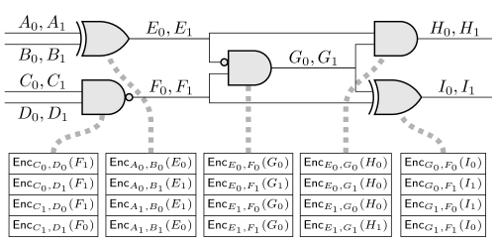
\includegraphics[width=1.0\textwidth]{Chapter2/Figs/Raster/garbledCircuit}
  \caption{Garbled Circuit example}
  \label{fig:garbledCircuit}
\end{figure}

Recent work provides optimizations to improve the computation and communication
overhead associated with encrypt/decrypt operations and ciphertext tables'
sizes. In \cite{kolesnikov2008improved30}, the authors proposed a modification
to allow XOR gates to be evaluated \textit{for free}: the labels of XOR gates
are not chosen independently but by \(\omega_{i,0} = \omega_{i,1} \xor r\), for
some random value of \(r\). Pinkas et al. \cite{pinkas2009secure38} introduced a
way to reduce the communication size of binary gates by 25\%: each gate can be
specified by three ciphertexts instead of all four. Finally,
\cite{kolesnikov2009improved29} improve some commonly used circuits such as
addition, comparision, etc., by reducing the number of non-XOR gates.

\subsection{Using GC with Homomorphic Encryption in the protocol}
\label{sec:finalcontr}
We use a standard substractor circuit for the operation \(HD = HD' - r\): Given
a 2 n-bit bitstring, the circuit is built from 1 half-substractor and \(n-1\)
full-substractors as in Figure \ref{fig:substractor}, where a half-substractor
is built from 1 XOR gate and 1 AND gate, a full-substractor is built from 2
half-substractors and 1 OR gate (Figure \ref{fig:fullSubstractor})

\begin{figure}[htbp!] 
  \centering    
  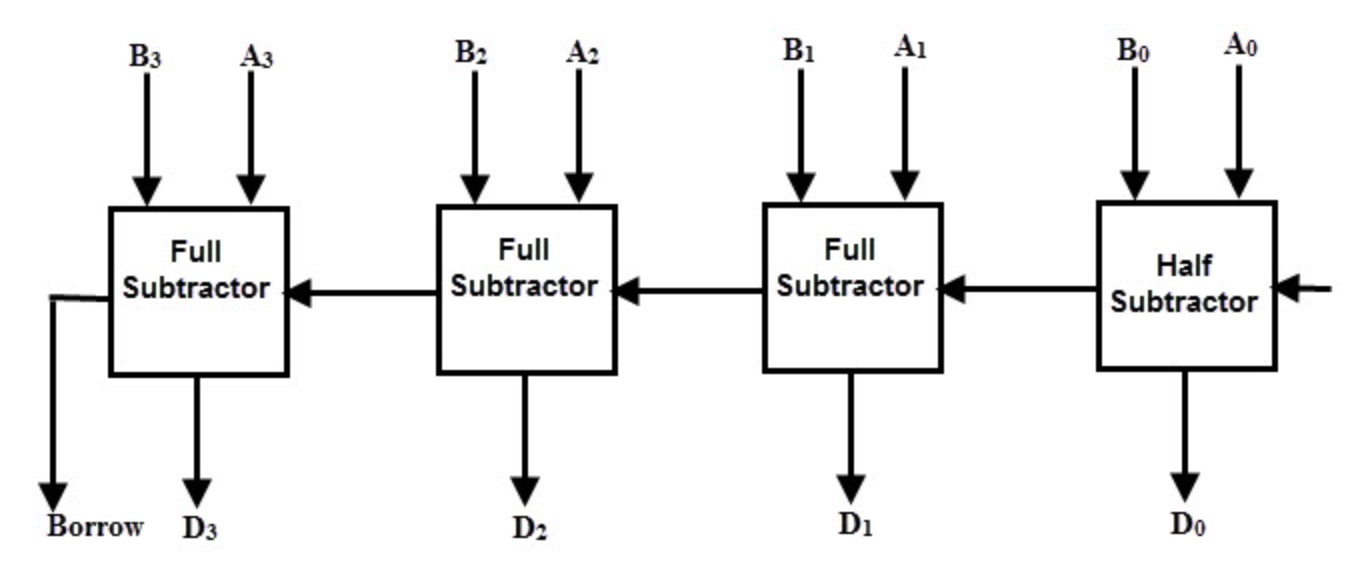
\includegraphics[width=1.0\textwidth]{Chapter7/Figs/Raster/subCircuit}
  \caption{Substractor Circuit}
  \label{fig:substractor}
\end{figure}



\begin{figure}[htbp!] 
  \centering    
  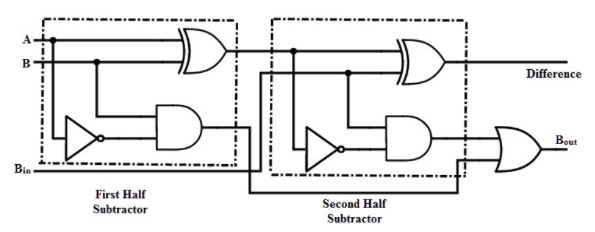
\includegraphics[width=1.0\textwidth]{Chapter7/Figs/Raster/fullSubstractor}
  \caption{Half-substractor and Full-substractor}
  \label{fig:fullSubstractor}
\end{figure}

In our context, let \(l\) be the bit length of the HD' and r (\(l\) is typically
10-12 bits for 1024-2048 bits biometrics data), which makes the number of
substractor logic gates equal to \(5l\). The comparision circuit no longer needs
to output 3 results (as a standard circuits would: Either A > B, A < B or A =
B). Our aim is just to check whether \(HD' - r < \tau\), so we simply need to
have l NAND gates plus \(l-1\) XOR gates at hand for the comparsion
circuit. Figure \ref{fig:comparisionCircuit1} shows an example of such a
configuration
\begin{figure}[htbp!] 
  \centering    
  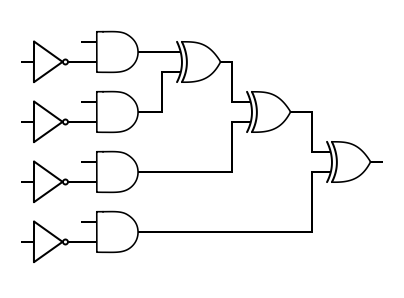
\includegraphics[scale=0.75]{Chapter7/Figs/Raster/comparisionCircuit}
  \caption{Comparator Circuit}
  \label{fig:comparisionCircuit1}
\end{figure}

\paragraph{Garbled Circuit preparation}
We denote \(GC\) to be the garbled circuit prepared by the server. The inputs to
the circuit include the server's \(GC_{r}\) and the client's \(GC_{h}\), which
are the cryptographic key \textit{labels} corresponding to the server's input
\(r\) and to the client's input \(HD'\) to the function \textit{CompareHD}. The main
function of the circuit is, first, to substract \(HD' - r = HD\) then compare
\(HD \stackrel{?}{<} \tau\), where \(\tau\) is the constant value of the
threshold required to decide upon the authentication result, which can be built into the
circuit itself. We note that either the server or the client can play the role of
setting up the garbled circuit; in our work, we let the server take this role
(Figure \ref{fig:fourthProtocol} - Step 5, 6, 7, 8): as we have
been working on a \textit{semi-honest} server modeal and a \textit{malicious }
client, this will save us one proof to assess that the circuit is generated
correctly.

As pointed out previously, the server garbles the circuit \(GC\) and sends the
result to the client together with its \textit{labels} of \(r\), which are
\(K_{r_{i}}^{j}\). Next, the client uses our OT technique (discussed in the
following section) to select the correct \textit{labels} of \(HD'\): the first
part of the OT will ensure that the client will get back the encryptions
\(\enc{K_{h_{i}}^{j}}\). The second part of the OT makes sure that the protocol
is secure against \textit{malicious} clients: it needs to prove that it
decrypted and decomposed \(\enc{\mathbf{HD'}}\) correctly (Figure
\ref{fig:fourthProtocol} - Step 12,13). In other words, the client wants to
prove that the encryptions \(\enc{h_{i}}\) it sent are actually the encryptions
of the bits of \(HD'_{i}\). Recall that the server still has
\(\enc{\mathbf{HD'}}\), so the proof can be a homomorphical check of
\(\enc{\mathbf{HD'}} - \sum{2^{i}\enc{h_{i}}} = \enc{0}\). However, in order to
allow this proof to support homomorphic operations, we need to use the same
encryption scheme for the OT protocol, in other words, we need an OT protocol
based on BGV. In the next section, we discuss a this novel solution to the problem of
interfacing Garbled Circuit with Homomorphic Encryption.

We note that inside the garbled circuit, AES is normally used to encrypt the
\textit{labels}, this encryption is a part of the garbled circuit and not
related to the OT protocol we just described, and can still be used independently
to ensure the performance of circuit evaluations. Next, we discuss an approach
to design an OT protocol compatible with the BGV cryptosystem

\subsection{Oblivious Transfer}
\label{sec:obliviousTransferPre}

\textit{"You take the blue pill, the story ends. You wake up in your bed and
  believe whatever you want to believe. You take the red pill, you stay in
  wonderland, and I show you how deep the rabbit hole goes."} - Morpheus to Neo,
The Matrix.


\begin{figure}[htbp!] 
\centering    
\includegraphics[width=1.0\textwidth]{Chapter2/Figs/Raster/RedPillBluePill}
\caption[Minion]{Red Pill - Blue Pill}
\label{fig:RedPillBluePill}
\end{figure}

What if, in such situation, there were a protocol to give privacy to
\(Neo\): \(Morpheus\) should not be able to discover what option \(Neo\) has chosen. Moreover, the
protocol can also provide privacy to \(Morpheus\): \(Neo\) being thus unable to get information about the unchosen pill. In cryptography, Oblivious Transfer (OT) is a
protocol able to support such a scenario. 
In its most basic form, it is a
two-parties protocol between a \textit{Sender} and a \textit{Receiver}, denoted
by \(\begin{psmallmatrix} 2 \\ 1 \end{psmallmatrix} \)-OT. The \(Sender\) uses
two private inputs \(x_{0}, x_{1}\) and the \(Receiver\) uses one input bit
\(s\). At the completion of the protocol, the \(Receiver\) gets the bit
\(x_{s}\), without letting the \(Sender\) acquire any information about the value of
\(s\): \(\begin{psmallmatrix} 2 \\ 1 \end{psmallmatrix}
\)-OT\((x_{0},x_{1};s) = x_{s}\).

The general idea is that, when the receiver requests an item, the sender sends
all the available items to him, unaware of which one has been requested. However, the response is encrypted in such a way that the receiver
can only decrypt the one he requested. A concrete implementation example of the
\(\begin{psmallmatrix} 2 \\ 1 \end{psmallmatrix} \)-OT protocol based on
discrete log DH is illustrated in figure \ref{fig:DH21OT} (This protocol is
secure against \textit{honest but curious} attacks). The receiver picks
\(h_{0},h_{1}\) such that \(h_{0}h_{1} = h\), he cannot access both
\(\log_{g}h_{0}\) and \(\log_{g}h_{1}\). Given \(h_{0}, h_{1}\), the sender
returns ElGamal encryptions of bits \(x_{0}, x_{1}\) using \(h_{0},h_{1}\) as
public keys. The receiver then decrypts one of the encryptions to recover either
\(x_{0} \text{ or } x_{1}\)

\begin{figure}[htbp!] 
  \centering
  \procedure{DH-based Protocol}{
    \textbf{Sender} \> \> \textbf{Receiver}\\
    (x_0, x_1 \in \{0,1\}) \> \> (s \in \{0,1\})\\
    \> \> u \randomsample \mathbb{Z}n \\
    \> \> h_s \gets g^u \\
    \> \sendmessageleft*{h_0, h_1} \> h_{1 - s} \gets h/g^u \\
    u_0, u_1 \randomsample \mathbb{Z}_n \> \> \\
    (A_0, B_0) \gets (g^{u_0}, h_0^{u_0}g^{x_0}) \> \> \\
    (A_1, B_1) \gets (g^{u_1}, h_1^{u_1}g^{x_1}) \> \sendmessageright*{(A_0, B_0), (A_1, B_1)} \> x_s \gets \log_g{(B_s/A_s^u)} \\
  }
  \caption{OT protocol based on DH}
  \label{fig:DH21OT}
\end{figure}

Efficient implementations of Oblivious Transfer can be found in
\cite{naor2001efficient35}. The techniques found in \cite{ishai2003extending24}
can reduce a large number of OT protocol executions to \(\lambda\), where
\(\lambda\) is the security parameter.

\subsection{The BGV-based Oblivious Transfer protocol}
\label{sec:finalContr2}
In this thesis, we propose a new OT
technique to be used with lattice-based cryptosystems. The technique can be used
together with the garbled circuit protocol discussed earlier. The problem can be
stated as follows: Given a BGV ciphertext of a bit selection \(h_{i}\):
\(\enc{h_{i}}\), the server computes and returns a BGV encryption of the
corresponding key selected by the bit. We observe that the following homomorphic
operations will satisfy such a requirement:
\[
\enc{K_{i}^{j}} = \enc{h_{i}^{j}} \cdot \enc{K_{i}^{1}} + (1 - \enc{h_{i}^{j}}) \cdot \enc{K_{i}^{0}}
\]
where \(K_{i}^{0}, K_{i}^{1}\) are the \textit{labels} corresponding to the wire
inputs 0 or 1. The function includes one level of homomorphic multiplication, two
additions and one multiplication with a constant. This approach is simple enough
and it is secure against a \textit{malicious client} model in our context because
the client needs to prove that he actually encrypted \(\enc{h_{i}}\)
correctly already. Other applications of this OT should take into account that a
malicious client can encrypt \(\enc{h_{i}}\) incorrectly to obtain information about
\(K_{i}^{0}\) and/or \(K_{i}^{1}\).

The other issue that we have to be careful about is \textit{Circuit Privacy}:
for a multi-factor attacker able to access the secret key but not the
biometric template, it is possible to obtain information about the randomness of the
operation. The randomness of the above operation is of the form
\(K_{i}^{0} + (K_{i}^{1} - K_{i}^{0})r_{0}\), which is correlated to both
keys. Again, we can mask the randomness of this leakage similarly to what we did
in the second variant of the protocol. By a similar analysis, we can still show
that computing the HD cannot be achieved with a significant level of probability (the privacy
security requirement related to what the client sees is indistinguishable
from the probability he has to compute the HD, which is not much more than random
guessing).

% \begin{figure}[h!]
%   \centering
%   \begin{equation*}
%     \begin{array}{c c c}
%       \text{\textbf{Sender}} & & \text{\textbf{Receiver}} \\
%       \\
%       (x_{0}, x_{1} \in \{0,1\}) & & (s \in \{0,1\}) \\
%                              & & u \randomsample \mathbb{Z}_{n}\\
%                              & & h_{s} \gets g^{u}\\
%                              & & h_{1-s} \gets h/g^{u}\\
%                              & \xleftarrow{h_{0}, h_{1}} & \\
%       u_{0}, u_{1} \randomsample \mathbb{Z}_{n} & & \\
%       (A_{0}, B_{0}) \gets (g^{u_{0}}, h_{0}^{u_{0}}g^{x_{0}}) & & \\
%       (A_{1}, B_{1}) \gets (g^{u_{1}}, h_{1}^{u_{1}}g^{x_{1}}) & & \\
%                              & \xrightarrow{(A_{0}, B_{0}),(A_{1}, B_{1})} & \\
%       & & x_{s} \gets \log_{g}(B_{s}/A_{s}^{u})
%     \end{array}
%   \end{equation*}
%   \caption{OT protocol based on DH}
%   \label{fig:DH21OT}
% \end{figure}



\section{The details}
\label{sec:4thProcDetails}

\subsection{The protocol description}
\label{sec:4thprocSteps}
With a notation similar to the one used for previous protocols, we describe the last variant of the authentication system as follows (Figure \ref{fig:fourthProtocol})
\begin{enumerate}
\item In the enrollment stage, the client $\user$ extracts his template $\enc{\mathbf{T}}$ and sends it to the server $\server$
\item In the authentication stage, $\user$ extracts his query template $\enc{\mathbf{Q}}$ and sends it to the server
\item $\user$ uses a Schnorr-based ZKP (Section \ref{sec:zkpschnorr}) to prove that the noise associated with $\enc{\mathbf{Q}}$ is small
\item $\user$ uses the Challenge-Response technique (Section \ref{sec:challengeResponse}) to prove that $\enc{\mathbf{Q}}$ is encrypting a binary message
\item If the proofs pass, $\server$ starts preparing the garbled circuit $GC$, it first samples $r \randomsample \mathbb{Z}_{t}$ and decomposes it into a binary representation, assuming that $r$ is $k$ bits long.
\item $\server$ establishes $k$ pair of keys $(K_{r_{i}}^{0}, K_{r_{i}}^{1})$ for the inputs of $GC_{r}$
\item $\server$ establishes $k$ pair of keys $(K_{h_{i}}^{0}, K_{h_{i}}^{1})$ for the inputs of $GC_{h}$
\item $\server$ establishes the pair of keys for authentication result outputs $(K_{out}^{0}, K_{out}^{1})$
\item $\server$ encrypts the $k$ keys of $GC_{h}$ to obtain $\enc{K_{h_{i}}^{0}}, \enc{K_{h_{i}}^{1}}$
\item $\server$ computes $\enc{HD} \gets HDBGV(\enc{\mathbf{T}}, \enc{\mathbf{Q}})$
\item $\server$ masks the Hamming Distance $\enc{\mathbf{HD'}} = \enc{\mathbf{HD + r}}$ and sends the result together with the garbled ciruit $GC$ and the keys $K_{r_{i}}^{j}$ to $\user$, where $j$ associates the key of $GC_{r}$ corresponding to the $r$ chosen by $\server$.
\item $\user$ decrypts $\enc{\mathbf{HD}'}$
\item $\user$ decomposes the plaintext $HD'$ into its binary representation $HD' = \sum_{0}^{k-1}2^{i}h_{i}$
\item $\user$ re-encrypts the bits of the decomposition
\item $\user$ uses the ciphertext $\enc{h_{i}}$ in the Oblivious Transfer Protocol (Section \ref{sec:obliviousTransferPre}) to retrieve the ciphertexts $\enc{K_{h_{i}}^{j}}$
\item $\user$ decrypts the result to obtain another set of keys for the garbled circuit
\item $\user$ evaluates the circuit with the keys $(K_{h_{i}}^{j}, K_{r_{i}}^{j})$ and sends the result to the server
\item $\server$ compares this outcome with the output keys prepared in step 8 and outputs the final authentication result.
\end{enumerate}

\begin{figure}[htbp!] 
  \centering \procedure{The Fourth Protocol}{
    \textbf{Client} \> \> \textbf{Server}\\
    \text{1. Registered template \textbf{T}} \> \sendmessageright*{\enc{\mathbf{T}}} \> \text{Store } \enc{\mathbf{T}}\\
    \text{2. Query template \textbf{Q}} \> \sendmessageright*{\enc{\mathbf{Q}}} \> \text{Initiate Query Proof}\\
    \> \sendmessageleft*{\text{3. Prove small noise in \textbf{Q}}} \> \\
    \> \sendmessageleft*{\text{4. Prove \textbf{Q} is binary}} \> \\
    \> \> \text{Sample \(r \randomsample \mathbb{Z}_{t}\)}\\
    \> \> \text{5. Setup garbled circuit GC, for } i = 1,\dots,k \\
    \> \> \text{6. Setup } (K^{0}_{r_{i}}, K^{1}_{r_{i}}) \text{ for } GC_r \\
    \> \> \text{7. Setup } (K^{0}_{h_{i}}, K^{1}_{h_{i}}) \text{ for } GC_{h}\\
    \> \> \text{8. Setup } (K^{0}_{out}, K^{1}_{out}) \\
    \> \> \text{9. Compute } \enc{K^0_{h_i}},\enc{K^1_{h_i}}\\
    \> \> \text{10. } \enc{\mathbf{HD}} = HDBGV(\enc{\mathbf{T}},\enc{\mathbf{Q}}) \\
    \> \> \text{Compute } \enc{\mathbf{HD'}} = \enc{\mathbf{HD + r}}\\
    \> \sendmessageleft*{\enc{\mathbf{HD'}}} \> \\
    \> \sendmessageleft*{GC} \> \\
    \> \sendmessageleft*{K_{r_i}^j \text{of } GC_r} \> \\
    \text{12. Decrypt } \mathbf{HD'} = dec(\enc{\mathbf{HD}}) \> \> \\
    \text{13. Decompose } \mathbf{HD'} = \sum_{i=0}^k{2^ih_i} \> \> \\
    \text{14. Encrypt } \enc{h_i} \> \> \\
    \text{15. Initiate OT protocol} \> \> \\
    \> \sendmessageright*{16. \enc{h_i}} \> \\
    \> \sendmessageright*{\text{17. Prove correct decryption}} \> \\
    \> \sendmessageleft*{\text{18. Retrieve } \enc{K_{h_i}^j}} \> \\
    \text{19. Decrypt } K_{h_i}^j \> \> \\
    20. K_{out} = GC( K_{h_i}^j , K_{r_i}^j) \> \> \\
    \> \sendmessageright*{K_{out}} \> \text{21. Compare } K_{out} \text{ with } K_{out}^0, K_{out}^1 \\
    \> \> \text{ Output res = \textbf{Accept|Reject}}
  }
  \caption{The fourth Protocol}
  \label{fig:fourthProtocol}
\end{figure}

\subsection{Implementation Result}
\label{sec:7result}
We observe significant improvements in communication size thanks to the
Challenge-Response technique (only 2 messages required). The Schnorr-based ZKP
also contributes to this factor by reducing the number of rounds in proofs to 1,
instead of 17 for similar settings
$(n = 2048, t = 2048, \alpha q = 8, q \approx 2^{72}, FAR \approx
10^{-3})$. The total number of gates used in the garbled circuit for $n=2048$ equals 25, which only cost $\approx 3.2$ KB for the HD comparison purpose. All of
these improvements come with a one time setup cost for preparing the switch keys
for the HD computation operation: we need to rotate 10 times and swap 1 time to
compute $HD$, each operation needs 1 key switch to transform the result back to
the original ciphertext format (2 ring elements) before the next homomorphic
operation. The total key switch size needed is $2*n*\log q*11$, which is
approximately 389 MB in our setting. Considering the privacy features provided,
we believe such one time set up cost is acceptable. We conclude the chapter with
the comparison of the 4 protocols described in the thesis

\begin{table}[h!]
\centering
\caption{Protocols' features comparison}
\label{my-label}
\begin{tabular}{lllll}
\hline
                                          & \textbf{Multi-factor}    & \textbf{HD Non-exposure} & \textbf{Low Init cost} & \textbf{Low Communication} \\ \hline
\multicolumn{1}{|l|}{\textbf{Protocol 1}} & \multicolumn{1}{l|}{No}  & \multicolumn{1}{l|}{No}        & \multicolumn{1}{l|}{Yes}   & \multicolumn{1}{l|}{Yes}   \\ \hline
\multicolumn{1}{|l|}{\textbf{Protocol 2}} & \multicolumn{1}{l|}{Yes} & \multicolumn{1}{l|}{No}        & \multicolumn{1}{l|}{Yes}   & \multicolumn{1}{l|}{Yes}   \\ \hline
\multicolumn{1}{|l|}{\textbf{Protocol 3}} & \multicolumn{1}{l|}{Yes} & \multicolumn{1}{l|}{Yes}       & \multicolumn{1}{l|}{Yes}   & \multicolumn{1}{l|}{No}    \\ \hline
\multicolumn{1}{|l|}{\textbf{Protocol 4}} & \multicolumn{1}{l|}{Yes} & \multicolumn{1}{l|}{Yes}       & \multicolumn{1}{l|}{No}    & \multicolumn{1}{l|}{Yes}   \\ \hline
\end{tabular}
\end{table}
    
% \begin{figure}[h!]
%   \centering
%     \begin{equation*}
%         \begin{array}{c c c}
%         \text{\textbf{Client}} & & \text{\textbf{Server}} \\
%           \\
%           \text{1. Registered template \textbf{T}} & \xrightarrow{\enc{\mathbf{T}}} & \text{Store } \enc{\mathbf{T}}\\
          
%           \text{2. Query template \textbf{Q}} & \xrightarrow{\enc{\mathbf{Q}}} & \text{Initiate Query Proof}\\

%                                & \xleftrightarrow{\text{3. Prove small noise in \textbf{Q}}} & \\

%                                & \xleftrightarrow{\text{4. Prove \textbf{Q} is binary}} & \\

%                                & & \text{Sample \(r \randomsample \mathbb{Z}_{t}\)}\\
%                                & & \text{5. Setup garbled circuit GC, for } i = 1,\dots,k \\

%                                & & \text{6. Setup } (K^{0}_{r_{i}}, K^{1}_{r_{i}}) \text{ for } GC_r \\
          
%                                & & \text{7. Setup } (K^{0}_{h_{i}}, K^{1}_{h_{i}}) \text{ for } GC_{h}\\
          
%                                & & \text{8. Setup } (K^{0}_{out}, K^{1}_{out}) \\

%                                & & \text{9. Compute } \enc{K^0_{h_i}},\enc{K^1_{h_i}}\\
%           \\

%                                & & \text{10. } \enc{\mathbf{HD}} = HDBGV(\enc{\mathbf{T}},\enc{\mathbf{Q}}) \\
          
%                                    & & \text{Compute } \enc{\mathbf{HD'}} = \enc{\mathbf{HD + r}}\\

%                                & \xleftarrow{\enc{\mathbf{HD'}}} & \\

%                                & \xleftarrow{GC} & \\

%                                & \xleftarrow{K_{r_i}^j \text{of } GC_r} & \\

%           \text{12. Decrypt } \mathbf{HD'} = dec(\enc{\mathbf{HD}}) & & \\

%           \text{13. Decompose } \mathbf{HD'} = \sum_{i=0}^k{2^ih_i} & & \\

%           \text{14. Encrypt } \enc{h_i} & & \\
          
%           \text{15. Initiate OT protocol} & & \\

%                                & \xrightarrow{16. \enc{h_i}} & \\
          
%                                & \xrightarrow{\text{17. Prove correct decryption}} & \\

%                                & \xleftarrow{\text{18. Retrieve } \enc{K_{h_i}^j}} & \\

%           \text{19. Decrypt } K_{h_i}^j & & \\
%           20. K_{out} = GC( K_{h_i}^j , K_{r_i}^j) & & \\

%                                & \xrightarrow{K_{out}} & \text{21. Compare } K_{out} \text{ with } K_{out}^0, K_{out}^1 \\
%           & & \text{ Output res = \textbf{Accept|Reject}}
%         \end{array}
%     \end{equation*}

%   \caption{The fourth protocol}
%   \label{fig:fourthProtocol}
% \end{figure}


% \section{Related Work}
% \label{sec:chap7RelatedWorks}



% Consider the following situation:  How can he achieve that?
% Suppose that the plaintext \(P\) is encoded as coefficients of a polynomial, or
% specifically, \(P\) can be an element of the ring \(R_{2}\), where
% \(R_{2} = \frac{\mathbb{Z}_{2}[x]}{x^{n} + 1}\), this ring has been used by many
% RLWE based cryptosystems lately. One solution can be to apply the Zero Knowlege
% Proof technique. This is however a costly choice. There are mainly two
% approaches for ZKP, the Schnorr's based protocol,
% e.g. \cite{benhamouda2014better} or a Stern's based protocol such as
% \cite{stern1993new} or \cite{ling2013improved}. The first approach has
% limitations on the norm of the secret it can prove and cannot be used to prove
% the knowledge of binary messages with norm 2. The second approach can prove
% binary messages but it has a very high communication cost due to a roundness
% error equaling \(2/3\).
% \subsection{ZKP and $\sum$-Protocol}
% \label{sub:zkp_and_sum_protocol}
% A Zero-Knowledge Proof of Knowledge (ZKPoK) is a two party protocol between a
% Prover $P$ and a Verifier $V$. The protocol allows $P$ to convince $V$ that it
% knows some secret without revealing anything about the secret. We refer readers
% to \cite{bellare1992defining} for formal definition of the original ZKPoK. 

% Notation: 




% \subsection{Schnorr-based ZKP technique}
% \label{sec:zero-knowledge-proof}


% \begin{figure}[htbp!] 
%   \centering \procedure{AND-Composition of Benhamouda ZKP}{
%     \textbf{Prover} \> \> \textbf{Verifier}\\
%     \mathbf{r_s,r_{e_0},r'_{s},r'_{e_{0}}} \randomsample D_{\beta_0} \> \> \\
%     \mathbf{r_e,r'_{e}} \randomsample D_{\beta} \> \> \\
%     \mathbf{r_m,r'_{m}} \randomsample D_{t} \> \> \\
%     \mathbf{t_c} = \mathbf{-c_1r_s} + t\mathbf{r_e + r_m} \> \> \\
%     \mathbf{t_k} = \mathbf{-p_1r_s} - t\mathbf{r_{e_0}} \> \> \\
%     \mathbf{t'_c} = \mathbf{-c_1r'_s} + t\mathbf{r'_e + r'_m} \> \> \\
%     \mathbf{t'_k} = \mathbf{-p_1r'_s} - t\mathbf{r'_{e_0}} \> \> \\
%     (c_{aux}, d_{aux}) = aCommit(\mathbf{t_c,t_k}) \> \> \\
%     (c'_{aux}, d'_{aux}) = aCommit(\mathbf{t'_c,t'_k}) \>
%     \sendmessageright*{c_{aux},c'_{aux}} \> \\
%     \> \> c \randomsample \mathcal{C} = \left\{ 0,\dots, 2n -1  \right\}\\
%     \>  \sendmessageleft*{c} \> \\
%     \mathbf{s_s = r_s + x^cs},\mathbf{s'_s = r'_s + x^cs} \> \> \\
%     \mathbf{s_e = r_e + x^ce},\mathbf{s'_e = r'_e + x^ce} \> \> \\
%     \mathbf{s_m = r_m + x^cm},\mathbf{s'_m = r'_m + x^cm} \> \> \\
%     \mathbf{s_{e_0} = r_{e_0} + x^ce_0},\mathbf{s'_{e_0} = r'_{e_0} + x^ce_0} \> \> \\
%     \> \sendmessageright{top=$d_{aux}$, bottom=$d'_{aux}$} \> \\
%     \> \> \mathbf{x^cc_0} + \mathbf{t_c} \stackrel{?}{=} -\mathbf{c_1s_s} + t\mathbf{s_e} + \mathbf{s_m}\\
%     \> \> \mathbf{x^cc_0} + \mathbf{t'_c} \stackrel{?}{=} -\mathbf{c_1s'_s} + t\mathbf{s'_e} + \mathbf{s'_m}\\
%     \> \> \mathbf{x^cp_0} + \mathbf{t_k} \stackrel{?}{=} -\mathbf{p_1s_s} - t\mathbf{s_{e_0}}\\
%     \> \> \mathbf{x^cp_0} + \mathbf{t'_k} \stackrel{?}{=} -\mathbf{p_1s'_s} - t\mathbf{s'_{e_0}}\\
%     \> \> aCOpen(\mathbf{t_c, t_k}, c_{aux}, d_{aux}) \stackrel{?}{=} accept \\
%     \> \> aCOpen(\mathbf{t'_c, t'_k}, c'_{aux}, d'_{aux}) \stackrel{?}{=} accept \\
%     \> \> \norm{s_s}, \norm{s_{e_0}},\norm{s'_s}, \norm{s'_{e_0}} \leq 2\beta_0 \\
%     \> \> \norm{s_e},\norm{s'_e}  \leq 2\beta \\
%     \> \> \norm{s_m},\norm{s'_m} \leq 2t
%   }
%   \caption{AND-Composition for ZKP-BV}
%   \label{fig:belhamoudaProtocolAND}
% \end{figure}

  % \begin{figure}[h!]
  %   \centering
  %   \begin{equation*}
  %     \begin{array}{c c c}
  %       \text{\textbf{Prover}} & & \text{\textbf{Verifier}} \\
  %       \\
  %       \mathbf{r_s,r_{e_0},r'_{s},r'_{e_{0}}} \randomsample D_{\beta_0} & & \\
  %       \mathbf{r_e,r'_{e}} \randomsample D_{\beta} & & \\
  %       \mathbf{r_m,r'_{m}} \randomsample D_{t} & & \\
  %       \mathbf{t_c} = \mathbf{-c_1r_s} + t\mathbf{r_e + r_m} & & \\
  %       \mathbf{t_k} = \mathbf{-p_1r_s} - t\mathbf{r_{e_0}} & & \\
  %       \mathbf{t'_c} = \mathbf{-c_1r'_s} + t\mathbf{r'_e + r'_m} & & \\
  %       \mathbf{t'_k} = \mathbf{-p_1r'_s} - t\mathbf{r'_{e_0}} & & \\
  %       (c_{aux}, d_{aux}) = aCommit(\mathbf{t_c,t_k}) & & \\
  %       (c'_{aux}, d'_{aux}) = aCommit(\mathbf{t'_c,t'_k}) &
  %                                                        \xrightarrow{\hspace{1em}c_{aux},c'_{aux}\hspace{1em}} & \\
  %                              & & c \randomsample \mathcal{C} = \left\{ 0,\dots, 2n -1  \right\}\\
  %                              &  \xleftarrow{\hspace{1em}c\hspace{1em}} & \\
  %       \mathbf{s_s = r_s + x^cs},\mathbf{s'_s = r'_s + x^cs} & & \\
  %       \mathbf{s_e = r_e + x^ce},\mathbf{s'_e = r'_e + x^ce} & & \\
  %       \mathbf{s_m = r_m + x^cm},\mathbf{s'_m = r'_m + x^cm} & & \\
  %       \mathbf{s_{e_0} = r_{e_0} + x^ce_0},\mathbf{s'_{e_0} = r'_{e_0} + x^ce_0} & & \\
  %                              & \xrightarrow[\hspace{1em}d'_{aux}, \mathbf{t'_c, t'_k, s'_s, s'_e, s'_m,
  %                                s'_{e_0}}\hspace{1em}]{\hspace{1em}d_{aux}, \mathbf{t_c, t_k, s_s, s_e, s_m,
  %                                s_{e_0}}\hspace{1em}} & \\
  %                              & & \mathbf{x^cc_0} + \mathbf{t_c} \stackrel{?}{=} -\mathbf{c_1s_s} + t\mathbf{s_e} + \mathbf{s_m}\\
  %                              & & \mathbf{x^cc_0} + \mathbf{t'_c} \stackrel{?}{=} -\mathbf{c_1s'_s} + t\mathbf{s'_e} + \mathbf{s'_m}\\
  %                              & & \mathbf{x^cp_0} + \mathbf{t_k} \stackrel{?}{=} -\mathbf{p_1s_s} - t\mathbf{s_{e_0}}\\
  %                              & & \mathbf{x^cp_0} + \mathbf{t'_k} \stackrel{?}{=} -\mathbf{p_1s'_s} - t\mathbf{s'_{e_0}}\\
  %                              & & aCOpen(\mathbf{t_c, t_k}, c_{aux}, d_{aux}) \stackrel{?}{=} accept \\
  %                              & & aCOpen(\mathbf{t'_c, t'_k}, c'_{aux}, d'_{aux}) \stackrel{?}{=} accept \\
  %                              & & \norm{s_s}, \norm{s_{e_0}},\norm{s'_s}, \norm{s'_{e_0}} \leq 2\beta_0 \\
  %                              & & \norm{s_e},\norm{s'_e}  \leq 2\beta \\
  %                              & & \norm{s_m},\norm{s'_m} \leq 2t
  %     \end{array}
  %   \end{equation*}
  %   \caption{AND-Composition for ZKP-BV }
  %   \label{fig:belhamoudaProtocolAND}
  % \end{figure}


% \subsection{Combination of ZKP}
% \label{sec:combination-zkp}
% A $\sum-$protocol can be composed together to construct more complex relations.
% There are several forms of decomposition such as AND, OR, NEQ, etc.  We describe
% some forms of composition of the \(\sum-protocol\) that are used in our own protocol:
% AND-composition, OR-composition. We first describe the generic \(\sum-\)protocol
% and its combinations. The BV-ZKP (Figure \ref{fig:belhamoudaProtocol}) protocol
% is an instance of such a protocol and the technique can be applied inherently.
% \begin{description}
% \item[$\sum-$protocol] The protocol is a generic 3-moves transaction between 2 parties
%   \(Prover\) and \(Verifier\), it is used to prove (supporting zero-knowledge) a
%   relation \(R(x,w)\), where \(x\) is the public parameter known by both
%   parties and \(w\) is a witness known by the \(Prover\) only. The protocol's
%   view is a set of 3 messages (Figure \ref{fig:sigmaProtocol}): the commitment
%   \(c\) is a function of a random factor \(\rho\), the challenge \(ch\) is
%   normally random, and the response \(r\) is a function computed from
%   \(x, w, \rho, ch\). There are 2 extra algorithms for the \(\sum-\)protocol: a
%   \(verify(r,ch,c)\) algorithm used by the \(Verifier\) in the last step to
%   check the correctness of the proof result, and a simulator \(sim\), taking
%   \(x\) and a random parameter \(\rho'\) as inputs, and and outputting a view
%   \(\bar{c},\bar{ch},\bar{r}\) that is indistinguishable from the genuine view
%   of the protocol.

%   \begin{figure}[htbp!] 
%     \centering \procedure{Sigma Protocol}{
%       \textbf{Prover} \> \> \textbf{Verifier}\\
%       \rho \randomsample random \> \> \\
%       c \gets comm(\rho) \> \> \\
%       \> \sendmessageright*{c} \> \\
%       \> \> ch \randomsample random \\
%       \> \sendmessageleft*{ch} \> \\
%       r \gets resp(\rho,w,x,ch) \> \> \\
%       \> \sendmessageright*{r} \> \\
%       \> \> verify(r, ch, c)\\
%     }
%     \caption{Sigma Protocol}
%     \label{fig:sigmaProtocol}
%   \end{figure}
%   % \begin{figure}[h!]
%   %   \centering
%   %   \begin{equation*}
%   %     \begin{array}{c c c}
%   %       \text{\textbf{Prover}} & & \text{\textbf{Verifier}} \\
%   %       \\
%   %       \rho \randomsample random & & \\
%   %       c = comm(\rho) & & \\
%   %                              & \xrightarrow{c} & \\
%   %                              & & ch \randomsample random \\
%   %                              & \xleftarrow{ch} & \\
%   %       r = resp(\rho,w,x,ch) & & \\
%   %                              & \xrightarrow{r} & \\
%   %                              & & verify(r, ch, c)\\
%   %     \end{array}
%   %   \end{equation*}
%   %   \caption{Sigma Protocol}
%   %   \label{fig:sigmaProtocol}
%   % \end{figure}
% \end{description}


% \begin{description}
% \item[AND-COMPOSITION] Given two relations $R_1 = \left\{ (v_1,w_1) \right\}$
%   and $R_2 = \left\{ (v_2, w_2) \right\}$ with the same challenge space, a
%   $\sum$-Protocol of
%   $R_1 \wedge R_2 = \left\{ (v_1, v_2, w_1, w_2): (v_1;w_1) \in R_1, (v_2,w_2)
%     \in R_2\right\}$ can be obtained by running a $\sum$-Protocol for $R_1$ and
%   a $\sum$-Protocol for $R_2$ in parallel, using a \emph{common} challenge.
%   Figure \ref{fig:belhamoudaProtocolAND} is a concrete example combining 2 ZKP for BV.
  

% \item[OR-Compostion] In this composition, given the $\sum-protocol$ for many  
%   relations $R_{1}$,$R_{2}$,\dots,\(R_{n}\) the goal is to construct a protocol for the
%   relation
%   $R_{OR}(\vec{x}, w_{i}) $, where \(\exists i \leq n: R(x_{i},w_{i}) = 1\). The main reason behind this composition is that the verifier
%   can let the prover use the simulator of the \(\sum-protocol\) for the
%   relations \(R_{j}\), for which the prover does not know the witness.
%   The verifier provides a single challenge \(c\)
%   such that the prover can split that into challenges \(c_{1}, c_{2}, \dots, c_{n}\)
%   provided that \(c_{i}\) satisfies a linear constraint in terms of \(c\),
%   for example \(c = c_{1} \xor c_{2} \xor \dots \xor c_{n}\). The final OR-combination proof is
%   obtained by composing one run of the \(\sum-protocol\) with other runs of the
%   simulators for the \(\sum-protocol\). (Figure \ref{fig:OR-Combination})

%   \begin{figure}[htbp!] 
%     \centering \procedure{OR Composition of ZKP}{
%       \textbf{Prover} \> \> \textbf{Verifier}\\
%       \rho_{i} \randomsample random \> \> \\
%       c_{i} = comm(\rho_{i}) \> \> \\
%       \text{For } j = 1,\dots,n \wedge j \neq i: \> \> \\
%       \text{    } \rho_{j} \randomsample random; \> \> \\
%       \text{    } (c_{j}, ch_{j}, r_{j}) \gets ZKPSim(\rho_{j}, x_{j}) \> \> \\
%       \> \sendmessageright*{ch_j,c_{1}, c_{2}, \dots, c_{n}} \> \\
%       \> \> ch \randomsample \mathbb{Z}_{n} \\
%       \> \sendmessageleft*{ch} \> \\
%       ch_{i} = ch - \sum_{j \neq i}{ch_{j}} \> \> \\
%       r_{i} = resp(\rho_{i}, w_{i}, x_{i}, ch_{i}) \> \> \\
%       \> \sendmessageright*{r_{1}, r_{2}, \dots, r_{n}} \> \\
%       \> \> \forall i \in [n], ver(r_{i}, ch_{i}, c_{i}) = 1 \\
%       \> \> ch = \sum_{i \in [n]}ch_{i}\\
%     }
%     \caption{OR Composition of ZKP}
%     \label{fig:OR-Composition}
%   \end{figure}
  % \begin{figure}[h!]
  %   \centering
  %   \begin{equation*}
  %     \begin{array}{c c c}
  %       \text{\textbf{Prover}} & & \text{\textbf{Verifier}} \\
  %       \\
  %       \rho_{i} \randomsample random & & \\
  %       c_{i} = comm(\rho_{i}) & & \\
  %       \text{For } j = 1,\dots,n \wedge j \neq i: & & \\
  %       \text{    } \rho_{j} \randomsample random; & & \\
  %       \text{    } (c_{j}, ch_{j}, r_{j}) \gets ZKPSim(\rho_{j}, x_{j}) & & \\
  %                              & \xrightarrow[ch_{j}]{c_{1}, c_{2}, \dots, c_{n}} & \\
  %                              & & ch \randomsample \mathbb{Z}_{n} \\
  %                              & \xleftarrow{ch} & \\
  %       ch_{i} = ch - \sum_{j \neq i}{ch_{j}} & & \\
  %       r_{i} = resp(\rho_{i}, w_{i}, x_{i}, ch_{i}) & & \\
  %                              & \xrightarrow{r_{1}, r_{2}, \dots, r_{n}} & \\
  %                              & & \forall i \in [n], ver(r_{i}, ch_{i}, c_{i}) = 1 \\
  %                              & & ch = \sum_{i \in [n]}ch_{i}\\
  %     \end{array}
  %   \end{equation*}
  %   \caption{}
  %   \label{fig:OR-Combination}
  % \end{figure}
% \end{description}





%%% Local Variables:
%%% mode: latex
%%% TeX-master: "../thesis"
%%% End:

% \subsection*{Summary of previous work}
% \begin{description}
% \item Lyubashevsky's proof systems (\cite{lyubashevsky2008lattice},
%   \cite{lyubashevsky2009fiat}): This system is similar to the classical Schnorr's
%   ZKP system, the main advantage is its communication size efficiency. However,
%   this approach is not zero-knowledge (it is only proved to be witness
%  -indistinguishable). Moreover, there is a completeness error in each round, and
%   lastly, the extraction gap is $O(\sqrt{n})$.

%   A quick discussion on extraction gaps: we refer to an extraction gap as a security
%   parameter of ZKP systems for ISIS problem. Generally, we say that a proof accepts
%   an extraction gap $\gamma$ ($\gamma > 1$) if the knowledge extractor of the
%   protocol can extract a vector $\vec{v}$ such that
%   $\norminf{v} = \gamma \norminf{w}$, where $\norminf{w}$ is a valid witness
%   from the \emph{Prover}. Ideally, when $\gamma = 1$, one can use the extractor
%   to solve the underlying ISIS instance. In other words, ZKP with $\gamma = 1$
%   is strongly secure, as breaking it is at least as hard as solving the
%   underlying problem. When $\gamma > 1$, the soundness of the proof has to rely
%   on a stronger hardness assumption of certain potentially easier problems is hard
%   to solve.
% \item Micciancio-Vadhan proof system \cite{micciancio2003statistical}: This
%   protocol provides ZKP for the GapCVP problem, but it can be adapted to prove the ISIS
%   relation: Let $\mathbf{B}$ be a basis of the perp lattice
%   $\Lambda_q^\bot(\mathbf{A}) = \{\mathbf{x} \in \mathbb{Z}^m: \mathbf{A.x = 0}\
%   \mod \ q\}$.  and $\mathbf{t} \in \mathbb{Z}^m: \mathbf{A.t = y}\ \mod \ q$
%   ($\mathbf{B}$ and $\mathbf{t}$ can be computed efficiently), then run the ZKP
%   protocol for $GapCVP_\gamma^\infty$ with public parameters
%   $(\mathbf{B,t},\beta$). The $Prover$'s witness is $\mathbf{e = t - x}$. Recall
%   that The knowledge extractor of the protocol can output a vector
%   $\mathbf{e'} \in \Lambda_q^\bot( \mathbf{A}$ such that
%   $\norminf{\mathbf{ t - e'}} \leq g.\beta$ for some $g \geq O(\sqrt[]
%   {m}$). This implies a perfect ZKPoPK with extraction gap $O(\sqrt[]{m})$.
% \item Stern's protocol [\todo{citeStern}] and extension: The original Stern's
%   proof worked on the SD relation \todo{SD relation}. This ZKP does not have any
%   completeness error and there is no extraction gap, i.e., $\gamma =
%   1$. Extensions of this work include KTX [137,85], associated with the
%   following relation \todo{ktxRelation}.

%   The work of \cite{ling2013improved} provides a proof for the ISIS relation
%   \todo{ISIS relation}.  Stern's based techniques inherently do not have
%   extraction gaps nor completeness errors, their communication efficiency is:
%   \todo{missing figure}. Our protocol will also be based on this technique, the
%   enhancement being that it can prove different bounds of different elements in the
%   $Prover$'s witness vector. Such improvement is important in ZKPoPK for
%   lattice-based cryptosystems, especially in contexts where public key settings
%   and homomorphic operations are used. The bounds of messages and errors can be
%   largely different: for example, the original message can be binary while the
%   noises' bounds increase according to the ladder of homomorphic operations.

% \end{description}






%%% Local Variables:
%%% mode: latex
%%% TeX-master: "../thesis"
%%% End:




% ********************************** Back Matter *******************************
% Backmatter should be commented out, if you are using appendices after References
%\backmatter

% ********************************** Bibliography ******************************
\begin{spacing}{0.9}

% To use the conventional natbib style referencing
% Bibliography style previews: http://nodonn.tipido.net/bibstyle.php
% Reference styles: http://sites.stat.psu.edu/~surajit/present/bib.htm

\bibliographystyle{apalike}
%\bibliographystyle{unsrt} % Use for unsorted references  
%\bibliographystyle{plainnat} % use this to have URLs listed in References
\cleardoublepage
\bibliography{global} % Path to your References.bib file


% If you would like to use BibLaTeX for your references, pass `custombib' as
% an option in the document class. The location of 'reference.bib' should be
% specified in the preamble.tex file in the custombib section.
% Comment out the lines related to natbib above and uncomment the following line.

%\printbibliography[heading=bibintoc, title={References}]


\end{spacing}

% ********************************** Appendices ********************************

\begin{appendices} % Using appendices environment for more functunality

% ******************************* Thesis Appendix A ****************************
\chapter{How to install \LaTeX} 

\section*{Windows OS}

\subsection*{TeXLive package - full version}
\begin{enumerate}
\item	Download the TeXLive ISO (2.2GB) from\\
\href{https://www.tug.org/texlive/}{https://www.tug.org/texlive/}
\item	Download WinCDEmu (if you don't have a virtual drive) from \\
\href{http://wincdemu.sysprogs.org/download/}
{http://wincdemu.sysprogs.org/download/}
\item	To install Windows CD Emulator follow the instructions at\\
\href{http://wincdemu.sysprogs.org/tutorials/install/}
{http://wincdemu.sysprogs.org/tutorials/install/}
\item	Right click the iso and mount it using the WinCDEmu as shown in \\
\href{http://wincdemu.sysprogs.org/tutorials/mount/}{
http://wincdemu.sysprogs.org/tutorials/mount/}
\item	Open your virtual drive and run setup.pl
\end{enumerate}

or

\subsection*{Basic MikTeX - \TeX~ distribution}
\begin{enumerate}
\item	Download Basic-MiK\TeX (32bit or 64bit) from\\
\href{http://miktex.org/download}{http://miktex.org/download}
\item	Run the installer 
\item	To add a new package go to Start >> All Programs >> MikTex >> Maintenance (Admin) and choose Package Manager
\item	Select or search for packages to install
\end{enumerate}

\subsection*{TexStudio - \TeX~ editor}
\begin{enumerate}
\item	Download TexStudio from\\
\href{http://texstudio.sourceforge.net/\#downloads}
{http://texstudio.sourceforge.net/\#downloads} 
\item	Run the installer
\end{enumerate}

\section*{Mac OS X}
\subsection*{MacTeX - \TeX~ distribution}
\begin{enumerate}
\item	Download the file from\\
\href{https://www.tug.org/mactex/}{https://www.tug.org/mactex/}
\item	Extract and double click to run the installer. It does the entire configuration, sit back and relax.
\end{enumerate}

\subsection*{TexStudio - \TeX~ editor}
\begin{enumerate}
\item	Download TexStudio from\\
\href{http://texstudio.sourceforge.net/\#downloads}
{http://texstudio.sourceforge.net/\#downloads} 
\item	Extract and Start
\end{enumerate}


\section*{Unix/Linux}
\subsection*{TeXLive - \TeX~ distribution}
\subsubsection*{Getting the distribution:}
\begin{enumerate}
\item	TexLive can be downloaded from\\
\href{http://www.tug.org/texlive/acquire-netinstall.html}
{http://www.tug.org/texlive/acquire-netinstall.html}.
\item	TexLive is provided by most operating system you can use (rpm,apt-get or yum) to get TexLive distributions
\end{enumerate}

\subsubsection*{Installation}
\begin{enumerate}
\item	Mount the ISO file in the mnt directory
\begin{verbatim}
mount -t iso9660 -o ro,loop,noauto /your/texlive####.iso /mnt
\end{verbatim}

\item	Install wget on your OS (use rpm, apt-get or yum install)
\item	Run the installer script install-tl.
\begin{verbatim}
	cd /your/download/directory
	./install-tl
\end{verbatim}
\item	Enter command `i' for installation

\item	Post-Installation configuration:\\
\href{http://www.tug.org/texlive/doc/texlive-en/texlive-en.html\#x1-320003.4.1}
{http://www.tug.org/texlive/doc/texlive-en/texlive-en.html\#x1-320003.4.1} 
\item	Set the path for the directory of TexLive binaries in your .bashrc file
\end{enumerate}

\subsubsection*{For 32bit OS}
For Bourne-compatible shells such as bash, and using Intel x86 GNU/Linux and a default directory setup as an example, the file to edit might be \begin{verbatim}
edit $~/.bashrc file and add following lines
PATH=/usr/local/texlive/2011/bin/i386-linux:$PATH; 
export PATH 
MANPATH=/usr/local/texlive/2011/texmf/doc/man:$MANPATH;
export MANPATH 
INFOPATH=/usr/local/texlive/2011/texmf/doc/info:$INFOPATH;
export INFOPATH
\end{verbatim}
\subsubsection*{For 64bit OS}
\begin{verbatim}
edit $~/.bashrc file and add following lines
PATH=/usr/local/texlive/2011/bin/x86_64-linux:$PATH;
export PATH 
MANPATH=/usr/local/texlive/2011/texmf/doc/man:$MANPATH;
export MANPATH 
INFOPATH=/usr/local/texlive/2011/texmf/doc/info:$INFOPATH;
export INFOPATH

\end{verbatim}



%\subsection{Installing directly using Linux packages} 
\subsubsection*{Fedora/RedHat/CentOS:}
\begin{verbatim} 
sudo yum install texlive 
sudo yum install psutils 
\end{verbatim}


\subsubsection*{SUSE:}
\begin{verbatim}
sudo zypper install texlive
\end{verbatim}


\subsubsection*{Debian/Ubuntu:}
\begin{verbatim} 
sudo apt-get install texlive texlive-latex-extra 
sudo apt-get install psutils
\end{verbatim}

% ******************************* Thesis Appendix B ********************************

\chapter{Installing the CUED class file}

\LaTeX.cls files can be accessed system-wide when they are placed in the
<texmf>/tex/latex directory, where <texmf> is the root directory of the user’s \TeX installation. On systems that have a local texmf tree (<texmflocal>), which
may be named ``texmf-local'' or ``localtexmf'', it may be advisable to install packages in <texmflocal>, rather than <texmf> as the contents of the former, unlike that of the latter, are preserved after the \LaTeX system is reinstalled and/or upgraded.

It is recommended that the user create a subdirectory <texmf>/tex/latex/CUED for all CUED related \LaTeX class and package files. On some \LaTeX systems, the directory look-up tables will need to be refreshed after making additions or deletions to the system files. For \TeX Live systems this is accomplished via executing ``texhash'' as root. MIK\TeX users can run ``initexmf -u'' to accomplish the same thing.

Users not willing or able to install the files system-wide can install them in their personal directories, but will then have to provide the path (full or relative) in addition to the filename when referring to them in \LaTeX.

\end{appendices}

% *************************************** Index ********************************
\printthesisindex % If index is present

\end{document}

%%% Local Variables:
%%% mode: latex
%%% TeX-master: t
%%% End:
